\documentclass[tese,capa,english]{texufpel}

%\usepackage{mathpazo}
%\usepackage[mathpazo]{flexisym}

%\usepackage[utf8]{inputenc} % acentuacao
\usepackage{graphicx} % para inserir figuras
\usepackage[T1]{fontenc}
\usepackage{amsmath} % to use overset
\usepackage{wasysym} % to use circles
\usepackage{semantic} % for inference rules
\usepackage{amsthm} % for proof environment
\usepackage{mathtools} % to use arrows with text
\usepackage{stackengine} % to break lines on inference rules

\hypersetup{
    hidelinks, % Remove coloração e caixas
    unicode=true,   %Permite acentuação no bookmark
    linktoc=all %Habilita link no nome e página do sumário
}

\unidade{Centro de Desenvolvimento Tecnol\'{o}gico}
\programa{Programa de P\'{o}s-Gradua\c{c}\~{a}o em Computa\c{c}\~{a}o}
\curso{Ci\^{e}ncia da Computa\c{c}\~{a}o}

\unidadeeng{Centro de Desenvolvimento Tecnol\'{o}gico}
\programaeng{Postgraduate Program in Computing}
\cursoeng{Computer Science}

\title{Strategies for Testing and Formalizing Properties of \\Modern Programming Languages}

\author{Feitosa}{Samuel da Silva}
\advisor[Prof.~Dr.]{Du Bois}{Andre Rauber}
\coadvisor[Prof.~Dr.]{Ribeiro}{Rodrigo Geraldo}
%\collaborator[Prof.~Dr.]{Aguiar}{Marilton Sanchotene de}

%Palavras-chave em PT_BR
\keyword{Palavrachave-um}
\keyword{Palavrachave-dois}
\keyword{Palavrachave-tres}
\keyword{Palavrachave-quatro}

%Palavras-chave em EN_US
\keywordeng{Keyword-one}
\keywordeng{Keyword-two}
\keywordeng{Keyword-three}
\keywordeng{Keyword-four}

%%%%%%%%%%%%%%%%%%%%%% THEOREMS AND PROOFS %%%%%%%%%%%%%%%%%%%%%%%%%%%%%%%%%%%%%

\newtheorem{theorem}{Theorem}
\newtheorem{lemma}{Lemma}

%%%%%%%%%%%%%%%%%%%%%%%%%%%%%%%%%%%%%%%%%%%%%%%%%%%%%%%%%%%%%%%%%%%%%%%%%%%%%%%%

%%%%%%%%%%%%%%%%%%%%%%%%%%%%%%%%%%%%%%%%%%%%%%%%%%%%%%%%%%%%%%%%%%%%%%%%%%%%%%%%
%%                        Begin of lts2TeX stuff                              %%
%%%%%%%%%%%%%%%%%%%%%%%%%%%%%%%%%%%%%%%%%%%%%%%%%%%%%%%%%%%%%%%%%%%%%%%%%%%%%%%%

%% ODER: format ==         = "\mathrel{==}"
%% ODER: format /=         = "\neq "
%
%
\makeatletter
\@ifundefined{lhs2tex.lhs2tex.sty.read}%
  {\@namedef{lhs2tex.lhs2tex.sty.read}{}%
   \newcommand\SkipToFmtEnd{}%
   \newcommand\EndFmtInput{}%
   \long\def\SkipToFmtEnd#1\EndFmtInput{}%
  }\SkipToFmtEnd

\newcommand\ReadOnlyOnce[1]{\@ifundefined{#1}{\@namedef{#1}{}}\SkipToFmtEnd}
\usepackage{amstext}
\usepackage{amssymb}
\usepackage{stmaryrd}
\DeclareFontFamily{OT1}{cmtex}{}
\DeclareFontShape{OT1}{cmtex}{m}{n}
  {<5><6><7><8>cmtex8
   <9>cmtex9
   <10><10.95><12><14.4><17.28><20.74><24.88>cmtex10}{}
\DeclareFontShape{OT1}{cmtex}{m}{it}
  {<-> ssub * cmtt/m/it}{}
\newcommand{\texfamily}{\fontfamily{cmtex}\selectfont}
\DeclareFontShape{OT1}{cmtt}{bx}{n}
  {<5><6><7><8>cmtt8
   <9>cmbtt9
   <10><10.95><12><14.4><17.28><20.74><24.88>cmbtt10}{}
\DeclareFontShape{OT1}{cmtex}{bx}{n}
  {<-> ssub * cmtt/bx/n}{}
\newcommand{\tex}[1]{\text{\texfamily#1}}	% NEU

\newcommand{\Sp}{\hskip.33334em\relax}


\newcommand{\Conid}[1]{\mathit{#1}}
\newcommand{\Varid}[1]{\mathit{#1}}
\newcommand{\anonymous}{\kern0.06em \vbox{\hrule\@width.5em}}
\newcommand{\plus}{\mathbin{+\!\!\!+}}
\newcommand{\bind}{\mathbin{>\!\!\!>\mkern-6.7mu=}}
\newcommand{\rbind}{\mathbin{=\mkern-6.7mu<\!\!\!<}}% suggested by Neil Mitchell
\newcommand{\sequ}{\mathbin{>\!\!\!>}}
\renewcommand{\leq}{\leqslant}
\renewcommand{\geq}{\geqslant}
\usepackage{polytable}

%mathindent has to be defined
\@ifundefined{mathindent}%
  {\newdimen\mathindent\mathindent\leftmargini}%
  {}%

\def\resethooks{%
  \global\let\SaveRestoreHook\empty
  \global\let\ColumnHook\empty}
\newcommand*{\savecolumns}[1][default]%
  {\g@addto@macro\SaveRestoreHook{\savecolumns[#1]}}
\newcommand*{\restorecolumns}[1][default]%
  {\g@addto@macro\SaveRestoreHook{\restorecolumns[#1]}}
\newcommand*{\aligncolumn}[2]%
  {\g@addto@macro\ColumnHook{\column{#1}{#2}}}

\resethooks

\newcommand{\onelinecommentchars}{\quad-{}- }
\newcommand{\commentbeginchars}{\enskip\{-}
\newcommand{\commentendchars}{-\}\enskip}

\newcommand{\visiblecomments}{%
  \let\onelinecomment=\onelinecommentchars
  \let\commentbegin=\commentbeginchars
  \let\commentend=\commentendchars}

\newcommand{\invisiblecomments}{%
  \let\onelinecomment=\empty
  \let\commentbegin=\empty
  \let\commentend=\empty}

\visiblecomments

\newlength{\blanklineskip}
\setlength{\blanklineskip}{0.66084ex}

\newcommand{\hsindent}[1]{\quad}% default is fixed indentation
\let\hspre\empty
\let\hspost\empty
\newcommand{\NB}{\textbf{NB}}
\newcommand{\Todo}[1]{$\langle$\textbf{To do:}~#1$\rangle$}

\EndFmtInput
\makeatother
%
%
%
%
%
%
% This package provides two environments suitable to take the place
% of hscode, called "plainhscode" and "arrayhscode". 
%
% The plain environment surrounds each code block by vertical space,
% and it uses \abovedisplayskip and \belowdisplayskip to get spacing
% similar to formulas. Note that if these dimensions are changed,
% the spacing around displayed math formulas changes as well.
% All code is indented using \leftskip.
%
% Changed 19.08.2004 to reflect changes in colorcode. Should work with
% CodeGroup.sty.
%
\ReadOnlyOnce{polycode.fmt}%
\makeatletter

\newcommand{\hsnewpar}[1]%
  {{\parskip=0pt\parindent=0pt\par\vskip #1\noindent}}

% can be used, for instance, to redefine the code size, by setting the
% command to \small or something alike
\newcommand{\hscodestyle}{}

% The command \sethscode can be used to switch the code formatting
% behaviour by mapping the hscode environment in the subst directive
% to a new LaTeX environment.

\newcommand{\sethscode}[1]%
  {\expandafter\let\expandafter\hscode\csname #1\endcsname
   \expandafter\let\expandafter\endhscode\csname end#1\endcsname}

% "compatibility" mode restores the non-polycode.fmt layout.

\newenvironment{compathscode}%
  {\par\noindent
   \advance\leftskip\mathindent
   \hscodestyle
   \let\\=\@normalcr
   \let\hspre\(\let\hspost\)%
   \pboxed}%
  {\endpboxed\)%
   \par\noindent
   \ignorespacesafterend}

\newcommand{\compaths}{\sethscode{compathscode}}

% "plain" mode is the proposed default.
% It should now work with \centering.
% This required some changes. The old version
% is still available for reference as oldplainhscode.

\newenvironment{plainhscode}%
  {\hsnewpar\abovedisplayskip
   \advance\leftskip\mathindent
   \hscodestyle
   \let\hspre\(\let\hspost\)%
   \pboxed}%
  {\endpboxed%
   \hsnewpar\belowdisplayskip
   \ignorespacesafterend}

\newenvironment{oldplainhscode}%
  {\hsnewpar\abovedisplayskip
   \advance\leftskip\mathindent
   \hscodestyle
   \let\\=\@normalcr
   \(\pboxed}%
  {\endpboxed\)%
   \hsnewpar\belowdisplayskip
   \ignorespacesafterend}

% Here, we make plainhscode the default environment.

\newcommand{\plainhs}{\sethscode{plainhscode}}
\newcommand{\oldplainhs}{\sethscode{oldplainhscode}}
\plainhs

% The arrayhscode is like plain, but makes use of polytable's
% parray environment which disallows page breaks in code blocks.

\newenvironment{arrayhscode}%
  {\hsnewpar\abovedisplayskip
   \advance\leftskip\mathindent
   \hscodestyle
   \let\\=\@normalcr
   \(\parray}%
  {\endparray\)%
   \hsnewpar\belowdisplayskip
   \ignorespacesafterend}

\newcommand{\arrayhs}{\sethscode{arrayhscode}}

% The mathhscode environment also makes use of polytable's parray 
% environment. It is supposed to be used only inside math mode 
% (I used it to typeset the type rules in my thesis).

\newenvironment{mathhscode}%
  {\parray}{\endparray}

\newcommand{\mathhs}{\sethscode{mathhscode}}

% texths is similar to mathhs, but works in text mode.

\newenvironment{texthscode}%
  {\(\parray}{\endparray\)}

\newcommand{\texths}{\sethscode{texthscode}}

% The framed environment places code in a framed box.

\def\codeframewidth{\arrayrulewidth}
\RequirePackage{calc}

\newenvironment{framedhscode}%
  {\parskip=\abovedisplayskip\par\noindent
   \hscodestyle
   \arrayrulewidth=\codeframewidth
   \tabular{@{}|p{\linewidth-2\arraycolsep-2\arrayrulewidth-2pt}|@{}}%
   \hline\framedhslinecorrect\\{-1.5ex}%
   \let\endoflinesave=\\
   \let\\=\@normalcr
   \(\pboxed}%
  {\endpboxed\)%
   \framedhslinecorrect\endoflinesave{.5ex}\hline
   \endtabular
   \parskip=\belowdisplayskip\par\noindent
   \ignorespacesafterend}

\newcommand{\framedhslinecorrect}[2]%
  {#1[#2]}

\newcommand{\framedhs}{\sethscode{framedhscode}}

% The inlinehscode environment is an experimental environment
% that can be used to typeset displayed code inline.

\newenvironment{inlinehscode}%
  {\(\def\column##1##2{}%
   \let\>\undefined\let\<\undefined\let\\\undefined
   \newcommand\>[1][]{}\newcommand\<[1][]{}\newcommand\\[1][]{}%
   \def\fromto##1##2##3{##3}%
   \def\nextline{}}{\) }%

\newcommand{\inlinehs}{\sethscode{inlinehscode}}

% The joincode environment is a separate environment that
% can be used to surround and thereby connect multiple code
% blocks.

\newenvironment{joincode}%
  {\let\orighscode=\hscode
   \let\origendhscode=\endhscode
   \def\endhscode{\def\hscode{\endgroup\def\@currenvir{hscode}\\}\begingroup}
   %\let\SaveRestoreHook=\empty
   %\let\ColumnHook=\empty
   %\let\resethooks=\empty
   \orighscode\def\hscode{\endgroup\def\@currenvir{hscode}}}%
  {\origendhscode
   \global\let\hscode=\orighscode
   \global\let\endhscode=\origendhscode}%

\makeatother
\EndFmtInput
%

\usepackage{color}
\newcommand{\redFG}[1]{\textcolor[rgb]{0.6,0,0}{#1}}
\newcommand{\greenFG}[1]{\textcolor[rgb]{0,0.5,0}{#1}}
\newcommand{\blueFG}[1]{\textcolor[rgb]{0,0,0.8}{#1}}
\newcommand{\orangeFG}[1]{\textcolor[rgb]{0.8,0.4,0}{#1}}
\newcommand{\purpleFG}[1]{\textcolor[rgb]{0.4,0,0.4}{#1}}
\newcommand{\yellowFG}[1]{\textcolor[rgb]{0.8,0.33,0.0}{#1}}
\newcommand{\brownFG}[1]{\textcolor[rgb]{0.5,0.2,0.2}{#1}}
\newcommand{\blackFG}[1]{\textcolor[rgb]{0.06,0.06,0.06}{#1}}
\newcommand{\whiteFG}[1]{\textcolor[rgb]{1,1,1}{#1}}
\newcommand{\pinkFG}[1]{\textcolor[rgb]{1.0,0.0,0.5}{#1}}
\newcommand{\yellowBG}[1]{\colorbox[rgb]{1,1,0.2}{#1}}
\newcommand{\brownBG}[1]{\colorbox[rgb]{1.0,0.7,0.4}{#1}}

\newcommand{\ColourStuff}{
  \newcommand{\red}{\redFG}
  \newcommand{\green}{\greenFG}
  \newcommand{\blue}{\blueFG}
  \newcommand{\orange}{\orangeFG}
  \newcommand{\purple}{\purpleFG}
  \newcommand{\yellow}{\yellowFG}
  \newcommand{\brown}{\brownFG}
  \newcommand{\black}{\blackFG}
  \newcommand{\white}{\whiteFG}
  \newcommand{\pink}{\pinkFG}
}

\newcommand{\MonochromeStuff}{
  \newcommand{\red}{\blackFG}
  \newcommand{\green}{\blackFG}
  \newcommand{\blue}{\blackFG}
  \newcommand{\orange}{\blackFG}
  \newcommand{\purple}{\blackFG}
  \newcommand{\yellow}{\blackFG}
  \newcommand{\brown}{\blackFG}
  \newcommand{\black}{\blackFG}
  \newcommand{\white}{\blackFG}
  \newcommand{\pink}{\blackFG}
}

\ColourStuff

\newcommand{\K}[1]{\yellow{\mathsf{#1}}}
\newcommand{\D}[1]{\blue{\mathsf{#1}}}
\newcommand{\Con}[1]{\green{\mathsf{#1}}}
\newcommand{\F}[1]{\blue{\mathsf{#1}}}
\newcommand{\V}[1]{\black{\mathsf{#1}}}
\newcommand{\N}[1]{\red{\mathsf{#1}}}
\newcommand{\RF}[1]{\pink{\mathsf{#1}}}
\newcommand{\Comm}[1]{\red{\textnormal{#1}}}
% Haskell 
\newcommand{\HK}[1]{\purple{\mathsf{#1}}}
\newcommand{\HT}[1]{\green{\mathsf{#1}}}
\newcommand{\HC}[1]{\green{\mathsf{#1}}}
\newcommand{\HFun}[1]{\blue{\mathsf{#1}}}
\newcommand{\HS}[1]{\yellow{\mathsf{#1}}}
\newcommand{\HN}[1]{\red{\mathsf{#1}}}
% Java
\newcommand{\JK}[1]{\purple{\mathsf{#1}}}
\newcommand{\JC}[1]{\green{\mathsf{#1}}}
\newcommand{\JM}[1]{\blue{\mathsf{#1}}}

\DeclareMathAlphabet{\mathkw}{OT1}{cmss}{bx}{n}

%%%%%%%%%%%%%%%%%%%%%%%%%%%%%%%%%%%%%%%%%%%%%%%%%%%%%%%%%%%%%%%%%%%%%%%%%%%%%%%%
%%                          End of lhs2Tex stuff                              %%
%%%%%%%%%%%%%%%%%%%%%%%%%%%%%%%%%%%%%%%%%%%%%%%%%%%%%%%%%%%%%%%%%%%%%%%%%%%%%%%%

\begin{document}

%\renewcommand{\advisorname}{Orientadora}           %descomente caso tenhas orientadora
%\renewcommand{\coadvisorname}{Coorientadora}      %descomente caso tenhas coorientadora

\maketitle 

\sloppy

\fichacatalografica

%Composição da Banca Examinadora
\begin{aprovacao}{20 de dezembro de 2019} %data da banca por extenso
\noindent Prof. Dr. Andre Rauber Du Bois (orientador)\\
Doutorado em Ci\^{e}ncia da Computa\c{c}\~{a}o pela Heriot-Watt University, Esc\'{o}cia.\\[1cm]

\noindent Prof. Dr. Alvaro Freitas Moreira.\\
Doutorado em Ci\^{e}ncia da Computa\c{c}\~{a}o pela University of Edinburgh, Esc\'{o}cia.\\[1cm]

\noindent Prof. Dr. Juliana Kaizer Vizzotto\\
Doutorado em Computa\c{c}\~{a}o pela Universidade Federal do Rio Grande do Sul.\\[1cm]

\noindent Prof. Dr. Luciana Foss\\
Doutorado em Computa\c{c}\~{a}o pela Universidade Federal do Rio Grande do Sul.
\end{aprovacao}

%Opcional
\begin{dedicatoria}
  To my wife Cheila, for her kindness and devotion, and her endless support.
\end{dedicatoria}

%Opcional
\begin{agradecimentos}
  First and foremost, I would like to thank my parents for their love and support throughout my life. Thank you both for encourage me to pursue my dreams.

\vspace{5pt}
  
  I am profoundly grateful to my thesis advisers, Prof. Andr\'{e} Rauber Du Bois, and Prof. Rodrigo Geraldo Ribeiro, for their guidance and support throughout this study and especially for their confidence in me. I also would like to thank Prof. Wouter Swierstra and Prof. Alejandro Serrano Mena for their kindness support during my studies abroad.

\vspace{5pt}
  
  %I would also like to acknowledge Prof. Alvaro Freitas Moreira, Prof. Juliana Kaizer Vizzotto, and Prof. Luciana Foss, as the board examiners of this doctorate defense. I am gratefully indebted to them for their very valuable comments on this thesis.

% \vspace{5pt}
  
  Last but not least, I thank for having my wife Cheila during all this time, sharing the good and bad moments, always understanding and encouraging me to keep working hard toward my goals. Your partnership is what makes me grow.

\vspace{5pt}
  
  This material was based upon work supported by CAPES/Brazil. % - Finance code 001.
  
\vspace{15pt}
  
  This thesis is only the beginning of my journey.

\end{agradecimentos}

%Opcional
\begin{epigrafe}
  If debugging is the process of removing software bugs, \\ programming must be the process of putting them in.\\
  {\sc --- Edsger Dijkstra}
\end{epigrafe}

%Resumo em Inglês (no maximo 500 palavras)
\begin{abstract}
  Today's world is full of devices and machines controlled by software, which depend upon programming languages and compilers to be produced and executed. The importance of correct software development goes beyond personal computers and smartphone apps. An error in a critical system, such as on a nuclear power plant or on an airplane controller, can cause catastrophic damage in our society. Nowadays, essentially two software validation techniques are used to avoid such problems: software testing and software verification.

  In this thesis we combine both validation techniques in the programming languages research area, applying property-based testing first to improve specifications and debugging programs, before an attempt of formal verification. By using such testing approach we can quickly eliminate false conjectures, by using the generated counterexamples, which help to correct them. Then, having confidence that the specification is correct, one can give a step forward and formalize the specification and prove its properties in an interactive theorem prover, which uses a mathematical framework to guarantee that these properties hold for a given specification.

  We apply different strategies to test and formalize two major programming languages, the functional Lambda Calculus, and the modern object-oriented calculus Featherweight Java. The first branch of this thesis defines a type-directed procedure to generate random programs for each calculus in order to apply property-based testing to check soundness properties on them, using the Haskell library QuickCheck. And in the second branch, we apply the two most used approaches, extrinsic and intrinsic, to formalize and prove type safety for both studied programming languages using the dependently-typed programming language Agda, comparing the subtleties of each technique. Furthermore, we shown that our formalizations can be extended to new language constructions, by specifying and proving the same properties for the Java 8 constructions. We believe that this combination of property-based testing with formal verification can improve the quality of software in general and increase the productivity during formal proof development.
  
\end{abstract}

\begin{englishabstract}{Estrat\'{e}gias para Teste e Formaliza\c{c}\~{a}o de Propriedades de Linguagens de Programa\c{c}\~{a}o}
O mundo atual est\'{a} repleto de dispositivos e m\'{a}quinas controladas por software, os quais dependem de linguagens de programa\c{c}\~{a}o e compiladores para serem produzidos e executados. A import\^{a}ncia do desenvolvimento de software correto vai al\'{e}m de computadores pessoais e aplicativos de smartphones. Um erro em um sistema cr\'{i}tico, como em uma usina nuclear ou em um controlador de avia\c{c}\~{a}o, pode causar danos catastr\'{o}ficos em nossa sociedade. Hoje em dia, essencialmente duas t\'{e}cnicas de valida\c{c}\~{a}o de software s\~{a}o utilizadas para evitar tais problemas: teste e verifica\c{c}\~{a}o de software. 

Nesta tese, s\~{a}o combinadas ambas as t\'{e}cnicas de valida\c{c}\~{a}o na \'{a}rea pesquisa de linguagens de programa\c{c}\~{a}o, aplicando testes baseados em propriedades inicialmente para melhorar especifica\c{c}\~{o}es e depurar programas, antes de uma tentativa de verifica\c{c}\~{a}o formal. Por usar esta abordagem de testes, \'{e} poss\'{i}vel eliminar falsas conjecturas rapidamente e usar os contra-exemplos gerados para corrig\'{i}-las. Ent\~{a}o, tendo confian\c{c}a de que a especifica\c{c}\~{a}o est\'{a} correta, \'{e} poss\'{i}vel ir al\'{e}m, formalizando a especifica\c{c}\~{a}o e provando propriedades em um provador de teoremas interativo, o qual usa um aparato matem\'{a}tico para garantir que estas propriedades s\~{a}o v\'{a}lidas para uma dada especifica\c{c}\~{a}o.

Aplicou-se diferentes estrat\'{e}gias para testar e formalizar duas linguages de programa\c{c}\~{a}o, o C\'{a}lculo Lambda, e o c\'{a}lculo orientado a objetos Featherweight Java. A primeira parte desta tese define um procedimento direcionado por tipos para gerar programas aleat\'{o}rios para cada linguagem de modo a aplicar testes baseados em propriedades para verificar propriedades de seguran\c{c}a, usando Haskell e a biblioteca QuickCheck. E, na segunda parte, foram aplicadas duas abordagens, extr\'{i}nseca e intr\'{i}nseca, para formalizar e provar seguran\c{c}a de tipos para ambas as linguagens de programa\c{c}\~{a}o estudadas, usando a linguagem de tipos dependentes Agda, comparando as sutilezas de cada t\'{e}cnica. Al\'{e}m disso, foi demonstrado que as formaliza\c{c}\~{o}es apresentadas podem ser estendidas para novas constru\c{c}\~{o}es de linguagens, a partir da especifica\c{c}\~{a}o e provas das mesmas propriedades para as constru\c{c}\~{o}es da linguagem Java 8. Acredita-se que esta combina\c{c}\~{a}o de testes baseados em propriedades com verifica\c{c}\~{a}o formal pode melhorar a qualidade de software em geral e aumentar a produtividade durante o desenvolvimento de provas formais.
  
\end{englishabstract}

%Lista de Figuras
\listoffigures

%Lista de Tabelas
\listoftables

%lista de abreviaturas e siglas
\begin{listofabbrv}{STLC}%coloque aqui a maior sigla para ajustar a distância
        \item[AST] Abstract Syntax Tree
        \item[BNF] Backus-Naur Form
        \item[FJ] Featherweight Java
        \item[JDK] Java Development Kit
        \item[JVM] Java Virtual Machine
        \item[LC] Lambda Calculus
        \item[LOC] Lines of Code
        \item[STLC] Simply Typed Lambda Calculus
\end{listofabbrv}

%Sumario
\tableofcontents

\chapter{Introduction}

Programming languages are applied in every computational problem, from simple applications, such as smartphone apps, to complex critical systems, like those for flight control. Therefore, it is important to have mechanisms to verify that a programming language indeed implements certain behavior and enjoys some desired properties. Typically, the development of compilers (or interpreters) of major programming languages in the industry relies on dynamic analysis (testing) for detecting and eliminating bugs. On the other hand, most of the research about programming languages is done using static analysis (proving properties) for producing correct implementations. Both techniques have pros and cons. Testing can be done easily, using several well-studied approaches, producing counter-examples of the specification which can be used to fix the implementation faster. However, only by testing, it is impossible to prove the absence of errors. Theorem proving can provide such guarantees, however, in spite of continuous progress in the area, the process of mechanizing properties is still very time consuming and requires good skills from the user. Our methodology applies one branch of the testing area, called property-based testing, to improve specifications and to debug interpreters, before proving properties on a proof assistant.

Property-based testing is an automated approach to testing in which a program is validated against a specification, using randomly generated input data, in order to find counterexamples for the property being checked. Applying property-based testing for compilers or programming language semantics is not an easy task, because it is difficult to design a random generator for valid programs. Generating good test cases can be tricky, since these programs should have a structure that is accepted by the compiler, respecting several constraints, which can be as simple as a program having the correct syntax, or more complex such as a program being type-correct in a statically-typed programming language~\cite{celentano1980compiler,bazzichi1982automatic}. Most compiler test tools do not have a well-specified way for generating type-correct programs, which is a requirement for such testing activities. However, despite the initial complication, property-based testing can be a handy tool to achieve confidence that a compiler or interpreter is correct, or that a specification is accurate. If one needs to change the definition or the implementation, ensuring that they are consistent is just a matter of re-running the test suite.

Regarding formal verification of programming languages, the most used method for checking correctness or soundness is the syntactic approach (sometimes called extrinsic) proposed by Wright and Felleisen~\cite{Wright:1994:SAT:191905.191909}. Using this technique, the syntax is defined first, and then relations are defined to represent both the typing judgments (static semantics), and the evaluation through reduction steps (dynamic semantics). The common theorems of \emph{progress} and \emph{preservation} link the static and the dynamic semantics, guaranteeing that a well-typed term does not get stuck, i.e., it should be a value or be able to take another reduction step, preserving the intended type. However, another technique, proposed by Altenkirch and Reus~\cite{Altenkirch:1999:MPL:647849.737066}, is becoming increasingly popular in recent years, which uses a functional approach (sometimes called intrinsic) to achieve a similar result. The idea is to first encode the syntax and the typing judgments in a single definition which captures only well-typed expressions, usually within a total dependently-typed programming language. After that, one writes a definitional interpreter~\cite{Reynolds:1972:DIH:800194.805852} which evaluates the well-typed expressions. By using this approach, type-soundness is guaranteed by construction, and the necessary lemmas and proofs of the syntactic approach can be obtained (almost) for free.

Ultimately, this thesis builds on research on techniques to verify properties of programming languages. Our project explores two different branches: (1) a lightweight approach, where we generate well-typed programs in order to test type safety properties; (2) a completely formal approach, where we prove type safety for languages using different formalization styles (extrinsic and intrinsic). We study these techniques by working on two major programming languages, which implement different paradigms. The first, $\lambda$-calculus~\cite{Church32}, is a well-studied language within the functional programming community, used as basis to introduce the concepts regarding to both property-based testing, and mechanized formalization. The second, Featherweight Java~\cite{Igarashi:2001:FJM:503502.503505}, is a core calculus of a modern object-oriented language with a rigorous semantic definition of the main core aspects of Java. We argue that we can explore and apply the techniques simultaneously, since the lightweight approach provided by property-based testing allows to experiment with different design and implementations, before working on the proof assistant, thus avoiding trying to prove something impossible. Furthermore, by providing the reader with several case studies, we fulfill also an educational purpose, allowing the understanding of the area by running, reusing, or extending our examples.

\section{Contributions}

More precisely, this thesis makes the following contributions:

\begin{itemize}
\item We provide a catalog containing the description of the four most popular Java-like formalisms, presenting and comparing their main characteristics, aiming to aid in the process of choosing between them.
\item We provide type-directed algorithms to construct random programs for $\lambda$-calculus, FJ, and an extension of FJ with the new Java 8 features (functional interfaces, $\lambda$-expressions, and default methods), proving that our specifications are sound with respect of the languages type-system, i.e., only well-typed programs are generated.
\item We use QuickCheck as a lightweight manner to check for type soundness against hand-written interpreters using the programs produced by our type-directed procedure. We also use `javac' as an oracle to compile the generated Java programs.
\item We formalize the static and dynamic semantics of $\lambda$-calculus in both extrinsically and intrinsically-typed styles. We prove type soundness for the first using the common theorems of \emph{progress} and \emph{preservation}, and we implement a definitional interpreter for the second, which together with the intrinsic representation embeds the soundness proofs. 
\item We formalize the semantics of Featherweight Java, also considering both approaches. Similarly, we prove soundness for the extrinsic version by using the theorems of \emph{progress} and \emph{preservation}, and by using a definitional interpreter for the intrinsic version.
\item We show that the studied approaches are useful to reason about different programming language concepts, by extending the formalization of Featherweight Java with Java 8 constructions.
\item We discuss the formalization approaches and their subtleties, using some metrics (such as lines of code, and number of lemmas and theorems) to provide a comparison between the formalization styles.
\end{itemize}

\subsection{Publications}

Parts of this thesis are based on published papers, with the author of the thesis as the lead author for each paper.

\begin{itemize}
\item Samuel da Silva Feitosa, Rodrigo Geraldo Ribeiro, and Andre Rauber Du Bois. ``Formal Semantics for Java-like Languages and Research Opportunities'', in \emph{Revista de Inform\'{a}tica Te\'{o}rica e Aplicada}, 2018. \cite{feitosa2018-1}
\item Samuel da Silva Feitosa, Rodrigo Geraldo Ribeiro, and Andre Rauber Du Bois. ``Generating Random Well-Typed Featherweight Java Programs Using QuickCheck'', in \emph{Proceedings of the XLIV Latin American Computing Conference}, 2018. \cite{feitosa2018-2}
\item Samuel da Silva Feitosa, Rodrigo Geraldo Ribeiro, and Andre Rauber Du Bois. ``Property-based Testing for Lambda Expressions Semantics in Featherweight Java'', in \emph{Proceedings of the XXII Brazilian Symposium on Programming Languages}, 2018. \cite{feitosa2018-3}
\item Samuel da Silva Feitosa, Rodrigo Geraldo Ribeiro, and Andre Rauber Du Bois. ``A Type-Directed Algorithm to Generate Well-Typed Featherweight Java Programs'', in \emph{Proceedings of the XXI Brazilian Symposium on Formal Methods}, 2018. \cite{feitosa2018-4}
\item Samuel da Silva Feitosa, Alejandro Serrano Mena, Rodrigo Geraldo Ribeiro, and Andre Rauber Du Bois. ``An Inherently-Typed Formalization for Featherweight Java'', in \emph{Proceedings of the XXIII Brazilian Symposium on Programming Languages}, 2019. \cite{feitosa2019-1}
\end{itemize}

\section{Structure}

This thesis is structured as follows:

\vspace{10pt}

Chapter \ref{chap:background} provides the necessary background to the theory used in this thesis. We introduce the concepts of operational semantics, property-based testing, and formal verification. 

\vspace{10pt}

Chapter \ref{chap:target} presents the target languages studied during the development of this project. We briefly introduce subsets of functional and object-oriented languages, accompanied with their operational semantics. We also discuss the criteria for choosing the languages used in the next chapters.

\vspace{10pt}

Chapter \ref{chap:testing} shows the generation of well-typed random programs to test properties of well-known programming languages, and applies it with \emph{QuickCheck}.

\vspace{10pt}

Chapter \ref{chap:proving} discusses the implementation of the same programming languages in Agda, applying two formalization techniques to prove type soundness, comparing the approaches with each other.

\vspace{10pt}

Chapter \ref{chap:conclusion} presents future work, and concludes the present thesis.

\vspace{10pt}

% --------------------------

\pagebreak

All source code presented in this thesis has been written in Haskell version 8.6 or formalized in Agda version 2.6.0. We present here parts of the code used in our definitions, not necessarily in a strict lexically-scoped order. Some functions or formal proofs were omitted from the text to not distract the reader from understanding the high-level structure of the source code. In such situations we give a brief explanation and point out where all details can be found. All source code produced, including the \LaTeX \ source of this thesis, is available online~\cite{repos}.

This thesis is aimed at a reader familiar with the basics of functional programming in a language such as Haskell. Introductions to the Haskell programming language and functional programming can be found elsewhere~\cite{mena2014beginning,lipovaca2011learn}. However we do not assume any specialized knowledge in areas such as program semantics, property-based testing, or formal verification.

% Should I discuss these topics?
% - Abstract syntax trees
% - BNF grammar
% - Set theory
% - PLT Redex
% - Reflexive and transitive closure

\chapter{Background}
\label{chap:background}

The purpose of this chapter is to cover some important background on a range of different topics which are central for this thesis, namely operational semantics (Section \ref{sec:opsem}), property-based testing and random program generation (Section \ref{sec:pbt}), and finally, formal verification and interactive theorem proving (Section \ref{sec:itp}). As stated in the introductory Chapter, the reader is assumed to be familiar with the basics of functional programming.

\section{Operational Semantics}
\label{sec:opsem}

In this introductory section we explain the main concepts of formal semantics for a programming language using a very simple language for \emph{boolean} and \emph{arithmetic} expressions with two operations, \emph{addition} and the logic \emph{conjunction}. This example language is quite simple, sometimes known as Hutton's Razor, but useful to deal formally with some aspects of programming languages, allowing us explain the mathematical tools to express and reason clearly and precisely about the syntax and semantics of programs. With this, we present fundamental concepts, such as abstract syntax, evaluation, and type system.

Figure \ref{fig:synintro} presents the abstract syntax of the target language we shall work on the Backus-Naur Form (BNF), adapted from~\cite{Pierce:2002:TPL:509043}. It uses an auxiliary set of numerals $n$, which is a syntactic representation of the more abstract set of natural numbers $\mathbb{N}$. 

\begin{figure}[!htb]
\[
\begin{array}{llr}
  n ::= & 0, 1, 2, ... & \textrm{numeric expressions} \\    
  e ::= & \ \ \ \ \ \ \ \ \ \ \ \ \ \ \ \ \ \ \ \ \ \ \ \ \ \ \ \ \ \ \ \ \ \ \ \ \ \  & \textrm{expressions: } \\
        & true & \textrm{constant true} \\
        & false & \textrm{constant false} \\
        & n & \textrm{numeric constant} \\
        & e + e & \textrm{math operator} \\
        & e \wedge e & \textrm{logic operator} \\
\end{array}
\]
\caption{Abstract syntax for the expression language.}
\label{fig:synintro}
\end{figure}

Besides numerals, the BNF schema in Figure \ref{fig:synintro} also uses two extra symbols, $+$ and $\wedge$. Their meanings are well-know in the programming language community: the first represents mathematical \emph{addition}, and the second represents the logical \emph{and} operator. The presented abstract syntax definition says that there are five ways to construct an arbitrary expression $e$.

\begin{itemize}
\item The first three lines of our definition of expressions $e$ state that $true$, $false$, and $n$ are possible constants in the presented language. The numeric constants allow the encoding of an infinite number of expressions, namely $0, 1, 2, ...$.
\item The fourth line shows that if we have already constructed two expressions $e_1$ and $e_2$, then $e_1 + e_2$ is also a possible expression in this language.
\item The last line is similar, if $e_1$ and $e_2$ are expressions, then $e_1 \wedge e_2$ is also an expression.
\end{itemize}

We also define, in Figure \ref{fig:synvalues} a subset of expressions, called \emph{values}, which represent possible final results of evaluation. In the presented language, values are just the boolean constants $true$ and $false$, and the infinite list of natural numbers ($0, 1, 2, ...$). Throughout our text, we use the meta-variable $v$ to stand for values, $bv$ for boolean values, and $nv$ for numeric values.

\begin{figure}[!htb]
\[
\begin{array}{llr}
  v ::= & \ \ \ \ \ \ \ \ \ \ \ \ \ \ \ \ \ \ \ \ \ \ \ \ \ \ \ \ \ \ \ \ \ \ \ \ \ \ & \textrm{values: } \\
        & true  & \textrm{true value} \\
        & false & \textrm{false value} \\
        & nv    & \textrm{numeric values} \\
  nv ::= & 0, 1, 2, ... & \textrm{numeric definitions}
\end{array}
\]
\caption{Values for the expressions language.}
\label{fig:synvalues}
\end{figure}

Throughout this thesis, we will use BNF grammars to present syntactic definitions of programming languages. We could have used different schemes, such as inductive definitions, inference rules, or the concrete syntax with equivalent meaning~\cite{Pierce:2002:TPL:509043}. When using BNF grammars we are concerned in describing the expressions purely in terms of their structure, rather than a precise linear sequence of symbols which are valid expressions of the target language. We say that an expression is represented by its abstract syntax tree (AST).

The semantics of a programming language describes its behavior, giving to each program, defined as an abstract syntax tree, a unambiguous meaning. There are three basic approaches to formalizing semantics~\cite{Nielson:2007:SAA:1296072}:

\begin{enumerate}
\item \emph{Operational semantics:} The meaning of a construct is specified by the computation it induces when executed on an abstract machine. 
\item \emph{Denotational semantics:} Meanings are modeled by mathematical objects representing the effect of executing the constructs.
\item \emph{Axiomatic semantics:} Expresses specific properties of the effect of executing the constructs. The meaning of a construct is just what can be proved about it.
\end{enumerate}

In this thesis we explore the \emph{operational semantics} approach, where the behavior of a program is described as a series of computational steps. Operational semantics can be classified into two styles, \emph{small-step}, and \emph{big-step}, both of which are used in different parts of this thesis, as we will see next.

\subsection{Small-Step Semantics}

The origins of the \emph{small-step} semantics, also known as structural operational semantics, go back to a technical report by Plotkin~\cite{plotkin1981structural}. With small-step semantics, we represent computation by means of deductive systems that turn an abstract machine into a system of logical inference. The purpose is to describe how individual steps of computations take place, which are represented as a \emph{transition} system. 

To describe the behavior of a program, definitions are (usually) given by \emph{inference rules} consisting of a conclusion that follows from a set of premises. The general form of an inference rule has the premises listed above a horizontal line, and the conclusion below, as follows:

\begin{figure}[!htb]
\[
  \inference{premise_1 \ \ \ \ premise_2 \ \ ... \ \ premise_3}
            {conclusion}
\]
\end{figure}

If the number of premises is zero, the horizontal line can be omitted, and we refer to the rule as an \emph{axiom}. This inference rule is used to define an \emph{evaluation relation} or \emph{reduction} of an expression.

Figure \ref{fig:smallexp} presents the evaluation relation of all possible expressions defined for the language of \emph{boolean} and \emph{arithmetic} expressions. Besides the meta-variables for values ($v$, $bv$, and $nv$), we let $e$ denote an expression. Following common practice, all meta-variables can appear primed or sub-scripted. In all rules, we can see the transition relation $e --> e'$, which expresses that ``$e$ evaluates to $e'$ in one step of reduction''. This \emph{one-step} relation $-->$ is the smallest binary relation on expressions. A \emph{multi-step} semantics representing the reflexive and transitive closure of the one-step relation should be able to produce a value, or get \emph{stuck}. We say that a computation is stuck when there is no rule to reduce an expression further, or to produce a value. 

\begin{figure}[!htb]
\[
\begin{array}{ccc}    
  \inference{e_1 --> e_1'}
            {e_1 + e_2 --> e_1' + e_2}[\textrm{[S-Add$_1$]}]
& &
  \inference{e_2 --> e_2'}
            {nv + e_2 --> nv + e_2'}[\textrm{[S-Add$_2$]}]
\\ \\
  nv_1 + nv_2 --> nv_1 \oplus nv_2 \ \ \footnotesize\textrm{[S-Add]}
& &  
  \inference{e_1 --> e_1'}
            {e_1 \wedge e_2 --> e_1' \wedge e_2}[\textrm{[S-And$_1$]}]
\\ \\
  true \wedge e_2 --> e_2 \ \ \footnotesize\textrm{[S-And$_2$]}
& &
  false \wedge e_2 --> false \ \ \footnotesize\textrm{[S-And$_3$]}
\end{array}    
\] 
\caption{Small-step semantics for the expression language.}
\label{fig:smallexp}
\end{figure}

The presented small-step relation has three rules for each operator in this language. The first rule {\footnotesize S-Add$_1$}, says that if we have an expression $e_1 + e_2$, we should first evaluate the expression on the left ($e_1$) producing an expression $e_1'$ (as described by the premise $e_1 --> e_1'$), resulting in a new expression $e_1' + e_2$. Similarly, the rule {\footnotesize S-Add$_2$} says that if we have an expression $nv + e_2$, i.e., we have a value in the left-hand side expression (hopefully\footnote{Only the dynamic semantics cannot guarantee that expressions will have the correct type. It is responsibility of the type system to prevent ill-typed expressions.} a numeric value), we should evaluate the right-hand side expression ($e_2$) producing an expression $e_2'$, resulting in a new expression $nv + e_2'$. The last rule regarding mathematical addition {\footnotesize S-Add}, performs the actual addition on numbers. It says that, if we have both sides as values ($nv_1 + nv_2$), we should produce a new value containing the result of $nv_1$ plus $nv_2$. We use the operator $\oplus$ to represent the actual sum of two numbers.

The rule {\footnotesize S-And$_1$} has the same purpose of {\footnotesize S-Add$_1$}, evaluating the left-hand side expression. Rule {\footnotesize S-And$_2$} says that if the left-hand side expression is literally the constant $true$, then the reduction of $true \wedge e_2$ should leave only the right-hand side expression $e_2$. Rule {\footnotesize S-And$_3$} is described similarly, however, if the left-hand side expression is $false$, evaluating $false \wedge e_2$ will always produce $false$. The reader can note that, by using a small-step relation, one can define the order of evaluation of expressions, in which case, for this simple language, evaluation is done from left to right.

% Should I write something about the reflexive and transitive closure?

Apart from having a clear and concise way of expressing evaluation, the small-step semantics provides one of the main justifications of formal descriptions of languages: proving properties of programs and constructs of programming languages. Since the semantic descriptions are based on deductive logic, proofs of program properties are derived directly from the definitions of language constructs.

\subsection{Big-Step Semantics}

The \emph{big-step} semantics~\cite{Kahn:1987:NS:28220.28222}, also known as \emph{natural semantics}, is an alternative style which directly formulates the notion of ``expression $e$ evaluates to the final value $v$'', written as $e \Downarrow v$, i.e., it describes the complete reduction of an expression to its final result in one big-step.

Figure \ref{fig:bigexp} presents the semantic rules considering the big-step style. Similarly to the small-step semantics, the computation of a given expression is also defined using \emph{inference rules}. 

\begin{figure}[!htb]
\[
\begin{array}{ccc}    
v \Downarrow v \ \ \textrm{\footnotesize[B-Value]}
& &
  \inference{e_1 \Downarrow nv_1 \ \ \ \ \ \ e_2 \Downarrow nv_2}
            {e_1 + e_2 \Downarrow nv_1 \oplus nv_2}[\textrm{[B-Add]}]      
\\ \\
  \inference{e_1 \Downarrow true \ \ \ \ \ \ e_2 \Downarrow bv}
            {e_1 \wedge e_2 \Downarrow bv}[\textrm{[B-And$_1$]}]
& &    
  \inference{e_1 \Downarrow false}
            {e_1 \wedge e_2 \Downarrow false}[\textrm{[B-And$_2$]}]
\end{array}    
\] 
\caption{Big-step semantics for the expression language.}
\label{fig:bigexp}
\end{figure}

We have four rules in this style of formalization, against the six of the previous one. The first rule, {\footnotesize B-Value}, expresses that if the initial expression is already a value, then this value is the result of the evaluation. The rule {\footnotesize B-Add} deals with the arithmetic addition operator. If we have an expression $e_1 + e_2$, then we evaluate both $e_1$ and $e_2$, using our evaluation judgment $\Downarrow$. For example, $e_1 \Downarrow nv_1$ evaluates expression $e_1$ producing (hopefully) a numeric value $nv_1$. Having both $nv_1$ and $nv_2$, again we use the operator $\oplus$ to perform the actual sum of two numbers, which is the result for this rule. To deal with the logic \emph{and} operator, we have two rules: (1) rule {\footnotesize B-And$_1$} deals with the case when $e_1$ evaluates to $true$, evaluating $e_2$ to a boolean value $bv$, which is the result for this rule; (2) rule {\footnotesize B-And$_2$} deals with the case when $e_2$ is false, which means that the \emph{and} operator will produce always $false$, which is the presented result for this rule. The reader can note that for the rule {\footnotesize B-And$_2$} there is no need for evaluating the second expression $e_2$. 

\subsection{Type Checking}

In the last sections we presented two ways to describe precisely the semantics of a small expression language. We briefly discussed that evaluating an expression could produce a value or get stuck at some point, when there is no applicable reduction rule to reduce it further. For example, if we reach an expression such as $true + 2$, it is impossible to reduce it, since $true$ is not a numeric value. Usually, such expressions correspond to meaningless or erroneous programs~\cite{Pierce:2002:TPL:509043}. Using just what we saw so far, we cannot guarantee that only values with correct types are assigned for sub-expressions. In this section we introduce the concept of \emph{static semantics}, allowing us to check, without evaluating an expression, if it is correctly defined. This static analysis of terms is called \emph{type checking}, which is able to differentiate well-typed from ill-typed expressions.

Figure \ref{fig:syntypes} introduces two types in our expression language, $Bool$ to represent boolean types, and $Num$ to represent numeric types. We use the meta-variable $T$ in our rules to range over types.

\begin{figure}[!htb]
\[
\begin{array}{llr}
  T ::= & \ \ \ \ \ \ \ \ \ \ \ \ \ \ \ \ \ \ \ \ \ \ \ \ \ \ \ \ \ \ \ \ \ \ \ \ \ \ & \textrm{types: } \\
        & Bool  & \textrm{type of booleans} \\
        & Num & \textrm{type of numbers} \\
\end{array}
\]
\caption{Types for the expression language.}
\label{fig:syntypes}
\end{figure}

To define the static semantics of a language we use an inductive definition of generic hypothetical judgments of the form $\vdash e : T$, which says that ``an expression $e$ has type $T$'', meaning that we can compute the type of a given expression \emph{statically}, i.e., without evaluating it~\cite{Pierce:2002:TPL:509043}.

Figure \ref{fig:typing} presents the type system rules for the calculus of expressions. The rule {\footnotesize\textrm{T-Num}} assigns the type $Num$ for numeric constants. Rules {\footnotesize\textrm{T-True}} and {\footnotesize\textrm{T-False}} assign the type $Bool$ to the boolean constants $true$ and $false$. These three rules are axioms in our type system. Rule {\footnotesize\textrm{T-Add}} assigns a type $Num$ for mathematical addition, considering that both $e_1$ and $e_2$ should be of type $Num$, as stated by the premises of this rule. Similarly, rule {\footnotesize\textrm{T-And}} assigns a type $Bool$ for the logic operation, as long as both $e_1$ and $e_2$ have type $Bool$. 

\begin{figure}[!htb]
\[
\begin{array}{ccc}    
  \vdash n : Num \ \ \footnotesize\textrm{[T-Num]} \ \ \ \
&
  \ \ \ \ \vdash true : Bool \ \ \footnotesize\textrm{[T-True]} \ \ \ \
&
  \ \ \ \ \vdash false : Bool \ \ \footnotesize\textrm{[T-False]}
\end{array}
\]
\vspace{3pt}
\[
\begin{array}{ccc}    
  \inference{\vdash e_1 : Num \ \ \ \ \vdash e_2 : Num}
            {\vdash e_1 + e_2 : Num}[\textrm{[T-Add]}]
& &
  \inference{\vdash e_1 : Bool \ \ \ \ \vdash e_2 : Bool}
            {\vdash e_1 \wedge e_2 : Bool}[\textrm{[T-And]}]                                
\end{array}
\] 
\caption{Typing rules for the expression language.}
\label{fig:typing}
\end{figure}

Formally, the typing relation for the presented language is the smallest binary relation between expressions and types satisfying all instances of the rules presented in Figure~\ref{fig:typing}. An expression $e$ is \emph{typable}, or \emph{well-typed}, if there is some $T$ such that $\vdash e : T$~\cite{Pierce:2002:TPL:509043}.

\subsection{Properties}

Having defined the static and dynamic semantics, we can state the most basic properties for this expression language: \emph{safety} or \emph{soundness}. We mentioned before that an expression is stuck when it is not a final value, and there is no evaluation rule to perform another reduction step. We show \emph{safety} in two steps, commonly known as the \emph{progress} and \emph{preservation} theorems. Together, these properties tell us that a well-typed expression can never reach a stuck state during evaluation~\cite{Pierce:2002:TPL:509043}.

When working with \emph{structural type systems}\footnote{In a \emph{structural type system}, the equivalence of types is determined by the type's actual structure, rather than by other characteristics such as its name or place of declaration.}, it is common to define a lemma about the \emph{canonical forms} of well-typed closed values. This lemma relates the possible values with their types. A numeric expression should be related to the $Num$ type, as well as $true$ and $false$ should be related to the $Bool$ type. The following lemma presents this idea~\cite{Harper:2016:PFP:3002812}.

\begin{lemma}[Canonical Forms]
\label{lem:canexp}
Let $v$ be a well-typed value such that $\vdash v : T$. Then: \\
\begin{enumerate}
\vspace{-4ex}
\item if $T$ is of type $Num$, then $v$ is a numeric value ($1, 2, ...$). \\
\vspace{-4ex}
\item if $T$ is of type $Bool$, then $v$ is either $true$ or $false$.
\end{enumerate}
\end{lemma}

\begin{proof}
Immediate from the definition of values (Figure \ref{fig:synvalues}) and typing rules (Figure \ref{fig:typing}).
\end{proof}

Intuitively, the \emph{progress} theorem means that if a program has not terminated then it can continue to be evaluated. 

\begin{theorem}[Progress]
Let $e$ be a well-typed expression such that $\vdash e : T$. Then either $e$ is a value or there is some expression $e'$ such that $e --> e'$.
\end{theorem}

\begin{proof}
By induction on the derivation of $\vdash e : T$. The {\footnotesize\textrm{T-Num}}, {\footnotesize\textrm{T-True}}, and {\footnotesize\textrm{T-False}} cases are immediate, since $e$ in these cases is a value. For the other cases, we argue as follows.
\begin{itemize}
\item Case {\footnotesize\textrm{T-Add}}: $e = e_1 + e_2$ \ \ \ \ $e_1 : Num$ \ \ \ \ $e_2 : Num$ \vspace{5pt} \\
By the induction hypothesis, we have that either $e_1$ is a value or else there is some $e_1'$ such that $e_1 --> e_1'$. If $e_1 --> e_1'$ conclusion follows by rule {\footnotesize\textrm{S-Add$_1$}}. If $e_1$ is a value, by the induction hypothesis, we have that either $e_2$ is a value or else there is some $e_2'$ such that $e_2 --> e_2'$. If $e_2 --> e_2'$ conclusion follows by rule {\footnotesize\textrm{S-Add$_2$}}. If $e_2$ is also a value, then the canonical forms (Lemma \ref{lem:canexp}) assures that $e_1 : Num$ and $e_2 : Num$, and conclusion follows by rule {\footnotesize\textrm{S-Add}}.
\item Case {\footnotesize\textrm{T-And}}: $e = e_1 \wedge e_2$ \ \ \ \ $e_1 : Bool$ \ \ \ \ $e_2 : Bool$ \vspace{5pt} \\
By the induction hypothesis, we have that either $e_1$ is a value or else there is some $e_1'$ such that $e_1 --> e_1'$. If $e_1$ is a value, then the canonical forms (Lemma \ref{lem:canexp}) assures that it must be either $true$ or $false$, in which case {\footnotesize\textrm{S-And$_2$}} or {\footnotesize\textrm{S-And$_3$}} applies to $e$. On the other hand, if $e_1 --> e_1'$ conclusion follows by rule {\footnotesize\textrm{S-And$_1$}}.
\end{itemize}
\vspace{-2ex}
\end{proof}

The \emph{preservation} property means that whenever a program can be assigned to a type, if it takes a computation step, then the resulting expression can also be assigned to the same type\footnote{There is some systems where types can change during evaluation. For example, in systems with subtyping, types can become smaller during evaluation.}.

\begin{theorem}[Preservation]
Let $e$ be a well-typed expression such that $\vdash e : T$. Then $e --> e'$ implies $\vdash e' : T$.
\end{theorem}

\begin{proof}
  By induction on the derivation of $\vdash e : T$. The rules {\footnotesize\textrm{T-Num}}, {\footnotesize\textrm{T-True}}, and {\footnotesize\textrm{T-False}} represent impossible cases, since $e$ is a value, and it cannot take a reduction step. For the other cases, we argue as follows.
\begin{itemize}
\item Case {\footnotesize\textrm{T-Add}}: $e = e_1 + e_2$ \ \ \ \ $e_1 : Num$ \ \ \ \ $e_2 : Num$ \vspace{5pt} \\
If the last rule in the derivation is {\footnotesize\textrm{T-Add}}, then we know from the form of this rule that $e$ must have the form $e_1 + e_2$, for some $e_1$ and $e_2$. We must also have sub-derivations with conclusions $e_1 : Num$ and $e_2 : Num$. Now, looking at the (small-step) evaluation rules for the addition operator, we find that there are three rules by which $e --> e'$ can be derived. We consider each case separately.
\begin{itemize}
\item Sub-case {\footnotesize\textrm{S-Add$_1$}}: $e_1 --> e_1'$ \ \ \ \ $e' = e_1' + e_2$ \vspace{4pt} \\
From the assumptions of the {\footnotesize\textrm{T-Add}} case, we have a sub-derivation of the original typing derivation whose conclusion is $e_1 : Num$. We can apply the induction hypothesis to this sub-derivation, obtaining $e_1' : Num$. Combining this with the facts (from the assumptions of the {\footnotesize\textrm{T-Add}} case) that $e_2 : Num$, we can apply rule {\footnotesize\textrm{T-Add}} to conclude that $e_1' + e_2 : Num$, that is $e' : Num$.
\item Sub-case {\footnotesize\textrm{S-Add$_2$}}: $e_2 --> e_2'$ \ \ \ \ $e' = nv + e_2'$ \vspace{4pt} \\
From the assumptions of the {\footnotesize\textrm{T-Add}} case, we have a sub-derivation of the original typing derivation whose conclusion is $e_2 : Num$. We can apply the induction hypothesis to this sub-derivation, obtaining $e_2' : Num$. Combining this with the facts (from the assumptions of the {\footnotesize\textrm{T-Add}} case) that $nv : Num$, we can apply rule {\footnotesize\textrm{T-Add}} to conclude that $nv + e_2' : Num$, that is $e' : Num$.
\item Sub-case {\footnotesize\textrm{S-Add}}: $e_1 = nv_1$ \ \ \ \ $e_2 = nv_2$ \ \ \ \ $e' = nv_1 \oplus nv_2$ \vspace{4pt} \\
If $e --> e'$ is derived using {\footnotesize\textrm{S-And}}, then from the form of this rule we see that $e_1$ must be a numeric value $nv_1$, and $e_2$ must also be a numeric value $nv_2$, and the resulting expression $e'$ is represented by the arithmetic sum $nv_1 \oplus nv_2$. This means we are finished, since we know (by the assumptions of the {\footnotesize\textrm{T-Add}} case) that $nv_1 \oplus nv_2 : Num$, which is what we need.
\end{itemize}
\item Case {\footnotesize\textrm{T-And}}: $e = e_1 \wedge e_2$ \ \ \ \ $e_1 : Bool$ \ \ \ \ $e_2 : Bool$ \vspace{5pt} \\
If the last rule in the derivation is {\footnotesize\textrm{T-And}}, then we know from the form of this rule that $e$ must have the form $e_1 \wedge e_2$, for some $e_1$ and $e_2$. We must also have sub-derivations with conclusions $e_1 : Bool$ and $e_2 : Bool$. Now, looking at the (small-step) evaluation rules for the boolean \emph{and} operator, we find that there are three rules by which $e --> e'$ can be derived. We consider each case separately.
\begin{itemize}
\item Sub-case {\footnotesize\textrm{S-And$_1$}}: $e_1 --> e_1'$ \ \ \ \ $e' = e_1' \wedge e_2$ \vspace{4pt} \\
From the assumptions of the {\footnotesize\textrm{T-And}} case, we have a sub-derivation of the original typing derivation whose conclusion is $e_1 : Bool$. We can apply the induction hypothesis to this sub-derivation, obtaining $e_1' : Bool$. Combining this with the facts (from the assumptions of the {\footnotesize\textrm{T-And}} case) that $e_2 : Bool$, we can apply rule {\footnotesize\textrm{T-And}} to conclude that $e_1' \wedge e_2 : Bool$, that is $e' : Bool$.
\item Sub-case {\footnotesize\textrm{S-And$_2$}}: $e_1 = true$ \ \ \ \ $e' = e_2$ \vspace{4pt} \\
If $e --> e'$ is derived using {\footnotesize\textrm{S-And$_2$}}, then from the form of this rule we see that $e_1$ must be $true$ and the resulting expression $e'$ is the second sub-expression $e_2$. This means we are finished, since we know (by the assumptions of the {\footnotesize\textrm{T-And}} case) that $e_2 : Bool$, which is what we need.
\item Sub-case {\footnotesize\textrm{S-And$_3$}}: $e_1 = false$ \ \ \ \ $e' = false$ \vspace{4pt} \\
If $e --> e'$ is derived using {\footnotesize\textrm{S-And$_3$}}, then from the form of this rule we see that $e_1$ must be $false$ and the resulting expression $e'$ is also $false$. This means we are finished, since we know (from the canonical forms lemma) that $false : Bool$, which is what we need.
\end{itemize}
\end{itemize}
\vspace{-3ex}
\end{proof}

These two generic results, \emph{progress} and \emph{preservation}, when applied to this language of expressions guarantee that every well-typed program will always evaluate completely to a value. 

\section{Property-Based Testing}
\label{sec:pbt}

%%%%%%%%%%%%%%%%%%% Begin lhs2TeX Haskell definition %%%%%%%%%%%%%%%%%%%%%%%%%%%

% Keywords


% Functions





% Types


% Constructors


% Strings


%%%%%%%%%%%%%%%%%%%% End of lhs2TeX definition %%%%%%%%%%%%%%%%%%%%%%%%%%%%%%%%%

Property-based random testing is a popular technique for quickly discovering software errors. It is similar to formal verification, in that the user specifies desired properties of a unit under test, checking that a function or program obeys a given property. Usually, there is no need to specify example inputs and outputs as with unit tests. Instead, one uses a generative-testing engine to create randomized inputs to find out the defined properties are correct, or to present counter-examples of the given specification~\cite{Lampropoulos:2017:GGG:3177123.3158133}. In this way, code can be performed with thousands of tests that would be infeasible to write by hand, often uncovering subtle corner cases that would not be found otherwise. However, it is important to remember that, by running a finite number of tests when the number of all inputs is infinite, can only disprove a property, or leaving its validity undecided. 

Claessen and Hughes~\cite{Claessen:2000:QLT:351240.351266} introduced property-based testing with QuickCheck, a combinator library for the functional language Haskell. By now, frameworks which implement at least some parts of the QuickCheck functionality are available for most general-purpose programming languages. In this section we give an overview on the basics of QuickCheck through examples, discussing how its combinators can be used to generate user-defined random test-data, and presenting a tool to measure test coverage. 

\pagebreak

\subsection{Overview of QuickCheck}

QuickCheck is a Haskell library that provides comprehensive support for property-based testing. It contains a combinator library for building composable properties (or test oracles), as well as random generators for basic Haskell data types. In property-based testing, we need to define a \emph{specification}, i.e., a set of properties the program should satisfy. For example, let's consider the commutativity law for integers.

\[
\forall n \ m . \ n + m = m + n
\]

We can write a testable property for it by writing the Haskell function \ensuremath{\HFun{prop\_PlusComm}} that checks this equality for two numbers, as follows.

\begin{hscode}\SaveRestoreHook
\column{B}{@{}>{\hspre}l<{\hspost}@{}}%
\column{E}{@{}>{\hspre}l<{\hspost}@{}}%
\>[B]{}\HFun{prop\_PlusComm}\;\V{::}\;\HT{Int}\;\to \;\HT{Int}\;\to \;\HT{Bool}{}\<[E]%
\\
\>[B]{}\HFun{prop\_PlusComm}\;\V{n}\;\V{m}\;\mathrel{=}\;\V{n}\;\V{+}\;\V{m}\;\equiv \;\V{m}\;\V{+}\;\V{n}{}\<[E]%
\ColumnHook
\end{hscode}\resethooks

This function is an executable version of the logical property and may be used as an oracle in random testing. A single test of this property is performed by generating two numbers, running the function, and checking if the produced result is \ensuremath{\HC{True}}.

To discuss this process further, we take the examples about the standard function \ensuremath{\HFun{reverse}} presented in the original QuickCheck paper~\cite{Claessen:2000:QLT:351240.351266}. This function satisfies the following laws.

\[
\begin{array}{rcl}
reverse[x] & = & [x] \\
reverse(xs +\!\!\!\!+ ~ys) & = & reverse ~ ys +\!\!\!\!+ ~reverse ~ xs \\
reverse(reverse ~ xs) & = & xs
\end{array}  
\]

We can convert each law into a function which determines whether the property fails or succeeds on a given input. The specifications of the properties above can be written in Haskell as follows. Note that each function starts with \emph{prop} as a convention in QuickCheck.

\begin{hscode}\SaveRestoreHook
\column{B}{@{}>{\hspre}l<{\hspost}@{}}%
\column{20}{@{}>{\hspre}l<{\hspost}@{}}%
\column{E}{@{}>{\hspre}l<{\hspost}@{}}%
\>[B]{}\HFun{prop\_RevUnit}\;\V{x}\;{}\<[20]%
\>[20]{}\mathrel{=}\;\HFun{reverse}\;\V{[x]}\;\equiv \;\V{[x]}{}\<[E]%
\\
\>[B]{}\HFun{prop\_RevApp}\;\V{xs}\;\V{ys}\;{}\<[20]%
\>[20]{}\mathrel{=}\;\HFun{reverse}\;(\V{xs}\;\plus \;\V{ys})\;\equiv \;\HFun{reverse}\;\V{ys}\;\plus \;\HFun{reverse}\;\V{xs}{}\<[E]%
\\
\>[B]{}\HFun{prop\_RevRev}\;\V{xs}\;{}\<[20]%
\>[20]{}\mathrel{=}\;\HFun{reverse}\;(\HFun{reverse}\;\V{xs})\;\equiv \;\V{xs}{}\<[E]%
\ColumnHook
\end{hscode}\resethooks

Having specified the property as a function, we can use QuickCheck to generate inputs and check the results.

\begin{tabbing}\tt
~~~~~Main\char62{}~quickCheck~prop\char95{}RevRev\\
\tt ~~~~~OK\char58{}~passed~100~tests\char46{}
\end{tabbing}

In this sample execution, QuickCheck generated one hundred\footnote{One hundred is the standard number of test cases. The library allows the specification of different numbers according to the user needs.} random lists and found that each of them satisfied the equality of \ensuremath{\HFun{prop\_RevRev}} function. 

\subsubsection{Conditional Laws}

Sometimes, when checking some property, we need to constrain the input under certain conditions. QuickCheck provides an implication combinator to represent such conditional laws~\cite{Claessen:2000:QLT:351240.351266}. For example, consider the following law.

\[
x \le y ==> max ~ x ~ y = y
\]

It says that $max ~ x ~ y = y$ if and only if $x \le y$. Function \ensuremath{\HFun{prop\_MaxLe}} represents such definition.

\begin{hscode}\SaveRestoreHook
\column{B}{@{}>{\hspre}l<{\hspost}@{}}%
\column{E}{@{}>{\hspre}l<{\hspost}@{}}%
\>[B]{}\HFun{prop\_MaxLe}\;\V{::}\;\HT{Int}\;\to \;\HT{Int}\;\to \;\HT{Property}{}\<[E]%
\\
\>[B]{}\HFun{prop\_MaxLe}\;\V{x}\;\V{y}\;\mathrel{=}\;\V{x}\;\leq \;\V{y}\;\V{==>}\;\HFun{max}\;\V{x}\;\V{y}\;\equiv \;\V{y}{}\<[E]%
\ColumnHook
\end{hscode}\resethooks

Similarly, to test a function that inserts an element into an ordered list, we need the input \ensuremath{\V{xs}} to be ordered. 

\begin{hscode}\SaveRestoreHook
\column{B}{@{}>{\hspre}l<{\hspost}@{}}%
\column{E}{@{}>{\hspre}l<{\hspost}@{}}%
\>[B]{}\HFun{prop\_Insert}\;\V{::}\;\HT{Int}\;\to \;[\HT{Int}]\;\to \;\HT{Property}{}\<[E]%
\\
\>[B]{}\HFun{prop\_Insert}\;\V{x}\;\V{xs}\;\mathrel{=}\;\HFun{ordered}\;\V{xs}\;\V{==>}\;\HFun{ordered}\;(\HFun{insert}\;\V{x}\;\V{xs}){}\<[E]%
\ColumnHook
\end{hscode}\resethooks

The reader can note that, instead of returning a \ensuremath{\HT{Bool}} value, the functions over conditional laws return a \ensuremath{\HT{Property}} value. This type is used to indicate QuickCheck to generate one hundred test cases \emph{satisfying} the condition, i.e., for each generated test case, the left hand-side condition is checked, and only those satisfying the condition are used to verify the given property. Sometimes, checking a conditional law can produce the following output.

\begin{tabbing}\tt
~~~~~Arguments~exhausted~after~64~tests\char46{}
\end{tabbing}

The process of generating tests under conditional laws can be difficult for a random generator. For example, generating small ordered lists can be easy, but when the number of elements grows, it becomes a problem. To avoid non-termination QuickCheck tries (by default) generating one thousand test cases to find one hundred respecting the expected law. If it cannot generate these tests, a message like the above is presented. It says that QuickCheck was able to generate only 64 tests under the specified condition. We will see next, that for several purposes, the standard generators are not able to produce good test cases, and the programmer should guide QuickCheck during the generation process.

\pagebreak

\subsection{User-Defined Test Cases}

In this section, we will look into the problem of generating test cases through an example. QuickCheck provides support for programmers to define their own test data generators, being able to control the whole generation process and the distribution of test data. Here, we consider the problem of generating random programs according to the expression language presented previously. For this kind of problem, in practive, this means that to obtain a system that is suitable for property-based testing, special considerations are needed in the design. 

\subsubsection{An Interpreter for the Expression Language}

Before presenting the generation process, we implement the expression language we are studying in Haskell. First we define its syntax.

\begin{hscode}\SaveRestoreHook
\column{B}{@{}>{\hspre}l<{\hspost}@{}}%
\column{E}{@{}>{\hspre}l<{\hspost}@{}}%
\>[B]{}\HK{data}\;\HC{Expr}\;\mathrel{=}\;\HC{BTrue}\;\mid \;\HC{BFalse}\;\mid \;\HC{Num}\;\HT{Int}\;\mid \;\HC{Add}\;\HC{Expr}\;\HC{Expr}\;\mid \;\HC{And}\;\HC{Expr}\;\HC{Expr}{}\<[E]%
\ColumnHook
\end{hscode}\resethooks

And then, following the small-step semantic rules, we define the function \ensuremath{\HFun{step}}. In this simple example, we are not dealing with error cases, since we want to test the semantics only with well-typed expressions\footnote{A complete interpreter would check and present error messages for the user.}.

\begin{hscode}\SaveRestoreHook
\column{B}{@{}>{\hspre}l<{\hspost}@{}}%
\column{31}{@{}>{\hspre}l<{\hspost}@{}}%
\column{37}{@{}>{\hspre}l<{\hspost}@{}}%
\column{E}{@{}>{\hspre}l<{\hspost}@{}}%
\>[B]{}\HFun{step}\;\V{::}\;\HC{Expr}\;\to \;\HC{Maybe}\;\HC{Expr}{}\<[E]%
\\
\>[B]{}\HFun{step}\;(\HC{Add}\;(\HC{Num}\;\V{n1})\;(\HC{Num}\;\V{n2}))\;{}\<[31]%
\>[31]{}\mathrel{=}\;\HC{Just}\;(\HC{Num}\;(\V{n1}\;\V{+}\;\V{n2})){}\<[E]%
\\
\>[B]{}\HFun{step}\;(\HC{Add}\;(\HC{Num}\;\V{n1})\;\V{e2})\;{}\<[31]%
\>[31]{}\mathrel{=}\;\HK{do}\;{}\<[37]%
\>[37]{}\V{e2'}\;\leftarrow \;\HFun{step}\;\V{e2}\;{}\<[E]%
\\
\>[37]{}\HK{return}\;(\HC{Add}\;(\HC{Num}\;\V{n1})\;\V{e2'}){}\<[E]%
\\
\>[B]{}\HFun{step}\;(\HC{Add}\;\V{e1}\;\V{e2})\;{}\<[31]%
\>[31]{}\mathrel{=}\;\HK{do}\;{}\<[37]%
\>[37]{}\V{e1'}\;\leftarrow \;\HFun{step}\;\V{e1}\;{}\<[E]%
\\
\>[37]{}\HK{return}\;(\HC{Add}\;\V{e1}\;\V{e2}){}\<[E]%
\\
\>[B]{}\HFun{step}\;(\HC{And}\;\HC{BTrue}\;\V{e2})\;{}\<[31]%
\>[31]{}\mathrel{=}\;\HC{Just}\;\V{e2}{}\<[E]%
\\
\>[B]{}\HFun{step}\;(\HC{And}\;\HC{BFalse}\;\V{e2})\;{}\<[31]%
\>[31]{}\mathrel{=}\;\HC{Just}\;\HC{BFalse}{}\<[E]%
\\
\>[B]{}\HFun{step}\;(\HC{And}\;\V{e1}\;\V{e2})\;{}\<[31]%
\>[31]{}\mathrel{=}\;\HK{do}\;{}\<[37]%
\>[37]{}\V{e1'}\;\leftarrow \;\HFun{step}\;\V{e1}\;{}\<[E]%
\\
\>[37]{}\HK{return}\;(\HC{And}\;\V{e1'}\;\V{e2}){}\<[E]%
\ColumnHook
\end{hscode}\resethooks

This function is responsible to implement only one reduction step, where the first three defining equations (i.e., the first three pattern matching structures) deal with the reduction for the arithmetic operator, and the last three defining equations perform reduction for the boolean operator.

The language we are working on has two possible types (\ensuremath{\HC{TBool}} and \ensuremath{\HC{TNum}}), as defined below.

\begin{hscode}\SaveRestoreHook
\column{B}{@{}>{\hspre}l<{\hspost}@{}}%
\column{E}{@{}>{\hspre}l<{\hspost}@{}}%
\>[B]{}\HK{data}\;\HC{Ty}\;\mathrel{=}\;\HC{TBool}\;\mid \;\HC{TNum}{}\<[E]%
\ColumnHook
\end{hscode}\resethooks

Ultimately, we want to check well-typed programs, in order to test safety properties. Thus, we define the function \ensuremath{\HFun{typeof}} following the static semantic rules for the studied calculus.

\begin{hscode}\SaveRestoreHook
\column{B}{@{}>{\hspre}l<{\hspost}@{}}%
\column{26}{@{}>{\hspre}l<{\hspost}@{}}%
\column{E}{@{}>{\hspre}l<{\hspost}@{}}%
\>[B]{}\HFun{typeof}\;\V{::}\;\HC{Expr}\;\to \;\HC{Maybe}\;\HC{Ty}{}\<[E]%
\\
\>[B]{}\HFun{typeof}\;\HC{BTrue}\;\mathrel{=}\;\HC{Just}\;\HC{TBool}{}\<[E]%
\\
\>[B]{}\HFun{typeof}\;\HC{BFalse}\;\mathrel{=}\;\HC{Just}\;\HC{TBool}{}\<[E]%
\\
\>[B]{}\HFun{typeof}\;(\HC{Num}\;\anonymous )\;\mathrel{=}\;\HC{Just}\;\HC{TNum}{}\<[E]%
\\
\>[B]{}\HFun{typeof}\;(\HC{Add}\;\V{e1}\;\V{e2})\;\mathrel{=}\;\HK{do}\;{}\<[26]%
\>[26]{}\HC{TNum}\;\leftarrow \;\HFun{typeof}\;\V{e1}\;{}\<[E]%
\\
\>[26]{}\HC{TNum}\;\leftarrow \;\HFun{typeof}\;\V{e2}\;{}\<[E]%
\\
\>[26]{}\HK{return}\;\HC{TNum}{}\<[E]%
\\
\>[B]{}\HFun{typeof}\;(\HC{And}\;\V{e1}\;\V{e2})\;\mathrel{=}\;\HK{do}\;{}\<[26]%
\>[26]{}\HC{TBool}\;\leftarrow \;\HFun{typeof}\;\V{e1}\;{}\<[E]%
\\
\>[26]{}\HC{TBool}\;\leftarrow \;\HFun{typeof}\;\V{e2}\;{}\<[E]%
\\
\>[26]{}\HK{return}\;\HC{TBool}{}\<[E]%
\ColumnHook
\end{hscode}\resethooks

The first three cases are straightforward. We return the types associated with each value. The last two cases are similar to each other. First they obtain recursively the types for \ensuremath{\V{e1}} and \ensuremath{\V{e2}}, forcing them to have the correct type \ensuremath{\HC{TNum}} or \ensuremath{\HC{TBool}} according to the case. If both \ensuremath{\V{e1}} and \ensuremath{\V{e2}} are with correct types, then we return type \ensuremath{\HC{TNum}} for the arithmetic operation, and \ensuremath{\HC{TBool}} for the boolean operator. It is important to note that the return type of \ensuremath{\HFun{typeof}} is a \ensuremath{\HC{Maybe}} value. Case \ensuremath{\V{e1}} or \ensuremath{\V{e2}} have types different of the expected, the \ensuremath{\HFun{typeof}} function returns \ensuremath{\HC{Nothing}}\footnote{This is the default behavior when using the ``do notation'' when a fail happens.}.

\subsubsection{Generating Test Cases}

In order to successfully test a compiler or interpreter, programs not only need to be grammatically correct, they may also need to satisfy other properties such as all variables being bound, all expressions well-typed, certain combinations of constructs not occurring in the programs, or a combination of such properties. We saw already some cases when an ill-typed expression can be stuck during interpretation, and these cases should be avoided by a program generator. We could try to use conditional laws to generate only well-typed expressions, using an approach as follows.

\[
well\textrm{-}typed~e ==> some\textrm{-}property~e
\]

However, it is not hard to see that a random approach would hardly generate any valid program at all. Considering this problem, \citet{Palka:2011:TOC:1982595.1982615} proposed a type-directed procedure to generate only well-typed programs in the context of the $\lambda$-calculus. We will give more details about their work in Chapter~\ref{chap:testing}. By now, we adapted their technique to generate well-typed programs for our expression language.

QuickCheck introduced the type class \ensuremath{\HT{Arbitrary}}, of which a type is an instance if we can generate arbitrary elements of it. We define an instance of this type class for our \ensuremath{\HC{Expr}}, to be able to randomly generate expressions. The next code is very simple. First we generate a type using the function \ensuremath{\HFun{genType}}, which will bring us (randomly) one of our two possible types (\ensuremath{\HC{TBool}} and \ensuremath{\HC{TNum}}). Then, we use the function \ensuremath{\HFun{sized}} together with the function \ensuremath{\HFun{genExpr}} to generate expressions. We use the QuickCheck function \ensuremath{\HFun{sized}} to limit the depth of the recursive generation procedure, in order to avoid non-termination. 

\begin{hscode}\SaveRestoreHook
\column{B}{@{}>{\hspre}l<{\hspost}@{}}%
\column{3}{@{}>{\hspre}l<{\hspost}@{}}%
\column{5}{@{}>{\hspre}l<{\hspost}@{}}%
\column{E}{@{}>{\hspre}l<{\hspost}@{}}%
\>[B]{}\HK{instance}\;\HT{Arbitrary}\;\HC{Expr}\;\HK{where}{}\<[E]%
\\
\>[B]{}\hsindent{3}{}\<[3]%
\>[3]{}\V{arbitrary}\;\mathrel{=}\;\HK{do}\;{}\<[E]%
\\
\>[3]{}\hsindent{2}{}\<[5]%
\>[5]{}\V{t}\;\leftarrow \;\HFun{genType}\;{}\<[E]%
\\
\>[3]{}\hsindent{2}{}\<[5]%
\>[5]{}\HFun{sized}\;(\lambda \;\V{n}\;\to \;\HFun{genExpr}\;\V{n}\;\V{t}){}\<[E]%
\ColumnHook
\end{hscode}\resethooks

The function \ensuremath{\HFun{genExpr}} is responsible for generating well-typed expressions for our language. It has two similar branches, one to generate expression with type \ensuremath{\HC{TBool}}, and another for type \ensuremath{\HC{TNum}}. Each of them have two cases: (1) when the size (coming from the \ensuremath{\HFun{sized}} function) is bigger than zero, then we can generate both composed expressions, and values; (2) otherwise, we generate only values to stop the recursive process. To generate expressions for constructors \ensuremath{\HC{And}} and \ensuremath{\HC{Add}}, we use the function \ensuremath{\HFun{liftM2}} from \ensuremath{\V{Control.Monad}} library\footnote{The function \ensuremath{\HFun{liftM2}} lifts a function (or constructor) with two arguments to a monadic counterpart, i.e., it receives two monadic values, applies the given function, and wraps the result in a new monadic value.}, generating the two expected expressions for those constructors. The use of \ensuremath{\HFun{liftM}}\footnote{The function \ensuremath{\HFun{liftM}} has a similar meaning, however it lifts a function with a single argument to a monadic counterpart.} is similar. We use the QuickCheck function \ensuremath{\HFun{oneof}} to randomly select one of the alternatives in the given list. Furthermore, one can note that the recursive call to \ensuremath{\HFun{genExpr}} is decreasing the \ensuremath{\V{size}} parameter for each call.

\begin{hscode}\SaveRestoreHook
\column{B}{@{}>{\hspre}l<{\hspost}@{}}%
\column{3}{@{}>{\hspre}l<{\hspost}@{}}%
\column{9}{@{}>{\hspre}l<{\hspost}@{}}%
\column{12}{@{}>{\hspre}l<{\hspost}@{}}%
\column{15}{@{}>{\hspre}l<{\hspost}@{}}%
\column{E}{@{}>{\hspre}l<{\hspost}@{}}%
\>[B]{}\HFun{genExpr}\;\V{::}\;\HT{Int}\;\to \;\HC{Ty}\;\to \;\HT{Gen}\;\HC{Expr}{}\<[E]%
\\
\>[B]{}\HFun{genExpr}\;\V{size}\;\HC{TBool}\;{}\<[E]%
\\
\>[B]{}\hsindent{3}{}\<[3]%
\>[3]{}\mid \;\V{size}\;\V{>}\;\V{0}\;{}\<[15]%
\>[15]{}\mathrel{=}\;\HFun{oneof}\;([\mskip1.5mu \;\HK{return}\;\HC{BTrue}\;\V{,}\;\HK{return}\;\HC{BFalse}\;\V{,}\;\HFun{liftM2}\;\HC{And}\;\V{gt}\;\V{gt}\;\mskip1.5mu])\;{}\<[E]%
\\
\>[B]{}\hsindent{3}{}\<[3]%
\>[3]{}\mid \;\V{otherwise}\;\mathrel{=}\;\HFun{oneof}\;([\mskip1.5mu \;\HK{return}\;\HC{BTrue}\;\V{,}\;\HK{return}\;\HC{BFalse}\;\mskip1.5mu]){}\<[E]%
\\
\>[B]{}\hsindent{3}{}\<[3]%
\>[3]{}\HK{where}\;\V{gt}\;\mathrel{=}\;\HFun{genExpr}\;(\V{size}\;\HS{\grave{~~}div\grave{~~~}}\;\V{2})\;\HC{TBool}{}\<[E]%
\\
\>[B]{}\HFun{genExpr}\;\V{size}\;\HC{TNum}\;{}\<[E]%
\\
\>[B]{}\hsindent{3}{}\<[3]%
\>[3]{}\mid \;\V{size}\;\V{>}\;\V{0}\;{}\<[15]%
\>[15]{}\mathrel{=}\;\HFun{oneof}\;([\mskip1.5mu \;\HFun{liftM}\;\HC{Num}\;\V{n}\;\V{,}\;\HFun{liftM2}\;\HC{Add}\;\V{gt}\;\V{gt}\;\mskip1.5mu])\;{}\<[E]%
\\
\>[B]{}\hsindent{3}{}\<[3]%
\>[3]{}\mid \;\V{otherwise}\;\mathrel{=}\;\HFun{oneof}\;([\mskip1.5mu \;\HFun{liftM}\;\HC{Num}\;\V{n}\;\mskip1.5mu]){}\<[E]%
\\
\>[B]{}\hsindent{3}{}\<[3]%
\>[3]{}\HK{where}\;\V{n}\;{}\<[12]%
\>[12]{}\mathrel{=}\;\HFun{genNat}{}\<[E]%
\\
\>[3]{}\hsindent{6}{}\<[9]%
\>[9]{}\V{gt}\;\mathrel{=}\;\HFun{genExpr}\;(\V{size}\;\HS{\grave{~~}div\grave{~~~}}\;\V{2})\;\HC{TNum}{}\<[E]%
\ColumnHook
\end{hscode}\resethooks

After defining the \ensuremath{\HFun{genExpr}} function, it is possible to generate well-typed programs for the expression language to be used as input for testing properties.

\subsubsection{QuickChecking Properties}

QuickCheck can be used as a lightweight manner to check formal properties of programming languages. To accomplish this task, we have to write such properties as Haskell functions, similarly to what we have done before. The \emph{progress} property says that either an expression is a value, or it can take a reduction step. This property is represented by the function \ensuremath{\HFun{prop\_Progress}}, which should return a boolean value to be used with QuickCheck. Since the function \ensuremath{\HFun{step}} returns a monadic value, we use the function \ensuremath{\HFun{maybe}}\footnote{The \ensuremath{\HFun{maybe}} function takes three arguments: a default value, a function, and a \ensuremath{\HC{Maybe}} value. If the \ensuremath{\HC{Maybe}} value is \ensuremath{\HC{Nothing}}, the function returns the default value (first argument). Otherwise it applies and returns the result of the function (second argument).} returning \ensuremath{\HC{False}} when \ensuremath{\HFun{step}} fails, and \ensuremath{\HC{True}} when \ensuremath{\HFun{step}} is performed successfully. 

\begin{hscode}\SaveRestoreHook
\column{B}{@{}>{\hspre}l<{\hspost}@{}}%
\column{E}{@{}>{\hspre}l<{\hspost}@{}}%
\>[B]{}\HFun{prop\_Progress}\;\V{::}\;\HC{Expr}\;\to \;\HT{Bool}{}\<[E]%
\\
\>[B]{}\HFun{prop\_Progress}\;\V{e}\;\mathrel{=}\;\HFun{isVal}\;\V{e}\;\mathrel{\vee}\;\HFun{maybe}\;(\HC{False})\;(\HFun{const}\;\HC{True})\;(\HFun{step}\;\V{e}){}\<[E]%
\ColumnHook
\end{hscode}\resethooks

Similarly, we can check the \emph{preservation} property, which states that if an expression can take a reduction step, the reduced expression should remain with the same type. If the generated expression is not a value, we first infer its type by using the function \ensuremath{\HFun{typeof}}. Then we use function \ensuremath{\HFun{step}} to reduce the expression, inferring its type. After that, we check whether the type of the original expression is equal to the type of the evaluated expression. 

\begin{hscode}\SaveRestoreHook
\column{B}{@{}>{\hspre}l<{\hspost}@{}}%
\column{3}{@{}>{\hspre}l<{\hspost}@{}}%
\column{5}{@{}>{\hspre}l<{\hspost}@{}}%
\column{17}{@{}>{\hspre}l<{\hspost}@{}}%
\column{30}{@{}>{\hspre}l<{\hspost}@{}}%
\column{E}{@{}>{\hspre}l<{\hspost}@{}}%
\>[B]{}\HFun{prop\_Preservation}\;\V{::}\;\HC{Expr}\;\to \;\HT{Bool}{}\<[E]%
\\
\>[B]{}\HFun{prop\_Preservation}\;\V{e}\;\mathrel{=}\;{}\<[E]%
\\
\>[B]{}\hsindent{3}{}\<[3]%
\>[3]{}\HFun{isVal}\;\V{e}\;\mathrel{\vee}\;{}\<[E]%
\\
\>[B]{}\hsindent{3}{}\<[3]%
\>[3]{}\HK{case}\;(\HFun{typeof}\;\V{e})\;\HK{of}\;{}\<[E]%
\\
\>[3]{}\hsindent{2}{}\<[5]%
\>[5]{}\HC{Just}\;\V{t}\;\to \;\HK{case}\;(\HFun{step}\;\V{e})\;\HK{of}\;{}\<[E]%
\\
\>[5]{}\hsindent{12}{}\<[17]%
\>[17]{}\HC{Just}\;\V{e'}\;\to \;\HK{case}\;(\HFun{typeof}\;\V{e'})\;\HK{of}\;{}\<[E]%
\\
\>[17]{}\hsindent{13}{}\<[30]%
\>[30]{}\HC{Just}\;\V{t'}\;\to \;\V{t}\;\equiv \;\V{t'}\;{}\<[E]%
\\
\>[17]{}\hsindent{13}{}\<[30]%
\>[30]{}\anonymous \;\to \;\HC{False}\;{}\<[E]%
\\
\>[5]{}\hsindent{12}{}\<[17]%
\>[17]{}\anonymous \;\to \;\HC{False}\;{}\<[E]%
\\
\>[3]{}\hsindent{2}{}\<[5]%
\>[5]{}\anonymous \;\to \;\HC{False}{}\<[E]%
\ColumnHook
\end{hscode}\resethooks

Both properties are considered valid if all test cases are performed successfully, i.e., all of them returning \ensuremath{\HC{True}}. In case of a failing property, QuickCheck presents the counter-example which caused the problem. This result is very useful to fix bugs in the semantics and implementations. We highlight here that only by testing a property it is impossible to assure that it is indeed valid. However, by using good tests we gain confidence that the semantics is working for the majority of the cases. Next section will bring us an alternative to definitely prove these properties.

\pagebreak

\subsection{Evaluating Test Coverage}

As a way to measure the quality of the generated tests, we can check how much of the code base of our interpreter was covered by the test suite. Such statistics are provided by the Haskell Program Coverage (HPC) tool~\cite{Gill:2007:HPC:1291201.1291203}. Results of code coverage are presented in Figure~\ref{fig:coverage-exp}.

\begin{figure}[!htb]
\centering
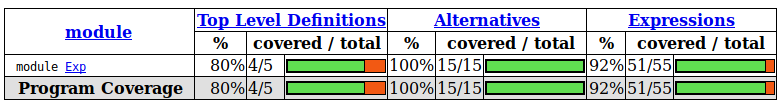
\includegraphics[width=0.95\linewidth]{Images/coverage_exp}
\caption{Test coverage results for the expression language.}
\label{fig:coverage-exp}
\end{figure}

HPC displays information in two different ways: reports with summary statistics (as shown above) and sources with color mark-up (which we will explore in Chapter~\ref{chap:testing}). The information provided in Figure~\ref{fig:coverage-exp} is measured at three different levels: declarations (both top-level and local), alternatives (among several equations or case branches) and expressions (at every level)~\cite{Gill:2007:HPC:1291201.1291203}, showing important information to improve the quality of test cases. In this case, the figure says that 4 of 5 functions (80\%) were reached, all alternatives were covered, and almost all expressions (92\%) were performed during the execution of our tests.

%%%%%%%%%%%%%%%%%%%%%% Begin lhs2TeX definition %%%%%%%%%%%%%%%%%%%%%%%%%%%%%%%%

% Special chars


% Variables


% Keywords


% Functions


% Types


% Constructors


%%%%%%%%%%%%%%%%%%%% End of lhs2TeX definition %%%%%%%%%%%%%%%%%%%%%%%%%%%%%%%%%

\section{Formal Verification}
\label{sec:itp}

Formal verification uses logical methods to establish claims expressed in precise mathematical terms. When combined with an interactive theorem prover, i.e. the use of proof assistants (like Agda, Coq, or Isabelle), the user can check whether these mathematical properties are satisfied, or verify that certain software (or hardware) meets its formal specifications. Having the properties established, proving correctness becomes a form of theorem proving, and its validity is checked by the system. Every claim (lemma or theorem) about the specification should be supported by a proof in a suitable axiomatic foundation. It means that every inference rule and every step of a calculation has to be justified by prior definitions and theorems~\cite{de2015lean}.

In this section, we present the basics of the dependently-typed programming language Agda, which is a system combining a powerful programming language with mechanisms to verify logic properties. After that, we mechanically check the expression language previously presented using two different (and equivalent) styles of formalization, extrinsic and intrinsic, which will be explored deeply in Chapter \ref{chap:proving}. The most important benefit Agda brings us is that the results implemented in the language are correct according to their specifications, and are checked every time by its underlying system.

\subsection{Overview of Agda}

Agda is a dependently-typed functional programming language based on Martin-L\"of intuitionistic type theory~\cite{Lof98}.  Function types and an infinite hierarchy of types of types, \ensuremath{\D{Set}\;\V{\ell}}, where \ensuremath{\V{\ell}} is a natural number, are built-in. Everything else is a user-defined type. The type \ensuremath{\D{Set}}, also known as \ensuremath{\D{Set}_{\D{0}}}, is the type of all ``small'' types, such as \ensuremath{\D{Bool}}, \ensuremath{\D{String}} and \ensuremath{\D{List}\;\D{Bool}}.  The type \ensuremath{\D{Set}_{\D{1}}} is the type of \ensuremath{\D{Set}} and ``others like it'', such as \ensuremath{\D{Set}\;\to \;\D{Bool}}, \ensuremath{\D{String}\;\to \;\D{Set}}, and \ensuremath{\D{Set}\;\to \;\D{Set}}. We have that \ensuremath{\D{Set}\;\V{\ell}} is an element of the type \ensuremath{\D{Set}\;(\V{\ell}\;\F{+}\;\N{1})}, for every $\ell \geq 0$. This stratification of types is used to keep Agda consistent as a logical theory~\cite{Sorensen2006}.

An ordinary (non-dependent) function type is written \ensuremath{\V{A}\;\to \;\V{B}} and a dependent one is written \ensuremath{(\V{x}\;\mathbin{:}\;\V{A})\;\to \;\V{B}}, where type \ensuremath{\V{B}} depends on
\ensuremath{\V{x}}, or \ensuremath{\V{\forall}\;(\V{x}\;\mathbin{:}\;\V{A})\;\to \;\V{B}}. Agda allows the definition of \emph{implicit parameters}, i.e.  parameters whose values can be infered from the context, by surrounding them in curly braces: \ensuremath{\V{\forall}\;\{\mskip1.5mu \V{x}\;\mathbin{:}\;\V{A}\mskip1.5mu\}\;\to \;\V{B}}. To avoid clutter, sometimes we omit implicit arguments from the source code presentation. The reader can safely assume that every free variable in a type is an implicit parameter.

As an example of Agda code, consider the following datatype of natural numbers and length-indexed lists, also known as vectors.

\begin{hscode}\SaveRestoreHook
\column{B}{@{}>{\hspre}l<{\hspost}@{}}%
\column{3}{@{}>{\hspre}l<{\hspost}@{}}%
\column{5}{@{}>{\hspre}l<{\hspost}@{}}%
\column{11}{@{}>{\hspre}l<{\hspost}@{}}%
\column{E}{@{}>{\hspre}l<{\hspost}@{}}%
\>[3]{}\K{data}\;\D{\mathbb{N}}\;\mathbin{:}\;\D{Set}\;\K{where}{}\<[E]%
\\
\>[3]{}\hsindent{2}{}\<[5]%
\>[5]{}\Con{zero}\;{}\<[11]%
\>[11]{}\mathbin{:}\;\D{\mathbb{N}}{}\<[E]%
\\
\>[3]{}\hsindent{2}{}\<[5]%
\>[5]{}\Con{suc}\;{}\<[11]%
\>[11]{}\mathbin{:}\;\D{\mathbb{N}}\;\to \;\D{\mathbb{N}}{}\<[E]%
\\[\blanklineskip]%
\>[3]{}\K{data}\;\D{Vec}\;(\V{A}\;\mathbin{:}\;\D{Set})\;\mathbin{:}\;\D{\mathbb{N}}\;\to \;\D{Set}\;\K{where}{}\<[E]%
\\
\>[3]{}\hsindent{2}{}\<[5]%
\>[5]{}\Con{\lbrack\:\rbrack}\;{}\<[11]%
\>[11]{}\mathbin{:}\;\D{Vec}\;\V{A}\;\Con{zero}{}\<[E]%
\\
\>[3]{}\hsindent{2}{}\<[5]%
\>[5]{}\Con{\_::\_}\;{}\<[11]%
\>[11]{}\mathbin{:}\;\V{\forall}\;\{\mskip1.5mu \V{n}\mskip1.5mu\}\;\to \;\V{A}\;\to \;\D{Vec}\;\V{A}\;\V{n}\;\to \;\D{Vec}\;\V{A}\;(\Con{suc}\;\V{n}){}\<[E]%
\ColumnHook
\end{hscode}\resethooks

Constructor \ensuremath{\Con{\lbrack\:\rbrack}} builds empty vectors. The cons-operator (\ensuremath{\Con{\_::\_}})\footnote{Agda supports the definition of mixfix operators. We can use underscores to mark arguments positions.} inserts a new element in front of a vector of $n$ elements (of type
\ensuremath{\D{Vec}\;\V{A}\;\V{n}}) and returns a value of type \ensuremath{\D{Vec}\;\V{A}\;(\Con{suc}\;\V{n})}. The \ensuremath{\D{Vec}} datatype is an example of a dependent-type, i.e., a type that uses a value (that denotes its length). The usefulness of dependent types can be illustrated with the definition of a safe list head function: \ensuremath{\F{head}} can be defined to accept only non-empty vectors, i.e.,~values of type \ensuremath{\D{Vec}\;\V{A}\;(\Con{suc}\;\V{n})}, which have at least one element.

\begin{hscode}\SaveRestoreHook
\column{B}{@{}>{\hspre}l<{\hspost}@{}}%
\column{3}{@{}>{\hspre}l<{\hspost}@{}}%
\column{E}{@{}>{\hspre}l<{\hspost}@{}}%
\>[3]{}\F{head}\;\mathbin{:}\;\D{Vec}\;\V{A}\;(\Con{suc}\;\V{n})\;\to \;\V{A}{}\<[E]%
\\
\>[3]{}\F{head}\;(\V{x}\;\Con{::}\;\V{xs})\;\mathrel{=}\;\V{x}{}\<[E]%
\ColumnHook
\end{hscode}\resethooks

In \ensuremath{\F{head}}'s definition, the constructor \ensuremath{\Con{\lbrack\:\rbrack}} is not used. The Agda type-checker can figure out, from \ensuremath{\F{head}}'s parameter type, that argument \ensuremath{\Con{\lbrack\:\rbrack}} to \ensuremath{\F{head}} is not type-correct, hence we do not have to give a definition for that case. In Haskell, \ensuremath{\F{head}\;\Con{\lbrack\:\rbrack}} throws an exception instead.

Another useful datatype is the finite type \ensuremath{\D{Fin}}, which is defined in Agda's standard library as:

\begin{hscode}\SaveRestoreHook
\column{B}{@{}>{\hspre}l<{\hspost}@{}}%
\column{3}{@{}>{\hspre}l<{\hspost}@{}}%
\column{5}{@{}>{\hspre}l<{\hspost}@{}}%
\column{11}{@{}>{\hspre}l<{\hspost}@{}}%
\column{E}{@{}>{\hspre}l<{\hspost}@{}}%
\>[3]{}\K{data}\;\D{Fin}\;\mathbin{:}\;\D{\mathbb{N}}\;\to \;\D{Set}\;\K{where}{}\<[E]%
\\
\>[3]{}\hsindent{2}{}\<[5]%
\>[5]{}\Con{zero}\;{}\<[11]%
\>[11]{}\mathbin{:}\;\V{\forall}\;\{\mskip1.5mu \V{n}\mskip1.5mu\}\;\to \;\D{Fin}\;(\Con{suc}\;\V{n}){}\<[E]%
\\
\>[3]{}\hsindent{2}{}\<[5]%
\>[5]{}\Con{suc}\;{}\<[11]%
\>[11]{}\mathbin{:}\;\V{\forall}\;\{\mskip1.5mu \V{n}\mskip1.5mu\}\;\to \;\D{Fin}\;\V{n}\;\to \;\D{Fin}\;(\Con{suc}\;\V{n}){}\<[E]%
\ColumnHook
\end{hscode}\resethooks
  
Note that Agda supports the overloading of data type constructor names. Constructor \ensuremath{\Con{zero}} can refer to type \ensuremath{\D{\mathbb{N}}} or \ensuremath{\D{Fin}}, depending on the context where the name is used. Type \ensuremath{\D{Fin}\;\V{n}} has exactly \ensuremath{\V{n}} inhabitants (elements), i.e., it is isomorphic to the set $\{0,...,n - 1\}$.
An application of such type is to define a safe vector lookup function, which avoids the access of invalid positions.

\begin{hscode}\SaveRestoreHook
\column{B}{@{}>{\hspre}l<{\hspost}@{}}%
\column{3}{@{}>{\hspre}l<{\hspost}@{}}%
\column{E}{@{}>{\hspre}l<{\hspost}@{}}%
\>[3]{}\F{lookup}\;\mathbin{:}\;\V{\forall}\;\{\mskip1.5mu \V{A}\;\V{n}\mskip1.5mu\}\;\to \;\D{Fin}\;\V{n}\;\to \;\D{Vec}\;\V{A}\;\V{n}\;\to \;\V{A}{}\<[E]%
\\
\>[3]{}\F{lookup}\;\Con{zero}\;(\V{x}\;\Con{::}\;\anonymous )\;\mathrel{=}\;\V{x}{}\<[E]%
\\
\>[3]{}\F{lookup}\;(\Con{suc}\;\V{idx})\;(\anonymous \;\Con{::}\;\V{xs})\;\mathrel{=}\;\F{lookup}\;\V{idx}\;\V{xs}{}\<[E]%
\ColumnHook
\end{hscode}\resethooks

Thanks to the propositions-as-types principle\footnote{Also known as Curry-Howard ``isomorphism''~\cite{Sorensen2006}.} we can interpret
types as logical formulas and terms as proofs. An example is the representation of equality as the following Agda type:

\begin{hscode}\SaveRestoreHook
\column{B}{@{}>{\hspre}l<{\hspost}@{}}%
\column{3}{@{}>{\hspre}l<{\hspost}@{}}%
\column{5}{@{}>{\hspre}l<{\hspost}@{}}%
\column{E}{@{}>{\hspre}l<{\hspost}@{}}%
\>[3]{}\K{data}\;\D{\_ \equiv \_}\;\V{\forall}\;\{\mskip1.5mu \V{\ell}\mskip1.5mu\}\;\{\mskip1.5mu \V{A}\;\mathbin{:}\;\D{Set}\;\V{\ell}\mskip1.5mu\}\;(\V{x}\;\mathbin{:}\;\V{A})\;\mathbin{:}\;\V{A}\;\to \;\D{Set}\;\K{where}{}\<[E]%
\\
\>[3]{}\hsindent{2}{}\<[5]%
\>[5]{}\Con{refl}\;\mathbin{:}\;\V{x}\;\D{\equiv}\;\V{x}{}\<[E]%
\ColumnHook
\end{hscode}\resethooks

This type is called propositional equality. It defines that there is a unique evidence for equality, constructor \ensuremath{\Con{refl}} (for reflexivity),
asserting that the only value equal to \ensuremath{\V{x}} is itself. Given a predicate \ensuremath{\V{P}\;\mathbin{:}\;\V{A}\;\to \;\D{Set}} and a vector \ensuremath{\V{xs}}, the type \ensuremath{\D{All}\;\V{P}\;\V{xs}} is used to build proofs that \ensuremath{\V{P}} holds for all elements in \ensuremath{\V{xs}} and it is defined as:

\begin{hscode}\SaveRestoreHook
\column{B}{@{}>{\hspre}l<{\hspost}@{}}%
\column{3}{@{}>{\hspre}l<{\hspost}@{}}%
\column{6}{@{}>{\hspre}l<{\hspost}@{}}%
\column{12}{@{}>{\hspre}l<{\hspost}@{}}%
\column{41}{@{}>{\hspre}l<{\hspost}@{}}%
\column{E}{@{}>{\hspre}l<{\hspost}@{}}%
\>[3]{}\K{data}\;\D{All}\;(\V{P}\;\mathbin{:}\;\V{A}\;\to \;\D{Set})\;\mathbin{:}\;\D{Vec}\;\V{A}\;\V{n}\;\to \;{}\<[41]%
\>[41]{}\D{Set}\;\K{where}{}\<[E]%
\\
\>[3]{}\hsindent{3}{}\<[6]%
\>[6]{}\Con{\lbrack\:\rbrack}\;{}\<[12]%
\>[12]{}\mathbin{:}\;\D{All}\;\V{P}\;\Con{\lbrack\:\rbrack}{}\<[E]%
\\
\>[3]{}\hsindent{3}{}\<[6]%
\>[6]{}\Con{\_::\_}\;{}\<[12]%
\>[12]{}\mathbin{:}\;\V{\forall}\;\{\mskip1.5mu \V{x}\;\V{xs}\mskip1.5mu\}\;\to \;\V{P}\;\V{x}\;\to \;\D{All}\;\V{P}\;\V{xs}\;\to \;\D{All}\;\V{P}\;(\V{x}\;\Con{::}\;\V{xs}){}\<[E]%
\ColumnHook
\end{hscode}\resethooks
   
The first constructor specifies that \ensuremath{\D{All}\;\V{P}} holds for the empty vector and constructor \ensuremath{\Con{\_::\_}} builds a proof of \ensuremath{\D{All}\;\V{P}\;(\V{x}\;\Con{::}\;\V{xs})} from proofs of \ensuremath{\V{P}\;\V{x}} and \ensuremath{\D{All}\;\V{P}\;\V{xs}}. Since this type shares the structure with vectors, some functions on \ensuremath{\D{Vec}} have similar definitions for type \ensuremath{\D{All}}. As an example, consider the function \ensuremath{\F{lookup}}, which extracts a proof of \ensuremath{\V{P}} for the element at position \ensuremath{\V{v}\;\Con{::}\;\D{Fin}\;\V{n}} in a \ensuremath{\D{Vec}}:

\begin{hscode}\SaveRestoreHook
\column{B}{@{}>{\hspre}l<{\hspost}@{}}%
\column{4}{@{}>{\hspre}l<{\hspost}@{}}%
\column{E}{@{}>{\hspre}l<{\hspost}@{}}%
\>[4]{}\F{lookup}\;\mathbin{:}\;\{\mskip1.5mu \V{xs}\;\mathbin{:}\;\D{Vec}\;\V{A}\;\V{n}\mskip1.5mu\}\;\to \;\D{Fin}\;\V{n}\;\to \;\D{All}\;\V{P}\;\V{xs}\;\to \;\V{P}\;\V{x}{}\<[E]%
\\
\>[4]{}\F{lookup}\;\Con{zero}\;(\V{px}\;\Con{::}\;\anonymous )\;\mathrel{=}\;\V{px}{}\<[E]%
\\
\>[4]{}\F{lookup}\;(\Con{suc}\;\V{idx})\;(\anonymous \;\Con{::}\;\V{pxs})\;\mathrel{=}\;\F{lookup}\;\V{idx}\;\V{pxs}{}\<[E]%
\ColumnHook
\end{hscode}\resethooks

An important application of Agda (and dependent-types) is to encode and prove properties about the specification of programming languages. We will discuss next two different forms to formally describe programming languages, achieving an equivalent soundness result.

\subsection{Formalization Styles}

Nowadays, there are two main approaches to formalize and prove type safety for a programming language. In the first one, called \emph{extrinsic}, usually, the syntax, typing, and evaluation rules are described separately, and the common theorems of progress and preservation link the rules to prove type safety. In the second one, called \emph{intrinsic}, the syntax and the typing judgments are expressed as a single definition, thus allowing only the representation of well-typed terms. Using such definition together with a terminating definitional interpreter, which implements the evaluation rules, type-safety is guaranteed by construction.

Next we present the formalization of the expression language presented in the beginning of this chapter. First we give its definition using the most traditional \emph{extrinsic} approach, and then we present an \emph{intrinsic} variant of the same language.

\subsubsection{Extrinsic Formalization}

To formalize a programming language in the extrinsic format, we follow the usual script: first we give the syntax, the semantics and typing rules, and then we prove the properties of progress and preservation to guarantee type-safety.

\vspace{5pt}

\noindent\emph{Syntax definition.} Defining the syntax is similar to what was done in Haskell. We have a datatype \ensuremath{\D{Expr}}, and one constructor for each expressions\footnote{Agda allows inline definitions of constructors resulting on the same type. We can see that for constructor \ensuremath{\Con{True}} and \ensuremath{\Con{False}} with type \ensuremath{\D{Expr}}, and for \ensuremath{\Con{\_\land\_}} and \ensuremath{\Con{\_+\_}} with type \ensuremath{\D{Expr}\;\to \;\D{Expr}\;\to \;\D{Expr}}.}.

\begin{hscode}\SaveRestoreHook
\column{B}{@{}>{\hspre}l<{\hspost}@{}}%
\column{4}{@{}>{\hspre}l<{\hspost}@{}}%
\column{7}{@{}>{\hspre}l<{\hspost}@{}}%
\column{19}{@{}>{\hspre}l<{\hspost}@{}}%
\column{21}{@{}>{\hspre}l<{\hspost}@{}}%
\column{E}{@{}>{\hspre}l<{\hspost}@{}}%
\>[4]{}\K{data}\;\D{Expr}\;\mathbin{:}\;\D{Set}\;\K{where}{}\<[E]%
\\
\>[4]{}\hsindent{3}{}\<[7]%
\>[7]{}\HC{BTrue}\;\HC{BFalse}\;{}\<[21]%
\>[21]{}\mathbin{:}\;\D{Expr}{}\<[E]%
\\
\>[4]{}\hsindent{3}{}\<[7]%
\>[7]{}\Con{Num}\;{}\<[19]%
\>[19]{}\mathbin{:}\;\D{\mathbb{N}}\;\to \;\D{Expr}{}\<[E]%
\\
\>[4]{}\hsindent{3}{}\<[7]%
\>[7]{}\Con{\_\land\_}\;\Con{\_+\_}\;{}\<[19]%
\>[19]{}\mathbin{:}\;\D{Expr}\;\to \;\D{Expr}\;\to \;\D{Expr}{}\<[E]%
\ColumnHook
\end{hscode}\resethooks

The reader can note that, similarly to our Haskell definition (presented earlier), using this datatype we can construct expressions denoting terms that should not be considered well-typed such as \ensuremath{(\Con{Num}\;\N{1})\;\F{+}\;\Con{True}}, but our typing relation will forbid this.

\vspace{8pt}

\noindent\emph{Values.} The presented language has three constructors to define values. Constructors \ensuremath{\Con{VTrue}} and \ensuremath{\Con{VFalse}} say that the boolean constants are values. Constructor \ensuremath{\Con{VNum}} also represents a value giving that \ensuremath{\V{n}} is of type \ensuremath{\D{\mathbb{N}}}.

\pagebreak

\begin{hscode}\SaveRestoreHook
\column{B}{@{}>{\hspre}l<{\hspost}@{}}%
\column{3}{@{}>{\hspre}l<{\hspost}@{}}%
\column{5}{@{}>{\hspre}l<{\hspost}@{}}%
\column{12}{@{}>{\hspre}l<{\hspost}@{}}%
\column{E}{@{}>{\hspre}l<{\hspost}@{}}%
\>[3]{}\K{data}\;\D{Val}\;\mathbin{:}\;\D{Expr}\;\V{\rightarrow}\;\D{Set}\;\K{where}{}\<[E]%
\\
\>[3]{}\hsindent{2}{}\<[5]%
\>[5]{}\Con{VTrue}\;{}\<[12]%
\>[12]{}\mathbin{:}\;\D{Val}\;\HC{BTrue}{}\<[E]%
\\
\>[3]{}\hsindent{2}{}\<[5]%
\>[5]{}\Con{VFalse}\;\mathbin{:}\;\D{Val}\;\HC{BFalse}{}\<[E]%
\\
\>[3]{}\hsindent{2}{}\<[5]%
\>[5]{}\Con{VNum}\;{}\<[12]%
\>[12]{}\mathbin{:}\;\V{\forall}\;\{\mskip1.5mu \V{n}\mskip1.5mu\}\;\V{\rightarrow}\;\D{Val}\;(\Con{Num}\;\V{n}){}\<[E]%
\ColumnHook
\end{hscode}\resethooks

\vspace{-1ex}

The inductive definition \ensuremath{\D{Val}} is indexed by an \ensuremath{\D{Expr}}, showing which syntactical constructor is associated with each value. We need this definition to define the reduction steps.

\vspace{3pt}

\noindent\emph{Dynamic semantics.} The formalization of the evaluation for the expression language using the extrinsic approach follows the small-step semantics presented in Figure~\ref{fig:smallexp}. The Agda code is basically a translation of the presented inference rules. The first three constructors deal with the arithmetic operator, and the last three constructors deal with the boolean operator. We use the \ensuremath{\D{Val}} datatype to force some of the expressions to be values in some rules. Following the same idea of the small-step rules, we rename Agda's addition operator (\ensuremath{\F{+}} to \ensuremath{\F{\oplus}}) to avoid name conflicts. 

\vspace{-1ex}

\begin{hscode}\SaveRestoreHook
\column{B}{@{}>{\hspre}l<{\hspost}@{}}%
\column{3}{@{}>{\hspre}l<{\hspost}@{}}%
\column{5}{@{}>{\hspre}l<{\hspost}@{}}%
\column{13}{@{}>{\hspre}l<{\hspost}@{}}%
\column{E}{@{}>{\hspre}l<{\hspost}@{}}%
\>[3]{}\K{data}\;\F{\_\longrightarrow\_}\;\mathbin{:}\;\D{Expr}\;\V{\rightarrow}\;\D{Expr}\;\V{\rightarrow}\;\D{Set}\;\K{where}{}\<[E]%
\\
\>[3]{}\hsindent{2}{}\<[5]%
\>[5]{}\Con{S\textrm{-}Add_1}\;{}\<[13]%
\>[13]{}\mathbin{:}\;\V{\forall}\;\{\mskip1.5mu \V{e_1}\;\V{e_1'}\;\V{e_2}\mskip1.5mu\}\;{}\<[E]%
\\
\>[13]{}\V{\rightarrow}\;\V{e_1}\;\F{\longrightarrow}\;\V{e_1'}\;{}\<[E]%
\\
\>[13]{}\V{\rightarrow}\;\V{e_1}\;\F{+}\;\V{e_2}\;\F{\longrightarrow}\;\V{e_1'}\;\F{+}\;\V{e_2}{}\<[E]%
\\
\>[3]{}\hsindent{2}{}\<[5]%
\>[5]{}\Con{S\textrm{-}Add_2}\;{}\<[13]%
\>[13]{}\mathbin{:}\;\V{\forall}\;\{\mskip1.5mu \V{v_1}\;\V{e_2}\;\V{e_2'}\mskip1.5mu\}\;{}\<[E]%
\\
\>[13]{}\V{\rightarrow}\;\D{Val}\;\V{v_1}\;{}\<[E]%
\\
\>[13]{}\V{\rightarrow}\;\V{e_2}\;\F{\longrightarrow}\;\V{e_2'}\;{}\<[E]%
\\
\>[13]{}\V{\rightarrow}\;\V{v_1}\;\F{+}\;\V{e_2}\;\F{\longrightarrow}\;\V{v_1}\;\F{+}\;\V{e_2'}{}\<[E]%
\\
\>[3]{}\hsindent{2}{}\<[5]%
\>[5]{}\Con{S\textrm{-}Add}\;{}\<[13]%
\>[13]{}\mathbin{:}\;\V{\forall}\;\{\mskip1.5mu \V{n_1}\;\V{n_2}\mskip1.5mu\}\;{}\<[E]%
\\
\>[13]{}\V{\rightarrow}\;\D{Val}\;(\Con{Num}\;\V{n_1})\;{}\<[E]%
\\
\>[13]{}\V{\rightarrow}\;\D{Val}\;(\Con{Num}\;\V{n_2})\;{}\<[E]%
\\
\>[13]{}\V{\rightarrow}\;(\Con{Num}\;\V{n_1})\;\F{+}\;(\Con{Num}\;\V{n_2})\;\F{\longrightarrow}\;\Con{Num}\;(\V{n_1}\;\F{\oplus}\;\V{n_2}){}\<[E]%
\\
\>[3]{}\hsindent{2}{}\<[5]%
\>[5]{}\Con{S\textrm{-}And_1}\;{}\<[13]%
\>[13]{}\mathbin{:}\;\V{\forall}\;\{\mskip1.5mu \V{e_1}\;\V{e_1'}\;\V{e_2}\mskip1.5mu\}\;{}\<[E]%
\\
\>[13]{}\V{\rightarrow}\;\V{e_1}\;\F{\longrightarrow}\;\V{e_1'}\;{}\<[E]%
\\
\>[13]{}\V{\rightarrow}\;\V{e_1}\;\F{\wedge}\;\V{e_2}\;\F{\longrightarrow}\;\V{e_1'}\;\F{\wedge}\;\V{e_2}{}\<[E]%
\\
\>[3]{}\hsindent{2}{}\<[5]%
\>[5]{}\Con{S\textrm{-}And_2}\;{}\<[13]%
\>[13]{}\mathbin{:}\;\V{\forall}\;\{\mskip1.5mu \V{e_2}\mskip1.5mu\}\;{}\<[E]%
\\
\>[13]{}\V{\rightarrow}\;\D{Val}\;\HC{BTrue}\;{}\<[E]%
\\
\>[13]{}\V{\rightarrow}\;\HC{BTrue}\;\F{\wedge}\;\V{e_2}\;\F{\longrightarrow}\;\V{e_2}{}\<[E]%
\\
\>[3]{}\hsindent{2}{}\<[5]%
\>[5]{}\Con{S\textrm{-}And_3}\;{}\<[13]%
\>[13]{}\mathbin{:}\;\V{\forall}\;\{\mskip1.5mu \V{e_2}\mskip1.5mu\}\;{}\<[E]%
\\
\>[13]{}\V{\rightarrow}\;\D{Val}\;\HC{BFalse}\;{}\<[E]%
\\
\>[13]{}\V{\rightarrow}\;\HC{BFalse}\;\F{\wedge}\;\V{e_2}\;\F{\longrightarrow}\;\HC{BFalse}{}\<[E]%
\ColumnHook
\end{hscode}\resethooks

\vspace{-1ex}

\noindent\emph{Syntax of types.} The present formalization presumes the existence of only two types: \ensuremath{\HC{TBool}} representing booleans, and \ensuremath{\HC{TNum}} representing numbers. 

\begin{hscode}\SaveRestoreHook
\column{B}{@{}>{\hspre}l<{\hspost}@{}}%
\column{3}{@{}>{\hspre}l<{\hspost}@{}}%
\column{E}{@{}>{\hspre}l<{\hspost}@{}}%
\>[B]{}\K{data}\;\D{Ty}\;\mathbin{:}\;\D{Set}\;\K{where}{}\<[E]%
\\
\>[B]{}\hsindent{3}{}\<[3]%
\>[3]{}\HC{TBool}\;\HC{TNum}\;\mathbin{:}\;\D{Ty}{}\<[E]%
\ColumnHook
\end{hscode}\resethooks

\noindent\emph{Expression typing.} The \ensuremath{\F{\vdash\_:\_}} relation encodes the typing rules for the expression language, indicating that an expression \ensuremath{\D{Expr}} has type \ensuremath{\D{Ty}}. Again, the Agda encoding is very similar to the rules presented in Figure~\ref{fig:typing}. First three constructors give types for values \ensuremath{\HC{BTrue}}, \ensuremath{\HC{BFalse}}, and \ensuremath{\Con{Num}}. Constructor \ensuremath{\Con{T\textrm{-}Add}} will have type \ensuremath{\HC{TNum}} giving that both \ensuremath{\V{e_1}} and \ensuremath{\V{e_2}} have type \ensuremath{\HC{TNum}}. Similarly, \ensuremath{\Con{T\textrm{-}And}} has type \ensuremath{\HC{TBool}} if both \ensuremath{\V{e_1}} and \ensuremath{\V{e_2}} have type \ensuremath{\HC{TBool}}.

\begin{hscode}\SaveRestoreHook
\column{B}{@{}>{\hspre}l<{\hspost}@{}}%
\column{3}{@{}>{\hspre}l<{\hspost}@{}}%
\column{5}{@{}>{\hspre}l<{\hspost}@{}}%
\column{13}{@{}>{\hspre}l<{\hspost}@{}}%
\column{E}{@{}>{\hspre}l<{\hspost}@{}}%
\>[3]{}\K{data}\;\F{\vdash\_:\_}\;\mathbin{:}\;\D{Expr}\;\V{\rightarrow}\;\D{Ty}\;\V{\rightarrow}\;\D{Set}\;\K{where}{}\<[E]%
\\
\>[3]{}\hsindent{2}{}\<[5]%
\>[5]{}\Con{T\textrm{-}True}\;{}\<[13]%
\>[13]{}\mathbin{:}\;\F{\vdash}\;\HC{BTrue}\;\F{:}\;\HC{TBool}{}\<[E]%
\\
\>[3]{}\hsindent{2}{}\<[5]%
\>[5]{}\Con{T\textrm{-}False}\;\mathbin{:}\;\F{\vdash}\;\HC{BFalse}\;\F{:}\;\HC{TBool}{}\<[E]%
\\
\>[3]{}\hsindent{2}{}\<[5]%
\>[5]{}\Con{T\textrm{-}Num}\;{}\<[13]%
\>[13]{}\mathbin{:}\;\V{\forall}\;\{\mskip1.5mu \V{n}\mskip1.5mu\}\;\V{\rightarrow}\;\F{\vdash}\;\Con{Num}\;\V{n}\;\F{:}\;\HC{TNum}{}\<[E]%
\\
\>[3]{}\hsindent{2}{}\<[5]%
\>[5]{}\Con{T\textrm{-}Add}\;{}\<[13]%
\>[13]{}\mathbin{:}\;\V{\forall}\;\{\mskip1.5mu \V{e_1}\;\V{e_2}\mskip1.5mu\}\;{}\<[E]%
\\
\>[13]{}\V{\rightarrow}\;\F{\vdash}\;\V{e_1}\;\F{:}\;\HC{TNum}\;{}\<[E]%
\\
\>[13]{}\V{\rightarrow}\;\F{\vdash}\;\V{e_2}\;\F{:}\;\HC{TNum}\;{}\<[E]%
\\
\>[13]{}\V{\rightarrow}\;\F{\vdash}\;\V{e_1}\;\F{+}\;\V{e_2}\;\F{:}\;\HC{TNum}{}\<[E]%
\\
\>[3]{}\hsindent{2}{}\<[5]%
\>[5]{}\Con{T\textrm{-}And}\;{}\<[13]%
\>[13]{}\mathbin{:}\;\V{\forall}\;\{\mskip1.5mu \V{e_1}\;\V{e_2}\mskip1.5mu\}\;{}\<[E]%
\\
\>[13]{}\V{\rightarrow}\;\F{\vdash}\;\V{e_1}\;\F{:}\;\HC{TBool}\;{}\<[E]%
\\
\>[13]{}\V{\rightarrow}\;\F{\vdash}\;\V{e_2}\;\F{:}\;\HC{TBool}\;{}\<[E]%
\\
\>[13]{}\V{\rightarrow}\;\F{\vdash}\;\V{e_1}\;\F{\wedge}\;\V{e_2}\;\F{:}\;\HC{TBool}{}\<[E]%
\ColumnHook
\end{hscode}\resethooks

Expressions obeying the rules expressed in this relation are considered well-typed, otherwise they are said to be ill-typed.

\vspace{5pt}

\noindent\emph{Soundness proofs.} We now prove type soundness for the language tested before with QuickCheck using the extrinsic approach. 

First we need to define formally the basic property of reduction and types, identifying the possible \emph{canonical forms} (i.e., well-typed closed values) belonging to each type~\cite{pierce2019software}. The definition has one constructor for each value (\ensuremath{\Con{C\textrm{-}True}}, \ensuremath{\Con{C\textrm{-}False}}, and \ensuremath{\Con{C\textrm{-}Num}}). 

\begin{hscode}\SaveRestoreHook
\column{B}{@{}>{\hspre}l<{\hspost}@{}}%
\column{3}{@{}>{\hspre}l<{\hspost}@{}}%
\column{5}{@{}>{\hspre}l<{\hspost}@{}}%
\column{13}{@{}>{\hspre}l<{\hspost}@{}}%
\column{E}{@{}>{\hspre}l<{\hspost}@{}}%
\>[3]{}\K{data}\;\D{Canonical}\;\mathbin{:}\;\D{Expr}\;\V{\rightarrow}\;\D{Ty}\;\V{\rightarrow}\;\D{Set}\;\K{where}{}\<[E]%
\\
\>[3]{}\hsindent{2}{}\<[5]%
\>[5]{}\Con{C\textrm{-}True}\;{}\<[13]%
\>[13]{}\mathbin{:}\;\D{Canonical}\;\HC{BTrue}\;\HC{TBool}{}\<[E]%
\\
\>[3]{}\hsindent{2}{}\<[5]%
\>[5]{}\Con{C\textrm{-}False}\;\mathbin{:}\;\D{Canonical}\;\HC{BFalse}\;\HC{TBool}{}\<[E]%
\\
\>[3]{}\hsindent{2}{}\<[5]%
\>[5]{}\Con{C\textrm{-}Num}\;{}\<[13]%
\>[13]{}\mathbin{:}\;\V{\forall}\;\{\mskip1.5mu \V{n}\mskip1.5mu\}\;\V{\rightarrow}\;\D{Canonical}\;(\Con{Num}\;\V{n})\;\HC{TNum}{}\<[E]%
\ColumnHook
\end{hscode}\resethooks

And a proof linking each value with its respective type.

\begin{hscode}\SaveRestoreHook
\column{B}{@{}>{\hspre}l<{\hspost}@{}}%
\column{3}{@{}>{\hspre}l<{\hspost}@{}}%
\column{E}{@{}>{\hspre}l<{\hspost}@{}}%
\>[3]{}\F{canonical}\;\mathbin{:}\;\V{\forall}\;\{\mskip1.5mu \V{v}\;\V{\tau}\mskip1.5mu\}\;\V{\rightarrow}\;\F{\vdash}\;\V{v}\;\F{:}\;\V{\tau}\;\V{\rightarrow}\;\D{Val}\;\V{v}\;\V{\rightarrow}\;\D{Canonical}\;\V{v}\;\V{\tau}{}\<[E]%
\\
\>[3]{}\F{canonical}\;\Con{T\textrm{-}True}\;\anonymous \;\mathrel{=}\;\Con{C\textrm{-}True}{}\<[E]%
\\
\>[3]{}\F{canonical}\;\Con{T\textrm{-}False}\;\anonymous \;\mathrel{=}\;\Con{C\textrm{-}False}{}\<[E]%
\\
\>[3]{}\F{canonical}\;\Con{T\textrm{-}Num}\;\anonymous \;\mathrel{=}\;\Con{C\textrm{-}Num}{}\<[E]%
\ColumnHook
\end{hscode}\resethooks

The \ensuremath{\F{progress}} function represents the theorem with the same name presented earlier, stating that if a well-typed expression \ensuremath{\V{e}} has type \ensuremath{\V{\tau}}, then it can make \emph{Progress}, i.e., or \ensuremath{\V{e}} is a value, or it can take another reduction step. Before giving the proof, we define an inductive datatype to hold the result of our proof, with two constructors: \ensuremath{\Con{Done}} when \ensuremath{\V{e}} is a value, and \ensuremath{\Con{Step}} when \ensuremath{\V{e}} reduces to an \ensuremath{\V{e'}}\footnote{For clarity, we use the definition of a \ensuremath{\D{Progress}} datatype, following the ideas presented in Wadler's book~\cite{Wadler-plfa}. We could achieve similar result using a disjunction operator.}. 

\begin{hscode}\SaveRestoreHook
\column{B}{@{}>{\hspre}l<{\hspost}@{}}%
\column{3}{@{}>{\hspre}l<{\hspost}@{}}%
\column{5}{@{}>{\hspre}l<{\hspost}@{}}%
\column{9}{@{}>{\hspre}l<{\hspost}@{}}%
\column{E}{@{}>{\hspre}l<{\hspost}@{}}%
\>[3]{}\K{data}\;\D{Progress}\;(\V{e}\;\mathbin{:}\;\D{Expr})\;\mathbin{:}\;\D{Set}\;\K{where}{}\<[E]%
\\
\>[3]{}\hsindent{2}{}\<[5]%
\>[5]{}\Con{Step}\;\mathbin{:}\;\V{\forall}\;\{\mskip1.5mu \V{e'}\mskip1.5mu\}\;{}\<[E]%
\\
\>[5]{}\hsindent{4}{}\<[9]%
\>[9]{}\V{\rightarrow}\;\V{e}\;\F{\longrightarrow}\;\V{e'}\;{}\<[E]%
\\
\>[5]{}\hsindent{4}{}\<[9]%
\>[9]{}\V{\rightarrow}\;\D{Progress}\;\V{e}{}\<[E]%
\\
\>[3]{}\hsindent{2}{}\<[5]%
\>[5]{}\Con{Done}\;\mathbin{:}\;\D{Val}\;\V{e}\;{}\<[E]%
\\
\>[5]{}\hsindent{4}{}\<[9]%
\>[9]{}\V{\rightarrow}\;\D{Progress}\;\V{e}{}\<[E]%
\ColumnHook
\end{hscode}\resethooks

The proof of \emph{progress} for this language in Agda is straightforward: cases with values are finished with \ensuremath{\Con{Done}}, and the respective \ensuremath{\D{Val}} constructor; the case for \ensuremath{\Con{T\textrm{-}Add}} makes progress (applying the induction hypothesis) for \ensuremath{\V{e_1}} and \ensuremath{\V{e_2}} and finishes with the canonical values and the rule \ensuremath{\Con{S\textrm{-}Add}}; and the case for \ensuremath{\Con{T\textrm{-}And}} makes progress for \ensuremath{\V{e_1}}, finishing the proof with the rules \ensuremath{\Con{S\textrm{-}And_2}} or \ensuremath{\Con{S\textrm{-}And_3}} according to the respective canonical value\footnote{The `...' notation is used when the original arguments for the \ensuremath{\K{with}} constructor are the same in the new clauses.}.

\begin{hscode}\SaveRestoreHook
\column{B}{@{}>{\hspre}l<{\hspost}@{}}%
\column{3}{@{}>{\hspre}l<{\hspost}@{}}%
\column{9}{@{}>{\hspre}l<{\hspost}@{}}%
\column{11}{@{}>{\hspre}l<{\hspost}@{}}%
\column{E}{@{}>{\hspre}l<{\hspost}@{}}%
\>[3]{}\F{progress}\;\mathbin{:}\;\V{\forall}\;\{\mskip1.5mu \V{e}\;\V{\tau}\mskip1.5mu\}\;\V{\rightarrow}\;\F{\vdash}\;\V{e}\;\F{:}\;\V{\tau}\;\V{\rightarrow}\;\D{Progress}\;\V{e}{}\<[E]%
\\
\>[3]{}\F{progress}\;\Con{T\textrm{-}True}\;\mathrel{=}\;\Con{Done}\;\Con{VTrue}{}\<[E]%
\\
\>[3]{}\F{progress}\;\Con{T\textrm{-}False}\;\mathrel{=}\;\Con{Done}\;\Con{VFalse}{}\<[E]%
\\
\>[3]{}\F{progress}\;\Con{T\textrm{-}Num}\;\mathrel{=}\;\Con{Done}\;\Con{VNum}{}\<[E]%
\\
\>[3]{}\F{progress}\;(\Con{T\textrm{-}Add}\;\V{e_1}\;\V{e_2})\;\K{with}\;\F{progress}\;\V{e_1}{}\<[E]%
\\
\>[3]{}\V{...}\;\mid \;\Con{Step}\;\V{stp_1}\;\mathrel{=}\;\Con{Step}\;(\Con{S\textrm{-}Add_1}\;\V{stp_1}){}\<[E]%
\\
\>[3]{}\V{...}\;\mid \;\Con{Done}\;\V{v_1}\;\K{with}\;\F{progress}\;\V{e_2}{}\<[E]%
\\
\>[3]{}\V{...}\;{}\<[9]%
\>[9]{}\mid \;\Con{Step}\;\V{stp_2}\;\mathrel{=}\;\Con{Step}\;(\Con{S\textrm{-}Add_2}\;\V{v_1}\;\V{stp_2}){}\<[E]%
\\
\>[3]{}\V{...}\;{}\<[9]%
\>[9]{}\mid \;\Con{Done}\;\V{v_2}\;\K{with}\;\F{canonical}\;\V{e_1}\;\V{v_1}\;\mid \;\F{canonical}\;\V{e_2}\;\V{v_2}{}\<[E]%
\\
\>[3]{}\V{...}\;{}\<[11]%
\>[11]{}\mid \;\Con{C\textrm{-}Num}\;\mid \;\Con{C\textrm{-}Num}\;\mathrel{=}\;\Con{Step}\;(\Con{S\textrm{-}Add}\;\V{v_1}\;\V{v_2}){}\<[E]%
\\
\>[3]{}\F{progress}\;(\Con{T\textrm{-}And}\;\V{e_1}\;\V{e_2})\;\K{with}\;\F{progress}\;\V{e_1}{}\<[E]%
\\
\>[3]{}\V{...}\;\mid \;\Con{Step}\;\V{stp_1}\;\mathrel{=}\;\Con{Step}\;(\Con{S\textrm{-}And_1}\;\V{stp_1}){}\<[E]%
\\
\>[3]{}\V{...}\;\mid \;\Con{Done}\;\V{v_1}\;\K{with}\;\F{canonical}\;\V{e_1}\;\V{v_1}{}\<[E]%
\\
\>[3]{}\V{...}\;{}\<[9]%
\>[9]{}\mid \;\Con{C\textrm{-}True}\;\mathrel{=}\;\Con{Step}\;(\Con{S\textrm{-}And_2}\;\V{v_1}){}\<[E]%
\\
\>[3]{}\V{...}\;{}\<[9]%
\>[9]{}\mid \;\Con{C\textrm{-}False}\;\mathrel{=}\;\Con{Step}\;(\Con{S\textrm{-}And_3}\;\V{v_1}){}\<[E]%
\ColumnHook
\end{hscode}\resethooks

The \ensuremath{\F{preservation}} function also represents the theorem with the same name presented earlier, stating that if a well-typed expression \ensuremath{\V{e}} has type \ensuremath{\V{\tau}}, and it takes a reduction step \ensuremath{\V{e}\;\F{\longrightarrow}\;\V{e'}}, then \ensuremath{\V{e'}} remains with type \ensuremath{\V{\tau}}. The proof proceeds by induction on the typing relation, case splitting each reduction case. First three cases deal with the arithmetic operator, and the last three cases deal with the boolean operator. The reader can note that the Agda system is smart enough to figure out that it is not necessary to deal with values, since they cannot take any reduction step. 

\begin{hscode}\SaveRestoreHook
\column{B}{@{}>{\hspre}l<{\hspost}@{}}%
\column{3}{@{}>{\hspre}l<{\hspost}@{}}%
\column{E}{@{}>{\hspre}l<{\hspost}@{}}%
\>[3]{}\F{preservation}\;\mathbin{:}\;\V{\forall}\;\{\mskip1.5mu \V{e}\;\V{e'}\;\V{\tau}\mskip1.5mu\}\;\V{\rightarrow}\;\F{\vdash}\;\V{e}\;\F{:}\;\V{\tau}\;\V{\rightarrow}\;\V{e}\;\F{\longrightarrow}\;\V{e'}\;\V{\rightarrow}\;\F{\vdash}\;\V{e'}\;\F{:}\;\V{\tau}{}\<[E]%
\\
\>[3]{}\F{preservation}\;(\Con{T\textrm{-}Add}\;\V{r_1}\;\V{r_2})\;(\Con{S\textrm{-}Add_1}\;\V{stp})\;\mathrel{=}\;\Con{T\textrm{-}Add}\;(\F{preservation}\;\V{r_1}\;\V{stp})\;\V{r_2}{}\<[E]%
\\
\>[3]{}\F{preservation}\;(\Con{T\textrm{-}Add}\;\V{r_1}\;\V{r_2})\;(\Con{S\textrm{-}Add_2}\;\V{v_1}\;\V{stp})\;\mathrel{=}\;\Con{T\textrm{-}Add}\;\V{r_1}\;(\F{preservation}\;\V{r_2}\;\V{stp}){}\<[E]%
\\
\>[3]{}\F{preservation}\;(\Con{T\textrm{-}Add}\;\V{r_1}\;\V{r_2})\;(\Con{S\textrm{-}Add}\;\V{v_1}\;\V{v_2})\;\mathrel{=}\;\Con{T\textrm{-}Num}{}\<[E]%
\\
\>[3]{}\F{preservation}\;(\Con{T\textrm{-}And}\;\V{r_1}\;\V{r_2})\;(\Con{S\textrm{-}And_1}\;\V{stp})\;\mathrel{=}\;\Con{T\textrm{-}And}\;(\F{preservation}\;\V{r_1}\;\V{stp})\;\V{r_2}{}\<[E]%
\\
\>[3]{}\F{preservation}\;(\Con{T\textrm{-}And}\;\V{r_1}\;\V{r_2})\;(\Con{S\textrm{-}And_2}\;\V{v_1})\;\mathrel{=}\;\V{r_2}{}\<[E]%
\\
\>[3]{}\F{preservation}\;(\Con{T\textrm{-}And}\;\V{r_1}\;\V{r_2})\;(\Con{S\textrm{-}And_3}\;\V{v_1})\;\mathrel{=}\;\V{r_1}{}\<[E]%
\ColumnHook
\end{hscode}\resethooks

\subsubsection{Intrinsic Formalization}

Another possibility to formalize a programming language is to define an intrinsically-typed syntax, combining both the syntax and the typing rules in a single relation, and to define a definitional interpreter, also known as functional big-step semantics, to define its evaluation. Using this approach, we can use dependent-types and the well-behaved features of the host language (Agda) to state soundness of the target language we are working on.

\vspace{5pt}

\noindent\emph{Intrinsically-typed syntax.} Representing the typing rules combined with the language syntax is a well-known approach~\cite{Altenkirch:1999:MPL:647849.737066}. Using such approach, only well-typed expressions are accepted by the host language, and ill-typed expressions are rejected by the compiler accusing type error. Considering this, the abstract syntax trees capture not only the syntactic properties of the language, but semantic properties as well, allowing programmers to reason about their programs as they write them rather than separately at the meta-logical level.

Now, the definition of expressions \ensuremath{\D{Expr}} is parameterized by a type \ensuremath{\D{Ty}} (the same presented for the extrinsic approach).

\begin{hscode}\SaveRestoreHook
\column{B}{@{}>{\hspre}l<{\hspost}@{}}%
\column{4}{@{}>{\hspre}l<{\hspost}@{}}%
\column{7}{@{}>{\hspre}l<{\hspost}@{}}%
\column{E}{@{}>{\hspre}l<{\hspost}@{}}%
\>[4]{}\K{data}\;\D{Expr}\;\mathbin{:}\;\D{Ty}\;\to \;\D{Set}\;\K{where}{}\<[E]%
\\
\>[4]{}\hsindent{3}{}\<[7]%
\>[7]{}\Con{True}\;\Con{False}\;\mathbin{:}\;\D{Expr}\;\Con{Bool}{}\<[E]%
\\
\>[4]{}\hsindent{3}{}\<[7]%
\>[7]{}\Con{Num}\;\mathbin{:}\;\Con{Nat}\;\to \;\D{Expr}\;\Con{Nat}{}\<[E]%
\\
\>[4]{}\hsindent{3}{}\<[7]%
\>[7]{}\Con{\_+\_}\;\mathbin{:}\;\D{Expr}\;\Con{Nat}\;\to \;\D{Expr}\;\Con{Nat}\;\to \;\D{Expr}\;\Con{Nat}{}\<[E]%
\\
\>[4]{}\hsindent{3}{}\<[7]%
\>[7]{}\Con{\_\land\_}\;\mathbin{:}\;\D{Expr}\;\Con{Bool}\;\to \;\D{Expr}\;\Con{Bool}\;\to \;\D{Expr}\;\Con{Bool}{}\<[E]%
\ColumnHook
\end{hscode}\resethooks

In this definition, the \ensuremath{\D{Expr}} datatype carries out information about the type of each expression being built. For example, the first two constructor lines define the value expressions with their types. And the last two lines define the operators present in our language. We can note that for these operators, the intrinsically-typed syntax defines the expected type for each (left and right-hand side) expression. This way, Agda's type system can enforce that only well-typed terms could be written. A definition which uses the expression \ensuremath{(\Con{Num}\;\N{1})\;\F{+}\;\Con{True}} will be rejected by Agda's type checker automatically.

\vspace{5pt}

\noindent\emph{Definition of values.} In order to define our interpreter we need a way to define an intrinsically-typed value. We define the datatype \ensuremath{\D{Val}} indexed by a \ensuremath{\D{Ty}}. By using this definition, when interpreting the code, the produced results are converted to an Agda type (host language semantics). Thus, if the value represents a \ensuremath{\HC{TBool}}, it results in the Agda's \ensuremath{\D{Bool}} type. Similarly, \ensuremath{\HC{TNum}} results in a natural number.

\begin{hscode}\SaveRestoreHook
\column{B}{@{}>{\hspre}l<{\hspost}@{}}%
\column{3}{@{}>{\hspre}l<{\hspost}@{}}%
\column{E}{@{}>{\hspre}l<{\hspost}@{}}%
\>[3]{}\D{Val}\;\mathbin{:}\;\D{Ty}\;\V{\rightarrow}\;\D{Set}{}\<[E]%
\\
\>[3]{}\D{Val}\;\HC{TBool}\;\mathrel{=}\;\D{Bool}{}\<[E]%
\\
\>[3]{}\D{Val}\;\HC{TNum}\;\mathrel{=}\;\D{\mathbb{N}}{}\<[E]%
\ColumnHook
\end{hscode}\resethooks

\vspace{5pt}

\noindent\emph{Definitional interpreter.} Next we present a fairly standard definition of an interpreter for the studied language in Agda. Basically, what we do is to use the host language structure to evaluate the target language, implementing the big-step semantics presented in Figure~\ref{fig:bigexp}. The three first defining equations are considering the evaluation of values in the target language, resulting in values in the Agda language. The case for \ensuremath{\HC{Add}}, both side expressions (\ensuremath{\V{e_1}} and \ensuremath{\V{e_2}}) are evaluated at once, then summing up their results with \ensuremath{\F{\oplus}} operator. The process is similar to deal with booleans. The considerate reader can notice that the treatment of \ensuremath{\HC{And}} differs from the big-step semantics. In our implementation we chose to let Agda evaluate booleans using its standard library definition. Again here, we rename the operators (\ensuremath{\F{+}} to \ensuremath{\F{\oplus}}, and \ensuremath{\F{\wedge}} to \ensuremath{\F{\&\&}}) to avoid name conflicts.

\begin{hscode}\SaveRestoreHook
\column{B}{@{}>{\hspre}l<{\hspost}@{}}%
\column{3}{@{}>{\hspre}l<{\hspost}@{}}%
\column{E}{@{}>{\hspre}l<{\hspost}@{}}%
\>[3]{}\F{eval}\;\mathbin{:}\;\V{\forall}\;\{\mskip1.5mu \V{\tau}\mskip1.5mu\}\;\V{\rightarrow}\;\D{Expr}\;\V{\tau}\;\V{\rightarrow}\;\D{Val}\;\V{\tau}{}\<[E]%
\\
\>[3]{}\F{eval}\;\HC{BTrue}\;\mathrel{=}\;\Con{true}{}\<[E]%
\\
\>[3]{}\F{eval}\;\HC{BFalse}\;\mathrel{=}\;\Con{false}{}\<[E]%
\\
\>[3]{}\F{eval}\;(\Con{Num}\;\V{x})\;\mathrel{=}\;\V{x}{}\<[E]%
\\
\>[3]{}\F{eval}\;(\HC{Add}\;\V{e_1}\;\V{e_2})\;\mathrel{=}\;\F{eval}\;\V{e_1}\;\F{\oplus}\;\F{eval}\;\V{e_2}{}\<[E]%
\\
\>[3]{}\F{eval}\;(\HC{And}\;\V{e_1}\;\V{e_2})\;\mathrel{=}\;\F{eval}\;\V{e_1}\;\F{\&\&}\;\F{eval}\;\V{e_2}{}\<[E]%
\ColumnHook
\end{hscode}\resethooks

There are two points to highlight on the intrinsic approach. First, we can note that we do not have any error treatment in our interpreter. This is happening because we are working only with a (intrinsically) well-typed expression, so in this case, the sub-expression types are guaranteed by construction by Agda's type checker. Second, by allowing only the representation of well-typed expressions, the \emph{preservation} property is also assured by construction (the compiler checks that the two \ensuremath{\V{\tau}}'s in the function definition match), and by writing such evaluator in a total language like Agda, the \emph{progress} property is consequently guaranteed.

For further information about Agda, see~\cite{Norell2009,Stump2016,Wadler-plfa}.

\section{Chapter's Final Remarks}

In this chapter we have set the basic script for the rest of this thesis, by reviewing the basic ideas of operational semantics, property-based testing, and formal verification. We equipped this chapter with a basic language serving as example for setting the ground for all aspects we will work in the next chapters. We shall refer later to the examples presented here, to explain most advanced concepts involving property-based testing or formal verification of programming languages. 

%%%%%%%%%%%%%%%%%%%%%% Begin lhs2TeX definition %%%%%%%%%%%%%%%%%%%%%%%%%%%%%%%%

% Java Keywords


% Java Classes


% Java Methods


% Java special formatting


%%%%%%%%%%%%%%%%%%%% End of lhs2TeX definition %%%%%%%%%%%%%%%%%%%%%%%%%%%%%%%%%

\chapter{Target Languages}
\label{chap:target}

In this chapter we bring an overview of the languages we considered during our research about programming language subsets. We start with a classic programming language ($\lambda$-calculus), which is widely used to study concepts of the functional paradigm, to develop the techniques presented in this thesis. After that, we conduct a research to find a subset of a modern object-oriented calculus, considering the Java language, which is one of the most used programming language nowadays. We present a comparison among the formalizations and the criteria to choose the one to explore in depth the techniques discussed in this work.

\section{Functional Subsets}

In this section we study one of the most famous example of programming languages (at least in research circles), the $\lambda$-calculus. It is a well-known purely functional core calculus proposed by Church in 1932~\cite{Church32} capable of expressing computation with only three syntactic constructors: variables, abstractions, and application. The $\lambda$-calculus is a universal model of computation equivalent to Turing machines, and serves as basis for most of the current functional programming languages. Roughly, this calculus consists of constructing lambda expressions and performing reductions operations on them, through function abstraction and application using variable binding and substitution~\cite{Wadler-plfa}.

Here we present a variant of $\lambda$-calculus, called simply-typed lambda calculus (STLC), which consists of the same base language augmented with types. We discuss the introduction of base types, presenting the syntax, semantics, and type system for this small calculus. For a thorough introduction of the $\lambda$-calculus, the reader is directed to~\cite{Hindley:2008:LCI:1388400,Barendregt:1993:LCT:162552.162561}. The goal of this section is to provide a minimal understanding of STLC, which will be referred in other parts of this thesis when implementing the studied techniques.

\subsection{Simply-Typed Lambda Calculus}

Pure $\lambda$-calculus has only three syntactic constructors. For simplicity, we augment the pure calculus with the boolean constants $true$ and $false$. The abstract syntax of STLC is defined in Figure~\ref{fig:syntax-stlc}. Besides constants, we have \emph{variables}, function definition through \emph{abstraction}, and function invocation with \emph{application}. In the same figure, we also define an \emph{abstraction} as a value for the STLC language, plus the two boolean constants. Similarly to the previous chapter, we use meta-variables $e$ and $v$ to range over expressions and values, following the same conventions. Here, we also let $x$, $y$, and $z$ denote variables. 

\begin{figure}[!htb]
\[
\begin{array}{llr}
  e ::= & \ \ \ \ \ \ \ \ \ \ \ \ \ \ \ \ \ \ \ \ \ \ \ \ \ \ \ \ \ \ \ \ \ \ \ \ \ \  & \textrm{expressions: } \\
        & true & \textrm{constant true} \\
        & false & \textrm{constant false} \\
        & x & \textrm{variable} \\
        & \lambda x . e & \textrm{abstraction} \\
        & e ~ e & \textrm{application} \\
  v ::= & & \textrm{values:} \\
        & true & \textrm{true value} \\
        & false & \textrm{false value} \\
        & \lambda x . e & \textrm{abstraction value} \\
\end{array}
\]
\caption{Abstract syntax for STLC.}
\label{fig:syntax-stlc}
\end{figure}

\vspace{-1ex}

Suppose we have a $\lambda$-expression $\lambda y . (\lambda z . x (y ~ z))$. We say that $y$ and $z$ are bound variables and $x$ is a free variable (as there is no visible abstraction binding it). This notion is important to clarify the \emph{scope} of variables. For this calculus, we assume Barendregt's variable convention, which says that expressions do not have any name clashing. 

The most important notion of $\lambda$-calculus (and consequently STLC) is \emph{substitution} to define how to compute an expression. The computation is given by the \emph{application} of functions to arguments (which themselves can be functions). Each step in the computation consists of rewriting an application whose left-hand side is an \emph{abstraction}, substituting the right-hand side for the bound variable in the abstraction's body~\cite{Pierce:2002:TPL:509043}. We will write $(\lambda x . e_1) e_2 --> \lbrack x \mapsto e_2 \rbrack e_1$, where $\lbrack x \mapsto e_2 \rbrack e_1$ means ``the expression obtained by replacing all free occurrences of $x$ in $e_1$ by $e_2$''. The substitution operation is defined inductively in Figure~\ref{fig:subs-stlc}.

\begin{figure}[!htb]
\[
\begin{array}{lcll}
  \lbrack x \mapsto s \rbrack x                 & = & s                                        &  \\
  \lbrack x \mapsto s \rbrack y                 & = & y                                        & \textrm{if} ~ x \neq y \\
  \lbrack x \mapsto s \lbrack (\lambda y . e_1) & = & \lambda y . [x \mapsto s] e_1            &  \\
  \lbrack x \mapsto s \rbrack (e_1 ~ e_2)       & = & ([x \mapsto s] e_1) ~ ([x \mapsto s] e_2) &  \\
\end{array}
\]
\caption{Variable substitution operation.}
\label{fig:subs-stlc}
\end{figure}

An expression of the form $(\lambda x . e_1) e_2$ is called a \emph{redex}, i.e., a reducible expression, and the operation of rewriting a redex is called \emph{beta-reduction}. Several different reduction strategies can be applied to $\lambda$-calculus (such as \emph{call-by-value}, \emph{call-by-name}, etc.), defining which redex (or redexes) should be reduced on the next step of evaluation.

We present the small-step semantics for STLC in Figure~\ref{fig:small-stlc}. Rule {\footnotesize S-App$_1$} and {\footnotesize S-App$_2$} are \emph{congruence} rules (call-by-value), where the first evaluates the expression on the left of a function application, while the second evaluates the expression on the right, once the first is a value. Rule {\footnotesize S-AppAbs} uses the substitution operation to perform the actual computation, substituting all free occurrences of $x$ on the $\lambda$-expression body $e_1$. The reader can note that we are presenting a \emph{call-by-value} evaluation strategy, since we are only applying the substitution if the right expression is a value ($v_2$). 

\begin{figure}[!htb]
\[
\begin{array}{ccc}    
  \inference{e_1 --> e_1'}
            {e_1 ~ e_2 --> e_1' ~ e_2}[\textrm{[S-App$_1$]}]
& &
  \inference{e_2 --> e_2'}
            {v_1 ~ e_2 --> v_1 ~ e_2'}[\textrm{[S-App$_2$]}]
\end{array}    
\]
\vspace{3pt}
\[
\begin{array}{ccc}
  & (\lambda x . e_1) v_2 --> \lbrack x \mapsto v_2 \rbrack e_1 \ \ \footnotesize\textrm{[S-AppAbs]} &
\end{array}    
\]
\caption{Small-step semantics for STLC.}
\label{fig:small-stlc}
\end{figure}

In order to define the type system for STLC, first we define the set of types in Figure~\ref{fig:types-stlc}. % Using this definition, we can have type $Bool$, $Bool -> Bool$, $Bool -> Bool -> Bool$, and so on. For example, $Bool -> Bool$ represents a function taking a $Bool$ as parameter, and returning a value of type $Bool$.

\begin{figure}[!htb]
\[
\begin{array}{llr}
  T ::= & \ \ \ \ \ \ \ \ \ \ \ \ \ \ \ \ \ \ \ \ \ \ \ \ \ \ \ \ \ \ \ \ \ \ \ \ \ \ & \textrm{types: } \\
        & Bool  & \textrm{type of booleans} \\
        & T -> T & \textrm{type of functions} \\
\end{array}
\]
\caption{Simple types for STLC.}
\label{fig:types-stlc}
\end{figure}

Type-checking in STLC can be carried out structurally. Expressions (on the language we are studying) can have boolean or function types. However, when analyzing $\lambda$-expressions of the form $(\lambda x . e_1) ~ e_2$, the type which should be assigned to the whole program depends on that assigned to the expression $e_2$ according to the form of expression body $e_1$. This dependency can be expressed in terms of assumptions about the free variable $x$ occurring in $e_1$, according to the type assigned to $e_2$. The standard procedure is to define a context $\Gamma$ as a type environment, to hold the association of variables and types. Having this setting, a typing rule is expressed as $\Gamma \vdash e : T$, stating that $e$ has type $T$ according to variables in the $\Gamma$ context. Figure~\ref{fig:look-stlc} presents the definition of the type environment and the lookup operations~\cite{Wadler-plfa}.

\begin{figure}[!htb]
\[
\begin{array}{llr}
  \Gamma ::= & \ \ \ \ \ \ \ \ \ \ \ \ \ \ \ \ \ \ \ \ \ \ \ \ \ \ \ \ \ \ \ \ \ \ \ \ \ \ & \textrm{contexts:} \\
        & \varnothing & \textrm{empty context} \\
        & \Gamma , x : T & \textrm{variable binding} \\           
\end{array}
\]
\[
\begin{array}{ccc}
    \Gamma , x : T \vdash x : T \ \ \footnotesize\textrm{[E-Lkp$_1$]}
  & &
    \inference{\Gamma \vdash x_2 : T_2 \ \ \ \ x_1 \neq x_2}
              {\Gamma , x_1 : T_1 \vdash x_2 : T_2}[\textrm{[E-Lkp$_2$]}]
\end{array}    
\]
\caption{Environment definition and operations.}
\label{fig:look-stlc}
\end{figure}

In this figure, $\varnothing$ represents an empty context (we can see the context as a list), and $\Gamma , x : T$ represents the operation of extending a typing environment with variable $x$ having type $T$. We also use next $dom(\Gamma)$ to denote the set of variables in the domain of context $\Gamma$. Rule {\footnotesize E-Lkp$_1$} is the base case, when the variable appears in the current scanning position, and rule {\footnotesize E-Lkp$_2$} is the recursive case, looking up further on the list, when the variable is different from the one being sought.

Figure \ref{fig:typing-stlc} summarizes the typing judgment rules for STLC. Rules {\footnotesize T-True} and {\footnotesize T-False} define the type for the boolean constants. Rule {\footnotesize T-Var} looks up the $\Gamma$ environment (using the rules presented earlier) and returns the type $T$ associated with the variable represented by $x$. Rule {\footnotesize T-Abs} assigns a function type ($T_1 -> T_2$) to a $\lambda$-expression provided under the assumption that $x$ will have type $T_1$, and augmenting the $\Gamma$ context with this information to obtain the type $T_2$ for the body expression $e_2$. Lastly, rule {\footnotesize T-App} assigns the type $T_2$ to a function application, where $e_1$ (using the assumptions in $\Gamma$) should have a function type ($T_1 -> T_2$), and $e_2$ should be of type $T_1$.

\begin{figure}[!htb]
\[
\begin{array}{ccc}
    \Gamma \vdash true : Bool \ \ \footnotesize\textrm{[T-True]}
  & &
    \Gamma \vdash false : Bool \ \ \footnotesize\textrm{[T-False]}
\\ \\  
  \inference{x : T \in \Gamma}
            {\Gamma \vdash x : T}[\textrm{[T-Var]}]
& &
  \inference{\Gamma , x : T_1 \vdash e_2 : T_2}
            {\Gamma \vdash \lambda x . e_2 : T_1 -> T_2}[\textrm{[T-Abs]}]
\end{array}    
\]
\vspace{3pt}
\[
\begin{array}{ccc}
&
\inference{\Gamma \vdash e_1 : T_{1} -> T_{2} \ \ \ \ \Gamma \vdash e_2 : T_{1}}
          {\Gamma \vdash e_1 ~ e_2 : T_{2}}[\textrm{[T-App]}]
&
\end{array}    
\]
\caption{Type system for STLC.}
\label{fig:typing-stlc}
\end{figure}

With the dynamic and static semantics for STLC in hand, we can prove soundness similarly to the previous chapter. Here we focus only on the important aspects of the proof that differ from the previous presentation. We start off by defining the canonical forms of values.

\begin{lemma}[Canonical Forms]
\label{lem:canexp}
Let $v$ be a well-typed value such that $\varnothing \vdash v : T$. Then: \\
\begin{enumerate}
\vspace{-4ex}
\item if $T$ is of type $Bool$, then $v$ is either $true$ or $false$. \\
\vspace{-4ex}
\item if $T$ is of type $T_1 -> T_2$, then $v$ has form $\lambda x . e$ and $\varnothing , x : T_1 \vdash e : T_2$.
\end{enumerate}
\end{lemma}

\begin{proof}
Immediate from the definition of values (Figure \ref{fig:syntax-stlc}) and typing rules (Figure \ref{fig:types-stlc}).
\end{proof}

\pagebreak

Then we define the progress theorem. The statement of this theorem needs only one small change. We are interested only in \emph{closed} expressions, without free variables, i.e., the type environment is empty~\cite{Pierce:2002:TPL:509043}.

\begin{theorem}[Progress]
Let $e$ be a well-typed closed expression such that $\varnothing \vdash e : T$. Then either $e$ is a value or there is some expression $e'$ such that $e --> e'$.
\end{theorem}

\begin{proof}
  Straightforward induction on typing derivations. The case for booleans are the same presented earlier. The variable case cannot happen, because $e$ is a close expression. The abstraction case is immediate, since abstractions are values. \vspace{3pt}
  
Case $e$ represents an application, we have that $e = e_1 ~ e_2$, with $\varnothing \vdash e_1 : T_1 -> T_2$ and $\varnothing \vdash e_2 : T_1$. By the induction hypothesis both $e_1$ and $e_2$ are values, or can take a step. If they can take a step either {\footnotesize S-App$_1$} or {\footnotesize S-App$_2$} can be applied (according to the case). If both are values, then by the canonical lemma, we know that $e_1$ has the form $\lambda x . e_b$, and so rule {\footnotesize S-AppAbs} applies to $e$.
\end{proof}

To prove that evaluation preserves typing (preservation theorem), we need first to define some extra lemmas. The main difference from the proof of preservation presented in Chapter~\ref{chap:background} is that now we have a context $\Gamma$, which stores information about variables to be used during evaluation, and we need to state some properties about it. We recall that we assume the Barendregt's variable convention.

First lemma says that we can permute elements of a context, without changing the typing statements that can be derived under it.

\begin{lemma}[Permutation]
If $\Gamma \vdash e : T$ and $\Gamma_p$ is a permutation of $\Gamma$ then $\Gamma_p \vdash e : T$.
\end{lemma}

\begin{proof}
Straightforward induction on typing derivations.
\end{proof}

The second lemma says that if we can derive a type from an expression $e$, we should be able to derive the same type after adding a new (different) variable in the context.

\begin{lemma}[Weakening]
If $\Gamma \vdash e : T$ and $x \notin dom(\Gamma)$, then $\Gamma, x : T_1 \vdash e : T$.
\end{lemma}

\begin{proof}
Straightforward induction on typing derivations.
\end{proof}

Using these two lemmas, we can prove another important property of the typing relation, stating that types are preserved after variable substitution.

\begin{lemma}[Substitution]
Suppose $\Gamma , x : T_x \vdash e : T$, where $e$ is any expression in STLC. If $\varnothing \vdash v : T_x$, then $\Gamma \vdash [x \mapsto v] e : T$.
\end{lemma}

\begin{proof}
  By induction on a derivation of the statement $\Gamma , x : T_x \vdash e : T$ with case analysis on the shape of $e$. The cases for boolean rules are immediate. \vspace{3pt}

  Case $e$ represents a variable, from the assumptions of the {\footnotesize T-Var} rule, we have that $e = y$ with $y : T \in (\Gamma , x : T_x)$. If $y = x$, then $\lbrack x \mapsto v \rbrack y = v$, and the result is $\Gamma \vdash v : T_x$, which is an assumption of this lemma. Otherwise, $\lbrack x \mapsto v \rbrack y = y$, and the result is immediate.

  Case $e$ represents an abstraction, from the assumptions of the {\footnotesize T-Abs} rule, we have that $e = \lambda y . e_1$, $T = T_1 -> T_2$, and $\Gamma , x : T_x , y : T_1 \vdash e_1 : T_2$. By the Barendregt's convention we may assume $x \neq y$. Using the permutation lemma, we obtain $\Gamma , y : T_1 , x : T_x \vdash e_1 : T_2$. Using the weakening lemma, we obtain $\Gamma , y : T_1 \vdash v : T_x$. By the induction hypothesis, $\Gamma, y : T_1 \vdash \lbrack x \mapsto v \rbrack e_1 : T_2$. By {\footnotesize T-Abs}, $\Gamma \vdash \lambda y . \lbrack x \mapsto v \rbrack e_1 : T_1 -> T_2$, which is what we need, since by the definition of substitution, $\lbrack x \mapsto v \rbrack e = \lambda y . \lbrack x \mapsto v \rbrack e_1$.
  
  Case $e$ represents an application, from the assumptions of the {\footnotesize T-Add} rule, we have that $e = e_1 ~ e_2$, with $\Gamma , x : T_x \vdash e_1 : T_1 -> T_2$, $\Gamma , x : T_x \vdash e_2 : T_1$, and $T = T_2$. By the induction hypothesis, $\Gamma \vdash \lbrack x \mapsto v \rbrack e_1 : T_1 -> T_2$ and $\Gamma \vdash \lbrack x \mapsto v \rbrack e_2 : T_1$. By {\footnotesize T-Add}, $\Gamma \vdash \lbrack x \mapsto v \rbrack e_1 ~ \lbrack x \mapsto v \rbrack e_2 : T$, i.e., $\Gamma \vdash \lbrack x \mapsto v \rbrack (e_1 ~ e_2) : T$.
\end{proof}

Having the substitution lemma, we can easily show the preservation property.

\begin{theorem}[Preservation]
Let $e$ be a well-typed expression such that $\varnothing \vdash e : T$. Then $e --> e'$ implies $\varnothing \vdash e' : T$.
\end{theorem}

\begin{proof}
  Induction on typing derivations and case analysis on the evaluation rules. The case for booleans and $\lambda$-expressions are impossible, since both represent values, which cannot take a step. Similarly, the case for variable is impossible, since we are working with closed values. \vspace{3pt}

  Case $e$ represents an application, from the assumptions of the {\footnotesize T-Add} rule, we have that $e = e_1 ~ e_2$, with $\varnothing \vdash e_1 : T_1 -> T_2$ and $\varnothing \vdash e_2 : T_1$. By the evaluation rules, we have three rules by which $e --> e'$. From rule {\footnotesize S-App$_1$}, we have that $e' = e_1' ~ e_2$, where $e_1 --> e_1'$. We can apply the induction hypothesis to ensure that $\varnothing \vdash e_1' : T_1 -> T_2$. Combining this with the facts that $\varnothing \vdash e_2 : T_1$, we can apply the rule {\footnotesize T-Add} to conclude that $\varnothing \vdash e_1' ~ e_2 : T_2$, that is $\varnothing \vdash e' : T_2$. The treatment for rule {\footnotesize S-App$_2$} is similar. From rule {\footnotesize S-AppAbs} we have that $e' = \lbrack x \mapsto v_2 \rbrack e_1$, and the result follows by the substitution lemma.
\end{proof}

In this section we chose to show the complete lemmas, theorems, and proofs to demonstrate soundness of the presented STLC setting, because we gather information from different sources, such as~\cite{Pierce:2002:TPL:509043,Wadler-plfa,pierce2019software}. In later sections, we will prefer to point out the references in which the proofs are written, and omit them from this text. 

\section{Object-Oriented Subsets}

This section presents the results of our research on finding a formal subset for a modern object-oriented language to be applied in the next chapters of this thesis. The text presented here is a summary of our paper ``Formal Semantics for Java-like Languages and Research Opportunities''~\cite{feitosa2018-1}. We chose to look into subsets of Java, since it is the most used programming language nowadays~\cite{tiobe2019}, and also because this language is being adopted in many large projects, where applications reach a level of complexity for which only manual testing and human inspection are not enough to guarantee quality in software development.

Java is a statically, strongly typed, object-oriented, multi-threaded language. Except for threads, it is completely deterministic. The official specification of the Java language is the JLS~\cite{oracle2018}. JLS has 755 pages and 19 chapters; more than 650 pages were used to describe the language and its behavior. Java is distributed as part of the Java Development Kit (JDK) and currently is in version 10. At the imperative level, this language has 38 operators (JLS \S 3.12), 18 statements (\S 14), and some dozens of expressions (\S 15), among other features, and is evolving over time~\cite{Bogdanas:2015:KCS:2775051.2676982}. A Java program can be represented by a combination of several of its features. Considering that, the formalization (and update) of the whole language becomes an almost impossible task, justifying the need for definitions of formal subsets for Java.

Indeed, there exist several studies on the formalization of parts of the Java language~\cite{Flatt:1998:CM:268946.268961,Drossopoulou:1999:DSJ:645580.658817,Igarashi:2001:FJM:503502.503505,Klein:2006:MMJ:1146809.1146811,Bogdanas:2015:KCS:2775051.2676982,Farzan04formalanalysis,Stark:2001:JJV:559207}, and we have defined some criteria to select some of them to be presented in this text. Initially, we looked up for projects that describe the semantics of Java, particularly by structural operational semantics, filtering those that presented proofs of type-safety, both in formal or informal (non-mechanized) ways. From these, we selected the four most popular formalisms, i.e., those with the higher number of citations according to Google Scholar~\cite{scholar2018} database. Using this criterion, Featherweight Java could be considered the most popular, with almost 900 citations, followed by Classic Java, with approximately 500 quotes. Java$_S$ and Jinja currently present between 300 and 400 citations. The remainder of this section summarizes the selected formalizations, discussing their completeness and conformance with the official specification of Java, and comparing them with each other.

\subsection{Featherweight Java}

Featherweight Java (FJ)~\cite{Igarashi:2001:FJM:503502.503505}, is a minimal core calculus for Java, in the sense that as many features of Java as possible are omitted while maintaining the essential flavor of the language and its type system. However, this fragment is large enough to include many useful programs. A program in FJ consists of a declaration of a set of classes and an expression to be evaluated, that corresponds to the \emph{public static void main} method of Java. 

FJ is related to Java, as $\lambda$-Calculus is to Haskell. It offers similar operations, providing classes, methods, attributes, inheritance and dynamic casts with semantics close to Java's. The Featherweight Java project favors simplicity over expressivity and offers only five ways to create terms: object creation, method invocation, attribute access, casting, and variables. The following example shows how classes can be modeled in FJ. There are three classes, \ensuremath{\JC{A}}, \ensuremath{\JC{B}}, and \ensuremath{\JC{Pair}}, with constructor and method declarations.

\begin{hscode}\SaveRestoreHook
\column{B}{@{}>{\hspre}l<{\hspost}@{}}%
\column{3}{@{}>{\hspre}l<{\hspost}@{}}%
\column{5}{@{}>{\hspre}l<{\hspost}@{}}%
\column{7}{@{}>{\hspre}l<{\hspost}@{}}%
\column{E}{@{}>{\hspre}l<{\hspost}@{}}%
\>[3]{}\JK{class}\;\JC{A}\;\JK{extends}\;\JC{Object}\;\{\mskip1.5mu {}\<[E]%
\\
\>[3]{}\hsindent{2}{}\<[5]%
\>[5]{}\JC{A}\;()\;\{\mskip1.5mu \JK{super}\;();\mskip1.5mu\}{}\<[E]%
\\
\>[3]{}\mskip1.5mu\}{}\<[E]%
\\
\>[3]{}\JK{class}\;\JC{B}\;\JK{extends}\;\JC{Object}\;\{\mskip1.5mu {}\<[E]%
\\
\>[3]{}\hsindent{2}{}\<[5]%
\>[5]{}\JC{B}\;()\;\{\mskip1.5mu \JK{super}\;();\mskip1.5mu\}{}\<[E]%
\\
\>[3]{}\mskip1.5mu\}{}\<[E]%
\\
\>[3]{}\JK{class}\;\JC{Pair}\;\JK{extends}\;\JC{Object}\;\{\mskip1.5mu {}\<[E]%
\\
\>[3]{}\hsindent{2}{}\<[5]%
\>[5]{}\JC{A}\;\V{fst};\JC{B}\;\V{snd};{}\<[E]%
\\
\>[3]{}\hsindent{2}{}\<[5]%
\>[5]{}\JC{Pair}\;(\JC{A}\;\V{fst,}\;\JC{B}\;\V{snd})\;\{\mskip1.5mu {}\<[E]%
\\
\>[5]{}\hsindent{2}{}\<[7]%
\>[7]{}\JK{super}\;();{}\<[E]%
\\
\>[5]{}\hsindent{2}{}\<[7]%
\>[7]{}\JK{this}\V{.fst}\;\mathrel{=}\;\V{fst};{}\<[E]%
\\
\>[5]{}\hsindent{2}{}\<[7]%
\>[7]{}\JK{this}\V{.snd}\;\mathrel{=}\;\V{snd};{}\<[E]%
\\
\>[3]{}\hsindent{2}{}\<[5]%
\>[5]{}\mskip1.5mu\}{}\<[E]%
\\
\>[3]{}\hsindent{2}{}\<[5]%
\>[5]{}\JC{Pair}\;\JM{setfst}\;(\JC{A}\;\V{newfst})\;\{\mskip1.5mu {}\<[E]%
\\
\>[5]{}\hsindent{2}{}\<[7]%
\>[7]{}\HK{return}\;\JK{new}\;\JC{Pair}\;(\V{newfst,}\;\JK{this}\V{.snd});{}\<[E]%
\\
\>[3]{}\hsindent{2}{}\<[5]%
\>[5]{}\mskip1.5mu\}{}\<[E]%
\\
\>[3]{}\mskip1.5mu\}{}\<[E]%
\ColumnHook
\end{hscode}\resethooks

FJ semantics provides a purely functional view without side effects. In other words, attributes in memory are not affected by object operations~\cite{Pierce:2002:TPL:509043}. Furthermore, interfaces, overloading, call to base class methods, null pointers, base types, abstract methods, statements, access control, and exceptions are not present in the language \cite{Igarashi:2001:FJM:503502.503505}. 

Because the language does not allow side effects, it is possible to formalize the evaluation just using the FJ syntax, without the need for auxiliary mechanisms to model the heap. 

Figure \ref{fig:fj-syntax} presents the syntactic definitions originally proposed for FJ, where $L$ refers to class declarations, $K$ and $M$ to constructors and methods respectively, and finally, $e$ represents the expressions of that language. We assume that the set of variables includes the special variable $this$ and $super$ is a reserved keyword. Throughout this document, we write $\bar{f}$ as shorthand for a possibly empty sequence $f_1$,...,$f_n$ (similarly for $\bar{C}$, $\bar{x}$, $\bar{e}$, etc.). 

\begin{figure}[!htb]
\[
\begin{array}{llr}
  L ::= & \ \ \ \ \ \ \ \ \ \ \ \ \ \ \ \ \ \ \ \ \ \ \ \ \ \ \ \ \ \ \ \ \ \ \ \ \ \ & \textrm{class declarations} \\
        & class \ C \ extends \ C \ \{ \bar{C} \ \bar{f}; K \ \bar{M} \} & \\
  K ::= & & \textrm{constructor declarations} \\
        & C(\bar{C} \ \bar{f}) \ \{ super(\bar{f}); \ this.\bar{f}=\bar{f}; \} & \\
  M ::= & & \textrm{method declarations} \\
        & C \ m(\bar{C} \ \bar{x}) \ \{ return \ e; \} & \\
  e ::= & & \textrm{expressions: } \\
        & x & \textrm{variable} \\
        & e.f & \textrm{field access} \\
        & e.m(\bar{e}) & \textrm{method invocation} \\
        & new \ C(\bar{e}) & \textrm{object creation} \\
        & (C) \ e & \textrm{cast} \\
\end{array}
\]
\caption{Syntactic definitions for FJ.}
\label{fig:fj-syntax}
\end{figure}

Figure \ref{fig:fj-eval-orig} presents the evaluation rules originally proposed for FJ, formalizing how to evaluate \emph{attribute access} (R-Field), \emph{method invocation} (R-Invk), and \emph{casts} (R-Cast) \cite{Igarashi:2001:FJM:503502.503505}, the only three possible terms to be used in the \emph{main program}. The presented functions, $fields$ and $mbody$, are also formalized in the original paper, representing respectively a way to obtain a list of attributes of some class $C$, and the body expression inside a method $m$ which belongs to a given class $C$. In the \emph{method invocation} rule, we write $[\bar{x} \mapsto \bar{u}, this \mapsto new ~ C(\bar{v})]e_0$ for the result of replacing $x_1$ by $u_1$,...,$x_n$ by $u_n$, and $this$ by ``$new ~ C(\bar{v})$'' in expression $e_0$. In the \emph{cast} rule, the symbol $<:$ is used to express the sub-typing relation between $C$ and $D$, stating that $C$ is a subtype of $D$. These symbols are also used throughout the document.

\begin{figure}[!htb]
\[
\begin{array}{c} 
\inference{fields(C) = \bar{C}~\bar{f}}
          {new ~ C(\bar{v}).f_i --> v_i}[[R-Field]]
\\ \\	
\inference{mbody(m, C) = (\bar{x}, e_0)}
          {new ~ C(\bar{v}).m(\bar{u}) --> [\bar{x} \mapsto \bar{u}, this \mapsto new ~ C(\bar{v})]e_0}[[R-Invk]]
\\ \\	
\inference{C <: D}
{(D) ~ (new ~ C(\bar{v})) --> new ~ C(\bar{v})}[[R-Cast]]
\\
\end{array}
\]
\caption{Evaluation rules for FJ.}
\label{fig:fj-eval-orig}
\end{figure}

\pagebreak

The typing rules for expressions are in Figure \ref{fig:fj-types}. There we can note the use of an environment $\Gamma$, which represents a finite mapping from variables to types, written $\bar{x}: \bar{C}$. We let $\Gamma(x)$ denote the type $C$ such that $x: C \in \Gamma$. The typing judgment for expressions has the form $\Gamma \vdash e : C$, read as ``in the environment $\Gamma$, the expression $e$ has type $C$''. The typing rules are syntax directed, with one rule for each form of expression, except for casts. Most of the typing rules are straightforward adaptations of the rules in Java: the rule (T-Var) checks if the variable $x$ is in the $\Gamma$ context and gets its type; rule (T-Field) uses the function $fields$ to obtain the field type; the rules for method invocations (T-Invk) and for constructors (T-New) check that each actual parameter has a type that is subtype of the corresponding formal parameter type; the last three rules are related to casts, considering \emph{upcasts}, \emph{downcasts}, and unrelated objects. The latter was added to allow proofs of type soundness.

\begin{figure}[!htb]
\[
\begin{array}{cc} 
\inference{}
          {\Gamma \vdash x : \Gamma(x)}[[T-Var]]
&
\inference{\Gamma \vdash e_0 : C_0 \ \ \ fields(C_0) = \bar{C} \bar{f}}
          {\Gamma \vdash e_0.f_i : C_i}[[T-Field]]
\end{array}
\]
\[
\begin{array}{c} 
\inference{\Gamma \vdash e_0 : C_0 \ \ \ mtype(m, C_0) = \bar{D} -> C \ \ \  \Gamma \vdash \bar{e} : \bar{C} \ \ \ \bar{C} <: \bar{D}}
          {\Gamma \vdash e_0.m(\bar{e}) : C}[[T-Invk]]
\end{array}
\] 
\[
\begin{array}{cc} 
\inference{fields(C) = \bar{D} \bar{f} \ \ \ \Gamma \vdash \bar{e} : \bar{C} \ \ \ \bar{C} <: \bar{D}}
          {\Gamma \vdash new ~ C(\bar{e}) : C}[[T-New]]
&
\inference{\Gamma \vdash e_0 : D \ \ \ D <: C}
          {\Gamma \vdash (C) ~ e_0 : C}[[T-UCast]]
\end{array}
\]
\[
\begin{array}{cc}
\inference{\Gamma \vdash e_0 : D \ \ \ C <: D \ \ \ C \ne D}
{\Gamma \vdash (C) ~ e_0 : C}[[T-DCast]]
&
\inference{\Gamma \vdash e_0 : D \ \ \ C \nless: D \ \ \ D \nless C}
{\Gamma \vdash (C) ~ e_0 : C}[[T-SCast]]
\end{array}
\]
\caption{Typing rules for FJ.}
\label{fig:fj-types}
\end{figure}

For brevity, the formalization of sub-typing relation, auxiliary definitions, congruence and sanity checks for methods and classes were omitted here, but can be found in the original FJ paper~\cite{Igarashi:2001:FJM:503502.503505}. 

An important contribution of FJ is the soundness proofs for the proposed type system. We present the \emph{Type Soundness} theorem as an example, to show the way proofs were modeled by the authors.

\begin{theorem}[Type Soundness] If $\varnothing \vdash e : C$ and $e \rightarrow^{*} e'$ with $e'$ a normal form, then $e'$ is either a value $v$ with $\varnothing \vdash v: D$ and $D <: C$, or an expression containing $(D) ~ new ~ C(\bar{e})$ where $C <: D$.
\end{theorem}

\begin{proof}
Immediate from Subject Reduction (Theorem 2.4.1) and Progress (Theorem 2.4.2) theorems found in the original paper~\cite{Igarashi:2001:FJM:503502.503505}.
\end{proof}

\subsection{ClassicJava}

ClassicJava \cite{Flatt:1998:CM:268946.268961,Flatt:1999:PRS:645580.658808} is a also small subset of sequential Java. To model its type structure, the authors use type elaborations~\cite{Pottier:2014:HEA:2628136.2628145}, where it is verified that a program defines a static tree of classes and a directed acyclic graph (DAG) of interfaces. For the semantics, rewriting techniques were used, where evaluation is modeled as a reduction on expression-store pairs in the context of a static type graph. The class model relies on as few implementation details as possible.

In ClassicJava, a program $P$ is represented by a sequence of classes and interfaces followed by an expression. Each class definition consists of a sequence of field declarations and a sequence of method declarations. In the interfaces, the difference is that there are only methods. A method body in a class can be \emph{abstract} when the method should be overridden in a subclass or can be an expression. In the case of interfaces, the method body must be always \emph{abstract}. Similarly to Java, objects are created with the $new$ operator, but the constructors are omitted in the proposed specification. Thus, instance variables are initialized to $null$. There are also constructors that represents casts ($view$ operator) and assignments ($let$ operator). Figure \ref{fig:cj-syntax} shows the formal syntax of ClassicJava.

\begin{figure}[!htb]
\[
\begin{array}{ll}
  P ::= & \hspace{150pt} \textrm{program specification} \\
        & defn^{*} \ e \\
  defn ::= & \hspace{96pt} \textrm{class and interface declarations} \\
        & class \ c \ extends \ c \ implements \ i^{*} \ \{ field^{*} \ meth^{*} \} \\
  field ::= & \hspace{185pt} \textrm{field statement} \\
        & t \ fd \\
  meth ::= & \hspace{155pt} \textrm{method declarations} \\
        & t \ md ( arg^{*} ) \ \{ body \} \\
  arg ::= & \hspace{194pt} \textrm{argument list} \\
        & t var \\
  body ::= & \hspace{126pt} \textrm{method body declarations} \\
        & e \ \mid \ abstract \\
  e ::= & \hspace{187pt} \textrm{expressions: } \\
        & new \ c \hspace{139pt} \textrm{instancing a class} \\
        & var \hspace{122pt} \textrm{a variable name or $this$} \\
        & null \hspace{188pt} \textrm{$null$ value} \\
        & e: \ c.fd \hspace{160pt} \textrm{field access} \\
        & e: \ c.fd = e \hspace{114pt} \textrm{field assignment} \\
        & e.md(e^{*}) \hspace{121pt} \textrm{method invocation} \\
        & super \equiv this: \ c.md(e^{*}) \hspace{43pt} \textrm{method invocation} \\
        & view \ t \ e \hspace{200pt} \textrm{cast} \\
        & let \ var = e \ in \ e \hspace{122pt} \textrm{assignment} \\
\end{array}
\]
\vspace{-2ex}
\caption{Syntactic definitions for ClassicJava.}
\label{fig:cj-syntax}
\end{figure}

\newcommand\Inn{\in\hspace{-1ex}\in}

To be considered valid, a program should satisfy a number of simple predicates and relations, for example: \emph{ClassOnce} indicates that a class name is declared only once, \emph{FieldOncePerClass} checks if field names in each class are unique, \emph{MethodOncePerClass} checks oneness for method names, \emph{InterfacesAbstract} verifies that methods in interfaces are \emph{abstract}, relation $\prec^{c}_{P}$ associates each class name in $P$ to the class it extends, relation $\Inn^{c}_{P}$ (overloaded) capture the field and method declarations of $P$, and so on. The complete list of auxiliary definitions can be found in the original paper~\cite{Flatt:1998:CM:268946.268961}.

The operational semantics for ClassicJava is defined as a contextual rewriting system on pairs of expressions and stores. A store $\mathcal{S}$ is a mapping from \emph{objects} to class-tagged field records. A field record $\mathcal{F}$ is a mapping from elaborated field names to values.

\begin{figure}[t]
\[
\begin{array}{ll} 
\hspace{140pt} \  
&
E = [] \ \mid \ E: c.fd \ \mid \ E: c.fd = e \ \mid \ v: c.fd = E 
\\
e = ... \ \mid \ object
&
\hspace{16pt} \mid \ E.md(e ...) \ \mid \ v.md(v ... E \ e ...)
\\
v = object \ \mid \ null
&
\hspace{16pt} \mid \ super \equiv v: \ c.md(v ... E \ e ...)
\\
&
\hspace{16pt} \mid \ view \ t \ E \ \mid \ let \ var = E \ in \ e
\end{array}
\]
\vspace{10pt}
\[
\begin{array}{lr} 
P \vdash \langle E[new \ c], \mathcal{S} \rangle \hookrightarrow \langle E[object], \mathcal{S}[object] \mapsto \langle c, \mathcal{F} \rangle ] \rangle \ where \ object
&
[new]
\\
\ \ \notin dom(\mathcal{S}) \ and \ \mathcal{F} = \{c'.fd \mapsto null \ \mid \ c \le^{c}_{P} \ c' \ and \ \exists t \ s.t. \ \langle c'.fd, \ t \rangle \Inn^{c}_{P} \ c' \}
&
\vspace{8pt}
\\ 
P \vdash \langle E[object: \ c'.fd], \mathcal{S} \rangle \hookrightarrow \langle E[v], \mathcal{S} \rangle \ where \ \mathcal{S}(object) = \langle c, \ \mathcal{F} \rangle
&
[get]
\\
\ \ and \ \mathcal{F}(c'.fd) = v
&
\vspace{8pt}
\\
P \vdash \langle E[object: \ c'.fd = v], \mathcal{S} \rangle \hookrightarrow \langle E[v], \mathcal{S}[object \mapsto \langle c, \ \mathcal{F} [c'.fd \mapsto v] \rangle ] \rangle 
&
[set]
\\
\ where \ \mathcal{S}(object) = \langle c, \ \mathcal{F} \rangle
&
\vspace{8pt}
\\
P \vdash \langle E[object.md(v_1,...,v_n)], \mathcal{S} \rangle \hookrightarrow \langle E[e[object/this,v_1/var_1,...,v_n/var_n]], \mathcal{S} \rangle
&
[call]
\\
\ \ where \ \mathcal{S}(object) = \langle c, \mathcal{F} \rangle \ and \ \langle md, (t_1...t_n) --> t), (var_1...var_n), e \rangle \in^{c}_{P} \ c
&
\vspace{8pt}
\\
P \vdash \langle E[super \equiv object: c'.md(v_1,...,v_n)], \mathcal{S} \rangle
&
[super]
\\
\ \ \ \ \ \ \ \ \ \hookrightarrow \langle E [e[object/this, v_1/var_1,...,v_n/var_n]], \mathcal{S} \rangle
&
\\
\ \ where \ \langle md, (t_1...t_n) --> t), (var_1...var_n), e \rangle \in^{c}_{P} \ c'
&
\vspace{8pt}
\\
P \vdash \langle E[view \ t' \ object], \mathcal{S} \rangle \hookrightarrow \langle E[object], \mathcal{S} \rangle \ where \ \mathcal{S}(object) = \langle c, \ \mathcal{F} \rangle 
&
[cast]
\\
\ \ and \ \le^{c}_{P} t'
&
\vspace{8pt}
\\
P \vdash \langle E[let \ var = v \ in \ e], \mathcal{S} \rangle \hookrightarrow \langle E[e[v/var]], \mathcal{S} \rangle 
&
[let]
\vspace{8pt}
\\
P \vdash \langle E[view \ t' \ object], \mathcal{S} \rangle \hookrightarrow \langle error: \ bad \ cast, \mathcal{S} \rangle \ where \ \mathcal{S}(object) = \langle c, \ \mathcal{F} \rangle 
&
[xcast]
\\
\ \ and \ \nleq^{c}_{P} t' 
&
\vspace{8pt}
\\
P \vdash \langle E[null: \ c.fd], \mathcal{S} \rangle \hookrightarrow \langle error: \ derreferenced \ null, \mathcal{S} \rangle 
&
[nget]
\vspace{8pt}
\\
P \vdash \langle E[null: \ c.fd = v], \mathcal{S} \rangle \hookrightarrow \langle error: \ derreferenced \ null, \mathcal{S} \rangle 
&
[nset]
\vspace{8pt}
\\
P \vdash \langle E[null.md(v_1,...,v_n)], \mathcal{S} \rangle \hookrightarrow \langle error: \ derreferenced \ null, \mathcal{S} \rangle 
&
[ncall]
\\
\end{array}
\]
\caption{Evaluation rules for ClassicJava.}
\label{fig:cj-eval}
\end{figure}

Figure \ref{fig:cj-eval} shows the operational semantics for ClassicJava. By looking at the \emph{get} rule, for example, it is possible to note that a search for an attribute \emph{fd} in a class \emph{c}$'$ is performed by using the \emph{field record} $\mathcal{F}$, resulting in a value \emph{v}. For the case of the \emph{call} rule one can note that it invokes a method by rewriting the method call expression with the body of the invoked method, syntactically replacing argument variables in this expression with the supplied argument values and the special variable \emph{this}. The other rules can be understood in a similar way. 

%% FIGURE WAS HERE

The type elaboration rules translate expressions for field access or method call into annotated expressions. For instance, when a field is used, the annotation contains the compile-time type of the instance expression, which determines the class containing the declaration of the accessed field. The complete typing rules can be found in the original paper~\cite{Flatt:1998:CM:268946.268961}. There the authors show that a program is well-typed if its class definitions and final expressions are well-typed. A definition, in turn, is well-typed when its field and method declarations use legal types and the method body expressions are well-typed. Finally, expressions are typed and elaborated in the context of an environment that binds free variables to types.

The authors also have presented formal proofs, which aim to guarantee the safety of this calculus, i.e., an evaluation cannot get stuck. This property was formulated through the \emph{type soundness} theorem, where an evaluation step yields one of two possible configurations: either a well-defined error state or a new expression-store pair. In the latter case, there exists a new type environment that is consistent with the new store, and it establishes that the new expression has a type below $t$. The complete proof is available in an extended version of the original ClassicJava paper~\cite{Flatt:1999:PRS:645580.658808}.

\subsection{Java$_S$, Java$_{SE}$ and Java$_R$}
Another formal semantics for a subset of Java was developed by Drossopoulou and Eisenbach, where they have presented an operational semantics, a formal type system, and sketched\footnote{The authors provided informal (and incomplete) proofs to argue that the type system of Java is sound. The work of Syme~\cite{Syme:1999:PJT:645580.658814} complemented these proofs and provided a  machine-checked version of them in the \emph{Declare} proof assistant.} an outline of the type soundness proof~\cite{Drossopoulou97javais,Drossopoulou:1999:JTS:308181.308189,Drossopoulou:1999:DSJ:645580.658817}. This subset includes primitive types, classes with inheritance, instance variables, and instance methods, interfaces, shadowing of instance variables, dynamic method binding, statically resolvable overloading of methods, object creation, null pointers, arrays and a minimal treatment of exceptions.

The author's approach was to define Java$_S$, which is a provably \emph{safe} subset of Java containing the features listed above, a term rewrite system to describe the operational semantics and a type inference algorithm to describe compile-time type checking. They also prove that program execution preserves the type up to the subclass/subinterface relationship~\cite{Drossopoulou:1999:DSJ:645580.658817}. Furthermore, the type system was described in terms of an inference system.

This formal calculus was designed as a series of components, where Java$_S$ is a formal representation of the subset of Java semantics, Java$_{SE}$ is an enriched version of Java$_S$ containing compile-time type information, and Java$_R$, which extends Java$_{SE}$ and describes the run-time terms. Figure \ref{fig:js-syntax} shows the syntax of Java$_S$.

\begin{figure}[!htb]
\[
\begin{array}{ll}
  Program ::= & \hspace{200pt} \textrm{program specification} \\
        & (ClassBody)^{*} \\
  ClassBody ::= & \hspace{218pt} \textrm{class declarations} \\
        & ClassId \ ext \ ClassName \ \{ (MethBody)^{*} \} \\
  MethBody ::= & \hspace{205pt} \textrm{method declarations} \\
        & MethId \ is \ ( \lambda \ ParId: VarType.)^{*} \ \{ Stmts; \ return \ [Expr] \} \\
  Stmts ::= & \hspace{240pt} \textrm{statement list} \\
        & \epsilon \ \mid \ Stmts \ ; \ Stmt  \\
  Stmt ::= & \hspace{185pt} \textrm{statement declarations:} \\
        & if \ Expr \ then \ Stmts \ else \ Stmts \hspace{85pt} \textrm{if statement} \\
        & Var := Expr \hspace{181pt} \textrm{assignment} \\  
        & Expr.MethName(Expr^{*}) \hspace{81pt} \textrm{method invocation} \\
        & throw \ Expr \hspace{165pt} \textrm{exception throw} \\
        & try \ Stmts(catch \ ClassName \ Id \ Stmts)^{*} \ finally \ Stmts \\
        & try \ Stmts(catch \ ClassName \ Id \ Stmts)^{+} \\
  Expr ::= & \hspace{240pt} \textrm{expressions: } \\
        & Value \hspace{196pt}\textrm{primitive values} \\
        & Var \hspace{207pt} \textrm{variable names} \\
        & Expr.MethName(Expr^{*}) \hspace{78pt} \textrm{method invocation} \\
        & new \ ClassName \hspace{127pt} \textrm{instancing a class} \\
        & new \ SimpleType([Expr])^{+}([])^{*} \hspace{55pt} \textrm{array instantiation} \\
\end{array}
\]
\vspace{-2ex}
\caption{Syntactic definitions for Java$_S$.}
\label{fig:js-syntax}
\end{figure}

In Java$_S$ a program consists of a sequence of class bodies. Class bodies consist of a sequence of method bodies. Method bodies consist of the method identifier, the names and the types of the arguments, and a statement sequence. It is required exactly one $return$ statement in each method body, which should be the last statement. Also, the authors considered only conditional statements, assignments, method calls, $try$ and $throw$ statements. This was done because iteration and other constructors can be achieved in terms of conditionals and recursion.

The calculus considers values, method calls, and instance variable accesses. The values are primitives (such as $true$, $4$, `$c$', etc.), references or arrays. References are $null$, or pointers to objects. The expression $new ~ C$ creates a new object of class $C$, whereas the expression $new ~ T[e_{n}]^{+}$ creates a $n$ dimensional array. Also, pointers to objects are implicit.

\pagebreak

As the other Java calculi, this proposal also models the class hierarchy, proposing the $\sqsubseteq$ relationship. Moreover, they also describe the environment, usually denoted by a $\Gamma$, using the \emph{BNF} notation and containing both the subclass and interface hierarchies and variable type declarations. The environment also holds the type definitions of all variables and methods of a class and its interface. For the sake of brevity, this grammar~\cite{Drossopoulou:1999:DSJ:645580.658817} was omitted from here.

The following piece of code serves to demonstrate the Java$_S$ syntax and some of the features tacked by the authors.


\begin{hscode}\SaveRestoreHook
\column{B}{@{}>{\hspre}l<{\hspost}@{}}%
\column{3}{@{}>{\hspre}l<{\hspost}@{}}%
\column{5}{@{}>{\hspre}l<{\hspost}@{}}%
\column{E}{@{}>{\hspre}l<{\hspost}@{}}%
\>[3]{}\V{p_s}\;\mathrel{=}\;\JC{Phil}\;\JK{ext}\;\JC{Object}\;\{\mskip1.5mu {}\<[E]%
\\
\>[3]{}\hsindent{2}{}\<[5]%
\>[5]{}\JM{think}\;\JK{is}\;\V{\lambda}\;\V{y:}\;\JC{Phil}.\;\{\mskip1.5mu \V{...}\mskip1.5mu\}{}\<[E]%
\\
\>[3]{}\hsindent{2}{}\<[5]%
\>[5]{}\JM{think}\;\JK{is}\;\V{\lambda}\;\V{y:}\;\JC{FrPhil}.\;\{\mskip1.5mu \V{...}\mskip1.5mu\}{}\<[E]%
\\
\>[3]{}\mskip1.5mu\}{}\<[E]%
\\
\>[3]{}\JC{FrPhil}\;\JK{ext}\;\JC{Phil}\;\{\mskip1.5mu {}\<[E]%
\\
\>[3]{}\hsindent{2}{}\<[5]%
\>[5]{}\JM{think}\;\JK{is}\;\V{\lambda}\;\V{y:}\;\JC{Phil}.\;\{\mskip1.5mu \JK{this}\V{.like}\;\V{:=}\;\V{oyster};\V{...}\mskip1.5mu\}{}\<[E]%
\\
\>[3]{}\mskip1.5mu\}{}\<[E]%
\ColumnHook
\end{hscode}\resethooks

Considering the presented program, the environment $\Gamma$ is:

\begin{hscode}\SaveRestoreHook
\column{B}{@{}>{\hspre}l<{\hspost}@{}}%
\column{6}{@{}>{\hspre}l<{\hspost}@{}}%
\column{8}{@{}>{\hspre}l<{\hspost}@{}}%
\column{E}{@{}>{\hspre}l<{\hspost}@{}}%
\>[B]{}\V{\Gamma}\;\mathrel{=}\;{}\<[6]%
\>[6]{}\JC{Phil}\;\JK{ext}\;\JC{Object}\;\{\mskip1.5mu {}\<[E]%
\\
\>[6]{}\hsindent{2}{}\<[8]%
\>[8]{}\JM{like}\;\mathbin{:}\;\JC{Truth}\;\V{,}{}\<[E]%
\\
\>[6]{}\hsindent{2}{}\<[8]%
\>[8]{}\JM{think}\;\mathbin{:}\;\JC{Phil}\;\to \;\JC{Phil}{}\<[E]%
\\
\>[6]{}\hsindent{2}{}\<[8]%
\>[8]{}\JM{think}\;\mathbin{:}\;\JC{FrPhil}\;\to \;\JC{Book}\mskip1.5mu\}\;\V{,}\;{}\<[E]%
\\
\>[6]{}\JC{FrPhil}\;\JK{ext}\;\JC{Phil}\;\{\mskip1.5mu \JM{like}\;\mathbin{:}\;\JC{Food}\;\V{,}{}\<[E]%
\\
\>[6]{}\hsindent{2}{}\<[8]%
\>[8]{}\JM{think}\;\mathbin{:}\;\JC{Phil}\;\to \;\JC{Phil}\mskip1.5mu\}{}\<[E]%
\ColumnHook
\end{hscode}\resethooks

The operational semantics for this language was defined as a ternary rewrite relationship between configurations, programs, and configurations. Configurations are tuples of Java$_R$ terms and states. The terms represent the part of the original program remaining to be executed. The method calls evaluation were described as textual substitutions~\cite{Drossopoulou:1999:DSJ:645580.658817}. There are three relations for specifying the reduction of terms, one for each syntax category: $\overset{exp}{\leadsto}_{(\Gamma,p)}$, $\overset{var}{\leadsto}_{(\Gamma,p)}$, $\overset{stmt}{\leadsto}_{(\Gamma,p)}$. Global parameters are an environment $\Gamma$ (containing the class and interface hierarchies, needed for runtime type checking) and the program $p$ being executed~\cite{Syme:1999:PJT:645580.658814}.

The proposed rewrite system has 36 rules in total, where 15 of them are ``redex'' rules that specify the reduction of expressions in the cases where sub-expressions have reductions. A sample of this rules is:

\[
	\begin{array}{c} 
	\inference{stmt_0, s_0 \overset{stmt}{\leadsto}_{(\Gamma,p)} stmt_1, s_1}
	{\{stmt_0,stmts\}, s_0 \overset{stmt}{\leadsto}_{(\Gamma,p)} \{stmt_1, stmts\}, s_1}
	\end{array}
\]

There are 11 rules for dealing with the generation of exceptions: 5 for \emph{null} pointers dereferences, 4 for bad array index bounds, one for bad size when creating a new array and one for runtime type checking when assigning to arrays. A simple example is:

\[
	\begin{array}{c} 
	\inference{\textrm{ground}(exp) \ \ \ \textrm{ground}(val)}
	{\textrm{null}[exp] := val, s_0 \overset{stmt}{\leadsto}_{(\Gamma,p)} \textrm{NullPointExc},s_0}
	\end{array}
\]

In this calculus, a term is \emph{ground} if it is in normal form, i.e. no further reduction can be made. The presented rule results a \emph{null pointer exception} when one tries to assign a value to a \emph{null} pointer. The complete set of rules, such as for field dereferencing, variable lookup, class creation, field assignment, local variable assignment, conditional statements, method call and for dealing with arrays, are covered in the original paper~\cite{Drossopoulou97javais}. This presentation also omits the type system rules and auxiliary definitions.

By proving subject reduction and soundness, the authors argue that the type system of Java$_S$ is sound, in the sense that unless an exception is raised, the evaluation of any expression will produce a value of a type ``compatible'' with the type assigned to it by the type system.

\subsection{Java$_{light}$ and Jinja}
Jinja~\cite{Nipkow03jinja:towards,Klein:2006:MMJ:1146809.1146811} is a Java-like programming language with a formal semantics designed to exhibit core features of Java, proposed by Nipkow and improved in conjunction with Klein. According to the authors, the language is a compromise between the realism of the language and tractability and clarity of the formal semantics. It is also an improvement of Java$_{light}$~\cite{Nipkow:1998:JLT:268946.268960}, enhancing the treatment of exceptions. 

In contrast to others formalizations, they presented a big and a small-step semantics, which are independent of the type system, showing their equivalence. They also presented the type system rules, a definite initialization analysis, and the type safety proofs of the small-step semantics. Additionally, the whole development has been carried out in the theorem prover Isabelle/HOL \cite{jinja2017}.

The abstract syntax of programs is given by the type definitions in Figure \ref{fig:jinja-syntax}. A program is a list of \emph{class declarations}. A class declaration consists of the name of the class and the class itself. A \emph{class} consists of the name of its direct superclass, a list of field declarations, and a list of method declarations. A \emph{field declaration} is a pair consisting of a field name and its type. A \emph{method declaration} consists of the method name, the parameter types, the result type, and the method body. A \emph{method body} is a pair of formal parameter names and an expression~\cite{Klein:2006:MMJ:1146809.1146811}.

\begin{figure}[!htb]
\[
\begin{array}{llr}
  prog ::= & \ \ \ \ \ \ \ \ \ \ \ \ \ \ \ \ \ \ \ \ \ \ \ \ \ \ \ \ \ \ \ \ \ \ \ \ \ \ & \textrm{program declaration} \\
        & cdecl \ list & \\
  cdecl ::= & & \textrm{class declarations} \\
        & cname \times class & \\
  class ::= & & \textrm{class definition} \\
        & cname \times fdecl \ list \times mdecl \ list & \\
  fdecl ::= & & \textrm{field declarations} \\
        & vname \times ty & \\  
  mdecl ::= & & \textrm{method declarations} \\
        & mname \times ty \ list \times ty & \\
  J\textrm{-}mb ::= & & \textrm{method body} \\
        & vname \ list \times expr & \\
\end{array}
\]
\caption{Syntactic definitions for Jinja.}
\label{fig:jinja-syntax}
\end{figure}

Jinja is an imperative language, where all the expressions evaluate to certain values. Values in this language can be primitive, references, null values or the dummy value \emph{Unit}. As an expression-based language, the statements are expressions that evaluate to \emph{Unit}. The following expressions are supported by Jinja: the creation of new objects, casting, values, variable access, binary operations, variable assignment, field access, field assignment, method call, block with locally declared variables, sequential composition, conditionals, loops, and exception throwing and catching. The following example shows a program source-code using this language.

\begin{hscode}\SaveRestoreHook
\column{B}{@{}>{\hspre}l<{\hspost}@{}}%
\column{3}{@{}>{\hspre}l<{\hspost}@{}}%
\column{E}{@{}>{\hspre}l<{\hspost}@{}}%
\>[3]{}\JK{class}\;\JC{B}\;\JK{extends}\;\JC{A}\;\{\mskip1.5mu \JK{field}\;\V{F:TB}{}\<[E]%
\\
\>[3]{}\JK{method}\;\JM{M}\;\mathbin{:}\;\V{TBs->T1}\;\mathrel{=}\;(\V{pB,bB})\mskip1.5mu\}{}\<[E]%
\\
\>[3]{}\JK{class}\;\JC{C}\;\JK{extends}\;\JC{B}\;\{\mskip1.5mu \JK{field}\;\V{F:TC}{}\<[E]%
\\
\>[3]{}\JK{method}\;\JM{M}\;\mathbin{:}\;\V{TCs->T2}\;\mathrel{=}\;(\V{pC,bC})\mskip1.5mu\}{}\<[E]%
\ColumnHook
\end{hscode}\resethooks

In this example, the field \ensuremath{\V{F}} in class \ensuremath{\JC{C}} hides the one in class \ensuremath{\JC{B}}. The same occurs with the method \ensuremath{\JM{M}}. This differs from Java, where methods can also be \emph{overloaded}, which means that multiple declarations of \ensuremath{\JM{M}} can be visible simultaneously since they are distinguished by their argument types. 

In this language, everything (expression evaluation, type checking, etc.) is performed in the context of a program $P$. Thus, there are some auxiliary definitions, omitted from here, like \emph{is-class}, \emph{subclass}, \emph{sees-method}, \emph{sees-field}, \emph{has-field}, etc., that can be used to obtain information that are inside the abstract syntax tree of a program to assist on the evaluation.

The evaluation rules were presented in two parts: first, the authors introduce a big-step or evaluation semantics, and then a small-step or reduction semantics. The big-step semantics was used in the compiler proof, and the small-step semantics in the type safety proof. As this language deals with effects, it was necessary to define a \emph{state}, represented by a pair, which models a \emph{heap} and a \emph{store}. A store is a map from variable names to values and a heap is a map from address to objects.

For the big-step semantics, the evaluation judgment is of the form $P \vdash \langle e, s \rangle \Rightarrow \langle e', s' \rangle$, where $e$ and $s$ are the initial expression and state, and $e'$ and $s'$ the final expression and state. Figure \ref{fig:jinja-eval} shows some of the rules for Jinja's big-step semantics.

\begin{figure}[!tb]
\[
\begin{array}{c} 
\inference{\textrm{\emph{new-Addr h}} = \lfloor a \rfloor \ \ \ \ \emph{P $\vdash$ C has-fields FDTs} \ \ \ \ \emph{h' = h(a $\mapsto$ (C, init-fields FDTs))}}
{\textrm{\emph{P $\vdash$ $\langle$new C,(h, l)$\rangle$} $\Rightarrow$ $\langle$addr a, (h', l)$\rangle$}}[(R-New)]
\\ \\
	
\inference{\textrm{\emph{P $\vdash$ $\langle$e, s$_0$$\rangle \Rightarrow \langle$addr a,(h,l)$\rangle$} \ \ \ \ \emph{h a = $\lfloor$(C, fs)$\rfloor$} \ \ \ \ \emph{fs(F, D) = $\lfloor v \rfloor$}}}
{\textrm{\emph{P $\vdash$ $\langle$e.F\{D\},s$_0 \rangle$} $\Rightarrow$ $\langle$Val $v$,(h,l)$\rangle$}}[(R-Field)]
\\ \\
	
\inference{\textrm{\emph{P $\vdash \langle$e,s$_0 \rangle \Rightarrow \langle$addr a, s$_1 \rangle$ \ \ \ \ P $\vdash \langle$ps,s$_1 \rangle [\Rightarrow] \langle$map Val $vs$,(h$_2$,l$_2$)$\rangle$}} \\ \textrm{\emph{h$_2$ a = $\lfloor$(C,fs)$\rfloor$ \ \ \ \ P $\vdash$ C sees M: Ts$\rightarrow$T = (pns, body) in D \ \ \ \ $\mid vs \mid = \mid pns \mid $}} \\ \textrm{\emph{l$_2'$ = [this $\mapsto$ Addr a, pns [$\mapsto$] $vs$] \ \ \ \ P $\vdash$ $\langle$body,(h$_2$,l$_2'$)$\rangle \Rightarrow \langle$e$'$,(h$_3$,l$_3$)$\rangle$}}}
{\textrm{\emph{P $\vdash \langle$e.M(ps),s$_0 \rangle \Rightarrow \langle$e$'$,(h$_3$,l$_2$)$\rangle$}}}[(R-Method)]
\\
\end{array}
\]
\vspace{-1ex}
\caption{Partial big-step semantics for Jinja.}
\label{fig:jinja-eval}
\vspace{-1ex}
\end{figure}

The first rule (R-New) first allocates a new address: function \emph{new-Addr} returns a ``new'' address, that is, \emph{new-Addr h = $\lfloor$a$\rfloor$} implies \emph{h a = None}. Then predicate \emph{has-fields} computes the list of all field declarations in and above class $C$, and \emph{init-fields} creates the default field table. The second (R-Field) evaluates $e$ to an address, looks up the object at the address, indexes its field table with (\emph{F, D}), and evaluates to the value found in the field table. The lengthiest rule presented here (R-Method) is the one for a method call. It evaluates $e$ to an address $a$ and the parameter list $ps$ to a list of values $vs$, looks up the class $C$ of the object in the heap at $a$, looks up the parameter names $pns$ and the $body$ of the method $M$ visible from $C$, and evaluates the body in a store that maps $this$ to \emph{Addr a} and the formal parameter names to the actual parameter values. The final store is the one obtained from the evaluation of the parameters. The complete set of rules can be found at the original papers~\cite{Nipkow03jinja:towards,Klein:2006:MMJ:1146809.1146811}.

According to the authors, the small-step semantics was provided because the big-step semantics has several drawbacks, for example, it cannot accommodate parallelism, and the type safety proof needs a fine-grained semantics. The main difference between the two proposed semantics is that in the small-step they present \emph{subexpression reduction}, which essentially describes the order that subexpressions are evaluated. Having the subexpressions sufficiently reduced, they describe the \emph{expression reduction}. Most of that rules are fairly intuitive and many resemble their big-step conterparts~\cite{Klein:2006:MMJ:1146809.1146811}. These rules were omitted from this text.

In their papers, the authors relate the big-step with the small-step semantics, show the type-system rules and then prove its type-safety by showing the \emph{progress} and \emph{preservation} theorems for the proposed language. Additionally, the whole development of this project runs to 20000 lines of Isabelle/HOL text, which can be found online~\cite{jinja2017}.

\subsection{Comparing the Most Used Semantics}

The use of formal modeling can offer significant advances to the design of a complex system. The introduction of lightweight versions of a programming language, where complex features are dropped to enable rigorous arguments about key properties, allow a better understanding of the language characteristics, facilitate the investigation of novel constructions, and can be a useful tool for studying the consequences of extensions and variations. 

However, choosing a formal model for a programming language when starting a research can be a difficult task, since there is a large number of projects in this area and several factors to be considered. For example, one project may need a more complete semantics, where a big number of features are included, while another project could render itself better to a more compact language, in order to study some specific extension that does not depend on a complete approach. A look at the related work can be a good starting point to choose among the variety of formalisms, because one can observe the pattern applied to these projects, and the similarities with the work to be developed. This section provides a comparison between the models presented in previous sections, helping on this choice process.

Table \ref{tbl:comparison} shows which features are modeled on each of the discussed formal languages. Features of original Java that are not modeled in any of the presented languages (for example packages, access modifiers, $\lambda$-expressions, concurrency, reflection, among others) were suppressed from this table. For clarity, we split the table into categories, and we group some similar features for space optimization. We use three different kinds of support level, where $\CIRCLE$ means that the category or feature is fully supported by the presented formalism, $\LEFTcircle$ stands for a partial support, and $\Circle$ when the feature is not supported at all. For presentation purposes we abbreviate Featherweight Java as FJ, ClassicJava as CJ, Java$_S$ as JS, and Jinja as JJ in the first line of the table. Our intention is to present the main functionalities for each studied language, thus some minor features may not appear in this table.

\begin{table}[!htb]
	\centering
	\begin{tabular}{lllll}
		\textbf{Feature}                                  & \textbf{FJ}   & \textbf{CJ}   & \textbf{JS}   & \textbf{JJ}   \\ \hline
		\textbf{Primitive Types and Values}                          & $\Circle$     & $\Circle$     & $\CIRCLE$     & $\LEFTcircle$ \\
		Integer                                           & $\Circle$     & $\Circle$     & $\CIRCLE$     & $\CIRCLE$     \\
		Boolean                                           & $\Circle$     & $\Circle$     & $\CIRCLE$     & $\CIRCLE$     \\
		String literal                                    & $\Circle$     & $\Circle$     & $\CIRCLE$     & $\Circle$     \\ \hline
		\textbf{Basic Statements}                         & $\Circle$     & $\LEFTcircle$ & $\CIRCLE$     & $\CIRCLE$     \\
		Null values and Assignment                                        & $\Circle$     & $\CIRCLE$     & $\CIRCLE$     & $\CIRCLE$     \\
		Conditionals                                      & $\Circle$     & $\Circle$     & $\CIRCLE$     & $\CIRCLE$     \\
		Loops and Sequences                                             & $\Circle$     & $\Circle$     & $\CIRCLE$     & $\CIRCLE$     \\
		Try-catch-finally                                 & $\Circle$     & $\Circle$     & $\CIRCLE$     & $\CIRCLE$     \\ 
		Math Operators                                             & $\Circle$     & $\Circle$     & $\Circle$     & $\CIRCLE$     \\ \hline
		\textbf{Basic OOP}                                & $\LEFTcircle$ & $\LEFTcircle$ & $\LEFTcircle$ & $\LEFTcircle$ \\
		Classes and inheritance                           & $\CIRCLE$     & $\CIRCLE$     & $\CIRCLE$     & $\CIRCLE$     \\
		Interfaces                                        & $\Circle$     & $\CIRCLE$     & $\CIRCLE$     & $\Circle$     \\
		Casts                                             & $\CIRCLE$     & $\CIRCLE$     & $\Circle$     & $\CIRCLE$     \\
		Constructors, super and this                      & $\CIRCLE$     & $\LEFTcircle$ & $\Circle$     & $\LEFTcircle$ \\
		Polymorphism and overriding                       & $\CIRCLE$     & $\CIRCLE$     & $\Circle$     & $\CIRCLE$     \\
		Overloading and static methods                    & $\Circle$     & $\Circle$     & $\Circle$     & $\Circle$     \\
		Generics                                          & $\CIRCLE$     & $\Circle$     & $\Circle$     & $\Circle$     \\ \hline
		\textbf{Arrays}                                   & $\Circle$     & $\Circle$     & $\CIRCLE$     & $\Circle$     \\ \hline
		\textbf{Formal Specifications} & $\LEFTcircle$ & $\LEFTcircle$ & $\LEFTcircle$ & $\CIRCLE$     \\
		Big-step semantics                                & $\Circle$     & $\Circle$     & $\Circle$     & $\CIRCLE$     \\
		Small-step semantics                              & $\CIRCLE$     & $\CIRCLE$     & $\CIRCLE$     & $\CIRCLE$     \\
		Progress and preservation                         & $\CIRCLE$     & $\CIRCLE$     & $\CIRCLE$     & $\CIRCLE$     \\
		Use of proof assistant                            & $\Circle$     & $\Circle$     & $\LEFTcircle$ & $\CIRCLE$     \\ \hline
		\multicolumn{5}{c}{Support level: $\CIRCLE$ = Full $\LEFTcircle$ = Partial $\Circle$ = None}                      \\
		\multicolumn{5}{c}{FJ is Feath. Java, CJ is ClassicJava, JS is Java$_S$, JJ is Jinja.}                     \\ \hline
	\end{tabular}
	\vspace{1ex}
	\caption{Comparison between the most used Java-like semantics.}
	\label{tbl:comparison}
\end{table}

When looking at the table, we can identify two different patterns. The first, represented by Featherweight Java and ClassicJava, is compactness. The second, represented by Java$_S$ and Jinja, is completeness. While the first ones are concentrated on a minimal object-oriented formalism, the others formalized a larger subset of the Java language. These patterns can be useful to choose between one or another approach, so next, we discuss each pattern separately.

Featherweight Java and ClassicJava offer similar functionalities, where the goal of these projects was to define a core calculus that is as small as possible, capturing just the features of Java that are relevant for some particular task. In the case of FJ, the task was to analyze extensions of the core type system. The task of CJ was to analyze an extension of Java with mixins~\cite{Flatt:1998:CM:268946.268961}, a feature of the Common Lisp language. The approach demonstrated by the authors of FJ is somewhat smaller than CJ, where the syntax, typing rules, and operational semantics of FJ take approximately three times less space than the other. Consequently, the soundness proofs are also correspondingly smaller. 

The functionalities offered by Java$_S$ and Jinja are also similar. The goal of the first was to show that Java's type system is sound, while the goal of the second was to provide a formal semantics of the core features of Java, emphasizing on a unified model of the source language, the virtual machine, and the compiler. JS was one of the first steps toward a formal semantics for Java, and hence, it was an inspiration for later projects. However, because it explored a larger subset of an older version of Java, it is not usually taken as the basis for new projects, being useful for study purposes. In contrast, JJ was widely used as the basis for investigations of object-oriented characteristics. As JJ is not properly a subset of Java, it was also used on formalizations of other object-oriented languages. Because JJ also offers proofs, a virtual machine, and a compiler verified in the theorem prover Isabelle/HOL, it seems to be a good formalism when a more complete formalism of Java is needed.

An indirect consequence of this section is that, although not covering all aspects of the presented formalisms, it can provide insights on useful criteria for others when choosing a formalism to be applied on their projects. Indeed, the comparison presented here helped us on choosing the formalism to apply the techniques presented in this thesis. We chose Featherweight Java as basis for our investigations, mainly because a smaller calculus fit better for our purposes. When comparing specifically FJ with CJ, and looking at the derived projects of both~\cite{feitosa2018-1}, we could see that FJ was applied mostly in Java extensions or novel constructions in the object-oriented context, while CJ was applied in several projects to work with threads and concurrency. We also considered that as a reason to choose FJ, as well as because its formalization rules and proofs are more compact (and understandable) than the other. 

\section{Chapter's Final Remarks}

This chapter summarized the programming languages we will use for the rest of this thesis. First, we introduced a variant of $\lambda$-calculus, called STLC, augmented with boolean constants and types, and we shown the soundness proofs of this calculus. Second, we presented the four most used subset of object-oriented programming languages, using a comparison among them to choose Featherweight Java as the formalism to apply the techniques we explored in this project. 

%%%%%%%%%%%%%%%%%%% Begin lhs2TeX Haskell definition %%%%%%%%%%%%%%%%%%%%%%%%%%%

% Symbols


% Keywords


% Functions




% Types


% Constructors


% Strings


%%%%%%%%%%%%%%%%%%%% End of lhs2TeX definition %%%%%%%%%%%%%%%%%%%%%%%%%%%%%%%%%

\chapter{Testing Properties of Languages}
\label{chap:testing}

In the previous chapter we presented the semantics of two major languages to be explored in this thesis. In this chapter, we start working with the first branch of this thesis, where the idea is to explore property-based testing in order to check soundness properties of programming languages. We begin by developing a formal definition of a type-directed algorithm to generate random programs, first for STLC, then for the more complex language FJ. We then show how this algorithm can be implemented in Haskell, together with QuickCheck, and how the resulting system can be used for property-based testing. And finally, we evaluate the quality of our type-directed procedure by measuring the code coverage of hand-written interpreters for both presented languages. To show that our process can scale up for bigger languages, we extend FJ and our program generator with some Java 8 features, checking the soundness properties for the resulting calculus.

The first problem one faces when working with property-based testing is the creation of good test cases. First, because it should respect the programming language requirements, in order to produce a valid test case. Second, if the test cases are created by a person, it stays limited by human imagination, where obscure corner cases could be overlooked. If the compiler writers are producing the test cases, they can be biased, since they can make assumptions about their implementation or about what the language should do. Furthermore, when the language evolves, previous test cases could be an issue, considering the validity of some old tests may change if the language semantics is altered~\cite{Allwood:2009:TJF:1628315.1628375}. 

Considering the presented problem, there is a growing research field exploring random test generation. However, generating good test programs is not an easy task, since these programs should have a structure that is accepted by the compiler, respecting some constraints, which can be as simple as a program having the correct syntax, or more complex such as a program being type-correct in a statically-typed programming language~\cite{Palka:2011:TOC:1982595.1982615}. We present next our efforts on this research field.

\section{Simply-Typed Lambda Calculus}

We propose in this section a generation algorithm to generate random programs for STLC, inspired by the approach of \citet{Palka:2011:TOC:1982595.1982615}. Different form the previous works, we formalize a type-directed procedure having one generation rule for each typing rule considering the structural type system of STLC, and we also prove that our generation algorithm is sound with respect to the STLC typing rules.

\subsection{Expression Generation}

For our generation procedure we assume the existence of a function $\xi : [a] \rightarrow a$, which returns a random element from an input list. We also assume that $\mathbb{T}$ is a list of valid types for STLC, and that there exist a list $\overline{V_n}$ of possible variable names. We slightly abuse notation by using set operations on lists (sequences) and its meaning is as usual.

The expression generation for STLC is represented by the following judgment, where $\Gamma$ is a typing environment, $T$ is a STLC type (which can be $Bool$, $Bool -> Bool$, and so on), and $e$ is the produced expression.

\[
  \Gamma ; T \Rightarrow_e e
\]

Having defined this general judgment, we present different generation rules for the syntactical elements of the STLC language presented in the last chapter.

\vspace{5pt}
\noindent\emph{Boolean value generation.} The generation of boolean values is straightforward. We have one rule for each possible value.

\[
  \Gamma ; Bool \Rightarrow_e true \ \ \footnotesize\textrm{[G-True]} 
\]
\[
  \Gamma ; Bool \Rightarrow_e false \ \ \footnotesize\textrm{[G-False]}
\]


\vspace{5pt}
\noindent\emph{Variable generation.} The process for generating a variable constructor needs to select one element in the $\Gamma$ context whose type is $T$. First we select all $x$ such that $\Gamma(x) = T$, producing a list of candidates (which can be empty). After that, we select one element of the produced list. If the list of candidates is empty, the rule {\footnotesize\textrm{[G-Var]}} cannot be used.

\[
  \Gamma ; T \Rightarrow_e \xi(\{x \mid \Gamma(x) = T\}) \ \ \footnotesize\textrm{[G-Var]}
\]

\vspace{5pt}
\noindent\emph{Abstraction generation.} To generate an abstraction, we select one variable name $x$ from the list of variable names $\overline{V_n}$, and then we add this variable in the $\Gamma$ context with type $T_1$ to generate the body expression $e$ with type $T_2$. The result of rule {\footnotesize\textrm{[G-Var]}} is a $\lambda$-expression with $v$ as its parameter and $e$ as its body. 

\[
  \inference{v = \xi(\overline{V_n}) \\
            \Gamma , v : T_1 ; T_2 \Rightarrow_e e}
            {\Gamma ; T_1 \rightarrow T_2 \Rightarrow_e \lambda v . e}[\textrm{[G-Abs]}]
\]

\vspace{5pt}
\noindent\emph{Application generation.} The last generation rule {\footnotesize\textrm{[G-App]}} produces a function application. First it generates a type $T_1$ from the list of valid types $\mathbb{T}$. Having this type, it generates an abstraction expression $e_1$ with type $T_1 -> T_2$, and an expression $e_2$ with type $T_1$. The function application is represented by the application of the expression $e_2$ with the function expression $e_1$. 

\[
  \inference{T_1 = \xi(\mathbb{T}) \\
             \Gamma ; T_1 -> T_2 \Rightarrow_e e_1 \\
             \Gamma ; T_1 \Rightarrow_e e_2}
            {\Gamma ; T_2 \Rightarrow_e e_1 ~ e_2}[\textrm{[G-App]}]
\]

By using these four generation rules, one can generate well-typed $\lambda$-terms with respect to the presented STLC typing rules.

\subsection{Soundness of Expressions Generation}

We prove next that the presented type-directed algorithm is sound, i.e., it produces only well-typed expressions, according to STLC rules.

\begin{theorem}[Soundness of expression generation]
For all $\Gamma$ and $T$, if $\Gamma ; T \Rightarrow_e e$, then $e$ is well-typed.
\end{theorem}

\begin{proof}
  The proof proceeds by induction on the derivation of $\Gamma ; T \Rightarrow_e e$ with case analysis on the last rule used to deduce $\Gamma ; T \Rightarrow_e e$. 

Case (G-True): By rule {\footnotesize\textrm{G-True}}, $e = true$ and conclusion follows directly by rule {\footnotesize\textrm{T-True}}.
  
\vspace{5pt}

Case (G-False): Similar.
  
\vspace{5pt}

Case (G-Var): Then, $e = x$, for some variable $x$. By rule {\footnotesize\textrm{G-Var}}, $x = \xi(\{y \mid \Gamma(y) = T\})$ and from this we can deduce that $\Gamma(x) = T$ and the conclusion follows by rule {\footnotesize\textrm{T-Var}}.

\vspace{5pt}

Case (G-Abs): Then, $e = \lambda v . e_0$ for some $v$ and $e_0$; By rule {\footnotesize\textrm{G-Abs}}, we know that $\Gamma , v : T_1 ; T_2 \Rightarrow_e e_0$, for some $T_1$ and $T_2$; By the induction hypothesis we have that $\Gamma , v : T_1 \vdash e_0 : T_2$, and the conclusion follows by the rule {\footnotesize\textrm{T-Abs}}.
\vspace{5pt}

Case (G-App): Then, $e = e_1 ~ e_2$ for some $e_1$ and $e_2$; By rule {\footnotesize\textrm{G-App}}, we know that $T_1 = \xi(\mathbb{T})$, $\Gamma ; T_1 -> T_2 \Rightarrow_e e_1$, and $\Gamma ; T_2 \Rightarrow_e e_2$ for some $T_1$ and $T_2$; By the induction hypothesis we have that $\Gamma \vdash e_1 : T_1 -> T_2$, and $\Gamma \vdash e_2 : T_1$, thus the conclusion follows by the rule {\footnotesize\textrm{T-App}}.
\end{proof}

\subsection{QuickChecking Semantic Properties}

This thesis aims to explore techniques to check properties of programming languages. In order to do that for STLC, we implemented an interpreter following the semantic rules presented earlier, and a test suite\footnote{The source-code of our interpreter and the test suite is available online~\cite{repos}.} which implements the type-directed algorithm to generate random programs using the QuickCheck tool~\cite{Claessen:2000:QLT:351240.351266}. We combine both to test if this hand-written interpreter is sound with respect to STLC typing rules by testing the usual theorems of progress and preservation, similarly to what we have done for the expression language in Chapter~\ref{chap:background}.

The QuickCheck library provides a way to define a property as a Haskell function. Thus, testing this property involves running the function on a finite number of inputs when the number of all inputs is infinite. We are aware that testing can only result in disproving the property, by finding a counter-example or leaving its validity undecided. However, if a counter-example is found, it can be used in order to help to fix implementation bugs. Considering that, we start modeling the desired properties. The first is the \emph{progress} property.

\begin{hscode}\SaveRestoreHook
\column{B}{@{}>{\hspre}l<{\hspost}@{}}%
\column{E}{@{}>{\hspre}l<{\hspost}@{}}%
\>[B]{}\HFun{prop\_progress}\;\Con{::}\;\HT{Expr}\;\to \;\HT{Bool}{}\<[E]%
\\
\>[B]{}\HFun{prop\_progress}\;\V{e}\;\mathrel{=}\;\HFun{isVal}\;\V{e}\;\mathrel{\vee}\;\HFun{maybe}\;(\Con{False})\;(\HFun{const}\;\Con{True})\;(\HFun{step}\;\V{e}){}\<[E]%
\ColumnHook
\end{hscode}\resethooks

This property is encoded exactly the same way presented before. Function \ensuremath{\HFun{prop\_progress}} receives an expression \ensuremath{\HT{Expr}} as parameter (which is automatically generated by QuickCheck), and performs a reduction using the function \ensuremath{\HFun{step}} when the generated expression is not a value. We use the function \ensuremath{\HFun{isVal}} to check this fact. If the tested property holds, the result is \ensuremath{\Con{True}}, and \ensuremath{\Con{False}} otherwise.

Then, we encode the \emph{preservation} property.

\begin{hscode}\SaveRestoreHook
\column{B}{@{}>{\hspre}l<{\hspost}@{}}%
\column{3}{@{}>{\hspre}l<{\hspost}@{}}%
\column{5}{@{}>{\hspre}l<{\hspost}@{}}%
\column{17}{@{}>{\hspre}l<{\hspost}@{}}%
\column{30}{@{}>{\hspre}l<{\hspost}@{}}%
\column{E}{@{}>{\hspre}l<{\hspost}@{}}%
\>[B]{}\HFun{prop\_preservation}\;\Con{::}\;\HT{Expr}\;\to \;\HT{Bool}{}\<[E]%
\\
\>[B]{}\HFun{prop\_preservation}\;\V{e}\;\mathrel{=}\;{}\<[E]%
\\
\>[B]{}\hsindent{3}{}\<[3]%
\>[3]{}\HFun{isVal}\;\V{e}\;\mathrel{\vee}\;{}\<[E]%
\\
\>[B]{}\hsindent{3}{}\<[3]%
\>[3]{}\HK{case}\;(\HFun{typeof}\;\HC{Data.Map.empty}\;\V{e})\;\HK{of}\;{}\<[E]%
\\
\>[3]{}\hsindent{2}{}\<[5]%
\>[5]{}\HC{Just}\;\V{t}\;\to \;\HK{case}\;(\HFun{step}\;\V{e})\;\HK{of}\;{}\<[E]%
\\
\>[5]{}\hsindent{12}{}\<[17]%
\>[17]{}\HC{Just}\;\V{e'}\;\to \;\HK{case}\;(\HFun{typeof}\;\HC{Data.Map.empty}\;\V{e'})\;\HK{of}\;{}\<[E]%
\\
\>[17]{}\hsindent{13}{}\<[30]%
\>[30]{}\HC{Just}\;\V{t'}\;\to \;\V{t}\;\D{\equiv}\;\V{t'}\;{}\<[E]%
\\
\>[17]{}\hsindent{13}{}\<[30]%
\>[30]{}\anonymous \;\to \;\Con{False}\;{}\<[E]%
\\
\>[5]{}\hsindent{12}{}\<[17]%
\>[17]{}\anonymous \;\to \;\Con{False}\;{}\<[E]%
\\
\>[3]{}\hsindent{2}{}\<[5]%
\>[5]{}\anonymous \;\to \;\Con{False}{}\<[E]%
\ColumnHook
\end{hscode}\resethooks

Similarly, the function \ensuremath{\HFun{prop\_preservation}} receives an expression \ensuremath{\HT{Expr}} as parameter. It also checks if expression \ensuremath{\V{e}} is a value, because a value cannot take a reduction step. Considering that \ensuremath{\V{e}} is not a value, we use the function \ensuremath{\HFun{typeof}} to obtain the type of expression \ensuremath{\V{e}} before evaluation. The reader can note the use of an extra parameter \ensuremath{\HC{Data.Map.empty}}, which represents an empty $\Gamma$ context. Afterwards, the function performs a reduction step on \ensuremath{\V{e}}, having as result an \ensuremath{\V{e'}}. Then, we use again the function \ensuremath{\HFun{typeof}} on expression \ensuremath{\V{e'}}, to check if the types are preserved after a reduction step, i.e., the type \ensuremath{\V{t}} of \ensuremath{\V{e}} is the same of type \ensuremath{\V{t'}} of \ensuremath{\V{e'}}. 

\subsection{Measuring the Quality of Tests}

After running thousands of well-succeeded tests for both presented properties, we gain confidence that our interpreter and test suite is working properly. Indeed, during our tests, we found some small bugs in our implementation, which were fixed and quickly re-checked by running the test suite again. Then, as seen in the background chapter, we apply the HPC tool to measure code coverage of our interpreter. The summary of the results produced by HPC is presented in Figure~\ref{fig:coverage-stlc}.

\begin{figure}[!htb]
\centering
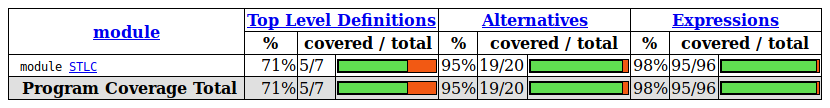
\includegraphics[width=0.85\linewidth]{Images/coverage_stlc}
\caption{Test coverage results for STLC.}
\vspace{-1ex}
\label{fig:coverage-stlc}
\end{figure}

As the interpreter of STLC is encoded in a unique module, we have just one line showing the coverage results for ``Top level definitions'' (71\%), ``Alternatives'' (95\%), and ``Expressions'' (98\%). Then, we used the detailed coverage description to see which part of code was not reached by the performed tests. Figure~\ref{fig:ty-stlc} shows a result of HPC with highlighted code (using the yellow color) for unreachable code.

\begin{figure}[!htb]
\centering
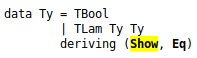
\includegraphics[width=0.3\linewidth]{Images/ty_stlc}
\caption{Unreachable code on STLC definition of types.}
\vspace{-1ex}
\label{fig:ty-stlc}
\end{figure}

This result is obviously correct, since we are not concerned in showing any information to the user (i.e., there is no instance to \ensuremath{\V{Show}})  when running our tests of properties. Figure~\ref{fig:step-stlc} shows a piece of code highlighted using the green color, which means that whenever the interpreter reaches the highlighted code, the result is always \ensuremath{\Con{True}}. Here again, the result is obvious, because the \ensuremath{\HK{otherwise}} keyword will always produce such result. 

\begin{figure}[!htb]
\centering
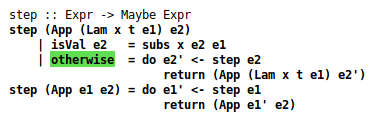
\includegraphics[width=0.57\linewidth]{Images/step_stlc}
\caption{Unreachable code on STLC evaluation.}
\label{fig:step-stlc}
\end{figure}

The last result we show for STLC is related to its type-checker. Figure~\ref{fig:typeof-stlc} shows the complete implementation of function \ensuremath{\HFun{typeof}} which encodes the static semantics of this calculus. By observing this results, we have two distinct parts highlighted with different colors. The first part appears in green, stating that the test \ensuremath{\V{t1}\;\D{\equiv}\;\V{t1'}} is always true, and as result the line in yellow is never reached. Indeed, this is the expected result for this code, since we are generating only well-typed expressions, which means that we should never return an error during type-checking. 

\begin{figure}[!htb]
\centering
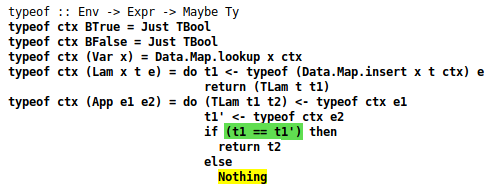
\includegraphics[width=0.75\linewidth]{Images/typeof_stlc}
\caption{Unreachable code on STLC type-checker.}
\label{fig:typeof-stlc}
\end{figure}

The presented statistics provided by HPC are very useful to improve the quality of tests, since we have information about each individual line of code performed when running the test suite. Specifically for the presented interpreter, we can say that although not covering all the source-code, we have good test cases, because code not reached by the interpreter would only be reached by ill-typed programs, i.e., error handling code.

\section{Featherweight Java}
\label{sec:pbt-fj}

To generate random programs in the context of FJ, we follow two distinct phases, expression and class generation, generalizing the approach presented in the last section, considering that FJ has a nominal type system instead of a structural one. Similarly to STLC, we specified a generation rule for each typing rule, both for expression generation and class table generation. This section summarizes the results of the papers ``Generating Random Well-Typed Featherweight Java Programs Using QuickCheck''~\cite{feitosa2018-2}, and ``A Type-Directed Algorithm to Generate Well-Typed Featherweight Java Programs''~\cite{feitosa2018-4}.

\subsection{Expression Generation}

We assume that a class table CT is a finite mapping between names and its corresponding classes. We let \emph{dom}(CT) denote the set of names in the domain of the finite mapping CT. An empty sequence is denoted by $\bullet$, and the length of a sequence \texttt{\={x}} is written \texttt{\#\={x}}. The generation algorithm also uses the function $\xi : [a] -> a$, which returns a random element from an input list. Similarly the previous section, we use set operations on lists (sequences) and its meaning is as usual.

The expression generation is represented by the following judgment:

\[
\textrm{CT ; $\Gamma$ ; C $\Rightarrow_e$ e}
\]

There CT is a class table, $\Gamma$ is a typing environment, C is a type name and e is the produced expression.

For generating \emph{variables}, we just need to select a name from the typing environment, which has a type C.

\[
\inference{}
          {\textrm{CT ; $\Gamma$ ; C $\Rightarrow_e \xi$ (\{ x $\mid$ $\Gamma$(x) = C \})}}[\footnotesize{[G-Var]}]
\]

For \emph{fields access}, we first need to generate a list of candidate type names for generating an expression with type C$'$ which has at least one field whose type is C. We name such list $\overline{C_c}$:

\[
\textrm{$\overline{C_c}$ = \{ C$_1$ $\mid$ C$_1$ $\in$ \emph{dom}(CT) $\land$ $\exists$ x. C x $\in$ \emph{fields}(C$_1$) \}}
\]

Now, we can build a random expression by using a type randomly chosen from it.

\[
\stackanchor{\textrm{C$'$ = $\xi$($\overline{C_c}$)}}
            {\textrm{CT ; $\Gamma$ ; C$'$ $\Rightarrow_e$ e}}
\]

Since type C$'$ can have more than one field with type C, we need to choose one of them (note that, by construction, such set is not empty).

\[
\textrm{C f = $\xi$(\{C x $\mid$ C x $\in$ \emph{fields}(C$'$)\}}
\]

The rule {\footnotesize G-Field} combines these previous steps to generate a field access expression:

\[
\inference{\textrm{$\overline{C_c}$ = \{C$_1$ $\mid$ C$_1$ $\in$ \emph{dom}(CT) $\land$ $\exists$ x. C x $\in$ \emph{fields}(C$_1$)\}} \\
           \textrm{C$'$ = $\xi$($\overline{C_c}$)} \\
           \textrm{CT ; $\Gamma$ ; C$'$ $\Rightarrow_e$ e} \\
           \textrm{C f = $\xi$(\{C x $\mid$ C x $\in$ \emph{fields}(C$'$)\}}}
          {\textrm{CT ; $\Gamma$ ; C $\Rightarrow_e$ e.f}}[\footnotesize{[G-Field]}]
\]
        
For \emph{method invocations}, we first need to find all classes which have method signatures with return type C. As before, we name such candidate class list as~$\overline{C_c}$.

\[
\textrm{$\overline{C_c}$ = \{C$_1$ $\mid$ C$_1$ $\in$ \emph{dom}(CT) $\land$ $\exists$ m \={D}. \emph{mtype}(m, C$_1$) = \={D} $->$ C\}}
\]

Next, we need to generate an expression e$_0$ from a type chosen from $\overline{C_c}$, we name such type as C$'$.

\[
\stackanchor{\textrm{C$'$ = $\xi$($\overline{C_c}$)}}
            {\textrm{CT ; $\Gamma$ ; C$'$ $\Rightarrow_e$ e$_0$}}
\]

From such type C$'$, we need to chose which method with return type C will be called. For this, we select a random signature from its list of candidate methods. 

\[
\stackanchor{\textrm{$\overline{M_c}$ = \{(m, \={D} $->$ C) $\mid$ $\exists$ m. \emph{mtype}(m , C$'$) = \={D} $->$ C\}}}
            {\textrm{(m$'$, \={D}$'$ $->$ C) = $\xi$($\overline{M_c}$)}}
\]

Next, we need to generate arguments for all formal parameters of method m$'$. For this, since arguments could be of any subtype of the formal parameter type, we need to choose it from the set of all candidate subtypes.

First, we define a function called subtypes, which return a list of all subtypes
of some type.

\[
\stackanchor{\textrm{\emph{subtypes}(CT, Object) = \{Object\}} \hspace{188pt}}
            {\textrm{\emph{subtypes}(CT, C) = \{C\} $\cup$ \emph{subtypes}(CT, D), if class C extends D $\in$ CT}}
\]

Using this function, we can build the list of arguments for a method call.

\[
\textrm{\={a} = \{e $\mid$ D $\in$ \={D}$'$ $\land$ CT ; $\Gamma$ ; $\xi$(subtypes(CT, D)) $\Rightarrow_e$ e \}}
\]

The rule {\footnotesize G-Invk} combines all these previous steps to produce a method call.
    
\[
\inference{\textrm{$\overline{C_c}$ = \{C$_1$ $\mid$ C$_1$ $\in$ \emph{dom}(CT) $\land$ $\exists$ m \={D}. \emph{mtype}(m, C$_1$) = \={D} $->$ C\}} \\
           \textrm{C$'$ = $\xi$($\overline{C_c}$)} \\
           \textrm{CT ; $\Gamma$ ; C$'$ $\Rightarrow_e$ e$_0$} \\
           \textrm{$\overline{M_c}$ = \{(m, \={D} $->$ C) $\mid$ $\exists$ m. \emph{mtype}(m , C$'$) = \={D} $->$ C\}} \\
           \textrm{(m$'$, \={D}$'$ $->$ C) = $\xi$($\overline{M_c}$)} \\
           \textrm{\={a} = \{e $\mid$ D $\in$ \={D}$'$ $\land$ CT ; $\Gamma$ ; $\xi$(subtypes(CT, D)) $\Rightarrow_e$ e\}}}
          {\textrm{CT ; $\Gamma$ ; C $\Rightarrow_e$ e$_0$.m$'$(\={a})}}[\footnotesize{[G-Invk]}]
\]

The generation of a random \emph{object creation} expression is straightforward: First, we need to get all field types of the class C and produce arguments for C's constructor parameters, as demonstrated by rule {\footnotesize G-New}.

\[
\inference{\textrm{\={F} = \{C$'$ $\mid$ C$'$ f $\in$ \emph{fields}(C)\}} \\
           \textrm{\={a} = \{e $\mid$ F $\in$ \={F} $\land$ CT ; $\Gamma$ ; $\xi$(\emph{subtypes}(CT, F)) $\Rightarrow_e$ e\}}}
          {\textrm{CT ; $\Gamma$ ; C $\Rightarrow_e$ new C(\={a})}}[\footnotesize{[G-New]}]
\]

We construct \emph{upper casts} expressions for a type C using
the {\footnotesize G-UCast} rule.

\[
\inference{\textrm{\={D} = \emph{subtypes}(CT, C)} \\
           %\textrm{C$'$ = $\xi$(\={D})} \\
           \textrm{CT ; $\Gamma$ ; $\xi$(\={D}) $\Rightarrow_e$ e}}
          {\textrm{CT ; $\Gamma$ ; C $\Rightarrow_e$ (C) e}}[\footnotesize{[G-UCast]}]
\]

Although we do not start a program with \emph{downcasts} or \emph{stupid casts}, because expressions generated by these typing rules can reduce to \emph{cast unsafe} terms~\cite{Igarashi:2001:FJM:503502.503505}, we defined the generation process in the rules {\footnotesize G-DCast} and {\footnotesize G-SCast}, since they can be used to build inner sub-expressions.

For generating downcasts, first we need the following function, which returns the set of super types of a given class name C.

\[
\stackanchor{\textrm{\emph{supertypes}(CT, Object) = $\bullet$} \hspace{235pt}}
            {\textrm{\emph{supertypes}(CT, C) = \{D\} $\cup$ \emph{supertypes}(CT, D), if class C extends D $\in$ CT}}
\]

Then, we can produce the rule {\footnotesize G-DCast} to generate a downcast expression.

\[
\inference{\textrm{\={D} = \emph{supertypes}(CT,C)} \\
           \textrm{CT ; $\Gamma$ ; $\xi$(\={D}) $\Rightarrow_e$ e}}
          {\textrm{CT ; $\Gamma$ ; C $\Rightarrow_e$ (C) e}}[\footnotesize{[G-DCast]}]
\]

The generation of stupid casts has a similar process, except that it generates a list of unrelated classes, as we can see in the first line of the rule {\footnotesize G-SCast}.

\[
\inference{\textrm{\={C} = \emph{dom}(CT) - (\emph{subtypes}(CT,C) $\cup$ \emph{supertypes}(CT,C))} \\
           \textrm{CT ; $\Gamma$ ; $\xi$(\={C}) $\Rightarrow_e$ e}}
          {\textrm{CT ; $\Gamma$ ; C $\Rightarrow_e $ (C) e}}[\footnotesize{[G-SCast]}]
\]

Considering the presented generation rules, we are able to produce well-typed expressions for each FJ's definitions.

\subsection{Class Table Generation}

To generate a class table, we assume the existence of an enumerable set $\overline{C_n}$ of class names and $\overline{V_n}$ of variable names. We let $\varphi : L -> C$ denote a function that returns a class name C from a given class declaration $L$. The inclusion of an item $x$ in a sequence $\overline{X}$ is denoted by $x : \overline{X}$, following Haskell's notation for lists. The generation rules are parameterized by an integer $n$ which determines the number of classes that will populate the resulting table, a limit $m$ for the number of members (attributes or methods) in each class and a limit $p$ for the number of formal parameters in the generated methods. This procedure is expressed by the following judgment:

\[
\textrm{CT ; n ; m ; p $\Rightarrow_{ct}$ CT$'$}
\]

It is responsible to generate $n$ classes using as input the information in class table CT (which can be empty), each class will have up to $m$ members. As a result, the judgment will produce a new class table CT$'$. As expected, this judgment is defined by recursion on $n$:

\[
\inference{}
          {\textrm{CT ; 0 ; m ; p $\Rightarrow_{ct}$ CT}}[\footnotesize{[CT-Base]}]
\]


\[
\inference{\textrm{CT ; m ; p $\Rightarrow_c$ L} \\
           \textrm{$\varphi$(L) L : CT ; n ; m ; p $\Rightarrow_{ct}$ CT$'$}}
          {\textrm{CT ; n + 1 ; m ; p $\Rightarrow_{ct}$ CT$'$}}[\footnotesize{[CT-Step]}]
\]         

Rule {\footnotesize CT-Base} specifies when the class table generation procedure stops. Rule {\footnotesize CT-Step} uses a specific judgment to generate a new class, inserts it in the class table CT, and generate the next $n$ classes using the recursive call $\varphi$(L) L : CT; n ; m ; p $\Rightarrow_{ct}$ CT$'$. The following judgment presents how classes are generated:

\[
\textrm{CT ; m ; p $\Rightarrow_c$ L}
\]

It generates a new class, with at most $m$ members, with at most $p$ formal parameters in each method, using as a starting point a given class table. First, we create a new name which is not in the domain of the input class table, using:

\[
\textrm{C = $\xi$($\overline{C_n}$ - (\emph{dom}(CT) $\cup$ \{Object\}))}
\]

This rule selects a random class name from the set $\overline{C_n}$ excluding the names in the domain of CT and Object. Next, we need to generate a valid super class name, which can be any of the set formed by the domain of current class table CT and Object:

\[
\textrm{D = $\xi$(\emph{dom}(CT) $\cup$ \{Object\})}
\]


After generating a class name and its super class, we need to generate its members. For this, we generate random values for the number of fields and methods, named fn and mn, respectively. Using such parameters we build the fields and methods for a given class. 

Field generation is straightforward. It proceeds by recursion on $n$, as shown below. Note that we maintain a set of already used attribute names $\overline{U_n}$ to avoid duplicates. 

\[
\inference{}
          {\textrm{CT ; 0 ; $\overline{U_n}$ $\Rightarrow_{fs}$ $\bullet$}}[\footnotesize{[G-Fields-Base]}] 
\]

\[
\inference{\textrm{C = $\xi$(\emph{dom}(CT) $\cup$ \{Object\})} \\
           \textrm{f = $\xi$($\overline{V_n}$ - $\overline{U_n}$)} \\
           \textrm{CT ; n ; f : $\overline{U_n}$ $\Rightarrow_{fs}$ \={C} \={f}}}
          {\textrm{CT ; n + 1 ; $\overline{U_n}$ $\Rightarrow_{fs}$ C f : \={C} \={f}}}[\footnotesize{[G-Fields-Step]}]
\]

Generation of the method list proceeds by recursion on $m$, as shown below. We also maintain a set of already used method names $\overline{U_n}$ to avoid method overload, which is not supported by FJ. The rule {\footnotesize G-Method-Step} uses a specific judgment to generate each method, which is described by rule {\footnotesize G-Method}.

\[
\inference{}
          {\textrm{CT ; C ; 0 ; p ; $\overline{U_n}$ $\Rightarrow_{ms}$ $\bullet$}}[\footnotesize{[G-Methods-Base]}]
\]

\[
\inference{\textrm{x = $\xi$($\overline{V_n}$ - $\overline{U_n}$)} \\
           \textrm{CT ; C ; p ; x $\Rightarrow_m$ M} \\
           \textrm{CT ; C ; m ; p ; x : $\overline{U_n}$ $\Rightarrow_{ms}$ \={M}}}
          {\textrm{CT ; C ; m + 1 ; p ; $\overline{U_n}$ $\Rightarrow_{ms}$ M : \={M}}}[\footnotesize{[G-Methods-Step]}]
\]

The rule {\footnotesize G-Method} uses an auxiliary judgment for generating formal parameters (note that we can generate an empty parameter list). To produce the expression, which defines the method body, we build a typing environment using the formal parameters and a variable \texttt{this} to denote this special object. Also, such expression is generated using a type that can be any of the possible subtypes of the method return type C$_0$.

\[
\inference{\textrm{n = $\xi$([$0..$(p - 1)])} \\
           \textrm{CT ; n ; $\bullet$ $\Rightarrow_{ps}$ \={C} \={x}} \\
           \textrm{C$_0$ = $\xi$(\emph{dom}(CT) $\cup$ \{Object\})} \\
           \textrm{$\Gamma$ = {\={C} \={x}, this : C}} \\
           \textrm{\={D} = \emph{subtypes}(CT,C$_0$)} \\
           \textrm{E$_0$ = $\xi$(\={D})} \\
           \textrm{CT ; $\Gamma$ ; E$_0$ $\Rightarrow_e$ e}}
          {\textrm{CT ; C ; p ; m $\Rightarrow_m$ (C$_0$ m (\={C} \={x}) \{return e;\})}}[\footnotesize{[G-Method]}]
\]

We create the formal parameters for methods using a simple recursive judgment that keeps a set of already used variable names $\overline{U_n}$ to ensure that all produced variables are distinct.

\[
\inference{}
          {\textrm{CT ; 0 ; $\overline{U_n}$ $\Rightarrow_{ps}$ $\bullet$}}[\footnotesize{[G-Param-Base]}]
\]

\[
\inference{\textrm{C = $\xi$(\emph{dom}(CT) $\cup$ \{Object\})} \\
           \textrm{x = $\xi$($\overline{V_n}$ - $\overline{U_n}$)} \\
           \textrm{CT ; n ; x : $\overline{U_n}$ $\Rightarrow_{ps}$ \={C} \={x}}}
          {\textrm{CT ; n + 1 ; $\overline{U_n}$ $\Rightarrow_{ps}$ (C x : \={C} \={x})}}[\footnotesize{[G-Param-Step]}]
\]

Finally, with the generated class name and its super class, we build the constructor definition using the judgment:

\[
\textrm{\emph{CT} ; C ; D $\Rightarrow_k$ K}
\]

Rule {\footnotesize G-Constr} represents the process to generate the constructor.

\[
\inference{\textrm{\={D} \={g} = \emph{fields}(D)} \\
           \textrm{\={C} \={f} = \emph{fields}(C) - \={D} \={g}}}
          {\textrm{CT ; C ; D $\Rightarrow_k$ ( C (\={D} \={g}, \={C} \={f}) \{ super(\={g}) ; this.\={f} = \={f} \} )}}[\footnotesize{[G-Constr]}]
\]

\pagebreak

The process for generating a complete class is summarized by rule {\footnotesize G-Class}, which is composed by all previously presented rules.

\[
\inference{\textrm{C = $\xi$($\overline{C_n}$ - (\emph{dom}(CT) $\cup$ \{Object\}))} \\
           \textrm{D = $\xi$(\emph{dom}(CT) $\cup$ \{Object\})} \\
           \textrm{fn = $\xi$([$1 .. $m])} \\
           \textrm{mn = $\xi$([$1 .. $(m - fn)])} \\
           \textrm{CT$'$ = C (class C extends D \{\}) : CT} \\
           \textrm{CT$'$ ; fn ; $\bullet$ $\Rightarrow_{fs}$ \={C} \={f}} \\
           \textrm{CT$''$ = C (class C extends D \{\={C} \={f}\}) : CT} \\
           \textrm{CT$''$ ; C ; mn ; p ; $\bullet$ $\Rightarrow_{ms}$ \={M}} \\
           \textrm{CT$'$ ; C ; D $\Rightarrow_k$ K}}
          {\textrm{CT ; m ; p $\Rightarrow_c$ (class C extends D \{ \={C} \={f}; K \={M} \})}}[\footnotesize{[G-Class]}]
\]

\vspace{8pt}

Considering the presented generation rules, we are able to fill a class table with well-formed classes in respect to FJ typing rules.

\subsection{Soundness of Program Generation}

The generation algorithm described in the previous section produces only well-typed FJ programs.

\begin{lemma}[Soundness of expression generation]
\label{lem:fj-seg}
Let \emph{CT} be a well-formed class table. For all $\Gamma$ and C $\in$ dom\emph{(CT)}, if \emph{CT} ; $\Gamma$ ; C $\Rightarrow_e$ e then exists D, such that $\Gamma \vdash$  e : D and D $<$: C.
\end{lemma}

\begin{proof}
The proof proceeds by induction on the derivation of \emph{CT} ; $\Gamma$ ; C $\Rightarrow_e$ e doing a case analysis on the last rule used to deduce \emph{CT} ; $\Gamma$ ; C $\Rightarrow_e$ e. We show some cases of the proof.

\vspace{5pt}

Case (G-Var): Then, e = x, for some variable x. By rule {\footnotesize G-Var}, x = $\xi$(\{y $\mid$ $\Gamma$(y) = C\}) and from this we can deduce that $\Gamma$(x) = C and the conclusion follows by rule {\footnotesize T-Var}.

\vspace{5pt}

Case (G-Invk): Then, e = e$_0$.m(\={e}) for some e$_0$ and \={e}; \emph{CT} ; $\Gamma$ ; C$'$ $\Rightarrow_e$ e$_0$, for some C$'$; there exists (m, \={D}$'$ $->$ C), such that \emph{mtype}(m, C$'$) = \={D} $->$ C and for all e$'$ $\in$ \={e}, D $\in$ \={D}$'$, \emph{CT} ; $\Gamma$ ; $\xi$(\emph{subtypes}(\emph{CT},D)) $\Rightarrow_e$ e$'$. By the induction hypothesis, we have that: $\Gamma$ $\vdash$ e$_0$ : D$'$, D$'$ $<$: C$'$, for all e$'$ $\in$ \={e}, D $\in$ \={D}$'$. $\Gamma$ $\vdash$ e$'$ : B, B $<$: D and the conclusion follows by the rule {\footnotesize T-Invk} and the definition of subtyping relation.
\end{proof}

\begin{lemma}[Soundness of subtypes]
\label{lem:fj-sos}
Let \emph{CT} be a well-formed class table and C $\in$ dom\emph{(CT)}.
For all D. if D $\in$ subtypes\emph{(CT},C\emph{)} then C $<$: D.
\end{lemma}

\begin{proof}
Straightforward induction on the structure of the result of \emph{subtypes}(CT, C).
\end{proof}

\begin{lemma}[Soundness of method generation]
\label{lem:fj-smg}
Let \emph{CT} be a well-formed class table and C $\in$ dom\emph{(CT)} $\cup$ \emph{\{Object\}}.
For all p and m, if \emph{CT} ; C ; p ; m $\Rightarrow_m$ \emph{C$_0$ m (\={C} \={x}) \{ \textnormal{return} e; \}} then \emph{C$_0$ m (\={C} \={x}) \{ \textnormal{return} e; \}} OK in C.
\end{lemma}

\begin{proof}
By rule {\footnotesize G-Method}, we have that:
\begin{itemize}
\item \={C} $\subseteq$ \emph{dom}(CT)
\item $\Gamma$ = \{\={C} \={x}, \texttt{this} : C\}
\item C$_0$ = $\xi$(\emph{dom}(CT) $\cup$ \{Object\})
\item \={D} = \emph{subtypes}(CT,C$_0$)
\item \emph{CT} ; $\Gamma$ ; E$_0$ $\Rightarrow_e$ e
\item E$_0$ = $\xi$(\={D})
\end{itemize}

By Lemma \ref{lem:fj-sos}, we have that for all D $\in$ \={D}, C$_0$ $<$: D.

By Lemma \ref{lem:fj-seg}, we have that $\Gamma$ $\vdash$ e : E$'$ and E$'$ $<$: E$_0$.

Since \emph{CT} is well-formed, then \emph{mtype}(m, C) = \={C} $->$ C$_0$ and the conclusion follows by rule \emph{method typing} and the definition of the subtyping relation.
\end{proof}

\begin{lemma}[Soundness of class generation]
\label{lem:fj-scg}
Let \emph{CT} be a well-formed class table. For all m, p, if \emph{CT} ; m ; p $\Rightarrow_c$ CD then CD OK.
\end{lemma}

\begin{proof}
By rule {\footnotesize G-Class}, we have that:

\begin{itemize}
\item CD = class C extends D \{ \={C} \={f} ; K \={M} \}
\item C = $\xi$($\overline{C_n}$ - (\emph{dom}(CT) $\cup$ Object))
\item D = $\xi$(\emph{dom}(CT) $\cup$ Object)
\item fn = $\xi$([$1..$m])
\item mn = $\xi$([$1..$(m - fn)])
\item \emph{CT}$'$ = C (class C extends D \{\}) : \emph{CT} 
\item \emph{CT}$'$ ; fn $\Rightarrow_{fs}$ \={C} \={f}
\item \emph{CT}$''$ = C (class C extends D \{ \={C} \={f}; \}) : \emph{CT}
\item \emph{CT}$''$ ; C ; mn ; p ; $\bullet$ $\Rightarrow_{ms}$ \={M}
\item \emph{CT}$'$ ; C ; D $\Rightarrow_k$ K
\end{itemize}

By Lemma \ref{lem:fj-smg}, we have that for all m. m $\in$ \={M}, m OK.

By rule {\footnotesize G-Constr} we have that K =  C (\={D} \={g}, \={C} \={f}) \{super(\={g}); this.\={f} = \={f};\}, where \={D} \={g} = fields(D).

The conclusion follows by rule \emph{class typing}.
\end{proof}

\begin{lemma}
\label{lem:fj-ctst}
Let \emph{CT} be a well-formed class table. For all n, m and p, if \emph{CT} ; n ; m ; p $\Rightarrow_{ct}$ \emph{CT}$'$ then for all C, D $\in$ dom\emph{(CT$'$)}, if C $<$: D and D $<$: C  then \emph{CT(C)} = \emph{CT(D)}.
\end{lemma}

\begin{proof}
By induction on n.

\vspace{5pt}

Case n = 0: We have that CT$'$ = CT. Conclusion follows by the fact that CT is a well-formed class table.

\vspace{5pt}

Case n = n$'$ + 1: Suppose C, D $\in$ \emph{dom}(CT$'$), C $<$: D and D $<$: C. By the induction hypothesis we have that for all CT$_1$, C$'$, D$'$ $\in$ CT$_1$, if C$'$ $<$: D$'$ and D$'$ $<$: C$'$ then C$'$ = D$'$, where CT ; n ; m ; p $\Rightarrow_{ct}$ CT$_1$. Let L be
a class such that CT ; m ; p $\Rightarrow_c$ L. By Lemma \ref{lem:fj-scg}, we have L OK in CT. By
the induction hypothesis on $\varphi$(L) L : CT ; n ; m ; p $\Rightarrow_{ct}$ CT$'$ and
rule {\footnotesize CT-Step} we have the desired conclusion.
\end{proof}

\begin{lemma}[Soundness of class table generation]
\label{lem:fj-sctg}
Let \emph{CT} be a well-formed class table. For all n, m and p, if \emph{CT} ; n ; m ; p $\Rightarrow_{ct}$ \emph{CT}$'$ then \emph{CT}$'$ is a well-formed class table.
\end{lemma}

\begin{proof}
  By induction on n.

\vspace{5pt}

  Case n = 0: We have that CT$'$ = CT and the conclusion follows.

\vspace{5pt}

  Case n = n$'$ + 1: By rule {\footnotesize CT-Step} we have that:

\begin{itemize}
\item CT ; m ; p $\Rightarrow_c$ L
\item $\varphi$(L) L : CT ; n ; m ; p $\Rightarrow_{ct}$ CT$'$
\end{itemize}

By Lemma \ref{lem:fj-scg}, we have that L \emph{OK}. By the induction hypothesis we have that CT$'$ is a well-formed class table. By Lemma \ref{lem:fj-ctst}, we have that subtyping in CT$'$ is antisymmetric. Conclusion follows by the definition of a well-formed class table.
\end{proof}

\begin{theorem}[Soundness of program generation]
For all n, m and p, if $\bullet$ ; n ; m ; p $\Rightarrow_{ct}$ \emph{CT} then:

\begin{enumerate}
\item \emph{CT} is a well-formed class table.
\item For all \emph{C} $\in$ \emph{CT}, we have \emph{C} OK.
\end{enumerate}
\end{theorem}

\begin{proof}
Corollary of Lemmas \ref{lem:fj-scg}, \ref{lem:fj-ctst} and \ref{lem:fj-sctg}.
\end{proof}

\subsection{QuickChecking Semantic Properties}

As a proof of concept we have implemented an interpreter following the semantics of FJ, and we used random generated programs to check this interpreter against some properties, including those for type-soundness. The properties were specified and tested using QuickCheck~\cite{Claessen:2000:QLT:351240.351266}. 

Considering that testing requires additional programming, there is a natural risk that the testing code itself contain bugs~\cite{Midtgaard:2017:EQC:3136534.3110259}. In order to reduce the risk of bugs in our implementation, we have tested it with QuickCheck, by using our interpreter and the test generators. We checked the following:

\begin{itemize}
\item That our custom generator produces only well-formed class tables.
\vspace{-1ex}
\item That our custom generator produces only well-typed expressions, according to a randomly generated class table.
\vspace{-1ex}
\item And if all generated expressions are cast-safe.
\end{itemize}

We started defining a function to check if generated class tables are well-formed, as follows:

\begin{hscode}\SaveRestoreHook
\column{B}{@{}>{\hspre}l<{\hspost}@{}}%
\column{3}{@{}>{\hspre}l<{\hspost}@{}}%
\column{5}{@{}>{\hspre}l<{\hspost}@{}}%
\column{14}{@{}>{\hspre}l<{\hspost}@{}}%
\column{E}{@{}>{\hspre}l<{\hspost}@{}}%
\>[B]{}\HFun{prop\_genwellformedct}\;\Con{::}\;\HT{Bool}{}\<[E]%
\\
\>[B]{}\HFun{prop\_genwellformedct}\;\mathrel{=}\;{}\<[E]%
\\
\>[B]{}\hsindent{3}{}\<[3]%
\>[3]{}\HK{forAll}\;(\HFun{genClassTable})\;\HN{\$}\;{}\<[E]%
\\
\>[3]{}\hsindent{2}{}\<[5]%
\>[5]{}\lambda \;\V{ct}\;\to \;\HFun{Data.List.all}\;{}\<[E]%
\\
\>[5]{}\hsindent{9}{}\<[14]%
\>[14]{}(\lambda \;(\V{c,cl})\;\to \;\HFun{classTyping}\;\V{cl}\;\HC{Data.Map.empty}\;\V{ct})\;(\HFun{Data.Map.toList}\;\V{ct}){}\<[E]%
\ColumnHook
\end{hscode}\resethooks

The above code uses the QuickCheck function \ensuremath{\HK{forAll}}, which mimics the universal quantifier $\forall$, generating a user-defined number of instances of class tables, and testing if all produced classes and interfaces inside a given class table are well-formed, by running the function \ensuremath{\HFun{classTyping}}.

We also defined a function to test if the generated expressions are well-typed, as in the following piece of code. This function starts by generating an instance of a class table \ensuremath{\V{ct}}. After that, it randomly chooses a type \ensuremath{\V{t}} present in the class table (class or interface). Then, it uses the produced \ensuremath{\V{ct}} and an empty environment, to generate an expression of type \ensuremath{\V{t}}. In the end, by using the function \ensuremath{\HFun{typeof}}, it checks if the expression has indeed the type \ensuremath{\V{t}}.

\begin{hscode}\SaveRestoreHook
\column{B}{@{}>{\hspre}l<{\hspost}@{}}%
\column{3}{@{}>{\hspre}l<{\hspost}@{}}%
\column{5}{@{}>{\hspre}l<{\hspost}@{}}%
\column{18}{@{}>{\hspre}l<{\hspost}@{}}%
\column{E}{@{}>{\hspre}l<{\hspost}@{}}%
\>[B]{}\HFun{prop\_genwelltypedexpr}\;\Con{::}\;\HT{Bool}{}\<[E]%
\\
\>[B]{}\HFun{prop\_genwelltypedexpr}\;\mathrel{=}\;{}\<[E]%
\\
\>[B]{}\hsindent{3}{}\<[3]%
\>[3]{}\HK{forAll}\;(\HFun{genClassTable})\;\HN{\$}\;{}\<[E]%
\\
\>[3]{}\hsindent{2}{}\<[5]%
\>[5]{}\lambda \;\V{ct}\;\to \;\HK{forAll}\;(\HFun{genType}\;\V{ct})\;\HN{\$}\;{}\<[E]%
\\
\>[3]{}\hsindent{2}{}\<[5]%
\>[5]{}\lambda \;\V{t}\;\to \;\HK{forAll}\;(\HFun{genExpression}\;\V{ct}\;\HC{Data.Map.empty}\;\V{t})\;\HN{\$}\;{}\<[E]%
\\
\>[3]{}\hsindent{2}{}\<[5]%
\>[5]{}\lambda \;\V{e}\;\to \;\HFun{either}\;(\HFun{const}\;\Con{False})\;{}\<[E]%
\\
\>[5]{}\hsindent{13}{}\<[18]%
\>[18]{}(\lambda \;(\HC{TypeClass}\;\V{t'})\;\to \;\V{t}\;\D{\equiv}\;\V{t'})\;{}\<[E]%
\\
\>[5]{}\hsindent{13}{}\<[18]%
\>[18]{}(\HFun{typeof}\;\HC{Data.Map.empty}\;\V{ct}\;\V{e}){}\<[E]%
\ColumnHook
\end{hscode}\resethooks

As a last check for our generators, the following function tests if a produced expression is \emph{cast-safe}, i.e., the subject expression is a subtype of the target type~\cite{Igarashi:2001:FJM:503502.503505}.

\begin{hscode}\SaveRestoreHook
\column{B}{@{}>{\hspre}l<{\hspost}@{}}%
\column{3}{@{}>{\hspre}l<{\hspost}@{}}%
\column{4}{@{}>{\hspre}l<{\hspost}@{}}%
\column{9}{@{}>{\hspre}l<{\hspost}@{}}%
\column{12}{@{}>{\hspre}l<{\hspost}@{}}%
\column{24}{@{}>{\hspre}l<{\hspost}@{}}%
\column{26}{@{}>{\hspre}l<{\hspost}@{}}%
\column{E}{@{}>{\hspre}l<{\hspost}@{}}%
\>[B]{}\HFun{prop\_gencastsafeexpr}\;\Con{::}\;\HT{Bool}{}\<[E]%
\\
\>[B]{}\HFun{prop\_gencastsafeexpr}\;\mathrel{=}\;{}\<[E]%
\\
\>[B]{}\hsindent{3}{}\<[3]%
\>[3]{}\HK{forAll}\;(\HFun{genClassTable})\;\HN{\$}\;{}\<[E]%
\\
\>[3]{}\hsindent{1}{}\<[4]%
\>[4]{}\lambda \;\V{ct}\;\to \;\HK{forAll}\;(\HFun{genType}\;\V{ct})\;\HN{\$}\;{}\<[E]%
\\
\>[3]{}\hsindent{1}{}\<[4]%
\>[4]{}\lambda \;\V{t}\;\to \;\HK{forAll}\;(\HFun{genExpression}\;\V{ct}\;\HC{Data.Map.empty}\;\V{t})\;\HN{\$}\;{}\<[E]%
\\
\>[3]{}\hsindent{1}{}\<[4]%
\>[4]{}\lambda \;\V{e}\;\to \;{}\<[12]%
\>[12]{}\HK{case}\;\V{e}\;\HK{of}\;{}\<[E]%
\\
\>[4]{}\hsindent{5}{}\<[9]%
\>[9]{}(\HC{Cast}\;\V{c}\;\V{e})\;\to \;{}\<[24]%
\>[24]{}\HK{case}\;(\HFun{typeof}\;\HC{Data.Map.empty}\;\V{ct}\;\V{e})\;\HK{of}\;{}\<[E]%
\\
\>[24]{}\hsindent{2}{}\<[26]%
\>[26]{}\HC{Right}\;(\HC{TypeClass}\;\V{t'})\;\to \;\HFun{subtyping}\;\V{t'}\;\V{c}\;\V{ct}\;{}\<[E]%
\\
\>[24]{}\hsindent{2}{}\<[26]%
\>[26]{}\anonymous \;\to \;\Con{False}\;{}\<[E]%
\\
\>[4]{}\hsindent{5}{}\<[9]%
\>[9]{}\anonymous \;\to \;\Con{True}{}\<[E]%
\ColumnHook
\end{hscode}\resethooks

Thanks to these checks we found and fixed a number of programming errors in our generator, and in our interpreter implementation. Although testing can't state correctness, we gain a high-degree of confidence in using the generated programs. 

We have used our test suite as a lightweight manner to check the properties of \emph{preservation} and \emph{progress} presented in the FJ paper. The informal (non-mechanized) proofs were also modeled as Haskell functions to be used with QuickCheck. 

The preservation (subject reduction) property is presented by Theorem 2.4.1 (p. 406 of \cite{Igarashi:2001:FJM:503502.503505}), stating that ``\emph{If $\Gamma \vdash$ \textnormal{e: T} and \textnormal{e} $->$ \textnormal{e}$'$, then $\Gamma \vdash$ \textnormal{e}$'$\textnormal{: T}$'$ \textnormal for some \textnormal{T}$'$ $<$\textnormal{:} \textnormal{T}}.''. Our function was modeled as follows:

\begin{hscode}\SaveRestoreHook
\column{B}{@{}>{\hspre}l<{\hspost}@{}}%
\column{3}{@{}>{\hspre}l<{\hspost}@{}}%
\column{11}{@{}>{\hspre}l<{\hspost}@{}}%
\column{14}{@{}>{\hspre}l<{\hspost}@{}}%
\column{E}{@{}>{\hspre}l<{\hspost}@{}}%
\>[B]{}\HFun{prop\_preservation}\;\Con{::}\;\HT{Bool}{}\<[E]%
\\
\>[B]{}\HFun{prop\_preservation}\;\mathrel{=}\;{}\<[E]%
\\
\>[B]{}\HK{forAll}\;(\HFun{genClassTable})\;\HN{\$}\;{}\<[E]%
\\
\>[B]{}\hsindent{3}{}\<[3]%
\>[3]{}\lambda \;\V{ct}\;\to \;\HK{forAll}\;(\HFun{genType}\;\V{ct})\;\HN{\$}\;{}\<[E]%
\\
\>[B]{}\hsindent{3}{}\<[3]%
\>[3]{}\lambda \;\V{t}\;\to \;\HK{forAll}\;(\HFun{genExpression}\;\V{ct}\;\HC{Data.Map.empty}\;\V{t})\;\HN{\$}\;{}\<[E]%
\\
\>[B]{}\hsindent{3}{}\<[3]%
\>[3]{}\lambda \;\V{e}\;\to \;\HFun{either}\;(\HFun{const}\;\Con{False})\;{}\<[E]%
\\
\>[3]{}\hsindent{8}{}\<[11]%
\>[11]{}(\lambda \;(\HC{TypeClass}\;\V{t'})\;\to \;\HFun{subtyping}\;\V{t'}\;\V{t}\;\V{ct})\;{}\<[E]%
\\
\>[3]{}\hsindent{8}{}\<[11]%
\>[11]{}(\HK{case}\;(\HFun{eval'}\;\V{ct}\;\V{e})\;\HK{of}\;{}\<[E]%
\\
\>[11]{}\hsindent{3}{}\<[14]%
\>[14]{}\HC{Just}\;\V{e'}\;\to \;\HFun{typeof}\;\HC{Data.Map.empty}\;\V{ct}\;\V{e'}\;{}\<[E]%
\\
\>[11]{}\hsindent{3}{}\<[14]%
\>[14]{}\anonymous \;\to \;\HFun{throwError}\;(\HC{UnknownError}\;\V{e})){}\<[E]%
\ColumnHook
\end{hscode}\resethooks

As we can see in the code, after generating an instance for \ensuremath{\V{ct}}, a type \ensuremath{\V{t}}, and an expression \ensuremath{\V{e}} of type \ensuremath{\V{t}}, a reduction step is performed by function \ensuremath{\HFun{eval'}} over expression \ensuremath{\V{e}} producing an \ensuremath{\V{e'}}. Then, the function \ensuremath{\HFun{typeof}} is used to obtain the type of \ensuremath{\V{e'}}. Last, the \ensuremath{\HFun{subtyping}} function is used to check if the expression keeps the typing relation after a reduction step.

Similarly, we modeled (as follows) a function for the progress property (Theorem 2.4.2, p. 407~\cite{Igarashi:2001:FJM:503502.503505}, which states that a well-typed expression does not get stuck.

\begin{hscode}\SaveRestoreHook
\column{B}{@{}>{\hspre}l<{\hspost}@{}}%
\column{3}{@{}>{\hspre}l<{\hspost}@{}}%
\column{5}{@{}>{\hspre}l<{\hspost}@{}}%
\column{E}{@{}>{\hspre}l<{\hspost}@{}}%
\>[B]{}\HFun{prop\_progress}\;\Con{::}\;\HT{Bool}{}\<[E]%
\\
\>[B]{}\HFun{prop\_progress}\;\mathrel{=}\;{}\<[E]%
\\
\>[B]{}\hsindent{3}{}\<[3]%
\>[3]{}\HK{forAll}\;(\HFun{genClassTable})\;\HN{\$}\;{}\<[E]%
\\
\>[3]{}\hsindent{2}{}\<[5]%
\>[5]{}\lambda \;\V{ct}\;\to \;\HK{forAll}\;(\HFun{genType}\;\V{ct})\;\HN{\$}\;{}\<[E]%
\\
\>[3]{}\hsindent{2}{}\<[5]%
\>[5]{}\lambda \;\V{t}\;\to \;\HK{forAll}\;(\HFun{genExpression}\;\V{ct}\;\HC{Data.Map.empty}\;\V{t})\;\HN{\$}\;{}\<[E]%
\\
\>[3]{}\hsindent{2}{}\<[5]%
\>[5]{}\lambda \;\V{e}\;\to \;\HFun{isValue}\;\V{ct}\;\V{e}\;\mathrel{\vee}\;\HFun{maybe}\;(\Con{False})\;(\HFun{const}\;\Con{True})\;(\HFun{eval'}\;\V{ct}\;\V{e}){}\<[E]%
\ColumnHook
\end{hscode}\resethooks
        
\vspace{-1ex}

This function also generates a class table, a type, and an expression of that type. Then it checks that or the expression is a value, or it can take a reduction step through the function \ensuremath{\HFun{eval'}}.

\subsection{Measuring the Quality of Tests}

We also ran many thousands of tests for the presented functions, all of them with success. Then, similarly to the previous section, we measured the quality of our tests with HPC by checking how much of the code base was covered by our test suite. Results of code coverage for each module (evaluator, type-checker, auxiliary functions, and total, respectively) are presented in Figure \ref{fig:coverage}.

\begin{figure}[!htb]
\centering
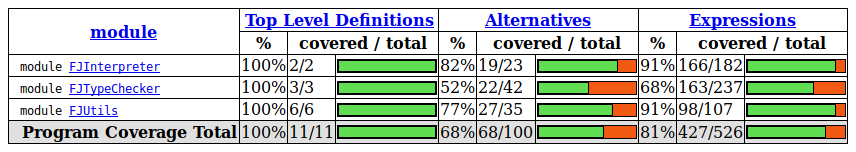
\includegraphics[width=0.95\linewidth]{Images/coverage_fjqc}
\caption{Test coverage results for FJ.}
\vspace{-1ex}
\label{fig:coverage}
\end{figure}

In Figure \ref{fig:fj-eval} we present a piece of code of our evaluator with unreachable code highlighted.

\begin{figure}[!htb]
\centering
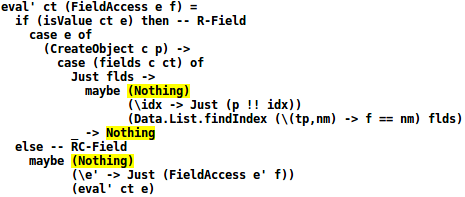
\includegraphics[width=0.70\linewidth]{Images/eval_fj}
\caption{Unreachable code on FJ evaluation.}
\label{fig:fj-eval}
\end{figure}

There we can note that to reach the highlighted code it is necessary: (1) the field \ensuremath{\V{f}} is not found in the fields of class \ensuremath{\V{c}}; (2) an error processing function \ensuremath{\HFun{eval'}} for the subexpression \ensuremath{\V{e}}. Both cases represent stuck states, which can be only executed if we have an ill-typed expression. As stated on type soundness proofs~\cite{Igarashi:2001:FJM:503502.503505}, a well-typed expression does not get stuck.

Similarly, Figure \ref{fig:typeof} shows a piece of code of our type-checker with unreachable code highlighted.

\begin{figure}[!htb]
\centering
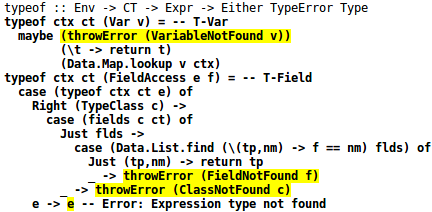
\includegraphics[width=0.68\linewidth]{Images/typeof_fj}
\caption{Unreachable code on FJ type-checker.}
\label{fig:typeof}
\end{figure}

We notice that the highlighted code would be executed only if: (1) we have an undefined variable in the typing context $\Gamma$; (2) the code is using a field that is not present in the class of current expression; (3) the type of sub-expression \ensuremath{\V{e}} could not be obtained. In all situations, we have an ill-typed program.

Finally, Figure~\ref{fig:fields} shows a piece of code of our auxiliary functions, where the highlighted code could be reached in two cases: (1) the class \ensuremath{\V{c}} is not present on the class table; (2) performing \ensuremath{\HFun{fields}} on a base class results in an error. This would only happen if we had an ill-typed program.

\begin{figure}[!htb]
\centering
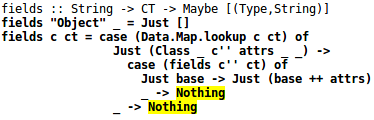
\includegraphics[width=0.57\linewidth]{Images/fields_fj}
\caption{Unreachable code on FJ auxiliary functions.}
\label{fig:fields}
\end{figure}

Although not having 100\% of code coverage, our test suite was capable to verify the main safety properties presented in FJ paper, by exercising on randomly generated programs of increasing size. By analyzing test coverage results, we could observe that code not reached by test cases consists of stuck states on program semantics or error control for expressions that are ill-typed. 

After testing our generation procedure against our hand-written interpreter, we compile the generated ASTs of FJ to regular Java code, and we created a QuickCheck property to export the generated code to a Java file, and to compile it using the `javac' compiler (the closest implementation of Java Specification Language), which was assumed as an oracle for our algorithm. The function \ensuremath{\HFun{prop\_compile}} (shown below) first generates a class table, a type, and an expression. Then it writes the code into a Java file (\ensuremath{\HS{\text{``}program.java\text{''}}}), and invokes the `javac' compiler passing this program as parameter, checking for success or failure in the process. In case of failure, QuickCheck presents the generated code as a counter example of the property.

\begin{hscode}\SaveRestoreHook
\column{B}{@{}>{\hspre}l<{\hspost}@{}}%
\column{4}{@{}>{\hspre}l<{\hspost}@{}}%
\column{6}{@{}>{\hspre}l<{\hspost}@{}}%
\column{9}{@{}>{\hspre}l<{\hspost}@{}}%
\column{E}{@{}>{\hspre}l<{\hspost}@{}}%
\>[B]{}\HFun{prop\_compile}\;\mathrel{=}\;{}\<[E]%
\\
\>[B]{}\HK{forAll}\;(\HFun{genClassTable})\;\HN{\$}\;{}\<[E]%
\\
\>[B]{}\hsindent{4}{}\<[4]%
\>[4]{}\lambda \;\V{ct}\;\to \;\HK{forAll}\;(\HFun{genType}\;\V{ct})\;\HN{\$}\;{}\<[E]%
\\
\>[B]{}\hsindent{4}{}\<[4]%
\>[4]{}\lambda \;\V{t}\;\to \;\HK{forAll}\;(\HFun{genExpression}\;\V{ct}\;\HC{Data.Map.empty}\;\V{t})\;\HN{\$}\;{}\<[E]%
\\
\>[B]{}\hsindent{4}{}\<[4]%
\>[4]{}\lambda \;\V{e}\;\to \;\HFun{monadicIO}\;\HN{\$}\;{}\<[E]%
\\
\>[4]{}\hsindent{2}{}\<[6]%
\>[6]{}\HK{do}\;\V{f}\;\leftarrow \;\HFun{run}\;(\HFun{writeFile}\;\HS{\text{``}program.java\text{''}}\;(\HFun{formatJavaProgram}\;\V{ct}\;\V{e}))\;{}\<[E]%
\\
\>[6]{}\hsindent{3}{}\<[9]%
\>[9]{}(\V{ex,out,err})\;\leftarrow \;\HFun{run}\;(\HFun{readProcessWithExitCode}\;\HS{\text{``}javac\text{''}}\;\V{[}\HS{\text{``}programa.java\text{''}}\V{]}\;\HS{\text{``}\text{''}})\;{}\<[E]%
\\
\>[6]{}\hsindent{3}{}\<[9]%
\>[9]{}\HFun{assert}\;(\V{ex}\;\D{\equiv}\;\HC{ExitSuccess}){}\<[E]%
\ColumnHook
\end{hscode}\resethooks

By using this function, while developing our code generator we were able to find two problems in our implementation when compiling it with `javac'. The first occurred when generating an expression with a \emph{cast}, where we notice lack of parenthesis on the cast expression, which caused an error of precedence. Another problem we found was the size limit for a method, since the Java Virtual Machine specification limits the size of generated Java byte code for each method in a class to the maximum of 64Kb. This limitation caused the JVM to throw \ensuremath{\HC{java.lang.VerifyError}} at runtime when the method size exceeded this limit. Both bugs were easily corrected by using the presented counter examples, and after that 100\% of the test cases were successfully performed.

\section{Semantics of Java 8 features in Featherweight Java}
\label{sec:fjlam}

In order to explore in depth the property-based testing approach regarding programming language properties, we extended Featherweight Java with new features. We defined the formal semantics of \emph{$\lambda$-expressions} and \emph{default methods} which were added in the kernel of Java in the release of Java Development Kit version 8 (JDK 8). By using $\lambda$-expressions a programmer can treat functions as a method argument, or code as data in Java in a similar way functional languages work, offering a programming model that fuses the object-oriented and functional paradigms. The text presented in this section is based upon our paper ``Property-based Testing the Semantics of Java 8 Features in Featherweight Java''~\cite{feitosa2018-3}. 

\pagebreak

\subsection{Extended Definitions}

The abstract syntax of FJ augmented with interfaces, $\lambda$-expressions and default methods is given in Figure \ref{fig:fje-syntax}, where $T$ represents type declarations, $L$ and $P$ express classes and interfaces, $K$ represents constructors (presented earlier), $S$ stands for signatures, $M$ for methods, and $e$ refers to the possible expressions. We use the meta-variables $C$, $D$, and $E$ to represent class names, $I$, and $J$ to represent interface names, and $T$, $U$, and $V$ to represent generic names for classes or interfaces. Other definitions are similar to those presented earlier in this chapter.

\begin{figure}[!htb]
\[
\begin{array}{llr}
  T ::= & \ \ \ \ \ \ \ \ \ \ \ \ \ \ \ \ \ \ \ \ \ \ \ \ \ \ \ \ \ \ \ \ \ \ \ \ \ \ & \textrm{type definitions} \\
        & C \mid I & \\
  L ::= & & \textrm{class declarations} \\
        & class ~ C ~ extends ~ C ~ implements ~ \overline{I} ~ \{ \overline{T} ~ \overline{f}; K ~ \overline{M} \} & \\
  P ::= & & \textrm{interface declarations} \\
        & interface ~ I ~ extends ~ \overline{I} ~ \{ \overline{S}; ~ default ~ \overline{M} \} & \\
  S ::= & & \textrm{signature declarations} \\
        & T ~ m(\overline{T} ~ \overline{x}) & \\
  M ::= & & \textrm{method declarations} \\
        & S ~ \{ ~ return ~ e; \} & \\
  e ::= & & \textrm{expressions: } \\
        & \cdots & \textrm{original FJ constructors} \\
        & (\overline{T} ~ \overline{x}) \rightarrow e & \lambda\textrm{-expression} \\
\end{array}
\]
\caption{Syntactic definitions for the extended FJ.}
\label{fig:fje-syntax}
\end{figure}

The differences from original FJ~\cite{Igarashi:2001:FJM:503502.503505} were given firstly by the introduction of \emph{interface declarations}, where $interface ~ I ~ extends ~ \overline{I} ~ \{ ~ \overline{S}; ~ default ~ \overline{M} ~ \}$ introduces an interface named $I$ with a list of super-interfaces $\overline{I}$. The new interface defines a list of signatures $\overline{S}$ and a list of default methods $default ~ \overline{M}$. For completeness, since Java's semantics allows a class to implement a list of interfaces, we changed the \emph{class declarations} accordingly. Second, the \emph{signature declarations} were added representing prototypes for abstract and concrete methods, where $T ~ m(\overline{T} ~ \overline{x})$ introduces a method named $m$, a return type $T$, and parameters $\overline{x}$ of types $\overline{T}$. As a consequence, the \emph{method declarations} were also modified. Lastly, we added the constructor for \emph{$\lambda$-expressions}, where $(\overline{T} ~ \overline{x}) -> e$ represents an anonymous function, which has a list of arguments with type $\overline{T}$ and names $\overline{x}$, and a body expressions $e$. 

The class table was also modified to accept both class and interface declarations. Therefore, a class table \emph{CT} is a mapping from class or interface names, to class or interface declarations, $L$ or $P$ respectively. It still should satisfy some conditions, such as each type $T$ should be in \emph{CT}, except $Object$, which is a special class; and there are no cycles in the sub-typing relation. Thereby, a program is a pair $(CT, e)$ of a class table and an expression. For brevity, we omit from this text the details about auxiliary definitions (\emph{fields}, \emph{mtype}, \emph{mbody}, \emph{$\lambda$mark} and \emph{abs-methods}), sub-typing, and the dynamic semantics, but these definitions can be found in~\cite{feitosa2018-3}. We explain the meaning of these definitions as they appear in the sequence of this text.

Since our generation procedure relies on the typing rules, we show in Figure~\ref{fig:fje-typing} the new typing rule {\footnotesize\textrm{T-Lam}}, which was added to type the $\lambda$-expression constructor. This rule first checks if $I$ is a functional interface\footnote{A functional interface is an interface that contains one and only one abstract method.}, using the function \emph{abs-methods} which should bring information about its only method signature. Next, we use our $\lambda$mark\footnote{A detailed explanation about this definition and its use can be found in our paper~\cite{feitosa2018-3}} definition to annotate the source-code with types for $\lambda$-expressions. Lastly, this rule verifies if the resulting type of the body is a sub-type of the return type of the method $m$.

\begin{figure}[!htb]
\[
\begin{array}{c} 
\inference{\textrm{abs-methods(I) = \{T m(\={T} \={y})\}} \\
          \textrm{$\lambda$mark(e,T) = e$'$ \ \ \ \ \={x}: \={T}, $\Gamma \vdash$ e$'$ : U \ \ \ \ \ U $<:$ T}}
          {\textrm{$\Gamma \vdash$ (I) ((\={T} \={x}) $->$ e) : I}}[[T-Lam]]
\end{array}
\]
\caption{Typing $\lambda$-expressions in FJ.}
\label{fig:fje-typing}
\end{figure}

We also had to add a rule to check if interfaces are well-formed, as shown in Figure \ref{fig:fje-ityping}. Roughly, this rule checks if all \emph{default methods} are well-formed (using the rule presented in the original FJ paper~\cite{Igarashi:2001:FJM:503502.503505}), and that there is at least one abstract method in such interface definition.

\begin{figure}[!htb]
\[
\begin{array}{c} 
\inference{\textrm{\={M} OK in I \ \ \ \ abs-methods(I) $\neq \bullet$}}
          {\textrm{interface I extends \={I} \{ \={S}; default \={M} \} OK}}
\vspace{5pt}
\end{array}
\]
\caption{Interface typing in FJ.}
\label{fig:fje-ityping}
\end{figure}

Having defined the new rules, we proved in~\cite{feitosa2018-3} the subject reduction and progress to demonstrate type soundness for the Java 8 features of $\lambda$-expressions and default methods analogously to FJ. We kept the theorem names of the original FJ paper~\cite{Igarashi:2001:FJM:503502.503505}, presenting only the new cases for each of them.

\begin{lemma}[Term substitution preserves typing]
\label{lem:fje-subs}
	\label{lem:subs}
	If $\Gamma, \overline{x} : \overline{U} \vdash e : U$ and $\Gamma \vdash \overline{d} : \overline{U_0}$ where $\overline{U_0} <: \overline{U}$, then $\Gamma \vdash [\overline{x} \mapsto \overline{d}]e : T$ for some $T <: U$.
\end{lemma}

\begin{proof}
  By induction on the derivation of $\Gamma, \overline{x} : \overline{U} \vdash e : U$ with case analysis on the typing rule used. It extends the original lemma for FJ (Lemma A.1.2~\cite{Igarashi:2001:FJM:503502.503505}) with the following case:
  
\vspace{5pt}
  
Case (T-Lam). $e = (I)((\overline{T} ~ \overline{x_0}) -> e_0)$, \emph{abs-methods}$(I)$ = $\{T_0 ~ m(\overline{T} ~ \overline{y})\}$, and $\Gamma, \overline{x} : \overline{U}, \overline{x_0} : \overline{T} \vdash e_0 : V$ where $V <: T_0$. By the induction hypothesis $\Gamma, \overline{x_0} : \overline{T} \vdash [\overline{x} \mapsto \overline{d}]e_0 : V$, finishing the case by applying the rule T-Lam.
\end{proof}

\begin{theorem}[Subject reduction]
	\label{th:preservation}
	If $\Gamma \vdash e : T$ and $e \rightarrow e'$, then $\Gamma \vdash e' : T'$ for some $T' <: T$.
\end{theorem}

\begin{proof}
By induction on the reduction $e \rightarrow e'$, with a case analysis on the reduction rule used. It extends the original proof~\cite{Igarashi:2001:FJM:503502.503505} of the corresponding theorem for FJ with the following cases:

\vspace{5pt}

Case (R-Default). $e = ((I)((\overline{T} ~ \overline{x}) -> e_0)).m(\overline{u})$, \emph{mbody}$(m, I) = (\overline{y}, e_1)$, and by rules {\footnotesize T-Invk} and {\footnotesize T-Lam}, we have: $\Gamma \vdash ((I)((\overline{T} ~ \overline{x}) -> e_0)): I$, \emph{mtype}$(m, I) = \overline{U} -> U$, $\Gamma \vdash \overline{u} : \overline{T}$, and $\overline{T} <: \overline{U}$. Furthermore, $e' = [\overline{u} \mapsto \overline{y}]e_1$ and by the Lemma \ref{lem:fje-subs}, $\Gamma \vdash e' = [\overline{u} \mapsto \overline{y}]e_1 : T$ for some $T <: U$.

Case (R-Lam). $e = ((I)((\overline{T} ~ \overline{x}) -> e_0)).m(\overline{u})$, and by rules {\footnotesize T-Invk} and {\footnotesize T-Lam}, we have: $\Gamma \vdash ((I)((\overline{T} ~ \overline{x}) -> e_0)): I$, \emph{mtype}$(m, I) = \overline{U} -> U$, $\Gamma \vdash \overline{u} : \overline{T}$, and $\overline{T} <: \overline{U}$. Furthermore, $e' = [\overline{u} \mapsto \overline{x}]e_0$ and by the Lemma \ref{lem:fje-subs}, $\Gamma \vdash e' = [\overline{u} \mapsto \overline{x}]e_0 : T$ for some $T <: U$.

Case (R-Cast-Lam). $e = (T)((I)((\overline{T} ~ \overline{x}) -> e))$, $I <: T$, and by rules {\footnotesize T-UCast} and {\footnotesize T-Lam}, we have: $\Gamma \vdash ((I)((\overline{T} ~ \overline{x}) -> e)): I$, and $(T)((I)((\overline{T} ~ \overline{x}) -> e)): T$. Furthermore, $e' = (I)((\overline{T} ~ \overline{x}) -> e)$, finishing the case since $I <: T$.
\end{proof}

\begin{theorem}[Progress]
\label{th:progress}
Suppose $e$ is a well-typed expression. 

(1) If $e$ includes $((I)((\overline{T} ~ \overline{x}) -> e_0)).m(\overline{u})$ as a sub-expression, and mbody$(m, I) = (\overline{y}, e_1)$, then $\#\overline{y} = \#\overline{u}$ for some $\overline{y}$ and $e_1$.

(2) If $e$ includes $((I)((\overline{T} ~ \overline{x}) -> e_0)).m(\overline{u})$ as a sub-expression, and mbody$(m, I)$ is not defined, then $\#\overline{x} = \#\overline{u}$.
\end{theorem}

\begin{proof}
The proof is based on the analysis of all well-typed expressions, extending previous proofs~\cite{Igarashi:2001:FJM:503502.503505}, which can be reduced to the above cases, to conclude that either it is in normal form or it can be further reduced to obtain a normal form. There are two possible normal forms. They are:
	
- $new ~ C(\overline{v})$ \hspace{46pt} Object as in FJ.
	
- $(I)((\overline{T} ~ \overline{x}) -> e)$ \hspace{20pt} A well-typed $\lambda$-expression.
\end{proof}

\begin{theorem}[Type Soundness]
	If $\varnothing \vdash e : T$  and $e \rightarrow^{*} e'$ with $e'$ being a normal form, then $e'$ is a value $w$ with $\varnothing \vdash w : S$ and $\varnothing \vdash S <: T$.
\end{theorem}

\begin{proof}
	Immediate from above theorems.
\end{proof}

\pagebreak

\subsection{Generation of Random Programs}

Using the new typing rules presented above, we also extended our generation algorithm to generate programs including the constructors of Java 8. Some of the existent constructors of FJ were slightly changed to include these new features, and to avoid clutter we omit these small changes from this text. In this formalization, we let \emph{classes}(CT) and \emph{interfaces}(CT) denote the set of names in the domain of the finite mapping CT for classes and interfaces, respectively. Then, \emph{dom}(CT) denotes \emph{classes}(CT) $\cup$ \emph{interfaces}(CT). Next we focus only in the brand new generation rules, including generation for $\lambda$-expressions and interfaces.

\vspace{8pt}

\noindent\emph{$\lambda$-expression generation.} The type for a $\lambda$-expression is given by a functional interface $I$, which should have only one abstract method, and the generation rule is similar to those presented before. First, we need to get information about this abstract method. To accomplish this task, we use the auxiliary definition \emph{abs-methods}\footnote{The description of all auxiliary definitions is given in our paper~\cite{feitosa2018-3}}, which returns the formal parameters and the return type of the expected $\lambda$-expression. After that, we generate the body expression by selecting a type from the sub-types of the return type $T$, and then we assemble the $\lambda$-expression with the formal parameters $(\overline{T} ~ \overline{x})$ and the generated body expression $e$. This process is formalized by the {\footnotesize G-Lam} rule.

\[
\inference{\textrm{abs-methods(I) = \{T m(\={T} \={x})\}} \\
           \textrm{CT ; \={x}: \={T}, $\Gamma$ ; $\xi$(subtypes(CT,T)) $\Rightarrow_{e}$ e}}
          {\textrm{CT ; $\Gamma$ ; I $->$ (\={T} \={x}) $\Rightarrow_{e}$ e}}[\footnotesize{[G-Lam]}]
\]

\vspace{8pt}

\noindent\emph{Interface generation.} Similarly to the rule {\footnotesize G-Class} presented earlier, in this extended calculus we have a specific judgment to generate interfaces:

\[
\textrm{CT ; m ; p $\Rightarrow_{i}$ I}
\]

It generates a new interface, with at most \emph{m} members (signatures or default methods), with at most \emph{p} formal parameters for each signature or method, using as starting point a given class table. First, we create a new name which is not in the domain of the input class table, using:

\[
\textrm{I = $\xi$($\overline{T_n}$ - (\emph{dom}(CT) $\cup$ \{Object\}))}
\]

Since in our extended FJ, an interface (and also a class) can implement a list of interfaces, we define a recursive procedure to produce a list of valid interfaces on the class table (which can be empty). This judgment is also defined by recursion on $n$. Note that we maintain a set of already used names $\overline{U_n}$ to avoid duplicates.

\[
\inference{}
          {\textrm{CT ; 0 ; $\overline{U_n}$ $\Rightarrow_{is}$ $\bullet$}}[\footnotesize{[G-Impl-Base]}] 
\]
\[
\inference{\textrm{I = $\xi$(\emph{interfaces}(CT) - $\overline{U_n}$)} \\
           \textrm{CT ; n ; I : $\overline{U_n}$ $\Rightarrow_{is}$ \={I}}}
          {\textrm{CT ; n + 1 ; $\overline{U_n}$ $\Rightarrow_{is}$ I : \={I}}}[\footnotesize{[G-Impl-Step]}]
\]

\vspace{8pt}

\noindent\emph{Signature generation.} The judgment to generate signatures is similar to the one that generates methods presented in the last section. The only difference is that signatures do not have method bodies. Thus, the generation of a signature list also proceeds by recursion on $m$, using an auxiliary list to keep used names, as shown below. The rule {\footnotesize G-Signs-Step} uses a specific judgment to generate each signature, which is described by the rule {\footnotesize G-Sign}.

\[
\inference{}
          {\textrm{CT ; I ; 0 ; p ; $\overline{U_n}$ $\Rightarrow_{ss}$ $\bullet$}}[\footnotesize{[G-Signs-Base]}]
\]
\[
\inference{\textrm{x = $\xi$($\overline{V_n}$ - $\overline{U_n}$)} \\
           \textrm{CT ; I ; p ; x $\Rightarrow_{s}$ S} \\
           \textrm{CT ; I ; m ; p ; x : $\overline{U_n}$ $\Rightarrow_{ss}$ \={S}}}
          {\textrm{CT ; I ; m + 1 ; p ; $\overline{U_n}$ $\Rightarrow_{ss}$ S : \={S}}}[\footnotesize{[G-Signs-Step]}]
\]

\vspace{5pt}

Rule {\footnotesize G-Sign} reuse the judgment to generate at most $p$ formal parameters (presented earlier). After that, it generates a type (class or interface) to represent the return of such method signature.

\[
\inference{\textrm{n = $\xi$([$0..$(p - 1)])} \\
           \textrm{CT ; n ; $\bullet$ $\Rightarrow_{ps}$ \={T} \={x}} \\
           \textrm{T$_0$ = $\xi$(\emph{dom}(CT) $\cup$ \{Object\})}}
           {\textrm{CT ; I ; p ; m $\Rightarrow_{s}$ T$_0$ m (\={T} \={x})}}[\footnotesize{[G-Sign]}]
\]

\vspace{5pt}

Rule {\footnotesize G-Interface} summarizes the process for generating an interface. The reader can note the we reuse the recursive judgment to generate methods for FJ in the last premise of {\footnotesize G-Interface}, which is responsible for generating the \emph{default methods} for interfaces.

\[
\inference{\textrm{I = $\xi$($\overline{T_n}$ - (\emph{dom}(CT) $\cup$ \{Object\}))} \\
           \textrm{in = $\xi$([$0 .. $\#(\emph{interfaces}(CT))])} \\
           \textrm{sn = $\xi$([$1 .. $m])} \\
           \textrm{mn = $\xi$([$1 .. $(m - sn)])} \\
           \textrm{CT ; in ; $\bullet$ $\Rightarrow_{is}$ \={I}} \\
           \textrm{CT ; I ; sn ; p ; $\bullet$ $\Rightarrow_{ss}$ \={S}} \\
           \textrm{CT ; I ; mn ; p ; $\bullet$ $\Rightarrow_{ms}$ \={M}}}
          {\textrm{CT ; m ; p $\Rightarrow_{i}$ (interface I extends \={I} \{ \={S}; default \={M} \})}}[\footnotesize{[G-Interface]}]
\]

\vspace{10pt}

Here we also extended the proofs presented in the last section showing that our generation algorithm keeps producing only well-formed class tables and well-typed expressions with Java 8 constructors. We show here only the new cases.

\begin{lemma}[Soundness of expression generation]
\label{lem:fje-seg}
Let \emph{CT} be a well-formed class table. For all $\Gamma$ and T $\in$ \emph{(}dom\emph{(CT)} $\cup$ \emph{\{Object\}}\emph{)}, if \emph{CT} ; $\Gamma$ ; T $\Rightarrow_{e}$ e then exists U, such that $\Gamma \vdash$  e : U and U $<$: T.
\end{lemma}

\begin{proof}
The proof proceeds by induction on the derivation of \emph{CT} ; $\Gamma$ ; T $\Rightarrow_{e}$ e doing a case analysis on the last rule used to deduce \emph{CT} ; $\Gamma$ ; T $\Rightarrow_{e}$ e. We show the new case of the proof.

\vspace{8pt}

Case (G-Lam): Then, e = (\={T} \={x}) $->$ e$_0$ for some e$_0$, \={x}, and \={T}; \emph{CT} ; \={x}: \={T}, $\Gamma$ ; $\xi$(subtypes(CT, T)) $->_{e}$ e$_0$, for some T; there exists (T m (\={T} \={x})), such that \emph{abs-methods}(I) = \{T m (\={T} \={x})\}. By the induction hypothesis, we have that: $\Gamma$ $\vdash$ e$_0$ : U, U $<$: T, and the conclusion follows by the rule {\footnotesize T-Lam} and the definition of the subtyping relation.
\end{proof}

\begin{lemma}[Soundness of interface generation]
\label{lem:fje-sig}
Let \emph{CT} be a well-formed class table. For all m, p, if \emph{CT} ; m ; p $\Rightarrow_{i}$ ID then ID OK.
\end{lemma}

\begin{proof}
By rule {\footnotesize G-Interface}, we have that:

\begin{itemize}
\item ID = interface I extends \={I} \{ \={S} ; default \={M} \}
\item I = $\xi$($\overline{T_n}$ - (\emph{dom}(CT) $\cup$ \{Object\}))
\item in = $\xi$([0..\#(\emph{interfaces}(CT))])
\item sn = $\xi$([$1..$m])
\item mn = $\xi$([$1..$(m - sn)])
\item \emph{CT} ; in ; $\bullet$ $\Rightarrow_{is}$ \={I}
\item \emph{CT} ; I ; sn ; p ; $\bullet$ $\Rightarrow_{ss}$ \={S}
\item \emph{CT} ; I ; mn ; p ; $\bullet$ $\Rightarrow_{ms}$ \={M}
\end{itemize}

By Lemma \ref{lem:fj-smg}, we have that for all m. m $\in$ \={M}, m OK.

The conclusion follows by rule \emph{interface typing}.
\end{proof}

Combining these lemmas with those defined for FJ, we prove that our generation procedure is sound with respect to the typing rules of FJ augmented with Java 8 features.

\subsection{Checking Properties}

We adapted the interpreter and test suite used in Section \ref{sec:pbt-fj} to include the Java 8 features, and we use our test suite also as a lightweight manner to check the properties of \emph{preservation} and \emph{progress} for this calculus. Similarly, the informal proofs were also modeled as Haskell functions to be used with QuickCheck. 

The preservation (subject reduction) property of FJ extended here, states that ``\emph{If $\Gamma \vdash$ \textnormal{e: T} and \textnormal{e} $->$ \textnormal{e}$'$, then $\Gamma \vdash$ \textnormal{e}$'$\textnormal{: T}$'$ \textnormal for some \textnormal{T}$'$ $<$\textnormal{:} \textnormal{T}}.''. Our function was modeled as follows:

\begin{hscode}\SaveRestoreHook
\column{B}{@{}>{\hspre}l<{\hspost}@{}}%
\column{3}{@{}>{\hspre}l<{\hspost}@{}}%
\column{5}{@{}>{\hspre}l<{\hspost}@{}}%
\column{13}{@{}>{\hspre}l<{\hspost}@{}}%
\column{14}{@{}>{\hspre}l<{\hspost}@{}}%
\column{15}{@{}>{\hspre}l<{\hspost}@{}}%
\column{16}{@{}>{\hspre}l<{\hspost}@{}}%
\column{17}{@{}>{\hspre}l<{\hspost}@{}}%
\column{19}{@{}>{\hspre}l<{\hspost}@{}}%
\column{22}{@{}>{\hspre}l<{\hspost}@{}}%
\column{24}{@{}>{\hspre}l<{\hspost}@{}}%
\column{E}{@{}>{\hspre}l<{\hspost}@{}}%
\>[B]{}\HFun{prop\_preservation}\;\Con{::}\;\HT{Bool}{}\<[E]%
\\
\>[B]{}\HFun{prop\_preservation}\;\mathrel{=}\;{}\<[E]%
\\
\>[B]{}\hsindent{3}{}\<[3]%
\>[3]{}\HK{forAll}\;(\HFun{genClassTable})\;\HN{\$}\;{}\<[E]%
\\
\>[3]{}\hsindent{2}{}\<[5]%
\>[5]{}\lambda \;\V{ct}\;\to \;{}\<[14]%
\>[14]{}\HK{let}\;\V{ct'}\;\mathrel{=}\;\HFun{ctTyping}\;\V{ct}\;\HC{Data.Map.empty}{}\<[E]%
\\
\>[14]{}\hsindent{2}{}\<[16]%
\>[16]{}\HK{in}\;\HK{forAll}\;(\HFun{genInstantiableType}\;\V{ct'})\;\HN{\$}{}\<[E]%
\\
\>[3]{}\hsindent{2}{}\<[5]%
\>[5]{}\lambda \;\V{t}\;\to \;\HK{forAll}\;(\HFun{genExpression}\;\Con{True}\;\V{ct'}\;\HC{Data.Map.empty}\;\V{t})\;\HN{\$}{}\<[E]%
\\
\>[3]{}\hsindent{2}{}\<[5]%
\>[5]{}\lambda \;\V{e}\;\to \;\HK{case}\;(\HFun{typeof}\;\V{ct'}\;\HC{Data.Map.empty}\;\V{e})\;\HK{of}\;{}\<[E]%
\\
\>[5]{}\hsindent{8}{}\<[13]%
\>[13]{}\HC{Right}\;(\V{tp,}\;\V{e'})\;\to \;{}\<[E]%
\\
\>[13]{}\hsindent{2}{}\<[15]%
\>[15]{}\HFun{either}\;(\HFun{const}\;\Con{False})\;{}\<[E]%
\\
\>[15]{}\hsindent{2}{}\<[17]%
\>[17]{}(\lambda \;(\HT{Type}\;\V{t',}\;\anonymous )\;\to \;\HFun{subtyping}\;\V{ct'}\;\V{t'}\;\V{t})\;{}\<[E]%
\\
\>[17]{}\hsindent{2}{}\<[19]%
\>[19]{}(\HK{case}\;(\HFun{eval'}\;\V{ct'}\;\V{e'})\;\HK{of}\;{}\<[E]%
\\
\>[19]{}\hsindent{3}{}\<[22]%
\>[22]{}\HC{Just}\;\V{e''}\;\to \;{}\<[E]%
\\
\>[22]{}\hsindent{2}{}\<[24]%
\>[24]{}\HFun{typeof}\;\V{ct'}\;\HC{Data.Map.empty}\;\V{e''}\;{}\<[E]%
\\
\>[19]{}\hsindent{3}{}\<[22]%
\>[22]{}\anonymous \;\to \;\HFun{throwError}\;(\HC{UnknownError}\;\V{e'}){}\<[E]%
\\
\>[17]{}\hsindent{2}{}\<[19]%
\>[19]{})\;{}\<[E]%
\\
\>[5]{}\hsindent{8}{}\<[13]%
\>[13]{}\anonymous \;\to \;\Con{False}{}\<[E]%
\ColumnHook
\end{hscode}\resethooks

As can be seen in the code, after generating an instance for \ensuremath{\V{ct}}, an instantiable type \ensuremath{\V{t}} (which can be a class or a functional interface), and an expression \ensuremath{\V{e}} of type \ensuremath{\V{t}}, a reduction step is performed by function \ensuremath{\HFun{eval'}} over expression \ensuremath{\V{e}} producing an \ensuremath{\V{e'}}. Then, the function \ensuremath{\HFun{typeof}} is used to obtain the type of \ensuremath{\V{e'}}. Last, the \ensuremath{\HFun{subtyping}} function is used to check if the expression keeps the typing relation after a reduction step.

Similarly, we modeled (as follows) a function for the progress property, which states that a well-typed expression does not get stuck.

\begin{hscode}\SaveRestoreHook
\column{B}{@{}>{\hspre}l<{\hspost}@{}}%
\column{3}{@{}>{\hspre}l<{\hspost}@{}}%
\column{5}{@{}>{\hspre}l<{\hspost}@{}}%
\column{12}{@{}>{\hspre}l<{\hspost}@{}}%
\column{E}{@{}>{\hspre}l<{\hspost}@{}}%
\>[B]{}\HFun{prop\_progress}\;\Con{::}\;\HT{Bool}{}\<[E]%
\\
\>[B]{}\HFun{prop\_progress}\;\mathrel{=}\;{}\<[E]%
\\
\>[B]{}\hsindent{3}{}\<[3]%
\>[3]{}\HK{forAll}\;(\HFun{genClassTable})\;\HN{\$}\;{}\<[E]%
\\
\>[3]{}\hsindent{2}{}\<[5]%
\>[5]{}\lambda \;\V{ct}\;\to \;\HK{forAll}\;(\HFun{genInstantiableType}\;\V{ct})\;\HN{\$}\;{}\<[E]%
\\
\>[3]{}\hsindent{2}{}\<[5]%
\>[5]{}\lambda \;\V{t}\;\to \;\HK{forAll}\;(\HFun{genExpression}\;\Con{True}\;\V{ct}\;\HC{Data.Map.empty}\;\V{t})\;\HN{\$}\;{}\<[E]%
\\
\>[3]{}\hsindent{2}{}\<[5]%
\>[5]{}\lambda \;\V{e}\;\to \;\HFun{isValue}\;\V{ct}\;\V{e}\;\mathrel{\vee}\;{}\<[E]%
\\
\>[5]{}\hsindent{7}{}\<[12]%
\>[12]{}\HFun{maybe}\;(\Con{False})\;(\HFun{const}\;\Con{True})\;(\HFun{eval'}\;\V{ct}\;\V{e}){}\<[E]%
\ColumnHook
\end{hscode}\resethooks

This function also generates a class table, a type, and an expression of that type. Then it checks that or the expression is a value, or it can take a reduction step through the function \ensuremath{\HFun{eval'}}.

We performed for this extended calculus the same verifications of the previous section. First we ran many thousands of tests, checking and fixing bugs in our implementations (interpreter and test suite). Then, we verified the code coverage of our interpreter, as a way to improve our test cases. Lastly, we generated actual Java code to execute using the Java compiler. We believe that the material presented in this section can be useful to understand the basics of the new features of Java, and that our test suite can be useful to test different Java compilers, besides quick-checking of programming language properties.

\section{Related Work}

Property-based testing is a technique for validating code against an executable specification by automatically generating test-data, typically in a random and/or exhaustive fashion~\cite{blanco2017property}. However, the generation of random test-data for testing compilers represents a challenge by itself, since it is hard to come up with a generator of valid test data for compilers, and it is difficult to provide a specification that decides what should be the correct behavior of a compiler~\cite{Palka:2011:TOC:1982595.1982615}. As a consequence of this, random testing for finding bugs in compilers and programming language tools received some attention in recent years. 

The testing tool Csmith~\cite{Yang:2011:FUB:1993316.1993532} is a generator of programs for the C language, supporting a large number of language features, which was used to find a number of bugs in compilers such as GCC, LLVM, etc. Le et al.~\cite{Le:2014:CVV:2666356.2594334} developed a methodology that uses differential testing for C compilers. Lindig~\cite{Lindig:2005:RTC:1085130.1085132} created a tool for testing the C function calling convention of the GCC compiler, which randomly generates types of functions. There are also efforts to generate test cases for other languages~\cite{Drienyovszky:2010:QRT:1863509.1863521}. All of these projects rely on informal approaches, while ours is described formally and applied to property-based testing.

More specifically, Daniel et al.~\cite{Daniel:2007:ATR:1287624.1287651}, Soares et al.~\cite{soares2013automated} and Mongiovi et al.~\cite{mongiovi2014scaling} generate Java programs to test refactoring engines, some of them applied in Eclipse and NetBeans IDEs. Gligoric et al.~\cite{gligoric2010test} presented an approach for describing tests using non-deterministic test generation programs applying in the Java context. Klein et al.~\cite{Klein:2010:RTH:1869459.1869505} generated random programs to test an object-oriented library. Silva, Sampaio and Mota~\cite{da2015verifying} used program generation to verify transformations in Java programs. Allwood and Eisenbach~\cite{Allwood:2009:TJF:1628315.1628375} also used FJ as a basis to define a test suite for the mainstream programming language in question, testing how much of coverage their approach was capable to obtain. These projects are closely related to ours since they are also generating code in the object-oriented context. The difference of our approach is that we formalize the generation procedure to randomly generate complete classes and expressions based on the type system of FJ, proving that both are well-formed and well-typed. Another difference is that we also used property-based testing to check that the properties of the Java semantics hold by using the generated programs.

The work of Palka, Claessen and Hughes~\cite{Palka:2011:TOC:1982595.1982615} also used the QuickCheck library in their work aiming to generate $\lambda$-terms to test the GHC compiler. Our approach was somewhat inspired by theirs, in the sense we also used QuickCheck and the typing rules for generating well-typed terms. Unlike their approach, we provided a standard small-step operational semantics to describe our generation algorithm, and we worked with different language settings, starting with STLC, and evolving the approach to a much bigger (and complex) language subset, as FJ extended with Java 8 features. We used as inspiration for our formalization of Java 8 features the works of Bellia and Occhiuto~\cite{Bellia:2011:PJS:2361335.2361338} and Bettini et al.~\cite{Bettini2018JavaL}, where both used FJ as a basis to describe the semantics and type system of $\lambda$-expression in Java. The approach used in this thesis can be seen as a simplification of the model presented in~\cite{Bettini2018JavaL}. While they provided a semantics for typed and untyped $\lambda$-expressions, with an extra syntactic constructor to annotate types, we focused on typed $\lambda$-expressions using \emph{casts} to do such type annotation. In \cite{feitosa2018-3} we also describe a different approach for the semantics of $\lambda$-expressions: instead of annotating types at run-time, we use type-elaboration to type $\lambda$-expressions at compile time. Unlike the work of Bettini et al., besides the semantic specification, we performed property-based testing against hand-written interpreters (following the semantics) to check soundness properties for the proposed extension. While their work provides a proof of type soundness informally, in this thesis we
also describe an intrinsically-typed formalization in Agda (see next Chapter).

\pagebreak

\section{Chapter's Final Remarks}

In this chapter we presented the contributions of the first branch of this thesis regarding random program generation to be applied to check properties of programming languages. We discussed the subtleties of generating code from the typing rules for both STLC and FJ (and an extended version of FJ with Java 8 features) to produce well-typed programs, the encoding of properties as Haskell functions, as well as the use of a tool to improve the quality of tests. We used this approach as a lightweight form of verification, to gain confidence about the correctness of the tested properties before formally proving them in a proof assistant, as we shall see in the next chapter. We believe that this approach can also be used when working with different programming languages.

%%%%%%%%%%%%%%%%%%%%%% Begin lhs2TeX definition %%%%%%%%%%%%%%%%%%%%%%%%%%%%%%%%

% Special chars

% Variables


% Keywords


% Functions


% Types


% Constructors


% Record fields


%%%%%%%%%%%%%%%%%%%% End of lhs2TeX definition %%%%%%%%%%%%%%%%%%%%%%%%%%%%%%%%%

\chapter{Proving Properties of Languages}
\label{chap:proving}

In this chapter we develop the second main topic of this thesis, where we apply formal verification on the studied programming languages in a proof assistant. Formal verification is a heavyweight approach, which uses a mathematical framework to \emph{prove} that properties are indeed valid with respect to the subsets we are working. We know that by using only tests, it is impossible to offer full guarantees, since tests can reach only a limited amount of cases. Mechanized proof assistants are powerful tools, but proof development can be difficult and time consuming~\cite{Delaware:2011:PLT:2076021.2048113}. This fact creates a trade-off between testing and formal verification, and the project managers have to carefully select the approach according to their needs.

Nowadays, there are two main approaches to formalize and prove type safety for a programming language, which were briefly presented in Chapter~\ref{chap:background}. The most used method is the syntactic approach (sometimes called extrinsic) proposed by Wright and Felleisen~\cite{Wright:1994:SAT:191905.191909}. Using this technique, the syntax is defined first, and then relations are defined to represent both the typing judgments (static semantics), and the evaluation through reduction steps (dynamic semantics). The common theorems of \emph{progress} and \emph{preservation} link the static and the dynamic semantics, guaranteeing that a well-typed term do not get stuck, i.e., it should be a value or be able to take another reduction step, preserving the intended type.

Another technique that is becoming increasingly popular in recent years, which uses a functional approach (sometimes called intrinsic) to achieve a similar result, was proposed by Altenkirch and Reus~\cite{Altenkirch:1999:MPL:647849.737066}. The idea is to first encode the syntax and the typing judgments in a single definition which captures only well-typed expressions, usually within a total dependently-typed programming language. After that, one writes a definitional interpreter~\cite{Reynolds:1972:DIH:800194.805852} which evaluates the well-typed expressions. By using this approach, type-soundness is guaranteed by construction, and the necessary lemmas and proofs of the syntactic approach can be obtained (almost) for free.

We apply these two techniques for each language we are studying, exploring different techniques to prove type soundness of programming languages, and showing that it is possible to represent modern languages (such as FJ) with complex structure and binding mechanisms using both styles of formalization. We also provide a comparison between both formalization approaches with some criteria to help a programmer to choose between them if necessary. Using such criteria, we chose the intrinsically-typed approach to formalize FJ with $\lambda$-expressions, following the semantics presented in Section~\ref{sec:fjlam}, showing that it is indeed possible to extend the proposed formalization.

\section{Simply-Typed Lambda Calculus}

This section is divided in two parts, where the first shows how to formalize STLC using the syntactic (extrinsic) approach with explicit proofs for the common theorems of \emph{progress} and \emph{preservation}. The second part uses the functional (intrinsic) approach, which uses dependent types and a definitional interpreter to achieve a similar soundness result. Although STLC is a simple language, it is useful to introduce an important concept, \emph{de Bruijn} indices, which is applied broadly in the FJ formalization.

\subsection{Extrinsic Formalization}

This subsection follows the usual script for when extrinsically formalizing a programming language: first the syntax, semantics and typing rules, and then the properties of progress and preservation are proven. This text is highly based on what is presented on Wadler's~\cite{Wadler-plfa} and Pierce's~\cite{pierce2019software} books for the formalization of STLC in Agda and Coq, respectively.

\vspace{8pt}
\noindent\emph{Syntax definition.} As mentioned in Chapter~\ref{chap:target}, we extended the STLC with Boolean types. Thus, it has the three basic constructors of $\lambda$-calculus (\ensuremath{\HC{Var}}, \ensuremath{\HC{Lam}}, and \ensuremath{\HC{App}}), and two constants representing the Boolean values \ensuremath{\Con{true}} and \ensuremath{\Con{false}}. In this definition, for simplicity, a variable name is represented as a natural number \ensuremath{\D{\mathbb{N}}}. The next code shows how expressions are defined in Agda.

\begin{hscode}\SaveRestoreHook
\column{B}{@{}>{\hspre}l<{\hspost}@{}}%
\column{3}{@{}>{\hspre}l<{\hspost}@{}}%
\column{9}{@{}>{\hspre}l<{\hspost}@{}}%
\column{E}{@{}>{\hspre}l<{\hspost}@{}}%
\>[B]{}\K{data}\;\D{Expr}\;\mathbin{:}\;\D{Set}\;\K{where}{}\<[E]%
\\
\>[B]{}\hsindent{3}{}\<[3]%
\>[3]{}\Con{true}\;{}\<[9]%
\>[9]{}\mathbin{:}\;\D{Expr}{}\<[E]%
\\
\>[B]{}\hsindent{3}{}\<[3]%
\>[3]{}\Con{false}\;\mathbin{:}\;\D{Expr}{}\<[E]%
\\
\>[B]{}\hsindent{3}{}\<[3]%
\>[3]{}\HC{Var}\;{}\<[9]%
\>[9]{}\mathbin{:}\;\D{\mathbb{N}}\;\to \;\D{Expr}{}\<[E]%
\\
\>[B]{}\hsindent{3}{}\<[3]%
\>[3]{}\HC{Lam}\;{}\<[9]%
\>[9]{}\mathbin{:}\;\D{\mathbb{N}}\;\to \;\D{Expr}\;\to \;\D{Expr}{}\<[E]%
\\
\>[B]{}\hsindent{3}{}\<[3]%
\>[3]{}\HC{App}\;{}\<[9]%
\>[9]{}\mathbin{:}\;\D{Expr}\;\to \;\D{Expr}\;\to \;\D{Expr}{}\<[E]%
\ColumnHook
\end{hscode}\resethooks

For example, the identity function is represented as \ensuremath{\HC{Lam}\;\N{1}\;(\HC{Var}\;\N{1})}. With this syntax one can create ill-scoped terms like \ensuremath{\HC{Lam}\;\N{1}\;(\HC{Var}\;\N{2})}, but the typing relation will forbid this.

\vspace{8pt}
\noindent\emph{Values.} In our representation, besides the constants \ensuremath{\Con{true}} and \ensuremath{\Con{false}} being values, we also consider an \emph{abstraction} ($\lambda$-expression) a value, no matter whether the body expression is a value or not, i.e., reduction stops at abstractions. The reduction of a $\lambda$-expression only begins when a function is actually applied to an argument~\cite{pierce2019software}.

\begin{hscode}\SaveRestoreHook
\column{B}{@{}>{\hspre}l<{\hspost}@{}}%
\column{3}{@{}>{\hspre}l<{\hspost}@{}}%
\column{11}{@{}>{\hspre}l<{\hspost}@{}}%
\column{E}{@{}>{\hspre}l<{\hspost}@{}}%
\>[B]{}\K{data}\;\D{Val}\;\mathbin{:}\;\D{Expr}\;\V{\rightarrow}\;\D{Set}\;\K{where}{}\<[E]%
\\
\>[B]{}\hsindent{3}{}\<[3]%
\>[3]{}\Con{V\textrm{-}True}\;{}\<[11]%
\>[11]{}\mathbin{:}\;\D{Val}\;\Con{true}{}\<[E]%
\\
\>[B]{}\hsindent{3}{}\<[3]%
\>[3]{}\Con{V\textrm{-}False}\;\mathbin{:}\;\D{Val}\;\Con{false}{}\<[E]%
\\
\>[B]{}\hsindent{3}{}\<[3]%
\>[3]{}\Con{V\textrm{-}Lam}\;{}\<[11]%
\>[11]{}\mathbin{:}\;\V{\forall}\;\{\mskip1.5mu \V{x}\;\V{e}\mskip1.5mu\}\;\V{\rightarrow}\;\D{Val}\;(\HC{Lam}\;\V{x}\;\V{e}){}\<[E]%
\ColumnHook
\end{hscode}\resethooks

The inductive definition \ensuremath{\D{Val}} is indexed by an \ensuremath{\D{Expr}}, showing which syntactical constructor the value represents. The definition of values will be used next, during the formalization of the reduction steps.

\vspace{8pt}
\noindent\emph{Dynamic semantics.} The presented formalization considers the call-by-value evaluation strategy. The only reducible expression is the application \ensuremath{\HC{App}} of a $\lambda$-expression (represented by the constructor \ensuremath{\HC{Lam}}) to a value. In the reduction relation \ensuremath{\F{\_\longrightarrow\_}} defined below, the rule \ensuremath{\Con{R\textrm{-}App_1}} represents one step of evaluation to reduce the left-hand side of an application. This rule should be applied until the expression \ensuremath{\V{e_1}} becomes a value. Rule \ensuremath{\Con{R\textrm{-}App_2}} is used when the left-hand side is already a value, and reduces the right-hand side of an application. Again, it should be applied until \ensuremath{\V{e_2}} becomes a value. After that, the rule \ensuremath{\Con{R\textrm{-}App}} should be applied when both (left and right) expressions are values, and the left one is a \ensuremath{\HC{Lam}}. With this setting, it applies a substitution (using function \ensuremath{\D{subs}}\footnote{We omit the implementation of function \ensuremath{\D{subs}}, however it is available online~\cite{repos}.}) of the actual parameter \ensuremath{\V{v_1}} where the formal parameter \ensuremath{\V{x}} appears in the body expression \ensuremath{\V{e}}.

\begin{hscode}\SaveRestoreHook
\column{B}{@{}>{\hspre}l<{\hspost}@{}}%
\column{3}{@{}>{\hspre}l<{\hspost}@{}}%
\column{9}{@{}>{\hspre}l<{\hspost}@{}}%
\column{10}{@{}>{\hspre}l<{\hspost}@{}}%
\column{E}{@{}>{\hspre}l<{\hspost}@{}}%
\>[B]{}\D{subs}\;\mathbin{:}\;\D{Expr}\;\V{\rightarrow}\;\D{\mathbb{N}}\;\V{\rightarrow}\;\D{Expr}\;\V{\rightarrow}\;\D{Expr}{}\<[E]%
\\
\>[B]{}\footnotesize{\Comm{~\textit{-}\textit{-}~\textit{ Implementation omitted}}}{}\<[E]%
\\[\blanklineskip]%
\>[B]{}\K{data}\;\F{\_\longrightarrow\_}\;\mathbin{:}\;\D{Expr}\;\V{\rightarrow}\;\D{Expr}\;\V{\rightarrow}\;\D{Set}\;\K{where}{}\<[E]%
\\
\>[B]{}\hsindent{3}{}\<[3]%
\>[3]{}\Con{R\textrm{-}App_1}\;\mathbin{:}\;\V{\forall}\;\{\mskip1.5mu \V{e_1}\;\V{e_2}\;\V{e_1'}\mskip1.5mu\}\;{}\<[E]%
\\
\>[3]{}\hsindent{6}{}\<[9]%
\>[9]{}\V{\rightarrow}\;\V{e_1}\;\D{\longrightarrow}\;\V{e_1'}\;{}\<[E]%
\\
\>[3]{}\hsindent{6}{}\<[9]%
\>[9]{}\V{\rightarrow}\;\HC{App}\;\V{e_1}\;\V{e_2}\;\D{\longrightarrow}\;\HC{App}\;\V{e_1'}\;\V{e_2}{}\<[E]%
\\
\>[B]{}\hsindent{3}{}\<[3]%
\>[3]{}\Con{R\textrm{-}App_2}\;\mathbin{:}\;\V{\forall}\;\{\mskip1.5mu \V{v_1}\;\V{e_2}\;\V{e_2'}\mskip1.5mu\}\;{}\<[E]%
\\
\>[3]{}\hsindent{6}{}\<[9]%
\>[9]{}\V{\rightarrow}\;\D{Val}\;\V{v_1}\;{}\<[E]%
\\
\>[3]{}\hsindent{6}{}\<[9]%
\>[9]{}\V{\rightarrow}\;\V{e_2}\;\D{\longrightarrow}\;\V{e_2'}\;{}\<[E]%
\\
\>[3]{}\hsindent{6}{}\<[9]%
\>[9]{}\V{\rightarrow}\;\HC{App}\;\V{v_1}\;\V{e_2}\;\D{\longrightarrow}\;\HC{App}\;\V{v_1}\;\V{e_2'}{}\<[E]%
\\
\>[B]{}\hsindent{3}{}\<[3]%
\>[3]{}\Con{R\textrm{-}App}\;{}\<[10]%
\>[10]{}\mathbin{:}\;\V{\forall}\;\{\mskip1.5mu \V{x}\;\V{e}\;\V{v_1}\mskip1.5mu\}\;{}\<[E]%
\\
\>[3]{}\hsindent{6}{}\<[9]%
\>[9]{}\V{\rightarrow}\;\D{Val}\;\V{v_1}\;{}\<[E]%
\\
\>[3]{}\hsindent{6}{}\<[9]%
\>[9]{}\V{\rightarrow}\;\HC{App}\;(\HC{Lam}\;\V{x}\;\V{e})\;\V{v_1}\;\D{\longrightarrow}\;(\D{subs}\;\V{e}\;\V{x}\;\V{v_1}){}\<[E]%
\ColumnHook
\end{hscode}\resethooks

\vspace{8pt}
\noindent\emph{Syntax of types.} In the presented formalization, there are only two types: \ensuremath{\Con{bool}} represents Booleans, and \ensuremath{\Con{\_\Longrightarrow\_}} represents a \emph{function type}. The function type represents the type for a $\lambda$-expression using two arguments. The first represents the expected parameter type, and the second represents the return type of a given $\lambda$-expression.

\begin{hscode}\SaveRestoreHook
\column{B}{@{}>{\hspre}l<{\hspost}@{}}%
\column{3}{@{}>{\hspre}l<{\hspost}@{}}%
\column{E}{@{}>{\hspre}l<{\hspost}@{}}%
\>[B]{}\K{data}\;\D{Ty}\;\mathbin{:}\;\D{Set}\;\K{where}{}\<[E]%
\\
\>[B]{}\hsindent{3}{}\<[3]%
\>[3]{}\Con{bool}\;\mathbin{:}\;\D{Ty}{}\<[E]%
\\
\>[B]{}\hsindent{3}{}\<[3]%
\>[3]{}\Con{\_\Longrightarrow\_}\;\mathbin{:}\;\D{Ty}\;\V{\rightarrow}\;\D{Ty}\;\V{\rightarrow}\;\D{Ty}{}\<[E]%
\ColumnHook
\end{hscode}\resethooks

\vspace{8pt}
\noindent\emph{Expression typing.} The \ensuremath{\D{\_\vdash\_:\_}} relation encodes the typing rules of STLC: considering a context \ensuremath{\D{Ctx}}, an expression \ensuremath{\D{Expr}} has type \ensuremath{\D{Ty}}. A context \ensuremath{\D{Ctx}} is defined as a list of pairs \ensuremath{\D{List}\;(\D{\mathbb{N}}\;\D{\times}\;\D{Ty})}, linking each variable with its given type. The first two rules are simple: constants \ensuremath{\Con{true}} and \ensuremath{\Con{false}} have always type \ensuremath{\Con{bool}} no matter what is contained in a context \ensuremath{\V{\Gamma}}. Rule \ensuremath{\Con{T\textrm{-}Var}} uses an auxiliary definition for context lookup \ensuremath{\D{\_\ni\_:\_}}\footnote{We also omit the definition of \emph{context lookup}, but it can be found in our repository~\cite{repos}.} which binds a type \ensuremath{\V{\tau}} for a variable \ensuremath{\V{x}} according to a context \ensuremath{\V{\Gamma}}. Rule \ensuremath{\Con{T\textrm{-}Lam}} uses our typing judgment to type the right-hand side of a $\lambda$-expression with a context \ensuremath{\V{\Gamma}} extended with the formal parameter (left-hand side) of that $\lambda$-expression. We use the list concatenation \ensuremath{(\V{x}\;\V{,}\;\V{\tau_1})\;\Con{::}\;\V{\Gamma}} to extend the context, and the result is a function type \ensuremath{\V{\tau_1}\;\Con{\Longrightarrow}\;\V{\tau_2}}. The last rule \ensuremath{\Con{T\textrm{-}App}} guarantees the correct type for expressions \ensuremath{\V{e_1}} and \ensuremath{\V{e_2}} to perform an application. The first (\ensuremath{\V{e_1}}) should have a function type \ensuremath{(\V{\tau_1}\;\Con{\Longrightarrow}\;\V{\tau_2})}, and the second (\ensuremath{\V{e_2}}) should be of type \ensuremath{\V{\tau_1}}, ensuring that the formal and actual parameters are of the same type. If both premises hold, the typing judgment results in \ensuremath{\V{\tau_2}}, which is the return type of the $\lambda$-expression.

\begin{hscode}\SaveRestoreHook
\column{B}{@{}>{\hspre}l<{\hspost}@{}}%
\column{3}{@{}>{\hspre}l<{\hspost}@{}}%
\column{10}{@{}>{\hspre}l<{\hspost}@{}}%
\column{11}{@{}>{\hspre}l<{\hspost}@{}}%
\column{E}{@{}>{\hspre}l<{\hspost}@{}}%
\>[B]{}\K{data}\;\D{\_\vdash\_:\_}\;\mathbin{:}\;\D{Ctx}\;\V{\rightarrow}\;\D{Expr}\;\V{\rightarrow}\;\D{Ty}\;\V{\rightarrow}\;\D{Set}\;\K{where}{}\<[E]%
\\
\>[B]{}\hsindent{3}{}\<[3]%
\>[3]{}\Con{T\textrm{-}True}\;{}\<[11]%
\>[11]{}\mathbin{:}\;\V{\forall}\;\{\mskip1.5mu \V{\Gamma}\mskip1.5mu\}\;{}\<[E]%
\\
\>[3]{}\hsindent{7}{}\<[10]%
\>[10]{}\V{\rightarrow}\;\V{\Gamma}\;\F{\vdash}\;\Con{true}\;\D{:}\;\Con{bool}{}\<[E]%
\\
\>[B]{}\hsindent{3}{}\<[3]%
\>[3]{}\Con{T\textrm{-}False}\;\mathbin{:}\;\V{\forall}\;\{\mskip1.5mu \V{\Gamma}\mskip1.5mu\}\;{}\<[E]%
\\
\>[3]{}\hsindent{7}{}\<[10]%
\>[10]{}\V{\rightarrow}\;\V{\Gamma}\;\F{\vdash}\;\Con{false}\;\D{:}\;\Con{bool}{}\<[E]%
\\
\>[B]{}\hsindent{3}{}\<[3]%
\>[3]{}\Con{T\textrm{-}Var}\;{}\<[11]%
\>[11]{}\mathbin{:}\;\V{\forall}\;\{\mskip1.5mu \V{\Gamma}\;\V{x}\;\V{\tau}\mskip1.5mu\}\;{}\<[E]%
\\
\>[3]{}\hsindent{7}{}\<[10]%
\>[10]{}\V{\rightarrow}\;\V{\Gamma}\;\D{\ni}\;\V{x}\;\D{:}\;\V{\tau}\;{}\<[E]%
\\
\>[3]{}\hsindent{7}{}\<[10]%
\>[10]{}\V{\rightarrow}\;\V{\Gamma}\;\F{\vdash}\;(\HC{Var}\;\V{x})\;\D{:}\;\V{\tau}{}\<[E]%
\\
\>[B]{}\hsindent{3}{}\<[3]%
\>[3]{}\Con{T\textrm{-}Lam}\;{}\<[11]%
\>[11]{}\mathbin{:}\;\V{\forall}\;\{\mskip1.5mu \V{\Gamma}\;\V{x}\;\V{e}\;\V{\tau_1}\;\V{\tau_2}\mskip1.5mu\}\;{}\<[E]%
\\
\>[3]{}\hsindent{7}{}\<[10]%
\>[10]{}\V{\rightarrow}\;((\V{x}\;\V{,}\;\V{\tau_1})\;\Con{::}\;\V{\Gamma})\;\F{\vdash}\;\V{e}\;\D{:}\;\V{\tau_2}\;{}\<[E]%
\\
\>[3]{}\hsindent{7}{}\<[10]%
\>[10]{}\V{\rightarrow}\;\V{\Gamma}\;\F{\vdash}\;(\HC{Lam}\;\V{x}\;\V{e})\;\D{:}\;(\V{\tau_1}\;\Con{\Longrightarrow}\;\V{\tau_2}){}\<[E]%
\\
\>[B]{}\hsindent{3}{}\<[3]%
\>[3]{}\Con{T\textrm{-}App}\;{}\<[11]%
\>[11]{}\mathbin{:}\;\V{\forall}\;\{\mskip1.5mu \V{\Gamma}\;\V{e_1}\;\V{e_2}\;\V{\tau_1}\;\V{\tau_2}\mskip1.5mu\}\;{}\<[E]%
\\
\>[3]{}\hsindent{7}{}\<[10]%
\>[10]{}\V{\rightarrow}\;\V{\Gamma}\;\F{\vdash}\;\V{e_1}\;\D{:}\;(\V{\tau_1}\;\Con{\Longrightarrow}\;\V{\tau_2})\;{}\<[E]%
\\
\>[3]{}\hsindent{7}{}\<[10]%
\>[10]{}\V{\rightarrow}\;\V{\Gamma}\;\F{\vdash}\;\V{e_2}\;\D{:}\;\V{\tau_1}\;{}\<[E]%
\\
\>[3]{}\hsindent{7}{}\<[10]%
\>[10]{}\V{\rightarrow}\;\V{\Gamma}\;\F{\vdash}\;(\HC{App}\;\V{e_1}\;\V{e_2})\;\D{:}\;\V{\tau_2}{}\<[E]%
\ColumnHook
\end{hscode}\resethooks

\vspace{8pt}
\noindent\emph{Soundness proofs.} We formalized the common theorems of \emph{progress} and \emph{preservation} for the presented calculus in Agda. Since STLC is a small calculus, the proofs are carried simply by induction in the structure of the typing judgment.

The \ensuremath{\F{preservation}} function represents the theorem with the same name, stating that if a well-typed expression \ensuremath{\V{e}} has type \ensuremath{\V{\tau}} in an empty context \ensuremath{\Con{\lbrack\:\rbrack}}, and it takes a reduction step \ensuremath{\V{e}\;\D{\longrightarrow}\;\V{e'}}, then \ensuremath{\V{e'}} remains with type \ensuremath{\V{\tau}}. The only typing rule that matters is the one that applies one expression to another, with three cases, one for each reduction rule: the first applies the induction hypothesis to the left-side expression, the second is similar, but applies the induction hypothesis to the right-side, and the last one uses an auxiliary function \ensuremath{\D{subst}} representing the lemma which states that \emph{Substitution Preserves Typing}\footnote{For brevity, we present only the type of \ensuremath{\D{subst}} here, but the complete proof (and its related lemmas) can be found in our source-code repository~\cite{repos}}. All the other cases represent values (impossible cases), which cannot take any reduction step.

\begin{hscode}\SaveRestoreHook
\column{B}{@{}>{\hspre}l<{\hspost}@{}}%
\column{E}{@{}>{\hspre}l<{\hspost}@{}}%
\>[B]{}\D{subst}\;\mathbin{:}\;\Con{\lbrack\:\rbrack}\;\F{\vdash}\;\V{v}\;\D{:}\;\V{\tau_1}\;\V{\rightarrow}\;(\V{x}\;\V{,}\;\V{\tau_1})\;\Con{::}\;\V{\Gamma}\;\F{\vdash}\;\V{e}\;\D{:}\;\V{\tau_2}\;\V{\rightarrow}\;\V{\Gamma}\;\F{\vdash}\;(\D{subs}\;\V{e}\;\V{x}\;\V{v})\;\D{:}\;\V{\tau_2}{}\<[E]%
\\
\>[B]{}\footnotesize{\Comm{~\textit{-}\textit{-}~\textit{ Proof code omitted}}}{}\<[E]%
\\[\blanklineskip]%
\>[B]{}\F{preservation}\;\mathbin{:}\;\V{\forall}\;\{\mskip1.5mu \V{e}\;\V{e'}\;\V{\tau}\mskip1.5mu\}\;\V{\rightarrow}\;\Con{\lbrack\:\rbrack}\;\F{\vdash}\;\V{e}\;\D{:}\;\V{\tau}\;\V{\rightarrow}\;\V{e}\;\D{\longrightarrow}\;\V{e'}\;\V{\rightarrow}\;\Con{\lbrack\:\rbrack}\;\F{\vdash}\;\V{e'}\;\D{:}\;\V{\tau}{}\<[E]%
\\
\>[B]{}\F{preservation}\;\Con{T\textrm{-}True}\;(){}\<[E]%
\\
\>[B]{}\F{preservation}\;\Con{T\textrm{-}False}\;(){}\<[E]%
\\
\>[B]{}\F{preservation}\;(\Con{T\textrm{-}Var}\;()){}\<[E]%
\\
\>[B]{}\F{preservation}\;(\Con{T\textrm{-}Lam}\;\anonymous )\;(){}\<[E]%
\\
\>[B]{}\F{preservation}\;(\Con{T\textrm{-}App}\;\V{r_1}\;\V{r_2})\;(\Con{R\textrm{-}App_1}\;\V{s})\;\mathrel{=}\;\Con{T\textrm{-}App}\;(\F{preservation}\;\V{r_1}\;\V{s})\;\V{r_2}{}\<[E]%
\\
\>[B]{}\F{preservation}\;(\Con{T\textrm{-}App}\;\V{r_1}\;\V{r_2})\;(\Con{R\textrm{-}App_2}\;\V{v_1}\;\V{s})\;\mathrel{=}\;\Con{T\textrm{-}App}\;\V{r_1}\;(\F{preservation}\;\V{r_2}\;\V{s}){}\<[E]%
\\
\>[B]{}\F{preservation}\;(\Con{T\textrm{-}App}\;(\Con{T\textrm{-}Lam}\;\V{r_1})\;\V{r_2})\;(\Con{R\textrm{-}App}\;\V{v_1})\;\mathrel{=}\;\D{subst}\;\V{r_2}\;\V{r_1}{}\<[E]%
\ColumnHook
\end{hscode}\resethooks

Similarly to the previous theorem, the \ensuremath{\F{progress}} function represents the theorem with the same name, stating that if a well-typed expression \ensuremath{\V{e}} has type \ensuremath{\V{\tau}} in an empty context \ensuremath{\Con{\lbrack\:\rbrack}}, then it can make \emph{Progress}, i.e., or \ensuremath{\V{e}} is a value, or it can take another reduction step. First we define an inductive datatype to hold the result of our proof, with two constructors: \ensuremath{\Con{Done}} when \ensuremath{\V{e}} is a value, and \ensuremath{\Con{Step}} when \ensuremath{\V{e}} reduces to an \ensuremath{\V{e'}}. 

\begin{hscode}\SaveRestoreHook
\column{B}{@{}>{\hspre}l<{\hspost}@{}}%
\column{3}{@{}>{\hspre}l<{\hspost}@{}}%
\column{7}{@{}>{\hspre}l<{\hspost}@{}}%
\column{E}{@{}>{\hspre}l<{\hspost}@{}}%
\>[B]{}\K{data}\;\D{Progress}\;(\V{e}\;\mathbin{:}\;\D{Expr})\;\mathbin{:}\;\D{Set}\;\K{where}{}\<[E]%
\\
\>[B]{}\hsindent{3}{}\<[3]%
\>[3]{}\Con{Step}\;\mathbin{:}\;\V{\forall}\;\{\mskip1.5mu \V{e'}\mskip1.5mu\}\;{}\<[E]%
\\
\>[3]{}\hsindent{4}{}\<[7]%
\>[7]{}\V{\rightarrow}\;\V{e}\;\D{\longrightarrow}\;\V{e'}\;{}\<[E]%
\\
\>[3]{}\hsindent{4}{}\<[7]%
\>[7]{}\V{\rightarrow}\;\D{Progress}\;\V{e}{}\<[E]%
\\
\>[B]{}\hsindent{3}{}\<[3]%
\>[3]{}\Con{Done}\;\mathbin{:}\;\D{Val}\;\V{e}\;{}\<[E]%
\\
\>[3]{}\hsindent{4}{}\<[7]%
\>[7]{}\V{\rightarrow}\;\D{Progress}\;\V{e}{}\<[E]%
\ColumnHook
\end{hscode}\resethooks

We also need to establish a basic property of reduction and types, identifying the possible \emph{canonical forms} (i.e., well-typed closed values) belonging to each type~\cite{pierce2019software}. The definition has one constructor for each value (\ensuremath{\Con{C\textrm{-}True}}, \ensuremath{\Con{C\textrm{-}False}}, and \ensuremath{\Con{C\textrm{-}Lam}}), and its proof linking each value with its respective type\footnote{We show only the type definition for \ensuremath{\D{Canonical}} and \ensuremath{\F{canonical}}. The complete source code is available online~\cite{repos}.}.

\begin{hscode}\SaveRestoreHook
\column{B}{@{}>{\hspre}l<{\hspost}@{}}%
\column{E}{@{}>{\hspre}l<{\hspost}@{}}%
\>[B]{}\K{data}\;\D{Canonical}\;\mathbin{:}\;\D{Expr}\;\V{\rightarrow}\;\D{Ty}\;\V{\rightarrow}\;\D{Set}\;\K{where}{}\<[E]%
\\
\>[B]{}\footnotesize{\Comm{~\textit{-}\textit{-}~\textit{ Inductive definition code omitted  }}}{}\<[E]%
\\
\>[B]{}\F{canonical}\;\mathbin{:}\;\V{\forall}\;\{\mskip1.5mu \V{v}\;\V{\tau}\mskip1.5mu\}\;\V{\rightarrow}\;\Con{\lbrack\:\rbrack}\;\F{\vdash}\;\V{v}\;\D{:}\;\V{\tau}\;\V{\rightarrow}\;\D{Val}\;\V{v}\;\V{\rightarrow}\;\D{Canonical}\;\V{v}\;\V{\tau}{}\<[E]%
\\
\>[B]{}\footnotesize{\Comm{~\textit{-}\textit{-}~\textit{ Proof code omitted}}}{}\<[E]%
\ColumnHook
\end{hscode}\resethooks

The proof for \emph{progress} is straightforward: cases with values are finished with \ensuremath{\Con{Done}} and the respective \ensuremath{\D{Val}} constructor; and the case dealing with application is finished with \ensuremath{\Con{Step}}, using the induction hypothesis for the left and right side, and the canonical form \ensuremath{\Con{C\textrm{-}Lam}}, which relates the values with their types. 

\begin{hscode}\SaveRestoreHook
\column{B}{@{}>{\hspre}l<{\hspost}@{}}%
\column{7}{@{}>{\hspre}l<{\hspost}@{}}%
\column{9}{@{}>{\hspre}l<{\hspost}@{}}%
\column{E}{@{}>{\hspre}l<{\hspost}@{}}%
\>[B]{}\F{progress}\;\mathbin{:}\;\V{\forall}\;\{\mskip1.5mu \V{e}\;\V{\tau}\mskip1.5mu\}\;\V{\rightarrow}\;\Con{\lbrack\:\rbrack}\;\F{\vdash}\;\V{e}\;\D{:}\;\V{\tau}\;\V{\rightarrow}\;\D{Progress}\;\V{e}{}\<[E]%
\\
\>[B]{}\F{progress}\;\Con{T\textrm{-}True}\;\mathrel{=}\;\Con{Done}\;\Con{V\textrm{-}True}{}\<[E]%
\\
\>[B]{}\F{progress}\;\Con{T\textrm{-}False}\;\mathrel{=}\;\Con{Done}\;\Con{V\textrm{-}False}{}\<[E]%
\\
\>[B]{}\F{progress}\;(\Con{T\textrm{-}Var}\;()){}\<[E]%
\\
\>[B]{}\F{progress}\;(\Con{T\textrm{-}Lam}\;\anonymous )\;\mathrel{=}\;\Con{Done}\;\Con{V\textrm{-}Lam}{}\<[E]%
\\
\>[B]{}\F{progress}\;(\Con{T\textrm{-}App}\;\V{e_1}\;\V{e_2})\;\K{with}\;\F{progress}\;\V{e_1}{}\<[E]%
\\
\>[B]{}\V{...}\;\mid \;\Con{Step}\;\V{stp_1}\;\mathrel{=}\;\Con{Step}\;(\Con{R\textrm{-}App_1}\;\V{stp_1}){}\<[E]%
\\
\>[B]{}\V{...}\;\mid \;\Con{Done}\;\V{v_1}\;\K{with}\;\F{progress}\;\V{e_2}{}\<[E]%
\\
\>[B]{}\V{...}\;{}\<[7]%
\>[7]{}\mid \;\Con{Step}\;\V{stp_2}\;\mathrel{=}\;\Con{Step}\;(\Con{R\textrm{-}App_2}\;\V{v_1}\;\V{stp_2}){}\<[E]%
\\
\>[B]{}\V{...}\;{}\<[7]%
\>[7]{}\mid \;\Con{Done}\;\V{v_2}\;\K{with}\;\F{canonical}\;\V{e_1}\;\V{v_1}{}\<[E]%
\\
\>[B]{}\V{...}\;{}\<[9]%
\>[9]{}\mid \;\Con{C\textrm{-}Lam}\;\V{stp}\;\mathrel{=}\;\Con{Step}\;(\Con{R\textrm{-}App}\;\V{v_2}){}\<[E]%
\ColumnHook
\end{hscode}\resethooks

\subsection{Intrinsic Formalization}

This subsection introduces the intrinsically-typed formalization, and the implementation of a definitional interpreter for the STLC. This text should serve as basis to understand the basics of this approach, considering how we use dependent-types to encode the syntax and typing rules, and how we use \emph{de Bruijn} indices~\cite{DEBRUIJN1972381} to deal with name binding. Again, the concepts presented here will be used in a more complex environment when formalizing Featherweight Java.

\vspace{8pt}
\noindent\emph{Intrinsically-typed syntax.} Representing the typing rules combined with the language syntax is a well-known approach~\cite{Altenkirch:1999:MPL:647849.737066,Reynolds01whatdo}. Using such approach, only well-typed expressions are accepted by the host language (Agda in our case), and ill-typed expressions are rejected by the compiler accusing a type error. Using this approach the defined abstract syntax trees (ASTs) not only capture the syntactic properties of a language but semantic properties as well. We highlight the importance of the approach here because it allows programmers to reason about their programs as they write them rather than separately at the meta-logical level.

Since we are embedding types together with the syntax, we need a \ensuremath{\D{Ty}}, which is the same presented in the previous subsection, and a type context \ensuremath{\D{Ctx}}, which is represented by a \ensuremath{\D{List}\;\D{Ty}}. Then, the expression definition is parameterized by a \ensuremath{\V{\Gamma}} of type \ensuremath{\D{Ctx}}, which binds a type for each free variable, and indexed by a \ensuremath{\D{Ty}}, which represents the type of a given expression. The following code show our \ensuremath{\D{Expr}} definition.

\begin{hscode}\SaveRestoreHook
\column{B}{@{}>{\hspre}l<{\hspost}@{}}%
\column{3}{@{}>{\hspre}l<{\hspost}@{}}%
\column{9}{@{}>{\hspre}l<{\hspost}@{}}%
\column{37}{@{}>{\hspre}l<{\hspost}@{}}%
\column{E}{@{}>{\hspre}l<{\hspost}@{}}%
\>[B]{}\K{data}\;\D{Expr}\;(\V{\Gamma}\;\mathbin{:}\;\D{Ctx})\;\mathbin{:}\;\D{Ty}\;\V{\rightarrow}\;\D{Set}\;\K{where}{}\<[E]%
\\
\>[B]{}\hsindent{3}{}\<[3]%
\>[3]{}\Con{true}\;{}\<[9]%
\>[9]{}\mathbin{:}\;\D{Expr}\;\V{\Gamma}\;\Con{bool}{}\<[E]%
\\
\>[B]{}\hsindent{3}{}\<[3]%
\>[3]{}\Con{false}\;\mathbin{:}\;\D{Expr}\;\V{\Gamma}\;\Con{bool}{}\<[E]%
\\
\>[B]{}\hsindent{3}{}\<[3]%
\>[3]{}\HC{Var}\;{}\<[9]%
\>[9]{}\mathbin{:}\;\V{\forall}\;\{\mskip1.5mu \V{x}\mskip1.5mu\}\;\V{\rightarrow}\;\V{x}\;\D{\in}\;\V{\Gamma}\;\V{\rightarrow}\;\D{Expr}\;\V{\Gamma}\;\V{x}{}\<[E]%
\\
\>[B]{}\hsindent{3}{}\<[3]%
\>[3]{}\HC{Lam}\;{}\<[9]%
\>[9]{}\mathbin{:}\;\V{\forall}\;\V{\sigma}\;\{\mskip1.5mu \V{\tau}\mskip1.5mu\}\;\V{\rightarrow}\;\D{Expr}\;(\V{\sigma}\;\Con{::}\;\V{\Gamma})\;\V{\tau}\;{}\<[37]%
\>[37]{}\V{\rightarrow}\;\D{Expr}\;\V{\Gamma}\;(\V{\sigma}\;\Con{\Longrightarrow}\;\V{\tau}){}\<[E]%
\\
\>[B]{}\hsindent{3}{}\<[3]%
\>[3]{}\HC{App}\;{}\<[9]%
\>[9]{}\mathbin{:}\;\V{\forall}\;\{\mskip1.5mu \V{\sigma}\;\V{\tau}\mskip1.5mu\}\;\V{\rightarrow}\;\D{Expr}\;\V{\Gamma}\;(\V{\sigma}\;\Con{\Longrightarrow}\;\V{\tau})\;\V{\rightarrow}\;\D{Expr}\;\V{\Gamma}\;\V{\sigma}\;\V{\rightarrow}\;\D{Expr}\;\V{\Gamma}\;\V{\tau}{}\<[E]%
\ColumnHook
\end{hscode}\resethooks

The first two constructors represent the constants \ensuremath{\Con{true}} and \ensuremath{\Con{false}}, both with type \ensuremath{\Con{bool}}. The constructor \ensuremath{\HC{Var}} shows us a different way to represent variables. All name bindings are done with statically-checked \emph{de Bruijn} indices~\cite{DEBRUIJN1972381}, a technique for handling binding by using a nameless, position-dependent name scheme. Thus, with this constructor, we do not use a name to identity a variable, but a well-typed \emph{de Bruijn} index \ensuremath{\V{x}\;\D{\in}\;\V{\Gamma}} which witnesses the existence of an element \ensuremath{\V{x}} in \ensuremath{\V{\Gamma}}, as defined by the standard library \ensuremath{\D{\_\in\_}} operator. The result type of this expression should be the one represented by the x variable type. This technique is well known for avoiding out-of-scope errors. The \ensuremath{\HC{Lam}} constructor expects a \ensuremath{\V{\sigma}} of type \ensuremath{\D{Ty}}, representing the formal parameter of a $\lambda$-expression, and an expression \ensuremath{\D{Expr}\;(\V{\sigma}\;\Con{::}\;\V{\Gamma})\;\V{\tau}}, representing its body. Here we note that the expected expression has type \ensuremath{\V{\tau}} considering an extended context \ensuremath{\V{\sigma}\;\Con{::}\;\V{\Gamma}}. Then, the resulting type for this expression is of a function type \ensuremath{\V{\sigma}\;\Con{\Longrightarrow}\;\V{\tau}}. The last constructor \ensuremath{\HC{App}} expects two expressions, the first with a function type \ensuremath{\V{\sigma}\;\Con{\Longrightarrow}\;\V{\tau}}, and the second with a type \ensuremath{\V{\sigma}}, which has the same type of the formal parameter of the first expression. If both expressions respect the premises, an expression of type \ensuremath{\V{\tau}} is constructed.

\vspace{8pt}
\noindent\emph{Values and Environments.} To define the STLC interpreter, we need intrinsically-typed values and environments. First we define a \ensuremath{\D{Value}} indexed by a type \ensuremath{\D{Ty}}. By using this definition, when interpreting the code, we are able to convert the result to an Agda type (host language semantics). So, if the value represents a \ensuremath{\Con{bool}}, it results in the Agda's \ensuremath{\D{Bool}} type. In the case of a function type, it results in an Agda's function type.

\begin{hscode}\SaveRestoreHook
\column{B}{@{}>{\hspre}l<{\hspost}@{}}%
\column{E}{@{}>{\hspre}l<{\hspost}@{}}%
\>[B]{}\D{Value}\;\mathbin{:}\;\D{Ty}\;\V{\rightarrow}\;\D{Set}{}\<[E]%
\\
\>[B]{}\D{Value}\;\Con{bool}\;\mathrel{=}\;\D{Bool}{}\<[E]%
\\
\>[B]{}\D{Value}\;(\V{\sigma}\;\Con{\Longrightarrow}\;\V{\tau})\;\mathrel{=}\;\D{Value}\;(\V{\sigma})\;\V{\rightarrow}\;\D{Value}\;(\V{\tau}){}\<[E]%
\ColumnHook
\end{hscode}\resethooks

When working with such intrinsically-typed definition, an environment holds the information for which \ensuremath{\D{Value}} is associated with each variable in the context \ensuremath{\V{\Gamma}}. The representation of this environment is not totally obvious, since variables can have different types~\cite{Augustsson99anexercise}. We encoded it by using the datatype \ensuremath{\D{All}}, where each type in the context is linked with a typed value, as we can see next.

\begin{hscode}\SaveRestoreHook
\column{B}{@{}>{\hspre}l<{\hspost}@{}}%
\column{E}{@{}>{\hspre}l<{\hspost}@{}}%
\>[B]{}\D{Env}\;\mathbin{:}\;\D{Ctx}\;\V{\rightarrow}\;\D{Set}{}\<[E]%
\\
\>[B]{}\D{Env}\;\V{\Gamma}\;\mathrel{=}\;\D{All}\;\D{Value}\;\V{\Gamma}{}\<[E]%
\ColumnHook
\end{hscode}\resethooks

\vspace{8pt}
\noindent\emph{Definitional interpreter.} We present next a fairly standard definition of an interpreter for STLC in Agda. The interpreter has three main points: processing of primitive values, variable lookup, and performing the actual evaluation of a $\lambda$-expression. The function \ensuremath{\F{eval}} pattern matches on the given \ensuremath{\D{Expr}}, dealing with each case, as follows.

\begin{hscode}\SaveRestoreHook
\column{B}{@{}>{\hspre}l<{\hspost}@{}}%
\column{E}{@{}>{\hspre}l<{\hspost}@{}}%
\>[B]{}\F{eval}\;\mathbin{:}\;\V{\forall}\;\{\mskip1.5mu \V{\Gamma}\;\V{\tau}\mskip1.5mu\}\;\V{\rightarrow}\;\D{Env}\;\V{\Gamma}\;\V{\rightarrow}\;\D{Expr}\;\V{\Gamma}\;\V{\tau}\;\V{\rightarrow}\;\D{Value}\;\V{\tau}{}\<[E]%
\\
\>[B]{}\F{eval}\;\V{env}\;\Con{true}\;\mathrel{=}\;\Con{true}{}\<[E]%
\\
\>[B]{}\F{eval}\;\V{env}\;\Con{false}\;\mathrel{=}\;\Con{false}{}\<[E]%
\\
\>[B]{}\F{eval}\;\V{env}\;(\HC{Var}\;\V{x})\;\mathrel{=}\;\F{lookup}\;\V{env}\;\V{x}{}\<[E]%
\\
\>[B]{}\F{eval}\;\V{env}\;(\HC{Lam}\;\V{\sigma}\;\V{e})\;\mathrel{=}\;\V{\lambda}\;\V{x}\;\V{\rightarrow}\;(\F{eval}\;(\V{x}\;\Con{::}\;\V{env})\;\V{e}){}\<[E]%
\\
\>[B]{}\F{eval}\;\V{env}\;(\HC{App}\;\V{e}\;\V{e_1})\;\mathrel{=}\;\F{eval}\;\V{env}\;\V{e}\;(\F{eval}\;\V{env}\;\V{e_1}){}\<[E]%
\ColumnHook
\end{hscode}\resethooks

The cases for \ensuremath{\Con{true}} and \ensuremath{\Con{false}} are simple. The case for \ensuremath{\HC{Var}} uses the standard library's function \ensuremath{\F{lookup}} to project the appropriate value from the run-time environment \ensuremath{\V{env}}. The typed \emph{de Bruijn} index guarantees that the value projected from the environment has the type demanded since the environment is typed by the context \ensuremath{\V{\Gamma}}, which allows us to look up values of a particular type \ensuremath{\V{x}} in an environment \ensuremath{\D{Env}\;\V{\Gamma}} using the witness \ensuremath{\V{x}\;\D{\in}\;\V{\Gamma}}.

The case for \ensuremath{\HC{Lam}} is tricky. It converts our definition to a $\lambda$-expression in Agda. The case for \ensuremath{\HC{App}} evaluates the first expression \ensuremath{\V{e}}, which results in a $\lambda$-expression, and applies to it the result of evaluating the second expression \ensuremath{\V{e_1}}. One can note that the actual evaluation of expressions is delegated to Agda, so it is not necessary to define substitution as in the extrinsic formalization.

There are two points to highlight with the presented approach. First, we can note that we do not have any error treatment in our interpreter. This is happening because we are working only with a (intrinsically) well-typed term, so in this case, every time a variable is requested it is guaranteed by construction that it exists with the correct type. The same happens when applying one expression to another. The well-typed syntax guarantees that the first expression is indeed a $\lambda$-expression (produced by our \ensuremath{\HC{Lam}} case) and the second expression has the correct type.

Second, by allowing only the representation of well-typed expressions, the \emph{preservation} property is also assured by construction, and by writing such evaluator in a total language like Agda, the \emph{progress} property is guaranteed by consequence.

\pagebreak

\subsection{Elaborating STLC Extrinsic to Intrinsic}

We show, by using the \ensuremath{\D{elab}} function, that we can elaborate an extrinsic well-typed expression (using our extrinsic typing predicate \ensuremath{\V{\Gamma}\;\F{\vdash}\;\V{e}\;\D{:}\;\V{\tau}}) to an intrinsic expression, which is well-typed by construction. The first two cases are straightforward, returning the Boolean expression associated with each constructor. The case \ensuremath{\Con{T\textrm{-}Var}} results in a intrinsic \ensuremath{\HC{Var}}, and the function \ensuremath{\D{elab\textrm{-}var}} (omitted here) produces a \emph{de Bruijn} index according to its position on the environment. The case for \ensuremath{\Con{T\textrm{-}Lam}} results a \ensuremath{\HC{Lam}} expression, elaborating its body recursively. Similarly, \ensuremath{\Con{T\textrm{-}App}} results in an \ensuremath{\HC{App}} expression, elaborating both (left and right) expressions recursively.

\begin{hscode}\SaveRestoreHook
\column{B}{@{}>{\hspre}l<{\hspost}@{}}%
\column{E}{@{}>{\hspre}l<{\hspost}@{}}%
\>[B]{}\D{elab}\;\mathbin{:}\;\V{\forall}\;\{\mskip1.5mu \V{\Gamma}\;\V{e}\;\V{\tau}\mskip1.5mu\}\;\V{\rightarrow}\;\V{\Gamma}\;\F{\vdash}\;\V{e}\;\D{:}\;\V{\tau}\;\V{\rightarrow}\;\D{Expr}\;\V{\Gamma}\;\V{\tau}{}\<[E]%
\\
\>[B]{}\D{elab}\;\Con{T\textrm{-}True}\;\mathrel{=}\;\Con{true}{}\<[E]%
\\
\>[B]{}\D{elab}\;\Con{T\textrm{-}False}\;\mathrel{=}\;\Con{false}{}\<[E]%
\\
\>[B]{}\D{elab}\;(\Con{T\textrm{-}Var}\;\V{x})\;\mathrel{=}\;\HC{Var}\;(\D{elab\textrm{-}var}\;\V{x}){}\<[E]%
\\
\>[B]{}\D{elab}\;(\Con{T\textrm{-}Lam}\;\{\mskip1.5mu \V{x}\;\mathrel{=}\;\V{x}\mskip1.5mu\}\;\V{p})\;\mathrel{=}\;\HC{Lam}\;\V{x}\;(\D{elab}\;\V{p}){}\<[E]%
\\
\>[B]{}\D{elab}\;(\Con{T\textrm{-}App}\;\V{p}\;\V{p_1})\;\mathrel{=}\;\HC{App}\;(\D{elab}\;\V{p})\;(\D{elab}\;\V{p_1}){}\<[E]%
\ColumnHook
\end{hscode}\resethooks

One can use this elaboration function to check that both formalizations (extrinsic and intrinsic) produce the same result, by running the interpreters for both approaches, or by proving it as theorem.

\section{Featherweight Java}

Similarly to STLC, we also split the formalization of FJ in two subsections, using the extrinsic and intrinsic approaches to achieve an equivalent result. 

\subsection{Extrinsic Formalization}

This subsection presents our formalization of a large subset of FJ in Agda using the usual syntactic approach. As for STLC, this encoding was also divided in two major parts. First a set of definitions corresponding to the syntax, auxiliary functions, reduction and typing rules were created, followed by the main proofs for type soundness of the encoded language.

\vspace{8pt}
\noindent\emph{Syntax.} The definition of FJ is more intricate than STLC. An expression can refer to information of two sources: (1) a context to deal with variables, similar to STLC; (2) a class table, which stores information about all classes in the source-code program. Besides, there is a mutual relation between classes and expressions: an expression can refer to information about classes, and a class can contain expressions (which represent method bodies).

Considering all this, we start our formalization in Agda by defining the syntactic elements regarding FJ. A \ensuremath{\D{Class}} is represented by a record with three fields. The class name is stored in \ensuremath{\RF{cname}}, the attributes are in \ensuremath{\RF{flds}}, and the methods are in \ensuremath{\RF{meths}}. For simplicity, we represent all names as natural numbers (\ensuremath{\D{Name}\;\mathrel{=}\;\D{\mathbb{N}}}).

\begin{hscode}\SaveRestoreHook
\column{B}{@{}>{\hspre}l<{\hspost}@{}}%
\column{3}{@{}>{\hspre}l<{\hspost}@{}}%
\column{5}{@{}>{\hspre}l<{\hspost}@{}}%
\column{12}{@{}>{\hspre}l<{\hspost}@{}}%
\column{E}{@{}>{\hspre}l<{\hspost}@{}}%
\>[B]{}\K{record}\;\D{Class}\;\mathbin{:}\;\D{Set}\;\K{where}{}\<[E]%
\\
\>[B]{}\hsindent{3}{}\<[3]%
\>[3]{}\K{field}{}\<[E]%
\\
\>[3]{}\hsindent{2}{}\<[5]%
\>[5]{}\RF{cname}\;{}\<[12]%
\>[12]{}\mathbin{:}\;\D{Name}{}\<[E]%
\\
\>[3]{}\hsindent{2}{}\<[5]%
\>[5]{}\RF{flds}\;{}\<[12]%
\>[12]{}\mathbin{:}\;\D{List}\;(\D{Name}\;\D{\times}\;\D{Name}){}\<[E]%
\\
\>[3]{}\hsindent{2}{}\<[5]%
\>[5]{}\RF{meths}\;{}\<[12]%
\>[12]{}\mathbin{:}\;\D{List}\;(\D{Name}\;\D{\times}\;\D{Meth}){}\<[E]%
\ColumnHook
\end{hscode}\resethooks

As one can see, attributes are represented by a \ensuremath{\D{List}} of tuples \ensuremath{(\D{Name}\;\D{\times}\;\D{Name})}, encoding the name and the type for each field. For methods, we have a similar setting, however, we use a \ensuremath{\D{List}} of tuples \ensuremath{(\D{Name}\;\D{\times}\;\D{Meth})}, where the first element is the method name, and the second encodes the method information, containing the return type \ensuremath{\RF{ret}}, the method parameters \ensuremath{\RF{params}}, and the method body \ensuremath{\RF{body}}, as shown below:

\begin{hscode}\SaveRestoreHook
\column{B}{@{}>{\hspre}l<{\hspost}@{}}%
\column{3}{@{}>{\hspre}l<{\hspost}@{}}%
\column{5}{@{}>{\hspre}l<{\hspost}@{}}%
\column{13}{@{}>{\hspre}l<{\hspost}@{}}%
\column{E}{@{}>{\hspre}l<{\hspost}@{}}%
\>[B]{}\K{record}\;\D{Meth}\;\mathbin{:}\;\D{Set}\;\K{where}{}\<[E]%
\\
\>[B]{}\hsindent{3}{}\<[3]%
\>[3]{}\K{field}{}\<[E]%
\\
\>[3]{}\hsindent{2}{}\<[5]%
\>[5]{}\RF{ret}\;{}\<[13]%
\>[13]{}\mathbin{:}\;\D{Name}{}\<[E]%
\\
\>[3]{}\hsindent{2}{}\<[5]%
\>[5]{}\RF{params}\;{}\<[13]%
\>[13]{}\mathbin{:}\;\D{List}\;(\D{Name}\;\D{\times}\;\D{Name}){}\<[E]%
\\
\>[3]{}\hsindent{2}{}\<[5]%
\>[5]{}\RF{body}\;{}\<[13]%
\>[13]{}\mathbin{:}\;\D{Expr}{}\<[E]%
\ColumnHook
\end{hscode}\resethooks

An expression can be seen in two parts of a FJ program. It can appear in a method body, or it can represent the Java's main method, acting as a starting point for the program. It is represented using an inductive definition, considering the following constructors:

\begin{hscode}\SaveRestoreHook
\column{B}{@{}>{\hspre}l<{\hspost}@{}}%
\column{3}{@{}>{\hspre}l<{\hspost}@{}}%
\column{10}{@{}>{\hspre}l<{\hspost}@{}}%
\column{E}{@{}>{\hspre}l<{\hspost}@{}}%
\>[B]{}\K{data}\;\D{Expr}\;\mathbin{:}\;\D{Set}\;\K{where}{}\<[E]%
\\
\>[B]{}\hsindent{3}{}\<[3]%
\>[3]{}\HC{Var}\;{}\<[10]%
\>[10]{}\mathbin{:}\;\D{Name}\;\V{\rightarrow}\;\D{Expr}{}\<[E]%
\\
\>[B]{}\hsindent{3}{}\<[3]%
\>[3]{}\Con{Field}\;{}\<[10]%
\>[10]{}\mathbin{:}\;\D{Expr}\;\V{\rightarrow}\;\D{Name}\;\V{\rightarrow}\;\D{Expr}{}\<[E]%
\\
\>[B]{}\hsindent{3}{}\<[3]%
\>[3]{}\Con{Invk}\;{}\<[10]%
\>[10]{}\mathbin{:}\;\D{Expr}\;\V{\rightarrow}\;\D{Name}\;\V{\rightarrow}\;\D{List}\;\D{Expr}\;\V{\rightarrow}\;\D{Expr}{}\<[E]%
\\
\>[B]{}\hsindent{3}{}\<[3]%
\>[3]{}\Con{New}\;{}\<[10]%
\>[10]{}\mathbin{:}\;\D{Name}\;\V{\rightarrow}\;\D{List}\;\D{Expr}\;\V{\rightarrow}\;\D{Expr}{}\<[E]%
\ColumnHook
\end{hscode}\resethooks

A variable is represented by the constructor \ensuremath{\HC{Var}}, a field access is encoded by \ensuremath{\Con{Field}}, a method invocation by \ensuremath{\Con{Invk}}, and object instantiation is defined by \ensuremath{\Con{New}}~\cite{Igarashi:2001:FJM:503502.503505}.

The only possible value in FJ is encoded in the \ensuremath{\D{Val}} definition. Since Java adopts a call-by-value evaluation strategy, to be a value, we need an object instantiation with all parameters being values themselves. This was encoded using the standard library's datatype \ensuremath{\D{All}}.

\begin{hscode}\SaveRestoreHook
\column{B}{@{}>{\hspre}l<{\hspost}@{}}%
\column{3}{@{}>{\hspre}l<{\hspost}@{}}%
\column{E}{@{}>{\hspre}l<{\hspost}@{}}%
\>[B]{}\K{data}\;\D{Val}\;\mathbin{:}\;\D{Expr}\;\V{\rightarrow}\;\D{Set}\;\K{where}{}\<[E]%
\\
\>[B]{}\hsindent{3}{}\<[3]%
\>[3]{}\Con{V\textrm{-}New}\;\mathbin{:}\;\V{\forall}\;\{\mskip1.5mu \V{c}\;\V{cp}\mskip1.5mu\}\;\V{\rightarrow}\;\D{All}\;\D{Val}\;\V{cp}\;\V{\rightarrow}\;\D{Val}\;(\Con{New}\;\V{c}\;\V{cp}){}\<[E]%
\ColumnHook
\end{hscode}\resethooks

\vspace{8pt}
\noindent\emph{Auxiliary definitions.} A FJ expression can refer to information present on the class table, where all classes of a given program are stored. To reason about information of a given class, two auxiliary definitions were defined. Using the definition \ensuremath{\D{fields}} one can refer to information about the attributes of a class.

\begin{hscode}\SaveRestoreHook
\column{B}{@{}>{\hspre}l<{\hspost}@{}}%
\column{3}{@{}>{\hspre}l<{\hspost}@{}}%
\column{10}{@{}>{\hspre}l<{\hspost}@{}}%
\column{E}{@{}>{\hspre}l<{\hspost}@{}}%
\>[B]{}\K{data}\;\D{fields}\;\mathbin{:}\;\D{Name}\;\V{\rightarrow}\;\D{List}\;(\D{Name}\;\D{\times}\;\D{Name})\;\V{\rightarrow}\;\D{Set}\;\K{where}{}\<[E]%
\\
\>[B]{}\hsindent{3}{}\<[3]%
\>[3]{}\Con{obj}\;{}\<[10]%
\>[10]{}\mathbin{:}\;\D{fields}\;\D{Obj}\;\Con{\lbrack\:\rbrack}{}\<[E]%
\\
\>[B]{}\hsindent{3}{}\<[3]%
\>[3]{}\Con{other}\;{}\<[10]%
\>[10]{}\mathbin{:}\;\V{\forall}\;\{\mskip1.5mu \V{c}\;\V{cd}\mskip1.5mu\}\;{}\<[E]%
\\
\>[10]{}\V{\rightarrow}\;\V{\Delta}\;\D{\ni}\;\V{c}\;\D{:}\;\V{cd}\;{}\<[E]%
\\
\>[10]{}\V{\rightarrow}\;\D{fields}\;\V{c}\;(\RF{Class.flds}\;\V{cd}){}\<[E]%
\ColumnHook
\end{hscode}\resethooks

Similarly to STLC, we also use a predicate to lookup in a given list of pairs (\ensuremath{\D{\_\ni\_:\_}})\footnote{We omit the code of \ensuremath{\D{\_\ni\_:\_}} predicate, but it can be found in our repository~\cite{repos}.}. In FJ we use this definition to lookup for classes, fields, methods, and variables.

By using the predicate \ensuremath{\D{method}} it is possible to refer to information about a specific method in a certain class. Both auxiliary definitions refer to information on a class table \ensuremath{\V{\Delta}}, which is defined globally in the working module.

\begin{hscode}\SaveRestoreHook
\column{B}{@{}>{\hspre}l<{\hspost}@{}}%
\column{3}{@{}>{\hspre}l<{\hspost}@{}}%
\column{8}{@{}>{\hspre}l<{\hspost}@{}}%
\column{E}{@{}>{\hspre}l<{\hspost}@{}}%
\>[B]{}\K{data}\;\D{method}\;\mathbin{:}\;\D{Name}\;\V{\rightarrow}\;\D{Name}\;\V{\rightarrow}\;\D{Meth}\;\V{\rightarrow}\;\D{Set}\;\K{where}{}\<[E]%
\\
\>[B]{}\hsindent{3}{}\<[3]%
\>[3]{}\Con{this}\;\mathbin{:}\;\V{\forall}\;\{\mskip1.5mu \V{c}\;\V{cd}\;\V{m}\;\V{mdecl}\mskip1.5mu\}\;{}\<[E]%
\\
\>[3]{}\hsindent{5}{}\<[8]%
\>[8]{}\V{\rightarrow}\;\V{\Delta}\;\D{\ni}\;\V{c}\;\D{:}\;\V{cd}\;{}\<[E]%
\\
\>[3]{}\hsindent{5}{}\<[8]%
\>[8]{}\V{\rightarrow}\;(\RF{Class.meths}\;\V{cd})\;\D{\ni}\;\V{m}\;\D{:}\;\V{mdecl}\;{}\<[E]%
\\
\>[3]{}\hsindent{5}{}\<[8]%
\>[8]{}\V{\rightarrow}\;\D{method}\;\V{c}\;\V{m}\;\V{mdecl}{}\<[E]%
\ColumnHook
\end{hscode}\resethooks

\vspace{8pt}
\noindent\emph{Reduction rules.} The reduction predicate takes two expressions as arguments. The predicate holds when expression \ensuremath{\V{e}} reduces to some expression \ensuremath{\V{e'}}. The evaluation relation is defined with the following type.

\begin{hscode}\SaveRestoreHook
\column{B}{@{}>{\hspre}l<{\hspost}@{}}%
\column{E}{@{}>{\hspre}l<{\hspost}@{}}%
\>[B]{}\K{data}\;\F{\_\longrightarrow\_}\;\mathbin{:}\;\D{Expr}\;\V{\rightarrow}\;\D{Expr}\;\V{\rightarrow}\;\D{Set}{}\<[E]%
\ColumnHook
\end{hscode}\resethooks

When encoding the reduction relation, two important definitions\footnote{Both definitions can be found online~\cite{repos}.} were used: \ensuremath{\D{interl}}, which is an inductive definition to interleave the information of a list of pairs (\ensuremath{\D{List}\;(\D{Name}\;\D{\times}\;\V{A})}) with a \ensuremath{\D{List}\;\V{B}}, providing a new list \ensuremath{\D{List}\;(\D{Name}\;\D{\times}\;\V{B})}; and \ensuremath{\D{subs}}, which is responsible to apply the substitution of a parameter list into a method body. We present only their types next.

\begin{hscode}\SaveRestoreHook
\column{B}{@{}>{\hspre}l<{\hspost}@{}}%
\column{E}{@{}>{\hspre}l<{\hspost}@{}}%
\>[B]{}\K{data}\;\D{interl}\;\mathbin{:}\;\D{List}\;(\D{Name}\;\D{\times}\;\V{A})\;\V{\rightarrow}\;\D{List}\;\V{B}\;\V{\rightarrow}\;\D{List}\;(\D{Name}\;\D{\times}\;\V{B})\;\V{\rightarrow}\;\D{Set}{}\<[E]%
\\
\>[B]{}\footnotesize{\Comm{~\textit{-}\textit{-}~\textit{ Inductive definition code omitted.  }}}{}\<[E]%
\\
\>[B]{}\D{subs}\;\mathbin{:}\;\D{Expr}\;\V{\rightarrow}\;\D{List}\;(\D{Name}\;\D{\times}\;\D{Expr})\;\V{\rightarrow}\;\D{Expr}{}\<[E]%
\\
\>[B]{}\footnotesize{\Comm{~\textit{-}\textit{-}~\textit{ Function code omitted.}}}{}\<[E]%
\ColumnHook
\end{hscode}\resethooks

From now on we explain each constructor of the evaluation relation separately to make it easier for the reader.


Constructor \ensuremath{\Con{R\textrm{-}Field}} encodes the behavior when accessing a field of a given class. All fields of a class are obtained using \ensuremath{\D{fields}\;\V{C}\;\V{flds}}. We interleave the definition of fields \ensuremath{\V{flds}} with the list of expressions \ensuremath{\V{cp}} received as parameters for the object constructor by using \ensuremath{\D{interl}\;\V{flds}\;\V{cp}\;\V{fes}}. With this information, we use \ensuremath{\V{fes}\;\D{\ni}\;\V{f}\;\D{:}\;\V{fi}} to bind the expression \ensuremath{\V{fi}} related to field \ensuremath{\V{f}}.

\begin{hscode}\SaveRestoreHook
\column{B}{@{}>{\hspre}l<{\hspost}@{}}%
\column{3}{@{}>{\hspre}l<{\hspost}@{}}%
\column{14}{@{}>{\hspre}l<{\hspost}@{}}%
\column{E}{@{}>{\hspre}l<{\hspost}@{}}%
\>[3]{}\Con{R\textrm{-}Field}\;\mathbin{:}\;\V{\forall}\;\{\mskip1.5mu \V{C}\;\V{cp}\;\V{flds}\;\V{f}\;\V{fi}\;\V{fes}\mskip1.5mu\}\;{}\<[E]%
\\
\>[3]{}\hsindent{11}{}\<[14]%
\>[14]{}\V{\rightarrow}\;\D{fields}\;\V{C}\;\V{flds}\;{}\<[E]%
\\
\>[3]{}\hsindent{11}{}\<[14]%
\>[14]{}\V{\rightarrow}\;\D{interl}\;\V{flds}\;\V{cp}\;\V{fes}\;{}\<[E]%
\\
\>[3]{}\hsindent{11}{}\<[14]%
\>[14]{}\V{\rightarrow}\;\V{fes}\;\D{\ni}\;\V{f}\;\D{:}\;\V{fi}\;{}\<[E]%
\\
\>[3]{}\hsindent{11}{}\<[14]%
\>[14]{}\V{\rightarrow}\;\Con{Field}\;(\Con{New}\;\V{C}\;\V{cp})\;\V{f}\;\D{\longrightarrow}\;\V{fi}{}\<[E]%
\ColumnHook
\end{hscode}\resethooks

Constructor \ensuremath{\Con{R\textrm{-}Invk}} represents the encoding to reduce a method invocation. We use \ensuremath{\D{method}\;\V{C}\;\V{m}\;\V{MD}} to obtain the information about method \ensuremath{\V{m}} on class \ensuremath{\V{C}}. As in \ensuremath{\Con{R\textrm{-}Field}} we interleave the information about the method parameters \ensuremath{\RF{Meth.params}\;\V{MD}} with a list of expressions \ensuremath{\V{ap}} received as the actual parameters on the current method invocation. Then, we use the function \ensuremath{\D{subs}} to apply the substitution of parameters in the method body.

\begin{hscode}\SaveRestoreHook
\column{B}{@{}>{\hspre}l<{\hspost}@{}}%
\column{3}{@{}>{\hspre}l<{\hspost}@{}}%
\column{14}{@{}>{\hspre}l<{\hspost}@{}}%
\column{E}{@{}>{\hspre}l<{\hspost}@{}}%
\>[3]{}\Con{R\textrm{-}Invk}\;\mathbin{:}\;\V{\forall}\;\{\mskip1.5mu \V{C}\;\V{cp}\;\V{m}\;\V{MD}\;\V{ap}\;\V{ep}\mskip1.5mu\}\;{}\<[E]%
\\
\>[3]{}\hsindent{11}{}\<[14]%
\>[14]{}\V{\rightarrow}\;\D{method}\;\V{C}\;\V{m}\;\V{MD}\;{}\<[E]%
\\
\>[3]{}\hsindent{11}{}\<[14]%
\>[14]{}\V{\rightarrow}\;\D{interl}\;(\RF{Meth.params}\;\V{MD})\;\V{ap}\;\V{ep}\;{}\<[E]%
\\
\>[3]{}\hsindent{11}{}\<[14]%
\>[14]{}\V{\rightarrow}\;\Con{Invk}\;(\Con{New}\;\V{C}\;\V{cp})\;\V{m}\;\V{ap}\;\D{\longrightarrow}\;\D{subs}\;(\RF{Meth.body}\;\V{MD})\;\V{ep}{}\<[E]%
\ColumnHook
\end{hscode}\resethooks

All the next constructors represent the congruence rules (call-by-value) of the FJ calculus. Reduction of the first expression \ensuremath{\V{e}} is done by \ensuremath{\Con{RC\textrm{-}Field}} and \ensuremath{\Con{RC\textrm{-}InvkRecv}}, producing an \ensuremath{\V{e'}}.

\begin{hscode}\SaveRestoreHook
\column{B}{@{}>{\hspre}l<{\hspost}@{}}%
\column{3}{@{}>{\hspre}l<{\hspost}@{}}%
\column{14}{@{}>{\hspre}l<{\hspost}@{}}%
\column{E}{@{}>{\hspre}l<{\hspost}@{}}%
\>[3]{}\Con{RC\textrm{-}Field}\;\mathbin{:}\;\V{\forall}\;\{\mskip1.5mu \V{e}\;\V{e'}\;\V{f}\mskip1.5mu\}\;{}\<[E]%
\\
\>[3]{}\hsindent{11}{}\<[14]%
\>[14]{}\V{\rightarrow}\;\V{e}\;\D{\longrightarrow}\;\V{e'}\;{}\<[E]%
\\
\>[3]{}\hsindent{11}{}\<[14]%
\>[14]{}\V{\rightarrow}\;\Con{Field}\;\V{e}\;\V{f}\;\D{\longrightarrow}\;\Con{Field}\;\V{e'}\;\V{f}{}\<[E]%
\\
\>[3]{}\Con{RC\textrm{-}InvkRecv}\;\mathbin{:}\;\V{\forall}\;\{\mskip1.5mu \V{e}\;\V{e'}\;\V{m}\;\V{mp}\mskip1.5mu\}\;{}\<[E]%
\\
\>[3]{}\hsindent{11}{}\<[14]%
\>[14]{}\V{\rightarrow}\;\V{e}\;\D{\longrightarrow}\;\V{e'}\;{}\<[E]%
\\
\>[3]{}\hsindent{11}{}\<[14]%
\>[14]{}\V{\rightarrow}\;\Con{Invk}\;\V{e}\;\V{m}\;\V{mp}\;\D{\longrightarrow}\;\Con{Invk}\;\V{e'}\;\V{m}\;\V{mp}{}\<[E]%
\ColumnHook
\end{hscode}\resethooks

Reduction of arguments when invoking a method or instantiating an object is done by \ensuremath{\Con{RC\textrm{-}InvkArg}} and \ensuremath{\Con{RC\textrm{-}NewArg}}. An extra predicate (\ensuremath{\D{\_\longmapsto\_}}) is used to evaluate a list of expressions recursively. 

\pagebreak

\begin{hscode}\SaveRestoreHook
\column{B}{@{}>{\hspre}l<{\hspost}@{}}%
\column{3}{@{}>{\hspre}l<{\hspost}@{}}%
\column{14}{@{}>{\hspre}l<{\hspost}@{}}%
\column{E}{@{}>{\hspre}l<{\hspost}@{}}%
\>[3]{}\Con{RC\textrm{-}InvkArg}\;\mathbin{:}\;\V{\forall}\;\{\mskip1.5mu \V{e}\;\V{m}\;\V{mp}\;\V{mp'}\mskip1.5mu\}\;{}\<[E]%
\\
\>[3]{}\hsindent{11}{}\<[14]%
\>[14]{}\V{\rightarrow}\;\V{mp}\;\D{\longmapsto}\;\V{mp'}\;{}\<[E]%
\\
\>[3]{}\hsindent{11}{}\<[14]%
\>[14]{}\V{\rightarrow}\;\Con{Invk}\;\V{e}\;\V{m}\;\V{mp}\;\D{\longrightarrow}\;\Con{Invk}\;\V{e}\;\V{m}\;\V{mp'}{}\<[E]%
\\
\>[3]{}\Con{RC\textrm{-}NewArg}\;\mathbin{:}\;\V{\forall}\;\{\mskip1.5mu \V{C}\;\V{cp}\;\V{cp'}\mskip1.5mu\}\;{}\<[E]%
\\
\>[3]{}\hsindent{11}{}\<[14]%
\>[14]{}\V{\rightarrow}\;\V{cp}\;\D{\longmapsto}\;\V{cp'}\;{}\<[E]%
\\
\>[3]{}\hsindent{11}{}\<[14]%
\>[14]{}\V{\rightarrow}\;\Con{New}\;\V{C}\;\V{cp}\;\D{\longrightarrow}\;\Con{New}\;\V{C}\;\V{cp'}{}\<[E]%
\ColumnHook
\end{hscode}\resethooks

\vspace{8pt}
\noindent\emph{Typing rules.} The typing rules for FJ are divided in two main parts: there are two predicates to type an expression, and two predicates to check if classes and methods are well-formed. A FJ program is well-typed if all typing predicates hold for a given program.

To type an expression, the typing judgment predicate \ensuremath{\D{\_\vdash\_:\_}} which encodes the typing rules of FJ is used, and the predicate \ensuremath{\D{\_\models\_:\_}} responsible to apply the typing judgment \ensuremath{\D{\_\vdash\_:\_}} to a list of expressions recursively. Their type definitions are shown below:

\begin{hscode}\SaveRestoreHook
\column{B}{@{}>{\hspre}l<{\hspost}@{}}%
\column{13}{@{}>{\hspre}l<{\hspost}@{}}%
\column{E}{@{}>{\hspre}l<{\hspost}@{}}%
\>[B]{}\K{data}\;\D{\_\vdash\_:\_}\;{}\<[13]%
\>[13]{}\mathbin{:}\;\D{Ctx}\;\V{\rightarrow}\;\D{Expr}\;\V{\rightarrow}\;\D{Name}\;\V{\rightarrow}\;\D{Set}{}\<[E]%
\\
\>[B]{}\K{data}\;\D{\_\models\_:\_}\;{}\<[13]%
\>[13]{}\mathbin{:}\;\D{Ctx}\;\V{\rightarrow}\;\D{List}\;\D{Expr}\;\V{\rightarrow}\;\D{List}\;\D{Name}\;\V{\rightarrow}\;\D{Set}{}\<[E]%
\ColumnHook
\end{hscode}\resethooks

Both definitions are similar, receiving three parameters each. The first parameter is a type context \ensuremath{\D{Ctx}}, similar to the one for $\lambda$-calculus, aiming to store the types for variables. The second is an \ensuremath{\D{Expr}} for the typing judgment, and a \ensuremath{\D{List}\;\D{Expr}} for the recursive case, both representing the expressions being typed. The last argument is a \ensuremath{\D{Name}} (or \ensuremath{\D{List}\;\D{Name}}) representing the types for the given expressions. Next we present each constructor for the \ensuremath{\D{\_\vdash\_:\_}} predicate.

The constructor \ensuremath{\Con{T\textrm{-}Var}} is similar to the one presented for $\lambda$-calculus. A variable \ensuremath{\V{x}} has type \ensuremath{\V{C}} if this variable is present in a context \ensuremath{\V{\Gamma}} with its type.

\begin{hscode}\SaveRestoreHook
\column{B}{@{}>{\hspre}l<{\hspost}@{}}%
\column{3}{@{}>{\hspre}l<{\hspost}@{}}%
\column{10}{@{}>{\hspre}l<{\hspost}@{}}%
\column{E}{@{}>{\hspre}l<{\hspost}@{}}%
\>[3]{}\Con{T\textrm{-}Var}\;\mathbin{:}\;\V{\forall}\;\{\mskip1.5mu \V{\Gamma}\;\V{x}\;\V{C}\mskip1.5mu\}\;{}\<[E]%
\\
\>[3]{}\hsindent{7}{}\<[10]%
\>[10]{}\V{\rightarrow}\;\V{\Gamma}\;\D{\ni}\;\V{x}\;\D{:}\;\V{C}\;{}\<[E]%
\\
\>[3]{}\hsindent{7}{}\<[10]%
\>[10]{}\V{\rightarrow}\;\V{\Gamma}\;\F{\vdash}\;(\HC{Var}\;\V{x})\;\D{:}\;\V{C}{}\<[E]%
\ColumnHook
\end{hscode}\resethooks

Constructor \ensuremath{\Con{T\textrm{-}Field}} is more elaborated. First, we use the typing judgment to obtain the type of the sub-expression \ensuremath{\V{e}}. Then, we use the auxiliary definition \ensuremath{\D{fields}} which gives us the attributes \ensuremath{\V{flds}} of a class \ensuremath{\V{C}}. Like variables, the type of \ensuremath{\V{f}} is obtained by the information stored in \ensuremath{\V{flds}}.

\begin{hscode}\SaveRestoreHook
\column{B}{@{}>{\hspre}l<{\hspost}@{}}%
\column{3}{@{}>{\hspre}l<{\hspost}@{}}%
\column{10}{@{}>{\hspre}l<{\hspost}@{}}%
\column{E}{@{}>{\hspre}l<{\hspost}@{}}%
\>[3]{}\Con{T\textrm{-}Field}\;\mathbin{:}\;\V{\forall}\;\{\mskip1.5mu \V{\Gamma}\;\V{C}\;\V{Ci}\;\V{e}\;\V{f}\;\V{flds}\mskip1.5mu\}\;{}\<[E]%
\\
\>[3]{}\hsindent{7}{}\<[10]%
\>[10]{}\V{\rightarrow}\;\V{\Gamma}\;\F{\vdash}\;\V{e}\;\D{:}\;\V{C}\;{}\<[E]%
\\
\>[3]{}\hsindent{7}{}\<[10]%
\>[10]{}\V{\rightarrow}\;\D{fields}\;\V{C}\;\V{flds}\;{}\<[E]%
\\
\>[3]{}\hsindent{7}{}\<[10]%
\>[10]{}\V{\rightarrow}\;\V{flds}\;\D{\ni}\;\V{f}\;\D{:}\;\V{Ci}\;{}\<[E]%
\\
\>[3]{}\hsindent{7}{}\<[10]%
\>[10]{}\V{\rightarrow}\;\V{\Gamma}\;\F{\vdash}\;(\Con{Field}\;\V{e}\;\V{f})\;\D{:}\;\V{Ci}{}\<[E]%
\ColumnHook
\end{hscode}\resethooks

Constructor \ensuremath{\Con{T\textrm{-}Invk}} also uses the typing judgment to obtain the type for the sub-expression \ensuremath{\V{e}}. After that, we use the auxiliary predicate \ensuremath{\D{method}} to obtain the definition of method \ensuremath{\V{m}} in class \ensuremath{\V{C}}. It is used to type-check the method parameters \ensuremath{\V{mp}}\footnote{We use \ensuremath{\RF{proj_2}} to get the second argument of a tuple, and \ensuremath{\D{unzip}} to split a list of tuples.}. Considering that all the premises hold, the type of a method invocation is given by \ensuremath{\RF{Meth.ret}\;\V{MD}}.

\begin{hscode}\SaveRestoreHook
\column{B}{@{}>{\hspre}l<{\hspost}@{}}%
\column{3}{@{}>{\hspre}l<{\hspost}@{}}%
\column{10}{@{}>{\hspre}l<{\hspost}@{}}%
\column{E}{@{}>{\hspre}l<{\hspost}@{}}%
\>[3]{}\Con{T\textrm{-}Invk}\;\mathbin{:}\;\V{\forall}\;\{\mskip1.5mu \V{\Gamma}\;\V{C}\;\V{e}\;\V{m}\;\V{MD}\;\V{mp}\mskip1.5mu\}\;{}\<[E]%
\\
\>[3]{}\hsindent{7}{}\<[10]%
\>[10]{}\V{\rightarrow}\;\V{\Gamma}\;\F{\vdash}\;\V{e}\;\D{:}\;\V{C}\;{}\<[E]%
\\
\>[3]{}\hsindent{7}{}\<[10]%
\>[10]{}\V{\rightarrow}\;\D{method}\;\V{C}\;\V{m}\;\V{MD}\;{}\<[E]%
\\
\>[3]{}\hsindent{7}{}\<[10]%
\>[10]{}\V{\rightarrow}\;\V{\Gamma}\;\D{\models}\;\V{mp}\;\D{:}\;\RF{proj_2}\;(\D{unzip}\;(\RF{Meth.params}\;\V{MD}))\;{}\<[E]%
\\
\>[3]{}\hsindent{7}{}\<[10]%
\>[10]{}\V{\rightarrow}\;\V{\Gamma}\;\F{\vdash}\;(\Con{Invk}\;\V{e}\;\V{m}\;\V{mp})\;\D{:}\;(\RF{Meth.ret}\;\V{MD}){}\<[E]%
\ColumnHook
\end{hscode}\resethooks

Similarly to \ensuremath{\Con{T\textrm{-}Invk}}, in the definition \ensuremath{\Con{T\textrm{-}New}} we also use the predicate to type a list of expressions. In this case, the premises will hold if the actual parameters \ensuremath{\V{cp}} of the class constructor are respecting the expected types for the \ensuremath{\D{fields}} of a given class \ensuremath{\V{C}}. 

\begin{hscode}\SaveRestoreHook
\column{B}{@{}>{\hspre}l<{\hspost}@{}}%
\column{3}{@{}>{\hspre}l<{\hspost}@{}}%
\column{10}{@{}>{\hspre}l<{\hspost}@{}}%
\column{E}{@{}>{\hspre}l<{\hspost}@{}}%
\>[3]{}\Con{T\textrm{-}New}\;\mathbin{:}\;\V{\forall}\;\{\mskip1.5mu \V{\Gamma}\;\V{C}\;\V{cp}\;\V{flds}\mskip1.5mu\}\;{}\<[E]%
\\
\>[3]{}\hsindent{7}{}\<[10]%
\>[10]{}\V{\rightarrow}\;\D{fields}\;\V{C}\;\V{flds}\;{}\<[E]%
\\
\>[3]{}\hsindent{7}{}\<[10]%
\>[10]{}\V{\rightarrow}\;\V{\Gamma}\;\D{\models}\;\V{cp}\;\D{:}\;\RF{proj_2}\;(\D{unzip}\;\V{flds})\;{}\<[E]%
\\
\>[3]{}\hsindent{7}{}\<[10]%
\>[10]{}\V{\rightarrow}\;\V{\Gamma}\;\F{\vdash}\;(\Con{New}\;\V{C}\;\V{cp})\;\D{:}\;\V{C}{}\<[E]%
\ColumnHook
\end{hscode}\resethooks

A class is well-formed if it respects the \ensuremath{\D{ClassOk}} predicate. In the presented definition, the \ensuremath{\D{All}} datatype is used to check if all methods are correctly typed.

\begin{hscode}\SaveRestoreHook
\column{B}{@{}>{\hspre}l<{\hspost}@{}}%
\column{3}{@{}>{\hspre}l<{\hspost}@{}}%
\column{10}{@{}>{\hspre}l<{\hspost}@{}}%
\column{E}{@{}>{\hspre}l<{\hspost}@{}}%
\>[B]{}\K{data}\;\D{ClassOk}\;\mathbin{:}\;\D{Class}\;\V{\rightarrow}\;\D{Set}\;\K{where}{}\<[E]%
\\
\>[B]{}\hsindent{3}{}\<[3]%
\>[3]{}\Con{T\textrm{-}Class}\;\mathbin{:}\;\V{\forall}\;\{\mskip1.5mu \V{CD}\mskip1.5mu\}\;{}\<[E]%
\\
\>[3]{}\hsindent{7}{}\<[10]%
\>[10]{}\V{\rightarrow}\;\D{All}\;(\D{MethodOk}\;\V{CD})\;(\RF{proj_2}\;(\D{unzip}\;(\RF{Class.meths}\;\V{CD})))\;{}\<[E]%
\\
\>[3]{}\hsindent{7}{}\<[10]%
\>[10]{}\V{\rightarrow}\;\D{ClassOk}\;\V{CD}{}\<[E]%
\ColumnHook
\end{hscode}\resethooks

Similarly, a method is well-formed in a class if it respects the \ensuremath{\D{MethodOk}} predicate. The expression typing judgment is used as a premise to type-check the expression body using the formal parameters as the environment \ensuremath{\V{\Gamma}}, expecting the type defined as the return type of the given method.

\begin{hscode}\SaveRestoreHook
\column{B}{@{}>{\hspre}l<{\hspost}@{}}%
\column{3}{@{}>{\hspre}l<{\hspost}@{}}%
\column{11}{@{}>{\hspre}l<{\hspost}@{}}%
\column{E}{@{}>{\hspre}l<{\hspost}@{}}%
\>[B]{}\K{data}\;\D{MethodOk}\;\mathbin{:}\;\D{Class}\;\V{\rightarrow}\;\V{Method}\;\V{\rightarrow}\;\D{Set}\;\K{where}{}\<[E]%
\\
\>[B]{}\hsindent{3}{}\<[3]%
\>[3]{}\Con{T\textrm{-}Method}\;\mathbin{:}\;\V{\forall}\;\{\mskip1.5mu \V{CD}\;\V{MD}\mskip1.5mu\}\;{}\<[E]%
\\
\>[3]{}\hsindent{8}{}\<[11]%
\>[11]{}\V{\rightarrow}\;\RF{Meth.params}\;\V{MD}\;\F{\vdash}\;\RF{Meth.body}\;\V{MD}\;\D{:}\;\RF{Meth.ret}\;\V{MD}\;{}\<[E]%
\\
\>[3]{}\hsindent{8}{}\<[11]%
\>[11]{}\V{\rightarrow}\;\D{MethodOk}\;\V{CD}\;\V{MD}{}\<[E]%
\ColumnHook
\end{hscode}\resethooks

\pagebreak

\noindent\emph{Properties.} We proved type soundness through the standard theorems of \emph{preservation} and \emph{progress} for the presented formalization of FJ.

The function \ensuremath{\F{preservation}} is the Agda encoding for the theorem with the same name, stating that if we have a well-typed expression, it preserves type after taking a reduction step. The proof proceeds by induction on the typing derivation of the first expression. 

\begin{hscode}\SaveRestoreHook
\column{B}{@{}>{\hspre}l<{\hspost}@{}}%
\column{3}{@{}>{\hspre}l<{\hspost}@{}}%
\column{E}{@{}>{\hspre}l<{\hspost}@{}}%
\>[B]{}\F{preservation}\;\mathbin{:}\;\V{\forall}\;\{\mskip1.5mu \V{e}\;\V{e'}\;\V{\tau}\mskip1.5mu\}\;\V{\rightarrow}\;\Con{\lbrack\:\rbrack}\;\F{\vdash}\;\V{e}\;\D{:}\;\V{\tau}\;\V{\rightarrow}\;\V{e}\;\D{\longrightarrow}\;\V{e'}\;\V{\rightarrow}\;\Con{\lbrack\:\rbrack}\;\F{\vdash}\;\V{e'}\;\D{:}\;\V{\tau}{}\<[E]%
\\
\>[B]{}\F{preservation}\;(\Con{T\textrm{-}Var}\;\V{x})\;(){}\<[E]%
\\
\>[B]{}\F{preservation}\;(\Con{T\textrm{-}Field}\;\V{tp}\;\V{fls}\;\V{bnd})\;(\Con{RC\textrm{-}Field}\;\V{ev})\;\mathrel{=}\;{}\<[E]%
\\
\>[B]{}\hsindent{3}{}\<[3]%
\>[3]{}\Con{T\textrm{-}Field}\;(\F{preservation}\;\V{tp}\;\V{ev})\;\V{fls}\;\V{bnd}{}\<[E]%
\\
\>[B]{}\F{preservation}\;(\Con{T\textrm{-}Field}\;(\Con{T\textrm{-}New}\;\V{fs_1}\;\V{tps})\;\V{fs_2}\;\V{bnd})\;(\Con{R\textrm{-}Field}\;\V{fs_3}\;\V{zp}\;\V{bnde})\;{}\<[E]%
\\
\>[B]{}\hsindent{3}{}\<[3]%
\>[3]{}\K{rewrite}\;\D{\equiv\hspace{-3pt}\textrm{-}fields}\;\V{fs_1}\;\V{fs_2}\;\mid \;\D{\equiv\hspace{-3pt}\textrm{-}fields}\;\V{fs_2}\;\V{fs_3}\;\mathrel{=}\;\D{\vdash\hspace{-3pt}\textrm{-}interl}\;\V{zp}\;\V{tps}\;\V{bnd}\;\V{bnde}{}\<[E]%
\\
\>[B]{}\F{preservation}\;(\Con{T\textrm{-}Invk}\;\V{tp}\;\V{tmt}\;\V{tpl})\;(\Con{RC\textrm{-}InvkRecv}\;\V{ev})\;\mathrel{=}\;{}\<[E]%
\\
\>[B]{}\hsindent{3}{}\<[3]%
\>[3]{}\Con{T\textrm{-}Invk}\;(\F{preservation}\;\V{tp}\;\V{ev})\;\V{tmt}\;\V{tpl}{}\<[E]%
\\
\>[B]{}\F{preservation}\;(\Con{T\textrm{-}Invk}\;\V{tp}\;\V{tmt}\;\V{tpl})\;(\Con{RC\textrm{-}InvkArg}\;\V{evl})\;\mathrel{=}\;{}\<[E]%
\\
\>[B]{}\hsindent{3}{}\<[3]%
\>[3]{}\Con{T\textrm{-}Invk}\;\V{tp}\;\V{tmt}\;(\D{preservation\textrm{-}list}\;\V{tpl}\;\V{evl}){}\<[E]%
\\
\>[B]{}\F{preservation}\;(\Con{T\textrm{-}Invk}\;(\Con{T\textrm{-}New}\;\V{fls}\;\V{cp})\;\V{tmt}\;\V{tpl})\;(\Con{R\textrm{-}Invk}\;\V{rmt}\;\V{zp})\;{}\<[E]%
\\
\>[B]{}\hsindent{3}{}\<[3]%
\>[3]{}\K{rewrite}\;\D{\equiv\hspace{-3pt}\textrm{-}method}\;\V{rmt}\;\V{tmt}\;\mathrel{=}\;\D{subst}\;(\D{\vdash\hspace{-3pt}\textrm{-}method}\;\V{tmt})\;\V{tpl}\;\V{zp}{}\<[E]%
\\
\>[B]{}\F{preservation}\;(\Con{T\textrm{-}New}\;\V{fls}\;\V{tpl})\;(\Con{RC\textrm{-}NewArg}\;\V{evl})\;\mathrel{=}\;{}\<[E]%
\\
\>[B]{}\hsindent{3}{}\<[3]%
\>[3]{}\Con{T\textrm{-}New}\;\V{fls}\;(\D{preservation\textrm{-}list}\;\V{tpl}\;\V{evl}){}\<[E]%
\ColumnHook
\end{hscode}\resethooks

The case for constructor \ensuremath{\Con{T\textrm{-}Var}} is impossible, because a variable term cannot take a step, finishing this case using the Agda's absurd \ensuremath{()} pattern. Constructor \ensuremath{\Con{T\textrm{-}Field}} has two cases: (1) the congruence rule, applying the induction hypothesis in the first expression; (2) the reduction step, where using the auxiliary lemmas \ensuremath{\D{\equiv\hspace{-3pt}\textrm{-}fields}} and \ensuremath{\D{\vdash\hspace{-3pt}\textrm{-}interl}} we show that the expression \ensuremath{\V{e'}} preserves the initial type of expression \ensuremath{\V{e}}. The \ensuremath{\Con{T\textrm{-}Invk}} constructor is the most intricate, with three cases: (1) the congruence rule for the first expression, where the induction hypothesis is applied; (2) the congruence for the list of arguments, where we use an auxiliary proof \ensuremath{\D{preservation\textrm{-}list}} which call the induction hypothesis for each argument; (3) the reduction step, where we show that after a reduction step the type is preserved by using the auxiliary lemmas \ensuremath{\D{\equiv\hspace{-3pt}\textrm{-}method}}, \ensuremath{\D{\vdash\hspace{-3pt}\textrm{-}method}}, and \ensuremath{\D{subst}}\footnote{These lemmas are omitted from this text, but can be found in our source code repository~\cite{repos}.}. This proof is similar to $\lambda$-calculus, using the lemma stating that \emph{Expression substitution preserves typing}~\cite{Igarashi:2001:FJM:503502.503505}. Lastly, \ensuremath{\Con{T\textrm{-}New}} has only the congruence case for which we apply the induction hypothesis for each argument of the class constructor.

\pagebreak

The proof of \ensuremath{\F{progress}} for FJ follows the same script as usual: induction on the derivation of the typing rule.

\vspace{-1ex}

\begin{hscode}\SaveRestoreHook
\column{B}{@{}>{\hspre}l<{\hspost}@{}}%
\column{3}{@{}>{\hspre}l<{\hspost}@{}}%
\column{5}{@{}>{\hspre}l<{\hspost}@{}}%
\column{E}{@{}>{\hspre}l<{\hspost}@{}}%
\>[B]{}\F{progress}\;\mathbin{:}\;\V{\forall}\;\{\mskip1.5mu \V{e}\;\V{\tau}\mskip1.5mu\}\;\V{\rightarrow}\;\Con{\lbrack\:\rbrack}\;\F{\vdash}\;\V{e}\;\D{:}\;\V{\tau}\;\V{\rightarrow}\;\D{Progress}\;\V{e}{}\<[E]%
\\
\>[B]{}\F{progress}\;(\Con{T\textrm{-}Var}\;()){}\<[E]%
\\
\>[B]{}\F{progress}\;(\Con{T\textrm{-}Field}\;\V{tp}\;\V{fls}\;\V{bnd})\;\K{with}\;\F{progress}\;\V{tp}{}\<[E]%
\\
\>[B]{}\F{progress}\;(\Con{T\textrm{-}Field}\;\V{tp}\;\V{fls}\;\V{bnd})\;\mid \;\Con{Step}\;\V{ev}\;\mathrel{=}\;\Con{Step}\;(\Con{RC\textrm{-}Field}\;\V{ev}){}\<[E]%
\\
\>[B]{}\F{progress}\;(\Con{T\textrm{-}Field}\;(\Con{T\textrm{-}New}\;\V{flds}\;\V{fts})\;\V{fls}\;\V{bnd})\;\mid \;\Con{Done}\;\V{ev}\;{}\<[E]%
\\
\>[B]{}\hsindent{3}{}\<[3]%
\>[3]{}\K{rewrite}\;\D{\equiv\hspace{-3pt}\textrm{-}fields}\;\V{flds}\;\V{fls}\;\mathrel{=}\;\Con{Step}\;(\Con{R\textrm{-}Field}\;\V{fls}\;(\RF{proj_2}\;(\D{\models\hspace{-3pt}\textrm{-}interl}\;\V{fts})){}\<[E]%
\\
\>[3]{}\hsindent{2}{}\<[5]%
\>[5]{}(\RF{proj_2}\;(\D{\ni\hspace{-3pt}\textrm{-}interl}\;\V{fts}\;(\RF{proj_2}\;(\D{\models\hspace{-3pt}\textrm{-}interl}\;\V{fts}))\;\V{bnd}))){}\<[E]%
\\
\>[B]{}\F{progress}\;(\Con{T\textrm{-}Invk}\;\V{tp}\;\V{mt}\;\V{tpl})\;\K{with}\;\F{progress}\;\V{tp}{}\<[E]%
\\
\>[B]{}\F{progress}\;(\Con{T\textrm{-}Invk}\;\V{tp}\;\V{mt}\;\V{tpl})\;\mid \;\Con{Step}\;\V{ev}\;\mathrel{=}\;\Con{Step}\;(\Con{RC\textrm{-}InvkRecv}\;\V{ev}){}\<[E]%
\\
\>[B]{}\F{progress}\;(\Con{T\textrm{-}Invk}\;\V{tp}\;\V{mt}\;\V{tpl})\;\mid \;\Con{Done}\;\V{ev}\;\K{with}\;\D{progress\textrm{-}list}\;\V{tpl}{}\<[E]%
\\
\>[B]{}\F{progress}\;(\Con{T\textrm{-}Invk}\;\V{tp}\;\V{mt}\;\V{tpl})\;\mid \;\Con{Done}\;\V{ev}\;\mid \;\Con{Step}\;\V{evl}\;\mathrel{=}\;{}\<[E]%
\\
\>[B]{}\hsindent{3}{}\<[3]%
\>[3]{}\Con{Step}\;(\Con{RC\textrm{-}InvkArg}\;\V{evl}){}\<[E]%
\\
\>[B]{}\F{progress}\;(\Con{T\textrm{-}Invk}\;(\Con{T\textrm{-}New}\;\V{flds}\;\V{fts})\;\V{mt}\;\V{tpl})\;\mid \;\Con{Done}\;\V{ev}\;\mid \;\Con{Done}\;\V{evl}\;\mathrel{=}\;{}\<[E]%
\\
\>[B]{}\hsindent{3}{}\<[3]%
\>[3]{}\Con{Step}\;(\Con{R\textrm{-}Invk}\;\V{mt}\;(\RF{proj_2}\;(\D{\models\hspace{-3pt}\textrm{-}interl}\;\V{tpl}))){}\<[E]%
\\
\>[B]{}\F{progress}\;(\Con{T\textrm{-}New}\;\V{fls}\;\V{tpl})\;\K{with}\;\D{progress\textrm{-}list}\;\V{tpl}{}\<[E]%
\\
\>[B]{}\F{progress}\;(\Con{T\textrm{-}New}\;\V{fls}\;\V{tpl})\;\mid \;\Con{Step}\;\V{evl}\;\mathrel{=}\;\Con{Step}\;(\Con{RC\textrm{-}NewArg}\;\V{evl}){}\<[E]%
\\
\>[B]{}\F{progress}\;(\Con{T\textrm{-}New}\;\V{fls}\;\V{tpl})\;\mid \;\Con{Done}\;\V{evl}\;\mathrel{=}\;\Con{Done}\;(\Con{V\textrm{-}New}\;\V{evl}){}\<[E]%
\ColumnHook
\end{hscode}\resethooks

Most cases are simple, as for $\lambda$-calculus. We use the same approach as before: a datatype definition called \ensuremath{\D{Progress}} to hold the cases for when the expression is a value or it can take a step. The complicated cases are those for \ensuremath{\Con{T\textrm{-}Field}} and \ensuremath{\Con{T\textrm{-}Invk}}, when processing the actual reduction step. When proving \emph{progress} for \ensuremath{\Con{T\textrm{-}Field}}, to be able to produce a \ensuremath{\Con{R\textrm{-}Field}} we needed to write two extra lemmas \ensuremath{\D{\models\hspace{-3pt}\textrm{-}interl}} and \ensuremath{\D{\ni\hspace{-3pt}\textrm{-}interl}}, which were omitted here for brevity. The case for \ensuremath{\Con{T\textrm{-}Invk}} also used the lemma \ensuremath{\D{\models\hspace{-3pt}\textrm{-}interl}} to produce a \ensuremath{\Con{R\textrm{-}Invk}}. 

\subsection{Intrinsic Formalization}

In this subsection we present an intrinsically-typed formalization and a definitional interpreter for the same subset of FJ presented in the previous subsection. Here, we show how \emph{de Bruijn} indices can be used to deal with the subtleties of more elaborated binding mechanisms. This calculus uses a nominal type system, which differs from the structural type system of STLC. The text presented here is an adaptation of our paper ``An Inherently-Typed Formalization for Featherweight Java''~\cite{feitosa2019-1}. In our approach, we chose to drop all names, using \emph{de Bruijn} indices to represent \emph{name bindings} for classes, attributes, methods, and variables. First we define a type \ensuremath{\D{Ty}} where each class is represented by an index \ensuremath{\D{Fin}\;\V{n}} on the class table. Variable \ensuremath{\V{n}} represents the amount of classes in the source program, and it is bound as a module parameter in our Agda implementation. 

As seen earlier, the syntax of FJ presents a mutual relation between expressions and class tables, i.e., a class can contain expressions, and an expression can relate to information in the class table. It gives rise to a cyclic dependency between the two elements, which makes the encoding of an intrinsically-typed syntax for FJ tricky. As a solution, we split the definition of a class in two parts: the \emph{signature} of a class defines only the types of the fields and methods, whereas the \emph{implementation} contains the actual code (expression) to be executed. This definition allows us to type-check expressions using information in the class table.


\vspace{8pt}
\noindent\emph{Intrinsically-typed syntax.} We define a class signature \ensuremath{\D{CSig}} as a \ensuremath{\K{record}} with two fields. The \ensuremath{\RF{flds}} definition represents the types for each attribute in a class. The \ensuremath{\RF{signs}} field represents the method signatures, which is defined as a list of \ensuremath{\D{MSig}}. It is worth to note that we omit names for attributes and methods, since we are representing them as \emph{de Bruijn} indices.

\begin{hscode}\SaveRestoreHook
\column{B}{@{}>{\hspre}l<{\hspost}@{}}%
\column{3}{@{}>{\hspre}l<{\hspost}@{}}%
\column{5}{@{}>{\hspre}l<{\hspost}@{}}%
\column{12}{@{}>{\hspre}l<{\hspost}@{}}%
\column{E}{@{}>{\hspre}l<{\hspost}@{}}%
\>[B]{}\K{record}\;\D{CSig}\;\mathbin{:}\;\D{Set}\;\K{where}{}\<[E]%
\\
\>[B]{}\hsindent{3}{}\<[3]%
\>[3]{}\K{field}{}\<[E]%
\\
\>[3]{}\hsindent{2}{}\<[5]%
\>[5]{}\RF{flds}\;{}\<[12]%
\>[12]{}\mathbin{:}\;\D{List}\;\D{Ty}{}\<[E]%
\\
\>[3]{}\hsindent{2}{}\<[5]%
\>[5]{}\RF{signs}\;{}\<[12]%
\>[12]{}\mathbin{:}\;\D{List}\;\D{MSig}{}\<[E]%
\ColumnHook
\end{hscode}\resethooks

The method signature is also defined as a \ensuremath{\K{record}} with two fields. The first \ensuremath{\RF{ret}} represents the method return type, and the second \ensuremath{\RF{params}} a list of types for each method parameter.

\begin{hscode}\SaveRestoreHook
\column{B}{@{}>{\hspre}l<{\hspost}@{}}%
\column{3}{@{}>{\hspre}l<{\hspost}@{}}%
\column{5}{@{}>{\hspre}l<{\hspost}@{}}%
\column{13}{@{}>{\hspre}l<{\hspost}@{}}%
\column{E}{@{}>{\hspre}l<{\hspost}@{}}%
\>[B]{}\K{record}\;\D{MSig}\;\mathbin{:}\;\D{Set}\;\K{where}{}\<[E]%
\\
\>[B]{}\hsindent{3}{}\<[3]%
\>[3]{}\K{field}{}\<[E]%
\\
\>[3]{}\hsindent{2}{}\<[5]%
\>[5]{}\RF{ret}\;{}\<[13]%
\>[13]{}\mathbin{:}\;\D{Ty}{}\<[E]%
\\
\>[3]{}\hsindent{2}{}\<[5]%
\>[5]{}\RF{params}\;{}\<[13]%
\>[13]{}\mathbin{:}\;\D{List}\;\D{Ty}{}\<[E]%
\ColumnHook
\end{hscode}\resethooks

We represent the table of \emph{class signatures} as a vector \ensuremath{\D{Vec}} (coming from the standard library) and indexed by \ensuremath{\V{n}}, representing the number of defined classes in the programmer source-code.

\begin{hscode}\SaveRestoreHook
\column{B}{@{}>{\hspre}l<{\hspost}@{}}%
\column{E}{@{}>{\hspre}l<{\hspost}@{}}%
\>[B]{}\D{CTSig}\;\mathbin{:}\;\D{Set}{}\<[E]%
\\
\>[B]{}\D{CTSig}\;\mathrel{=}\;\D{Vec}\;\D{CSig}\;\V{n}{}\<[E]%
\ColumnHook
\end{hscode}\resethooks

Similarly, we define \ensuremath{\D{CImpl}}, \ensuremath{\D{MImpl}}, and \ensuremath{\D{CTImpl}}\footnote{The details of implementation were omitted from this text, but can be found in our source code repository~\cite{repos}.} to represent the implementation of classes, methods, and class tables, respectively. Using this approach, each instance of \ensuremath{\D{CImpl}} is associated with its respective index of a \ensuremath{\D{CSig}}, and the field \ensuremath{\RF{impls}} associates a \ensuremath{\RF{body}} expression for each method.

\vspace{8pt}
\noindent\emph{Auxiliary functions.} As for the extrinsically defined version of FJ, we have auxiliary definitions to obtain information from the class table. Function \ensuremath{\D{fields}} provides a list of all available attributes of a given class. The class table \ensuremath{\V{\Delta}} is bound as a module parameter.

\begin{hscode}\SaveRestoreHook
\column{B}{@{}>{\hspre}l<{\hspost}@{}}%
\column{E}{@{}>{\hspre}l<{\hspost}@{}}%
\>[B]{}\D{fields}\;\mathbin{:}\;\D{Ty}\;\V{\rightarrow}\;\D{List}\;\D{Ty}{}\<[E]%
\\
\>[B]{}\D{fields}\;\V{\tau}\;\mathrel{=}\;\RF{CSig.flds}\;(\F{lookup}\;\V{\Delta}\;\V{\tau}){}\<[E]%
\ColumnHook
\end{hscode}\resethooks

Similarly to fields, the function \ensuremath{\D{signatures}} provides a list of all available method signatures of a given class.

\begin{hscode}\SaveRestoreHook
\column{B}{@{}>{\hspre}l<{\hspost}@{}}%
\column{E}{@{}>{\hspre}l<{\hspost}@{}}%
\>[B]{}\D{signatures}\;\mathbin{:}\;\D{Ty}\;\V{\rightarrow}\;\D{List}\;\D{MSig}{}\<[E]%
\\
\>[B]{}\D{signatures}\;\V{\tau}\;\mathrel{=}\;\RF{CSig.signs}\;(\F{lookup}\;\V{\Delta}\;\V{\tau}){}\<[E]%
\ColumnHook
\end{hscode}\resethooks

We also have a function to retrieve the \ensuremath{\D{implementations}} of a given class, which returns a list of all method implementations. We use the functions \ensuremath{\D{sym}} and \ensuremath{\D{lookup\textrm{-}allFin}} from Agda's standard library to associate the signatures with its implementations.

\begin{hscode}\SaveRestoreHook
\column{B}{@{}>{\hspre}l<{\hspost}@{}}%
\column{3}{@{}>{\hspre}l<{\hspost}@{}}%
\column{E}{@{}>{\hspre}l<{\hspost}@{}}%
\>[B]{}\D{implementations}\;\mathbin{:}\;(\V{\tau}\;\mathbin{:}\;\D{Ty})\;\V{\rightarrow}\;\D{CTImpl}\;\V{\rightarrow}\;\D{All}\;\D{MImpl}\;(\D{signatures}\;\V{\tau}){}\<[E]%
\\
\>[B]{}\D{implementations}\;\V{\tau}\;\V{\delta}\;\K{rewrite}\;\D{sym}\;(\D{lookup\textrm{-}allFin}\;\V{\tau})\;\mathrel{=}\;{}\<[E]%
\\
\>[B]{}\hsindent{3}{}\<[3]%
\>[3]{}\RF{CImpl.impls}\;(\F{lookup}\;\V{\tau}\;\V{\delta}){}\<[E]%
\ColumnHook
\end{hscode}\resethooks

Once we have the definition of a class table, we can define the inherently-typed syntax for expressions. We start by defining an object-level type context \ensuremath{\D{Ctx}} encoded as a list of types (similar to STLC), which is used to store variable types. We represent each judgment of the FJ's static semantics as a constructor. As we mentioned before, FJ expressions can refer to information from two different sources: (1) on a well-formed class table \ensuremath{\V{\Delta}}, which is defined globally after importing the class table module; (2) on variables in the type context \ensuremath{\V{\Gamma}}, which is expected as a parameter for the inductive datatype definition. Similarly to the intrinsically-typed definition of STLC, the \ensuremath{\D{Expr}} datatype is \emph{indexed} by \ensuremath{\D{Ty}}, which represents the expected result type for the expression. The representation of expressions is defined in the code as follows. The reader can note that, to define the intrinsically-typed syntax of expressions, we use only \emph{signatures}, never \emph{implementations}.

\begin{hscode}\SaveRestoreHook
\column{B}{@{}>{\hspre}l<{\hspost}@{}}%
\column{3}{@{}>{\hspre}l<{\hspost}@{}}%
\column{9}{@{}>{\hspre}l<{\hspost}@{}}%
\column{10}{@{}>{\hspre}l<{\hspost}@{}}%
\column{20}{@{}>{\hspre}l<{\hspost}@{}}%
\column{E}{@{}>{\hspre}l<{\hspost}@{}}%
\>[B]{}\K{data}\;\D{Expr}\;(\V{\Gamma}\;\mathbin{:}\;\D{Ctx})\;\mathbin{:}\;\D{Ty}\;\V{\rightarrow}\;\D{Set}\;\K{where}{}\<[E]%
\\
\>[B]{}\hsindent{3}{}\<[3]%
\>[3]{}\HC{Var}\;{}\<[10]%
\>[10]{}\mathbin{:}\;\V{\forall}\;\{\mskip1.5mu \V{x}\mskip1.5mu\}\;{}\<[20]%
\>[20]{}\V{\rightarrow}\;\V{x}\;\D{\in}\;\V{\Gamma}\;\V{\rightarrow}\;\D{Expr}\;\V{\Gamma}\;\V{x}{}\<[E]%
\\
\>[B]{}\hsindent{3}{}\<[3]%
\>[3]{}\Con{Field}\;{}\<[10]%
\>[10]{}\mathbin{:}\;\V{\forall}\;\{\mskip1.5mu \V{c}\;\V{f}\mskip1.5mu\}\;\V{\rightarrow}\;\D{Expr}\;\V{\Gamma}\;\V{c}\;\V{\rightarrow}\;\V{f}\;\D{\in}\;(\D{fields}\;\V{c})\;\V{\rightarrow}\;\D{Expr}\;\V{\Gamma}\;\V{f}{}\<[E]%
\\
\>[B]{}\hsindent{3}{}\<[3]%
\>[3]{}\Con{Invk}\;{}\<[10]%
\>[10]{}\mathbin{:}\;\V{\forall}\;\{\mskip1.5mu \V{c}\;\V{m}\mskip1.5mu\}\;\V{\rightarrow}\;\D{Expr}\;\V{\Gamma}\;\V{c}\;\V{\rightarrow}\;\V{m}\;\D{\in}\;(\D{signatures}\;\V{c})\;{}\<[E]%
\\
\>[3]{}\hsindent{6}{}\<[9]%
\>[9]{}\V{\rightarrow}\;\D{All}\;(\D{Expr}\;\V{\Gamma})\;(\RF{MSig.params}\;\V{m})\;\V{\rightarrow}\;\D{Expr}\;\V{\Gamma}\;(\RF{MSig.ret}\;\V{m}){}\<[E]%
\\
\>[B]{}\hsindent{3}{}\<[3]%
\>[3]{}\Con{New}\;{}\<[10]%
\>[10]{}\mathbin{:}\;\V{\forall}\;\V{c}\;\V{\rightarrow}\;\D{All}\;(\D{Expr}\;\V{\Gamma})\;(\D{fields}\;\V{c})\;\V{\rightarrow}\;\D{Expr}\;\V{\Gamma}\;\V{c}{}\<[E]%
\ColumnHook
\end{hscode}\resethooks

\pagebreak

The constructor for \ensuremath{\HC{Var}} is encoded the same way as for STLC, where we use a well-typed \emph{de Bruijn} index \ensuremath{\V{x}\;\D{\in}\;\V{\Gamma}} which binds the type for variable \ensuremath{\V{x}}. The result type of this expression should be the one represented by the \ensuremath{\V{x}} variable.

The constructor \ensuremath{\Con{Field}} expects an expression of type \ensuremath{\V{c}} and a \emph{de Bruijn} index \ensuremath{\V{f}\;\D{\in}\;(\D{fields}\;\V{c})}. Again, we represent the expected field using a similar scheme to the one used for variables. Here \ensuremath{\V{f}} is the type of the expected field, \ensuremath{\V{c}} is the index of the given class, and \ensuremath{\D{fields}\;\V{c}} returns a list containing all the fields of the class represented by \ensuremath{\V{c}}. The result type \ensuremath{\D{Expr}\;\V{\Gamma}\;\V{f}} states that the expression has the type defined in \ensuremath{\V{f}}.

The constructor \ensuremath{\Con{Invk}} receives three parameters, where the first is an expression having type \ensuremath{\V{c}}, the second a \emph{de Bruijn} index \ensuremath{\V{m}\;\D{\in}\;(\D{signatures}\;\V{c})}, and the third uses the predicate \ensuremath{\D{All}} to associate each parameter with its expected type (\ensuremath{\RF{MSig.params}\;\V{m}}). The result type for this expression \ensuremath{\D{Expr}\;\V{\Gamma}\;(\RF{MSig.ret}\;\V{m})} should be the one coming from the method's return type \ensuremath{\RF{MSig.ret}\;\V{m}}. The constructor for \ensuremath{\Con{New}} receives first an index representing a class \ensuremath{\V{c}}, and then similarly to the \ensuremath{\Con{Invk}} constructor, it uses the predicate \ensuremath{\D{All}} to enforce each parameter to have the expected type using the information coming from a call of function \ensuremath{\D{fields}\;\V{c}}. The result type of this constructor is the type of the class \ensuremath{\V{c}}, which is being instantiated.

\vspace{8pt}
\noindent\emph{Values and environments.} This procedure is the same adopted when defining the intrinsic version of STLC. First we define a \ensuremath{\D{Val}}, which in FJ has only one constructor representing an object creation with all parameters also being values. Here we also use the predicate \ensuremath{\D{All}} to guarantee this restriction.

\begin{hscode}\SaveRestoreHook
\column{B}{@{}>{\hspre}l<{\hspost}@{}}%
\column{3}{@{}>{\hspre}l<{\hspost}@{}}%
\column{E}{@{}>{\hspre}l<{\hspost}@{}}%
\>[B]{}\K{data}\;\D{Val}\;\mathbin{:}\;\D{Ty}\;\V{\rightarrow}\;\D{Set}\;\K{where}{}\<[E]%
\\
\>[B]{}\hsindent{3}{}\<[3]%
\>[3]{}\Con{V\textrm{-}New}\;\mathbin{:}\;\V{\forall}\;\V{c}\;\V{\rightarrow}\;\D{All}\;\D{Val}\;(\D{fields}\;\V{c})\;\V{\rightarrow}\;\D{Val}\;\V{c}{}\<[E]%
\ColumnHook
\end{hscode}\resethooks

And then, we define an \ensuremath{\D{Env}}, which links each type on the context \ensuremath{\V{\Gamma}} with a value \ensuremath{\D{Val}}.

\begin{hscode}\SaveRestoreHook
\column{B}{@{}>{\hspre}l<{\hspost}@{}}%
\column{E}{@{}>{\hspre}l<{\hspost}@{}}%
\>[B]{}\D{Env}\;\mathbin{:}\;\D{Ctx}\;\V{\rightarrow}\;\D{Set}{}\<[E]%
\\
\>[B]{}\D{Env}\;\V{\Gamma}\;\mathrel{=}\;\D{All}\;\D{Val}\;\V{\Gamma}{}\<[E]%
\ColumnHook
\end{hscode}\resethooks

\vspace{8pt}
\noindent\emph{Definitional Interpreter.} Having all the building blocks to make the FJ interpreter, we can define the \ensuremath{\F{eval}} function. It receives four arguments, and returns a \ensuremath{\D{Maybe}} value. The first argument is the fuel, encoded as a natural number (\ensuremath{\D{Fuel}\;\mathrel{=}\;\D{\mathbb{N}}}), used to ensure that the evaluator always terminates~\cite{Amin:2017:TSP:3093333.3009866,Owens:2016:FBS:3089528.3089551}. The second parameter is the \emph{implementation} of a class table. The third parameter is the run-time variable environment. And the last one is the expression \ensuremath{\D{Expr}} to be evaluated. The return of this function will provide a \ensuremath{\D{Val}\;\V{c}} in case of success, or \ensuremath{\Con{nothing}} when the fuel runs out.


\pagebreak

\begin{hscode}\SaveRestoreHook
\column{B}{@{}>{\hspre}l<{\hspost}@{}}%
\column{7}{@{}>{\hspre}l<{\hspost}@{}}%
\column{22}{@{}>{\hspre}l<{\hspost}@{}}%
\column{E}{@{}>{\hspre}l<{\hspost}@{}}%
\>[B]{}\F{eval}\;\mathbin{:}\;\D{Fuel}\;\V{\rightarrow}\;\D{CTImpl}\;\V{\rightarrow}\;\D{Env}\;\V{\Gamma}\;\V{\rightarrow}\;\D{Expr}\;\V{\Gamma}\;\V{c}\;\V{\rightarrow}\;\D{Maybe}\;(\D{Val}\;\V{c}){}\<[E]%
\\
\>[B]{}\F{eval}\;\Con{zero}\;\V{\delta}\;\V{\gamma}\;\V{e}\;\mathrel{=}\;\Con{nothing}{}\<[E]%
\\
\>[B]{}\F{eval}\;(\Con{suc}\;\V{f})\;\V{\delta}\;\V{\gamma}\;(\HC{Var}\;\V{x})\;\mathrel{=}\;\Con{just}\;(\F{lookup}\;\V{\gamma}\;\V{x}){}\<[E]%
\\
\>[B]{}\F{eval}\;(\Con{suc}\;\V{f})\;\V{\delta}\;\V{\gamma}\;(\Con{Field}\;\V{e}\;\V{x})\;\K{with}\;\F{eval}\;\V{f}\;\V{\delta}\;\V{\gamma}\;\V{e}{}\<[E]%
\\
\>[B]{}\V{...}\;\mid \;\Con{nothing}\;\mathrel{=}\;\Con{nothing}{}\<[E]%
\\
\>[B]{}\V{...}\;\mid \;\Con{just}\;(\Con{V\textrm{-}New}\;\V{c}\;\V{cp})\;\mathrel{=}\;\Con{just}\;(\F{lookup}\;\V{cp}\;\V{x}){}\<[E]%
\\
\>[B]{}\F{eval}\;(\Con{suc}\;\V{f})\;\V{\delta}\;\V{\gamma}\;(\Con{Invk}\;\V{e}\;\V{m}\;\V{mp})\;\K{with}\;\F{eval}\;\V{f}\;\V{\delta}\;\V{\gamma}\;\V{e}{}\<[E]%
\\
\>[B]{}\V{...}\;\mid \;\Con{nothing}\;\mathrel{=}\;\Con{nothing}{}\<[E]%
\\
\>[B]{}\V{...}\;\mid \;\Con{just}\;(\Con{V\textrm{-}New}\;\V{c}\;\V{cp})\;\K{with}\;\D{eval\textrm{-}list}\;\V{f}\;\V{\delta}\;\V{\gamma}\;\V{mp}{}\<[E]%
\\
\>[B]{}\V{...}\;{}\<[7]%
\>[7]{}\mid \;\Con{nothing}\;\mathrel{=}\;\Con{nothing}{}\<[E]%
\\
\>[B]{}\V{...}\;{}\<[7]%
\>[7]{}\mid \;\Con{just}\;\V{mp'}\;\mathrel{=}\;\K{let}\;\V{mi}\;\mathrel{=}\;\F{lookup}\;(\D{implementations}\;\V{c}\;\V{\delta})\;\V{m}{}\<[E]%
\\
\>[7]{}\hsindent{15}{}\<[22]%
\>[22]{}\K{in}\;\F{eval}\;\V{f}\;\V{\delta}\;\V{mp'}\;(\RF{MImpl.body}\;\V{mi}){}\<[E]%
\\
\>[B]{}\F{eval}\;(\Con{suc}\;\V{f})\;\V{\delta}\;\V{\gamma}\;(\Con{New}\;\V{c}\;\V{cp})\;\K{with}\;\D{eval\textrm{-}list}\;\V{f}\;\V{\delta}\;\V{\gamma}\;\V{cp}{}\<[E]%
\\
\>[B]{}\V{...}\;\mid \;\Con{nothing}\;\mathrel{=}\;\Con{nothing}{}\<[E]%
\\
\>[B]{}\V{...}\;\mid \;\Con{just}\;\V{cp'}\;\mathrel{=}\;\Con{just}\;(\Con{V\textrm{-}New}\;\V{c}\;\V{cp'}){}\<[E]%
\ColumnHook
\end{hscode}\resethooks

As we are using \emph{fuel based evaluation}~\cite{Amin:2017:TSP:3093333.3009866,Owens:2016:FBS:3089528.3089551}, we pattern match first on the \ensuremath{\V{fuel}} argument. It has two cases: \ensuremath{\Con{zero}} when the fuel counter reaches zero, and our evaluation function returns \ensuremath{\Con{nothing}}, or \ensuremath{\Con{suc}\;\V{fuel}} when there is still fuel to proceed with the evaluation. Then we pattern match with the expression being evaluated, with one case for each FJ syntactic constructor. The case for \ensuremath{\HC{Var}} is the same of STLC, except here the result is embedded in a Maybe monad. For \ensuremath{\Con{Field}} first we have to evaluate the expression \ensuremath{\V{e}}, and then it is necessary to \ensuremath{\F{lookup}} the \emph{de Bruijn} index \ensuremath{\V{f}} on the argument list \ensuremath{\V{cp}}. For the \ensuremath{\Con{Invk}} constructor, we have to evaluate the expression \ensuremath{\V{e}} and the list of arguments \ensuremath{\V{mp}}, and then, using the \ensuremath{\D{implementations}} function, we select the method \ensuremath{\V{m}}, to evaluate its body, using the evaluated method parameters \ensuremath{\V{mp'}} as the \ensuremath{\V{\gamma}} environment. Lastly, to evaluate \ensuremath{\Con{New}}, we have to evaluate the parameters \ensuremath{\V{cp}}. For all recursive cases, we decrement the \ensuremath{\V{fuel}} parameter to guarantee termination, since FJ can implement recursion, and thus run indefinitely. It is worth noticing that the only way the \ensuremath{\F{eval}} function can result in \ensuremath{\Con{nothing}} is when the fuel reaches zero. Again, we highlight here that there is no need for error control regarding to indices, since we have ensured everything is well-scoped using \emph{de Bruijn} indices.

\subsection{Elaborating FJ Extrinsic to Intrinsic}

Similarly to STLC, we also elaborate the extrinsic syntax of FJ to the intrinsic version using the \ensuremath{\D{elabExpr}} function. Since in the intrinsic formalization of FJ we use \emph{de Bruijn} indices instead of names (to represent variables, attributes, methods, and classes), we had to define one function to elaborate each name to its correspondent intrinsic index. Thus, the function \ensuremath{\D{elabVar}} is used to elaborate a variable name to an index, \ensuremath{\D{elabField}} and \ensuremath{\D{elabMeth}} work the same way for fields and methods. We also encoded the \ensuremath{\D{elabExprs}} function to recursively apply \ensuremath{\D{elabExpr}} for each parameter when elaborating the method and constructor parameters, and function \ensuremath{\D{Name{\Rightarrow}Ty}} to produce an index for a given class name.

\begin{hscode}\SaveRestoreHook
\column{B}{@{}>{\hspre}l<{\hspost}@{}}%
\column{3}{@{}>{\hspre}l<{\hspost}@{}}%
\column{6}{@{}>{\hspre}l<{\hspost}@{}}%
\column{7}{@{}>{\hspre}l<{\hspost}@{}}%
\column{E}{@{}>{\hspre}l<{\hspost}@{}}%
\>[B]{}\D{elabExpr}\;\mathbin{:}\;\V{\forall}\;\{\mskip1.5mu \V{\Gamma}\;\V{e}\;\V{\tau}\mskip1.5mu\}\;\V{\rightarrow}\;\V{\Gamma}\;\F{\vdash}\;\V{e}\;\D{:}\;\V{\tau}\;\V{\rightarrow}\;\D{Expr}\;(\D{elabCtx}\;\V{\Gamma})\;(\D{Name{\Rightarrow}Ty}\;\V{\tau}){}\<[E]%
\\
\>[B]{}\D{elabExpr}\;(\Con{T\textrm{-}Var}\;\V{x})\;\mathrel{=}\;\HC{Var}\;(\D{elabVar}\;\V{x}){}\<[E]%
\\
\>[B]{}\D{elabExpr}\;(\Con{T\textrm{-}Field}\;\V{wte}\;\V{fls}\;\V{wtf})\;\mathrel{=}\;\Con{Field}\;(\D{elabExpr}\;\V{wte})\;(\D{elabField}\;\V{fls}\;\V{wtf}){}\<[E]%
\\
\>[B]{}\D{elabExpr}\;(\Con{T\textrm{-}Invk}\;\{\mskip1.5mu \V{\Gamma}\;\mathrel{=}\;\V{\Gamma}\mskip1.5mu\}\;\V{wte}\;\V{wtm}\;\V{wtmp})\;\mathrel{=}\;{}\<[E]%
\\
\>[B]{}\hsindent{3}{}\<[3]%
\>[3]{}\Con{Invk}\;(\D{elabExpr}\;\V{wte})\;(\D{elabMeth}\;\V{wtm})\;{}\<[E]%
\\
\>[3]{}\hsindent{3}{}\<[6]%
\>[6]{}(\D{subst}\;(\D{All}\;(\D{Expr}\;(\D{elabCtx}\;\V{\Gamma})))\;(\D{eq\textrm{-}mparams}\;\V{wtm})\;(\D{elabExprs}\;\V{wtmp})){}\<[E]%
\\
\>[B]{}\D{elabExpr}\;(\Con{T\textrm{-}New}\;\{\mskip1.5mu \V{\Gamma}\;\mathrel{=}\;\V{\Gamma}\mskip1.5mu\}\;\{\mskip1.5mu \V{C}\;\mathrel{=}\;\V{C}\mskip1.5mu\}\;\V{flds}\;\V{wtcp})\;\mathrel{=}\;{}\<[E]%
\\
\>[B]{}\hsindent{3}{}\<[3]%
\>[3]{}\Con{New}\;(\D{Name{\Rightarrow}Ty}\;\V{C})\;{}\<[E]%
\\
\>[3]{}\hsindent{4}{}\<[7]%
\>[7]{}(\D{subst}\;(\D{All}\;(\D{Expr}\;(\D{elabCtx}\;\V{\Gamma})))\;(\D{eq\textrm{-}fields}\;\V{flds})\;(\D{elabExprs}\;\V{wtcp})){}\<[E]%
\ColumnHook
\end{hscode}\resethooks

\section{Comparing Styles of Formalization}

We have described in this thesis the formalization of two programming languages in Agda using the syntactical (extrinsic) and functional (intrinsic) approaches. We presented the process of writing the relational semantics rules together with soundness proofs and the intrinsically-typed syntax together with a definitional interpreter to achieve a similar result. In this section we compare the resulting specifications using two metrics: lines of code, and number of high-level structures.

Table \ref{tab:loc} compares our two language definitions considering the \emph{extrinsic} and \emph{intrinsic} formalization approaches regarding to the approximate number of lines-of-code\footnote{We call here ``approximate'' because we are not considering lines to create/import modules, and some break lines to improve readability.} (LOC) to provide a type soundness result. Roughly, the table shows us that, if we consider the sum of all modules (\emph{Total}), we had to write a considerable amount of lines when applying the extrinsic compared to its intrinsic version. However, to express the syntax and evaluation rules, we used a similar amount of lines of code. The main difference between both approaches is that we do not need to write any line to define the type-checker nor the soundness proofs using the intrinsic approach (since it guarantees safety-by-construction). 

\begin{table}[!htb]
\begin{center}
\begin{tabular}{lcccc}    
\hline
             & Ext. STLC & Int. STLC & Ext. FJ & Int. FJ \\ \hline
Syntax       & 10           & 10           & 19           & 26           \\
Typing Rules & 16           & 0            & 39           & 0            \\
Evaluation   & 22           & 8            & 40           & 25           \\
Proofs       & 75           & 0            & 99           & 0            \\ 
Auxiliary & 8           & 12           & 23           & 13           \\ \hline 
\emph{Total} & 131          & 30           & 220          & 64           \\ \hline
\end{tabular}
\caption{Approximate sizes (in LOC) for our STLC and FJ developments.}
\label{tab:loc}
\end{center}
\end{table}

Obviously, lines of code is only one metric which can be used to compare the expressivity of each approach, and not its complexity. The main advantage of using an extrinsic approach is to have a depth control over the structures and the semantics, being able to follow step-by-step during the proof construction. Also, by using proof assistants with proof automation mechanisms (such as Coq), we could considerably decrease the number of lines to prove the same theorems. For the intrinsic version, an advantage is that type safety becomes a guiding contract when writing a program, and this guarantee comes from the host language used in the development. Furthermore, we can reuse more code from Agda's standard library.

In Table \ref{tab:nrfun} we present a comparison of the number of high-level structures developed in our source-code formalizations. Again, we can see that using the intrinsic version, we can express the syntax, typing rules, evaluation and proofs using a small number of high level definitions (functions or lemmas, and inductive definitions). We can see that for the case of STLC, it naturally fits into Agda's definition, since both languages are functional. For the case of FJ, the intricate relation between its object-oriented features forces us to express its internal features using some extra high-level structures than for STLC. However, we could express both languages using less high-level structures in the intrinsic version when compared with its respective extrinsic one.

\begin{table}[!htb]
\begin{center}
\begin{tabular}{lcccc}
\hline
                          & Ext. STLC & Int. STLC & Ext. FJ & Int. FJ \\ \hline
Nr. Functions/Lemmas      & 10        & 2         & 21      & 5       \\
Nr. Inductive Definitions & 9         & 3         & 19      & 10      \\ \hline
\end{tabular}
\caption{Number of high-level definitions for our STLC and FJ developments.}
\label{tab:nrfun}
\end{center}
\end{table}

\vspace{-3ex}

Although there is a considerable difference between the LOC and high-level structures considering the different approaches to formalize a programming language in Agda, we could note during our development that the intrinsic version requires creativity and insight to find the correct representation of the semantics, which is relatively simple for the extrinsic one. Usually, in the extrinsic approach we have to basically translate the relation on the structural operational semantics of the language into the proof assistant, and follow the script to prove type soundness. The most difficult part is to reason on how to break the proofs in small lemmas, so they are accepted by the proof assistant. For the intrinsic case, sometimes we have to tweak some definitions, to model the necessary invariants to obtain a type soundness result. This effort could be noted in our intrinsic formalization of FJ, where we had to split the definition of a class table in signatures and implementations to allow the intrinsically-typed syntax to be sound-by-construction.

\section{Formalizing Java 8 Features in Featherweight Java}
\label{sec:fj-lam}

After comparing both formalization approaches, we chose to formalize the Java 8 features using the intrinsically-typed method, since it is more concise and elegant than the usual extrinsic approach. Although the formalization of FJ is more complicated than the usual $\lambda$-calculus, because of the complex binding mechanisms and the mutual relation between the syntactic constructions, the good news is that we only need to do this modeling of the language once. After that, we can add any number of extensions we want to the Java language, as we will show next.

\subsection{Extended Definitions}

As we saw in the previous chapter, the new Java 8 constructions use \emph{functional interfaces} to assign types to $\lambda$-expressions in Java. Since FJ does not provide interfaces in its definitions, we have to add it in our calculus. The first step we take is to change our definition of types, now allowing the representation of classes and interfaces. Both \ensuremath{\D{Cl}} and \ensuremath{\D{Fi}} are defined as a finite datatype \ensuremath{\D{Fin}}, representing classes and functional interfaces, respectively. Thus, a \ensuremath{\D{Ty}} can be constructed with \ensuremath{\Con{class}}, which receives as argument a class index \ensuremath{\D{Cl}}, or with \ensuremath{\Con{interface}} which receives as argument an interface index \ensuremath{\D{Fi}}.

\begin{hscode}\SaveRestoreHook
\column{B}{@{}>{\hspre}l<{\hspost}@{}}%
\column{3}{@{}>{\hspre}l<{\hspost}@{}}%
\column{14}{@{}>{\hspre}l<{\hspost}@{}}%
\column{E}{@{}>{\hspre}l<{\hspost}@{}}%
\>[B]{}\K{data}\;\D{Ty}\;\mathbin{:}\;\D{Set}\;\K{where}{}\<[E]%
\\
\>[B]{}\hsindent{3}{}\<[3]%
\>[3]{}\Con{class}\;{}\<[14]%
\>[14]{}\mathbin{:}\;\D{Cl}\;\V{\rightarrow}\;\D{Ty}{}\<[E]%
\\
\>[B]{}\hsindent{3}{}\<[3]%
\>[3]{}\Con{interface}\;{}\<[14]%
\>[14]{}\mathbin{:}\;\D{Fi}\;\V{\rightarrow}\;\D{Ty}{}\<[E]%
\ColumnHook
\end{hscode}\resethooks

We represent a functional interface with the record \ensuremath{\D{ISig}}, which models a single method signature. The field \ensuremath{\RF{sign}} is defined by a tuple \ensuremath{\D{List}\;\D{Ty}\;\D{\times}\;\D{Ty}}, representing the parameter types and the return type of the method being specified.

\begin{hscode}\SaveRestoreHook
\column{B}{@{}>{\hspre}l<{\hspost}@{}}%
\column{3}{@{}>{\hspre}l<{\hspost}@{}}%
\column{5}{@{}>{\hspre}l<{\hspost}@{}}%
\column{E}{@{}>{\hspre}l<{\hspost}@{}}%
\>[B]{}\K{record}\;\D{ISig}\;\mathbin{:}\;\D{Set}\;\K{where}{}\<[E]%
\\
\>[B]{}\hsindent{3}{}\<[3]%
\>[3]{}\K{field}{}\<[E]%
\\
\>[3]{}\hsindent{2}{}\<[5]%
\>[5]{}\RF{sign}\;\mathbin{:}\;\D{List}\;\D{Ty}\;\D{\times}\;\D{Ty}{}\<[E]%
\ColumnHook
\end{hscode}\resethooks

Similar to the \ensuremath{\D{CTSig}} presented in the last section, here we define an interface table \ensuremath{\D{ITSig}}, which is also represented by a \ensuremath{\D{Vec}} with at most \ensuremath{\V{i}} elements, where \ensuremath{\V{i}} is the number of interfaces in the source code program.

\begin{hscode}\SaveRestoreHook
\column{B}{@{}>{\hspre}l<{\hspost}@{}}%
\column{E}{@{}>{\hspre}l<{\hspost}@{}}%
\>[B]{}\D{ITSig}\;\mathbin{:}\;\D{Set}{}\<[E]%
\\
\>[B]{}\D{ITSig}\;\mathrel{=}\;\D{Vec}\;\D{ISig}\;\V{i}{}\<[E]%
\ColumnHook
\end{hscode}\resethooks

We also defined the auxiliary function \ensuremath{\D{isignature}} to obtain information about the method signature in a functional interface.

\begin{hscode}\SaveRestoreHook
\column{B}{@{}>{\hspre}l<{\hspost}@{}}%
\column{E}{@{}>{\hspre}l<{\hspost}@{}}%
\>[B]{}\D{isignature}\;\mathbin{:}\;\D{ITSig}\;\V{\rightarrow}\;\D{Fi}\;\V{\rightarrow}\;\D{List}\;\D{Ty}\;\D{\times}\;\D{Ty}{}\<[E]%
\\
\>[B]{}\D{isignature}\;\RF{\xi}\;\V{\tau}\;\mathrel{=}\;\RF{ISig.sign}\;(\F{lookup}\;\RF{\xi}\;\V{\tau}){}\<[E]%
\ColumnHook
\end{hscode}\resethooks

After having implemented the main changes on the well-formed class and interface table, we added two constructors in the intrinsically-typed syntax of FJ to deal with $\lambda$-expressions. The reader can note that we added an extra argument (with type \ensuremath{\D{Maybe}\;\D{Cl}}) in the \ensuremath{\D{Expr}} constructor. This argument represents the Java \emph{this} pointer, which is used to refer to the class itself and can be used only inside classes.

\begin{hscode}\SaveRestoreHook
\column{B}{@{}>{\hspre}l<{\hspost}@{}}%
\column{3}{@{}>{\hspre}l<{\hspost}@{}}%
\column{10}{@{}>{\hspre}l<{\hspost}@{}}%
\column{19}{@{}>{\hspre}l<{\hspost}@{}}%
\column{E}{@{}>{\hspre}l<{\hspost}@{}}%
\>[B]{}\K{data}\;\D{Expr}\;(\V{\Gamma}\;\mathbin{:}\;\D{Ctx})\;\mathbin{:}\;\D{Maybe}\;\D{Cl}\;\V{\rightarrow}\;\D{Ty}\;\V{\rightarrow}\;\D{Set}\;\K{where}{}\<[E]%
\\
\>[B]{}\hsindent{3}{}\<[3]%
\>[3]{}\footnotesize{\Comm{~\textit{-}\textit{-}~\textit{ Other FJ definitions}}}{}\<[E]%
\\
\>[B]{}\hsindent{3}{}\<[3]%
\>[3]{}\HC{Lam}\;{}\<[10]%
\>[10]{}\mathbin{:}\;\V{\forall}\;\{\mskip1.5mu \V{i}\mskip1.5mu\}\;{}\<[19]%
\>[19]{}\V{\rightarrow}\;\D{Expr}\;(\RF{proj_1}\;(\D{isignature}\;(\RF{\zeta}\;\V{\Delta})\;\V{i}))\;\Con{nothing}\;(\RF{proj_2}\;(\D{isignature}\;(\RF{\zeta}\;\V{\Delta})\;\V{i}))\;{}\<[E]%
\\
\>[19]{}\V{\rightarrow}\;\D{Expr}\;\V{\Gamma}\;\Con{nothing}\;(\Con{interface}\;\V{i}){}\<[E]%
\\
\>[B]{}\hsindent{3}{}\<[3]%
\>[3]{}\Con{InvkL}\;{}\<[10]%
\>[10]{}\mathbin{:}\;\V{\forall}\;\{\mskip1.5mu \V{i}\mskip1.5mu\}\;{}\<[19]%
\>[19]{}\V{\rightarrow}\;\D{Expr}\;\V{\Gamma}\;\Con{nothing}\;(\Con{interface}\;\V{i})\;{}\<[E]%
\\
\>[19]{}\V{\rightarrow}\;\D{All}\;(\D{Expr}\;\V{\Gamma}\;\Con{nothing})\;(\RF{proj_1}\;(\D{isignature}\;(\RF{\zeta}\;\V{\Delta})\;\V{i}))\;{}\<[E]%
\\
\>[19]{}\V{\rightarrow}\;\D{Expr}\;\V{\Gamma}\;\Con{nothing}\;(\RF{proj_2}\;(\D{isignature}\;(\RF{\zeta}\;\V{\Delta})\;\V{i})){}\<[E]%
\ColumnHook
\end{hscode}\resethooks

The constructor \ensuremath{\HC{Lam}} represents a $\lambda$-expression. It can be used to implement higher-order functions, and can be assigned to variables, passed as method arguments, etc. This constructor has only one argument, which is an expression \ensuremath{\D{Expr}} with the \ensuremath{\V{\Gamma}} context set to \ensuremath{(\RF{proj_1}\;(\D{isignature}\;(\RF{\zeta}\;\V{\Delta})\;\V{i}))} (the parameter types of a $\lambda$-expressions defined in the functional interface), the \emph{this} pointer set to \ensuremath{\Con{nothing}} (because \emph{this} can appear only in classes), and the expected type set to \ensuremath{(\RF{proj_2}\;(\D{isignature}\;(\RF{\zeta}\;\V{\Delta})\;\V{i}))} (the return type of a $\lambda$-expression). It constructs an expression with type \ensuremath{(\Con{interface}\;\V{i})}. The constructor \ensuremath{\Con{InvkL}} is responsible to execute the $\lambda$-expression, and receives two arguments. The first is the actual $\lambda$-expression (represented by the constructor \ensuremath{\HC{Lam}}), and the second is the actual parameters to be substituted on the $\lambda$-expression body, using information about types from the functional interface. It constructs an expression which type is the same of the return type of the $\lambda$-expression.

A $\lambda$-expression is also represented as a value in our calculus, and its definition is presented next. The meaning is similar to the \ensuremath{\HC{Lam}} constructor, however here it constructs a value \ensuremath{\D{Val}}.

\begin{hscode}\SaveRestoreHook
\column{B}{@{}>{\hspre}l<{\hspost}@{}}%
\column{3}{@{}>{\hspre}l<{\hspost}@{}}%
\column{19}{@{}>{\hspre}l<{\hspost}@{}}%
\column{E}{@{}>{\hspre}l<{\hspost}@{}}%
\>[B]{}\K{data}\;\D{Val}\;\mathbin{:}\;\D{Ty}\;\V{\rightarrow}\;\D{Set}\;\K{where}{}\<[E]%
\\
\>[B]{}\hsindent{3}{}\<[3]%
\>[3]{}\footnotesize{\Comm{~\textit{-}\textit{-}~\textit{ Other FJ definitions}}}{}\<[E]%
\\
\>[B]{}\hsindent{3}{}\<[3]%
\>[3]{}\Con{VLam}\;\mathbin{:}\;\V{\forall}\;\{\mskip1.5mu \V{i}\mskip1.5mu\}\;{}\<[19]%
\>[19]{}\V{\rightarrow}\;\D{Expr}\;(\RF{proj_1}\;(\D{isignature}\;(\RF{\zeta}\;\V{\Delta})\;\V{i}))\;\Con{nothing}\;(\RF{proj_2}\;(\D{isignature}\;(\RF{\zeta}\;\V{\Delta})\;\V{i}))\;{}\<[E]%
\\
\>[19]{}\V{\rightarrow}\;\D{Val}\;(\Con{interface}\;\V{i}){}\<[E]%
\ColumnHook
\end{hscode}\resethooks

All the presented definitions were easily incorporated in our previous formalization, showing that indeed we can use the proposed approach to study new constructions in a complex object-oriented setting.

\pagebreak

\subsection{Definitional Interpreter}

We adapted our \ensuremath{\F{eval}} function to deal with the new Java 8 constructors. First we added an extra argument to deal with the \emph{this} pointer regarding classes and $\lambda$-expressions. It is expected as a monadic \ensuremath{\D{Maybe}} value, since it can only appear in classes. The reader can note the direct relation between this monadic value and the expression to be evaluated. 

\begin{hscode}\SaveRestoreHook
\column{B}{@{}>{\hspre}l<{\hspost}@{}}%
\column{11}{@{}>{\hspre}l<{\hspost}@{}}%
\column{24}{@{}>{\hspre}l<{\hspost}@{}}%
\column{E}{@{}>{\hspre}l<{\hspost}@{}}%
\>[B]{}\F{eval}\;{}\<[11]%
\>[11]{}\mathbin{:}\;\V{\forall}\;\{\mskip1.5mu \V{\Gamma}\;\V{\tau}\;\V{c}\mskip1.5mu\}\;{}\<[24]%
\>[24]{}\V{\rightarrow}\;\D{Fuel}\;\V{\rightarrow}\;(\V{m}\;\mathbin{:}\;\D{Maybe}\;(\D{Val}\;(\Con{class}\;\V{\tau})))\;\V{\rightarrow}\;\D{CTImpl}\;\V{\rightarrow}\;\D{Env}\;\V{\Gamma}\;{}\<[E]%
\\
\>[24]{}\V{\rightarrow}\;\D{Expr}\;\V{\Gamma}\;(\HFun{maybe}\;(\V{\lambda}\;\V{x}\;\V{\rightarrow}\;\Con{just}\;\V{\tau})\;\Con{nothing}\;\V{m})\;\V{c}\;\V{\rightarrow}\;\D{Maybe}\;(\D{Val}\;\V{c}){}\<[E]%
\ColumnHook
\end{hscode}\resethooks

We added two defining equations in our definitional interpreter presented earlier. The first is very simple, it evaluates a \ensuremath{\HC{Lam}} constructor to a \ensuremath{\Con{VLam}} value directly.

\begin{hscode}\SaveRestoreHook
\column{B}{@{}>{\hspre}l<{\hspost}@{}}%
\column{E}{@{}>{\hspre}l<{\hspost}@{}}%
\>[B]{}\F{eval}\;(\Con{suc}\;\V{fuel})\;\Con{nothing}\;\V{\delta}\;\V{\gamma}\;(\HC{Lam}\;\V{e})\;\mathrel{=}\;\Con{just}\;(\Con{VLam}\;\V{e}){}\<[E]%
\ColumnHook
\end{hscode}\resethooks

The second defining equation is similar to the evaluation of method invocations. First we use the function \ensuremath{\D{eval\textrm{-}list}} to evaluate the actual parameter list \ensuremath{\V{lp}}, producing a list of values \ensuremath{\V{lp'}}. Then we use the function \ensuremath{\F{eval}} to evaluate the left-hand expression \ensuremath{\V{e}}, producing a $\lambda$-expression value. Both calls can ran out of fuel, and abort the evaluation with \ensuremath{\Con{nothing}}. Having the $\lambda$-expression value we call \ensuremath{\F{eval}} one more time to evaluate the its body \ensuremath{\V{b}} using \ensuremath{\V{lp'}} as the runtime environment. It is important to highlight again that we do not need to check if the produced value is a \ensuremath{\Con{VNew}}, since it is guaranteed by construction that only $\lambda$-expression values (\ensuremath{\Con{VLam}}) will be allowed when processing the presented constructor.

\begin{hscode}\SaveRestoreHook
\column{B}{@{}>{\hspre}l<{\hspost}@{}}%
\column{7}{@{}>{\hspre}l<{\hspost}@{}}%
\column{E}{@{}>{\hspre}l<{\hspost}@{}}%
\>[B]{}\F{eval}\;\{\mskip1.5mu \V{\Gamma}\mskip1.5mu\}\;\{\mskip1.5mu \V{\tau}\mskip1.5mu\}\;(\Con{suc}\;\V{fuel})\;\Con{nothing}\;\V{\delta}\;\V{\gamma}\;(\Con{InvkL}\;\V{e}\;\V{lp})\;\K{with}\;\D{eval\textrm{-}list}\;\{\mskip1.5mu \V{\Gamma}\mskip1.5mu\}\;\{\mskip1.5mu \V{\tau}\mskip1.5mu\}\;\V{fuel}\;\Con{nothing}\;\V{\delta}\;\V{\gamma}\;\V{lp}{}\<[E]%
\\
\>[B]{}\V{...}\;\mid \;\Con{nothing}\;\mathrel{=}\;\Con{nothing}{}\<[E]%
\\
\>[B]{}\V{...}\;\mid \;\Con{just}\;\V{lp'}\;\K{with}\;\F{eval}\;\{\mskip1.5mu \V{\Gamma}\mskip1.5mu\}\;\{\mskip1.5mu \V{\tau}\mskip1.5mu\}\;\V{fuel}\;\Con{nothing}\;\V{\delta}\;\V{\gamma}\;\V{e}{}\<[E]%
\\
\>[B]{}\V{...}\;{}\<[7]%
\>[7]{}\mid \;\Con{nothing}\;\mathrel{=}\;\Con{nothing}{}\<[E]%
\\
\>[B]{}\V{...}\;{}\<[7]%
\>[7]{}\mid \;\Con{just}\;(\Con{VLam}\;\V{b})\;\mathrel{=}\;\F{eval}\;\{\mskip1.5mu \V{\tau}\;\mathrel{=}\;\V{\tau}\mskip1.5mu\}\;\V{fuel}\;\Con{nothing}\;\V{\delta}\;\V{lp'}\;\V{b}{}\<[E]%
\ColumnHook
\end{hscode}\resethooks

Using such intrinsically-typed approach we achieve a similar soundness result if compared to the extrinsic method. Programs constructed using the inherently-typed ASTs are type-sound by construction, where only well-typed programs can be expressed, so the \emph{preservation} property is enforced by the host-language type checker~\cite{Amin:2017:TSP:3093333.3009866}. And by implementing the definitional interpreter in a total language like Agda, i.e., specifying the dynamic semantics in a functional way, instead of relational we also show the \emph{progress} property, without the need for an extra explicit proof~\cite{Owens:2016:FBS:3089528.3089551}. Considering all this, we believe that this approach is promising to be explored on even more complex programming languages.

\section{Related Work}

There is a vast body of literature on soundness and proof techniques regarding programming languages. The most relevant styles are from Wright and Felleisen's syntactic approach~\cite{Wright:1994:SAT:191905.191909}, Plotkin's structural operational semantics~\cite{Plotkin2004ASA}, Kahn's natural semantics~\cite{Kahn:1987:NS:28220.28222}, and Reynold's definitional interpreters~\cite{Reynolds:1972:DIH:800194.805852}. Although the common ground is to find mechanized formalization using more syntactic (extrinsic) approaches, we could see the number of functional (intrinsic) encodings of semantics increasing in recent years.

Considering the extrinsic approach, there are several papers describing the mechanization of both, $\lambda$-calculus and Featherweight Java. For example, in their book, Pierce et al.~\cite{pierce2019software} describe the formalization of STLC in Coq, and Wadler~\cite{Wadler-plfa} present the formalization of STLC in Agda. We applied a simplified version of the ideas presented in these books in our formalization of STLC. Besides these books, there are several other papers mechanizing different versions of $\lambda$-calculus~\cite{Ribeiro2013,Donnelly:2007:FSN:1247762.1248307}. Regarding Featherweight Java, there are some projects describing its formalization. Mackay et al.~\cite{Mackay:2012:EFJ:2318202.2318206} developed a mechanized formalization of FJ with assignment and immutability in Coq, proving type-soundness for their results. Delaware et al.~\cite{Delaware:2011:PLT:2076021.2048113} used FJ as basis to describe how to engineer product lines with theorems and proofs built from feature modules, also carrying the formalization Coq. Both papers inspired us in our modeling of FJ. As far as we know, our work is the first to formalize FJ in Agda using the extrinsic approach.

The formalization of programming languages combining an inherently-typed syntax (showed in \cite{Altenkirch:1999:MPL:647849.737066, Augustsson99anexercise, Reynolds01whatdo}) and definitional interpreters has also been made more often. Danielsson~\cite{Danielsson:2012:OSU:2364527.2364546} used the co-inductive partiality monad to formalize $\lambda$-calculus using total definitional interpreters, demonstrating that the resulting semantics are useful type-soundness results. Benton et al.~\cite{Benton2012} used Coq to formalize an intrinsic version of STLC using \emph{de Bruijn} indices to deal with name binding. In his book, Wadler~\cite{Wadler-plfa} also discuss the definition of STLC using an intrinsically-typed approach. We can find some other results applying these techniques~\cite{McBride:2010:OBM:1863495.1863497, Altenkirch:2016:TTT:2914770.2837638}. On the formalization of modern programming languages (such as Java), Affeldt and Sakaguchi~\cite{JFR4317} present an intrinsic encoding in Coq of a subset of C applying it to TLS network processing, Owens et al.~\cite{Owens:2016:FBS:3089528.3089551} advocate for the use of a definitional interpreter written in a purely functional style in a total language. Amin and Rompf~\cite{Amin:2017:TSP:3093333.3009866} show how type soundness proofs for advanced, polymorphic, and object-oriented type systems can be carried out with an operational semantics based on definitional interpreters implemented in Coq. More closely to our intrinsic formalization of FJ, Bach Poulsen et al.~\cite{BachPoulsen:2017:IDI:3177123.3158104} present a formalization of Middleweight Java (a variant of FJ) defined in Agda and some techniques to deal with name binding. In our formalization, we used only standard techniques (like \emph{de Bruijn} indices) to formalize FJ, trying to keep the code as simple as possible to facilitate readability and maintainability. Furthermore, following the specifications presented in~\cite{feitosa2018-3}, where the properties of progress and preservation were proved (on paper) and tested with QuickCheck, we were able to achieve a similar soundness result in our intrinsically-typed formalization in Agda. To the best of our knowledge, we were the first to define an intrinsically-typed (mechanically checked) definition of FJ, as well as an extension of it with functional interfaces and $\lambda$-expressions.

\section{Chapter's Final Remarks}

This chapter summarized our results using the main approaches on the formalization of programming languages, extrinsic and intrinsic, applied to two different languages (and an extension), which implement different paradigms. We developed our formalizations in a way that they can be extended in future projects (as shown in Section \ref{sec:fj-lam}), providing insights for how to formalize some concepts, and also to save time by reusing a working source-code. Besides, we provided a comparison between the formalization styles, which can be useful for a programmer when starting a project involving programming language semantics. 

\chapter{Conclusion}
\label{chap:conclusion}

In this final chapter, we present the final remarks about this thesis, discussing the limitations of the achieved results, and presenting some possible paths to continue the research in this area.

\section{Thesis' Final Remarks}

We have studied the formalization of various programming languages subsets with the ultimate goal to be able to apply property-based testing and formal verification on them. Since our ideas needed formal specifications, we restricted our research on calculus described using (at least) small-step semantics and proofs for type soundness. Based in these studies we were able to make a choice between programming language subsets in the functional and object-oriented paradigm. Naturally, we chose $\lambda$-calculus to represent the functional paradigm, and we chose FJ after comparing it with different object-oriented subsets. As an indirect consequence, we had the opportunity to understand better distinct ways to formalize the semantics and the type system of programming languages.

After defining the programming languages to explore further, we discussed the results of the first branch of this thesis. We presented a syntax directed judgment for generating type correct programs, for both STLC and FJ, proving soundness with respect to their typing rules. We implemented the proposed algorithms and applied property-based testing using QuickCheck to verify soundness properties against hand-written interpreters. Indeed, we explored the approach even further, proposing a formal semantics for FJ extended with Java 8 features (such as functional interfaces, $\lambda$-expression, and default methods), generating well-typed programs and applying property-based testing to check whether soundness properties were still valid for the extended calculus. The lightweight approach provided by QuickCheck allowed us to experiment with different semantic designs and implementations and to quickly check any changes. During the development of this work, we have changed our definitions (specification and implementation) many times, both as a result of correcting errors and streamlining the presentation. Ensuring that our changes were consistent was simply a matter of re-running the test suite.

The second branch of this thesis discussed the formalization of the studied programming languages using the syntactic (extrinsic) and functional (intrinsic) approaches with the Agda programming language. When formalizing the STLC, we were able to analyze the differences between each approach to prove type soundness in a small setting. The formalization of FJ brought some extra challenges, mostly because of its mutual relation between expressions and class tables, and because of its complex binding mechanisms. For both languages and scenarios we could observe the complexities of each approach, and their advantages. By using an extrinsic formalization, we can have access to all the steps when processing the static and dynamic semantics, while using the intrinsic version we avoid repetitions and receive type soundness proofs (almost) for free. 

We believe that our project gives one step further in the research of programming languages, and that the combination of property-based testing with formal verification can be very useful to reduce the amount of work when mechanically proving properties, since it is the most costly and time consuming task. 

\section{Limitations}

As the reader could note, this thesis was focused in working with only two programming language subsets, limiting the range of our work. Obviously, it would be impractical to cover all existent programming languages and paradigms, however we tried to cover important aspects of two programming language paradigms. Our generation algorithms were presented together with informal (non-mechanized) proofs that they are sound according to their specifications, which could be improved by machine-checking the presented proofs. The use of FJ does not reflect the exactly semantics of Java (and also our extension with $\lambda$-expressions) since several features are missing in this subset. When considering our formalizations in Agda, we limited FJ even more to be able to contrast more clearly the differences between the extrinsic and intrinsic approaches. It is hard to say how well the techniques explored in this thesis would behave when exploring different programming language paradigms. Several limitations presented here are listed as future work and explained in the next section.

\section{Future Work}

There is plenty of room for improvement and deepening upon the work developed in this thesis. In this section we discuss a few of the possibilities.

\vspace{5pt}
\noindent\emph{Studying different languages. } To be able to produce a text related to the subject of this thesis, we had to limit the amount of languages to work on. A good starting point to work in this area is the study or specification of different programming language semantics, and the application of the techniques presented here. The acquired knowledge when doing this task can be useful to apply on bigger and more complex projects.

\vspace{8pt}
\noindent\emph{Testing compilers. } Using the test generators produced in this thesis, one can apply differential testing in order to check the existence of bugs in real compilers, with few adaptations in our approach. Furthermore, the same technique can be explored to generate programs for different languages, expanding the horizon of this research. We also consider the development of a composable random program generator in the style of ``Data types a la carte''~\cite{Swierstra:2008:DTL:1394794.1394795}, to be able to reuse the generation procedures of similar constructors for different programming languages.

\vspace{8pt}
\noindent\emph{Soundness and completeness. } An important step regarding our generation method is to mechanically prove the soundness properties presented in our text, as well as proving the completeness property to demonstrate that all values of a type will eventually be generated when performing our test suite. We gave a first step in this direction by checking the code coverage of our interpreters, however a formal proof would bring elegance and conciseness impossible to achieve only by testing.

\vspace{8pt}
\noindent\emph{Extrinsic and intrinsic verification. } We should explore further the presented techniques in our case studies, expanding the STLC subset with more complex constructors, as well as to formalize the complete calculus of FJ, since we focused the formalization in the most important object-oriented constructors in this thesis. Furthermore, we intend to provide machine checked proofs for the Java 8 constructors also using the extrinsic approach, following the presented specification and the ideas explored using property-based testing. Lastly, by using our case studies one can be able to apply both the extrinsic and intrinsic approaches in order to verify different language subsets. 

\vspace{8pt}
\noindent\emph{Equivalence between formalization approaches. } Another interesting subject to be explored is to mechanically prove equivalence between the extrinsic and intrinsic versions of language semantics. Indeed, we have done a step in this direction, allowing the elaboration of an extrinsic well-typed expression into an intrinsically-typed one. Having a proof like that, one can safely choose the approach that fits best for each part of a project.


% Bibliografia http://liinwww.ira.uka.de/bibliography/index.html um
% site que cataloga no formato bibtex a bibliografia em computacao
% \bibliography{nomedoarquivo.bib} (sem extensao)
% \bibliographystyle{formato.bst} (sem extensao)

\bibliographystyle{abnt}
\bibliography{references} 

% Apêndices (Opcional) - Material produzido pelo autor
%\apendices
%\chapter{Um Apêndice}

% Anexos (Opcional) - Material produzido por outro
%\anexos
%\chapter{Um Anexo}

%\chapter{Outro Anexo}

% Faz a capa do CDROM
% \makecover

\end{document}

